% !TEX root = thesis.tex
\documentclass[thesis]{subfiles}

\begin{document}
	\chapter{The Effect of Structure on Learning}\label{motivation}
	%\chapter{The Effect of Structure on Learning in Neural Networks}\label{motivation}
	\begin{chapquote}{Zoubin Ghahramani, \textit{Microsoft Research AI Summer School, 2017}}
		``Everything, but the data itself, is an assumption.''
	\end{chapquote}
	It is well known that the design of a neural network\index{neural network} architecture can have a large effect on the generalization of a learned model. And yet network design itself remains poorly understood, with intuition and experience being the cited motivation behind most common architectures, rather than theory. This, more than perhaps any other factor, has been a barrier to access for the practical use of neural networks\index{neural network} by people who are not experts in the field.
	
	Beyond hyper-parameters used for tuning the optimization method, such as learning rate, momentum and weight decay, the architecture of a network has a profound effect on the learning. Nowhere is this effect more pronounced than in the case of using neural networks\index{neural network} with highly structured inputs, such as natural images. Although neural networks\index{neural network} are usually posed as general learning machines, time and again it has been demonstrated that neural networks\index{neural network} only truly stand out as a learning method when we encode our prior knowledge of the task in the architecture itself --- a concept that we will throughout this work refer to as \emph{structural priors}. Examples of structural priors include common network architectures for images, \glspl{cnn}, and sequences, \glspl{rnn}.
	
	Neural Networks with structural priors still differ significantly from hand-tuned local features, as popularized in computer vision in the early 2000s, such as \gls{sift}~\citep{Lowe2004}. As compared with neural networks\index{neural network}, such local features are rigidly defined in terms of structure and weights, and the learning system is restricted to finding and cataloguing the pre-determined features in images. Neural networks with structural priors on the other hand, while restricting the structure of the network somewhat, still allow the network to learn more fine-grained structure, and have no effect on the latitude given to learning weights.
	
	% This is why NN are not good at general learning, and we are now only good at expert systems
	
	The history of understanding the role of neural network\index{neural network} architecture in learning is long, arguably going back to the Hebbian rule of learning~\citep{hebb1949organization}, and yet our understanding is still far from complete. In this section we will review a select number of the most important previous works relevant to understanding the role that structural priors play, and how they emerged to dominate the practical use of neural networks\index{neural network} today.
	
	\section{Network Architecture}
    A persistent question in training artificial neural networks\index{neural network} has been in the design of the networks. Specifically the question of how many parameters should be learned, and in what way they should be connected,  so as to be suitable for good generalization from a given size dataset. Notable steps in the theoretical answers to this question include findings showing the limitations of single-layer networks~\citep{minsky1988perceptrons}, information-theoretic measures of the representational capacity of a network~\citep{vapnik2015uniform}, the proof that single hidden-layer networks are universal approximators~\citep{hornik89a}, and the theoretical number of nodes required for generalization from a dataset of given size~\citep{baum1989size}. 
    
    Empirical results have, however, shown that the realities of training neural networks\index{neural network} do not match what theory predicts. Deep networks of many hidden layers have been shown time and again to out-perform shallow networks~\citep{Krizhevsky2012,Simonyan2014verydeep,He2015,He2016}, perhaps due to our limited method of optimization~\citep{NIPS2014_5484}. Networks with many more parameters than training samples, that use early-stopping or are regularized strongly, generalize better in practice than networks with the theoretically sufficient capacity~\citep{caruana2001overfitting, Krizhevsky2012, HintonTalk2015}. Networks designed with a specialized connectivity structure closer reflecting the underlying solution have consistently generalized better than fully-connected networks with higher learning capacity~\citep{lecun1989backpropagation,He2016}. In fact these seemingly theoretically defying design strategies can claim to have been responsible for recent breakthroughs in generalization on previously difficult tasks such as image class recognition~\citep{Krizhevsky2012, HintonTalk2015}.
    
    \section{Model Capacity and Representational Power}
    \begin{figure}
        \centering
        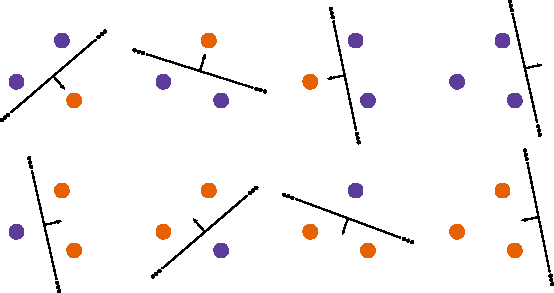
\includegraphics[width=0.85\textwidth]{Figs/PDF/allpossibler3}
        \caption[Possible labellings of 3 points in $\mathbb{R}^2$. ]{\textbf{Possible labellings of 3 points in $\mathbb{R}^2$.} All possible labellings of 3 points in $\mathbb{R}^2$ can be separated by a oriented line (2D hyperplane). This is not possible for all labellings of 4 points in $\mathbb{R}^2$ however, and thus the \gls{vc} dimension of oriented hyperplanes in $\mathbb{R}^2$ is 3. Inspired by figure in \citet{burges1998tutorial}.}\label{fig:vcdim_r2line}
    \end{figure}
    The information theoretic notion of capacity, that is the expressive power of a classification algorithm, gives important insights to the learning ability of a classification algorithm. Analysis is typically based on the Vapnik–Chervonenkis (\gls{vc}) dimension~\citep{vapnik2015uniform} of the class of functions used as discriminators, \eg hyperplanes in the case of neural networks\index{neural network}. Intuitively, for a discriminative classifier, the \gls{vc} dimension measures the largest number of points that can be classified without error. In such a case, the set of points is said to be \emph{shattered} by the classifier. A good overview of \gls{vc} dimension is given by \citet{burges1998tutorial}.
    
    \subsection{Vapnik-Chervonenkis Dimension}
    More formally, a classification model $f(\theta)$, parametrized by $\theta$ is said to \emph{shatter} a set of data points $(x_0, x_1, \ldots, x_h)$ if for for all possible labellings of the points, the classification model can perfectly learn the points. The \gls{vc} dimension is the largest number of (any) points that can be shattered by such a classifier. For a classifier of \gls{vc} dimension $h$, it is sufficient that there exists a \emph{single} set of $h$ points which can be shattered. It is important to note that in general a classifier with a \gls{vc} dimension of $h$ will not necessarily shatter every possible set of $h$ points. 
    %Note that, if the \gls{vc} dimension is h, then there exists at least one set of h points that can be shattered, but it in general it will not be true that every set of h points can be shattered
    
    For example, in \cref{fig:vcdim_r2line}, the function class of oriented hyperplanes, \ie lines in 2D, can separate all possible labellings of 3 points in $\mathbb{R}^2$ --- oriented hyperplanes in $\mathbb{R}^2$ shatter 3 points. However, for 4 points, this is no longer true. It can be proven (see \citet{burges1998tutorial}) that in general for $\mathbb{R}^n$, the set of oriented hyperplanes shatters any set of $n+1$ points.

    The \gls{vc} dimension gives us a measure of the theoretical learning capacity of a classifier, however it can also be somewhat counter-intuitive. While models with large numbers of parameters usually will have a higher \gls{vc} dimension, there are examples of small single parameter models with infinite \gls{vc} dimension for more specific sets of points. For example, if we have a set of evenly spaced points in 2D, a simple sinusoidal curve with the appropriate phase can shatter any labelling of an infinite number of such points. In general, however, such a classifier would be poor at classifying more general sets of points, despite the impressive theoretical \gls{vc} dimension.
    
    \subsection{VC Dimension of Neural Networks}
    In the case of neural networks\index{neural network}, early work showed that the capacity of neural networks\index{neural network} to be quite large~\citep{hornik89a,baum1989size}. \citet{baum1989size} looked at feed-forward networks of \emph{threshold units}, \ie perceptrons\index{perceptron}. %showing the VC dimension of a single-layer network with k units and w weights (including biases) to be bounded by,
    %\begin{equation}
    %    d_{\textrm{VC}} \leq 2 w \log_2(e\,k),
    %\end{equation}
    
    %where $e$ is the mathematical constant, the base of natural logarithms. 
    The authors prove a lower bound on the \gls{vc} dimension for a single hidden layer network of $k$ units and $n$ inputs,
    \begin{equation}
        d_{\textrm{\gls{vc}}} \geq 2 \lfloor k/2 \rfloor n,
    \end{equation}
    where $\lfloor \ \ \rfloor$ is the floor operation, \ie largest integer less than or equal to the operand, and $d$ is the number of inputs. For a single hidden layer network with a large number of $n$ inputs and $k$ units, the authors make the assumption that $kn\approx w$, \ie the number of weights in the first layer alone is approximately that of the whole network $w$,
    \begin{equation}
        d_{\textrm{\gls{vc}}} \geq w.
    \end{equation}

    \citet{baum1989size} use this lower bound on the \gls{vc} dimension of a hidden layer to bound the number of training samples required to achieve an error rate of $\epsilon$, showing that for a network with $w$ weights, and a desired error rate $\epsilon$ the minimum number of training samples required is given by,
    
    \begin{equation}
        N_{\min} \approx w/\epsilon.
    \end{equation}
    
    For an error rate of $\epsilon=0.1$, this gives the rule of thumb that for a network with a total of $w$ weights, approximately $10\times w$, or 10 times the number of training samples as weights in the network, are required to guarantee an error rate of 10\%. 
    
    At first glance this work may seem to have solved a major problem in the design and training of neural networks\index{neural network}, however the work of \citet{baum1989size} is to show a worst-case lower bound on the number of training samples required --- in practice this can be far from what is empirically required. \citet{baum1989size} themselves point out that this is likely be far more than necessary in networks where the learning algorithm seeks to minimize the number of non-zero weights (such as networks using weight decay, pruning, etc). Indeed, in practice neural networks\index{neural network} were found to generalize much better than this worst case bound would indicate, to the point where modern deep neural networks\index{neural network} are trained with far fewer samples than weights, in the case of AlexNet~\citep{Krizhevsky2012} approximately $250\times$ \emph{fewer} training samples than weights allows good generalization on the \gls{ilsvrc}~\citep{ILSVRC2015} dataset.
    
    \citet{bartlett1997} later showed that rather than capacity being based on solely the number of weights, a bound more in-line with empirical results could be found by using the number of \emph{large weights}. To show this they moved to a scale sensitive form of the \gls{vc} dimension, the \emph{fat-shattering} dimension. The author shows that the error rate for an $\ell$-layer sigmoidal (rather than threshold unit) neural network\index{neural network} with $n$ inputs and $m$ training samples,
    
    \begin{equation}
        \epsilon \approx (cA)^{\ell(\ell+1)/2} \sqrt{(\log n)/m},
    \end{equation}
    
    and $c$ is a constant factor, and the $\ell_1$ norm of each unit's weight vector $w$ is bounded by $A$, 
    \begin{equation}
    \|\mathbf{w}\|_1 = \sum_i | w_i | \leq A.
    \end{equation}
    Surprisingly there is no term for the number of units for any layer in this equation, but rather it is the bounds on the weights themselves that determine ability of the network to generalize. In general, for a network where the inputs $\mathbf{x}$ are also bounded,
    \begin{equation}
        \|\mathbf{x}\|_\infty = \max(|x_0|, |x_1|, \ldots, |x_n|) \leq B,
    \end{equation}
    \citet{bartlett1997} show that for a given error $\epsilon$, the number of training samples $m$ required grows roughly as,
    \begin{align}
        m \approx \frac{B^2\,A^{\ell^2}}{\epsilon^2}.
    \end{align}
    
     For a single hidden layer network, \ie $\ell=2$, and an error rate of $\epsilon=0.05$, 
    
    \begin{align}
        m \approx 400\,B^2\,A^6.
    \end{align}
    
    This result, while surprising given the analysis based on the \gls{vc} dimension of neural networks\index{neural network}, supports empirical results in using contemporary training methods such as weight decay~\citep{hinton1987learning}, early stopping~\citep{Bishop1995}, and even more recently batch normalization~\citep{Ioffe2015}, all of which can keep weight magnitudes low.
%    For a single hidden layer network, \ie $\ell=2$, and an error rate of $\epsilon=0.05$, 
    
%    \begin{align}
%        m &\approx  \frac{\log n \, (cA)^{\ell(\ell+1)}}{\epsilon^2}\\
%        &\approx  \frac{\log n \, (cA)^{6}}{0.0025},\\
%    \end{align}
%    we can see that the number of training samples required to guarantee this error rate are proportional to the logarithm of the number of inputs and the , 
	
    \subsection{Model Size}
    \mynote{TODO: Include references to \citet{baum1989size, rethinking2016}}
    
	\begin{figure}[tb]
		\centering
		\begin{subfigure}[t]{0.49\textwidth}
			\resizebox{\linewidth}{!}{%% Creator: Matplotlib, PGF backend
%%
%% To include the figure in your LaTeX document, write
%%   \input{<filename>.pgf}
%%
%% Make sure the required packages are loaded in your preamble
%%   \usepackage{pgf}
%%
%% Figures using additional raster images can only be included by \input if
%% they are in the same directory as the main LaTeX file. For loading figures
%% from other directories you can use the `import` package
%%   \usepackage{import}
%% and then include the figures with
%%   \import{<path to file>}{<filename>.pgf}
%%
%% Matplotlib used the following preamble
%%   \usepackage[utf8x]{inputenc}
%%   \usepackage[T1]{fontenc}
%%
\begingroup%
\makeatletter%
\begin{pgfpicture}%
\pgfpathrectangle{\pgfpointorigin}{\pgfqpoint{4.296389in}{2.655314in}}%
\pgfusepath{use as bounding box, clip}%
\begin{pgfscope}%
\pgfsetbuttcap%
\pgfsetmiterjoin%
\definecolor{currentfill}{rgb}{1.000000,1.000000,1.000000}%
\pgfsetfillcolor{currentfill}%
\pgfsetlinewidth{0.000000pt}%
\definecolor{currentstroke}{rgb}{1.000000,1.000000,1.000000}%
\pgfsetstrokecolor{currentstroke}%
\pgfsetdash{}{0pt}%
\pgfpathmoveto{\pgfqpoint{0.000000in}{0.000000in}}%
\pgfpathlineto{\pgfqpoint{4.296389in}{0.000000in}}%
\pgfpathlineto{\pgfqpoint{4.296389in}{2.655314in}}%
\pgfpathlineto{\pgfqpoint{0.000000in}{2.655314in}}%
\pgfpathclose%
\pgfusepath{fill}%
\end{pgfscope}%
\begin{pgfscope}%
\pgfsetbuttcap%
\pgfsetmiterjoin%
\definecolor{currentfill}{rgb}{1.000000,1.000000,1.000000}%
\pgfsetfillcolor{currentfill}%
\pgfsetlinewidth{0.000000pt}%
\definecolor{currentstroke}{rgb}{0.000000,0.000000,0.000000}%
\pgfsetstrokecolor{currentstroke}%
\pgfsetstrokeopacity{0.000000}%
\pgfsetdash{}{0pt}%
\pgfpathmoveto{\pgfqpoint{0.548317in}{0.386884in}}%
\pgfpathlineto{\pgfqpoint{4.124652in}{0.386884in}}%
\pgfpathlineto{\pgfqpoint{4.124652in}{2.488647in}}%
\pgfpathlineto{\pgfqpoint{0.548317in}{2.488647in}}%
\pgfpathclose%
\pgfusepath{fill}%
\end{pgfscope}%
\begin{pgfscope}%
\pgfsetbuttcap%
\pgfsetroundjoin%
\definecolor{currentfill}{rgb}{0.150000,0.150000,0.150000}%
\pgfsetfillcolor{currentfill}%
\pgfsetlinewidth{1.003750pt}%
\definecolor{currentstroke}{rgb}{0.150000,0.150000,0.150000}%
\pgfsetstrokecolor{currentstroke}%
\pgfsetdash{}{0pt}%
\pgfsys@defobject{currentmarker}{\pgfqpoint{0.000000in}{-0.083333in}}{\pgfqpoint{0.000000in}{0.000000in}}{%
\pgfpathmoveto{\pgfqpoint{0.000000in}{0.000000in}}%
\pgfpathlineto{\pgfqpoint{0.000000in}{-0.083333in}}%
\pgfusepath{stroke,fill}%
}%
\begin{pgfscope}%
\pgfsys@transformshift{0.548317in}{0.386884in}%
\pgfsys@useobject{currentmarker}{}%
\end{pgfscope}%
\end{pgfscope}%
\begin{pgfscope}%
\definecolor{textcolor}{rgb}{0.150000,0.150000,0.150000}%
\pgfsetstrokecolor{textcolor}%
\pgfsetfillcolor{textcolor}%
\pgftext[x=0.548317in,y=0.206329in,,top]{\color{textcolor}\sffamily\fontsize{10.000000}{12.000000}\selectfont \(\displaystyle 0.0\)}%
\end{pgfscope}%
\begin{pgfscope}%
\pgfsetbuttcap%
\pgfsetroundjoin%
\definecolor{currentfill}{rgb}{0.150000,0.150000,0.150000}%
\pgfsetfillcolor{currentfill}%
\pgfsetlinewidth{1.003750pt}%
\definecolor{currentstroke}{rgb}{0.150000,0.150000,0.150000}%
\pgfsetstrokecolor{currentstroke}%
\pgfsetdash{}{0pt}%
\pgfsys@defobject{currentmarker}{\pgfqpoint{0.000000in}{-0.083333in}}{\pgfqpoint{0.000000in}{0.000000in}}{%
\pgfpathmoveto{\pgfqpoint{0.000000in}{0.000000in}}%
\pgfpathlineto{\pgfqpoint{0.000000in}{-0.083333in}}%
\pgfusepath{stroke,fill}%
}%
\begin{pgfscope}%
\pgfsys@transformshift{1.263584in}{0.386884in}%
\pgfsys@useobject{currentmarker}{}%
\end{pgfscope}%
\end{pgfscope}%
\begin{pgfscope}%
\definecolor{textcolor}{rgb}{0.150000,0.150000,0.150000}%
\pgfsetstrokecolor{textcolor}%
\pgfsetfillcolor{textcolor}%
\pgftext[x=1.263584in,y=0.206329in,,top]{\color{textcolor}\sffamily\fontsize{10.000000}{12.000000}\selectfont \(\displaystyle 0.2\)}%
\end{pgfscope}%
\begin{pgfscope}%
\pgfsetbuttcap%
\pgfsetroundjoin%
\definecolor{currentfill}{rgb}{0.150000,0.150000,0.150000}%
\pgfsetfillcolor{currentfill}%
\pgfsetlinewidth{1.003750pt}%
\definecolor{currentstroke}{rgb}{0.150000,0.150000,0.150000}%
\pgfsetstrokecolor{currentstroke}%
\pgfsetdash{}{0pt}%
\pgfsys@defobject{currentmarker}{\pgfqpoint{0.000000in}{-0.083333in}}{\pgfqpoint{0.000000in}{0.000000in}}{%
\pgfpathmoveto{\pgfqpoint{0.000000in}{0.000000in}}%
\pgfpathlineto{\pgfqpoint{0.000000in}{-0.083333in}}%
\pgfusepath{stroke,fill}%
}%
\begin{pgfscope}%
\pgfsys@transformshift{1.978851in}{0.386884in}%
\pgfsys@useobject{currentmarker}{}%
\end{pgfscope}%
\end{pgfscope}%
\begin{pgfscope}%
\definecolor{textcolor}{rgb}{0.150000,0.150000,0.150000}%
\pgfsetstrokecolor{textcolor}%
\pgfsetfillcolor{textcolor}%
\pgftext[x=1.978851in,y=0.206329in,,top]{\color{textcolor}\sffamily\fontsize{10.000000}{12.000000}\selectfont \(\displaystyle 0.4\)}%
\end{pgfscope}%
\begin{pgfscope}%
\pgfsetbuttcap%
\pgfsetroundjoin%
\definecolor{currentfill}{rgb}{0.150000,0.150000,0.150000}%
\pgfsetfillcolor{currentfill}%
\pgfsetlinewidth{1.003750pt}%
\definecolor{currentstroke}{rgb}{0.150000,0.150000,0.150000}%
\pgfsetstrokecolor{currentstroke}%
\pgfsetdash{}{0pt}%
\pgfsys@defobject{currentmarker}{\pgfqpoint{0.000000in}{-0.083333in}}{\pgfqpoint{0.000000in}{0.000000in}}{%
\pgfpathmoveto{\pgfqpoint{0.000000in}{0.000000in}}%
\pgfpathlineto{\pgfqpoint{0.000000in}{-0.083333in}}%
\pgfusepath{stroke,fill}%
}%
\begin{pgfscope}%
\pgfsys@transformshift{2.694118in}{0.386884in}%
\pgfsys@useobject{currentmarker}{}%
\end{pgfscope}%
\end{pgfscope}%
\begin{pgfscope}%
\definecolor{textcolor}{rgb}{0.150000,0.150000,0.150000}%
\pgfsetstrokecolor{textcolor}%
\pgfsetfillcolor{textcolor}%
\pgftext[x=2.694118in,y=0.206329in,,top]{\color{textcolor}\sffamily\fontsize{10.000000}{12.000000}\selectfont \(\displaystyle 0.6\)}%
\end{pgfscope}%
\begin{pgfscope}%
\pgfsetbuttcap%
\pgfsetroundjoin%
\definecolor{currentfill}{rgb}{0.150000,0.150000,0.150000}%
\pgfsetfillcolor{currentfill}%
\pgfsetlinewidth{1.003750pt}%
\definecolor{currentstroke}{rgb}{0.150000,0.150000,0.150000}%
\pgfsetstrokecolor{currentstroke}%
\pgfsetdash{}{0pt}%
\pgfsys@defobject{currentmarker}{\pgfqpoint{0.000000in}{-0.083333in}}{\pgfqpoint{0.000000in}{0.000000in}}{%
\pgfpathmoveto{\pgfqpoint{0.000000in}{0.000000in}}%
\pgfpathlineto{\pgfqpoint{0.000000in}{-0.083333in}}%
\pgfusepath{stroke,fill}%
}%
\begin{pgfscope}%
\pgfsys@transformshift{3.409385in}{0.386884in}%
\pgfsys@useobject{currentmarker}{}%
\end{pgfscope}%
\end{pgfscope}%
\begin{pgfscope}%
\definecolor{textcolor}{rgb}{0.150000,0.150000,0.150000}%
\pgfsetstrokecolor{textcolor}%
\pgfsetfillcolor{textcolor}%
\pgftext[x=3.409385in,y=0.206329in,,top]{\color{textcolor}\sffamily\fontsize{10.000000}{12.000000}\selectfont \(\displaystyle 0.8\)}%
\end{pgfscope}%
\begin{pgfscope}%
\pgfsetbuttcap%
\pgfsetroundjoin%
\definecolor{currentfill}{rgb}{0.150000,0.150000,0.150000}%
\pgfsetfillcolor{currentfill}%
\pgfsetlinewidth{1.003750pt}%
\definecolor{currentstroke}{rgb}{0.150000,0.150000,0.150000}%
\pgfsetstrokecolor{currentstroke}%
\pgfsetdash{}{0pt}%
\pgfsys@defobject{currentmarker}{\pgfqpoint{0.000000in}{-0.083333in}}{\pgfqpoint{0.000000in}{0.000000in}}{%
\pgfpathmoveto{\pgfqpoint{0.000000in}{0.000000in}}%
\pgfpathlineto{\pgfqpoint{0.000000in}{-0.083333in}}%
\pgfusepath{stroke,fill}%
}%
\begin{pgfscope}%
\pgfsys@transformshift{4.124652in}{0.386884in}%
\pgfsys@useobject{currentmarker}{}%
\end{pgfscope}%
\end{pgfscope}%
\begin{pgfscope}%
\definecolor{textcolor}{rgb}{0.150000,0.150000,0.150000}%
\pgfsetstrokecolor{textcolor}%
\pgfsetfillcolor{textcolor}%
\pgftext[x=4.124652in,y=0.206329in,,top]{\color{textcolor}\sffamily\fontsize{10.000000}{12.000000}\selectfont \(\displaystyle 1.0\)}%
\end{pgfscope}%
\begin{pgfscope}%
\pgfsetbuttcap%
\pgfsetroundjoin%
\definecolor{currentfill}{rgb}{0.150000,0.150000,0.150000}%
\pgfsetfillcolor{currentfill}%
\pgfsetlinewidth{1.003750pt}%
\definecolor{currentstroke}{rgb}{0.150000,0.150000,0.150000}%
\pgfsetstrokecolor{currentstroke}%
\pgfsetdash{}{0pt}%
\pgfsys@defobject{currentmarker}{\pgfqpoint{-0.083333in}{0.000000in}}{\pgfqpoint{0.000000in}{0.000000in}}{%
\pgfpathmoveto{\pgfqpoint{0.000000in}{0.000000in}}%
\pgfpathlineto{\pgfqpoint{-0.083333in}{0.000000in}}%
\pgfusepath{stroke,fill}%
}%
\begin{pgfscope}%
\pgfsys@transformshift{0.548317in}{0.386884in}%
\pgfsys@useobject{currentmarker}{}%
\end{pgfscope}%
\end{pgfscope}%
\begin{pgfscope}%
\definecolor{textcolor}{rgb}{0.150000,0.150000,0.150000}%
\pgfsetstrokecolor{textcolor}%
\pgfsetfillcolor{textcolor}%
\pgftext[x=0.082267in,y=0.336742in,left,base]{\color{textcolor}\sffamily\fontsize{10.000000}{12.000000}\selectfont \(\displaystyle -1.0\)}%
\end{pgfscope}%
\begin{pgfscope}%
\pgfsetbuttcap%
\pgfsetroundjoin%
\definecolor{currentfill}{rgb}{0.150000,0.150000,0.150000}%
\pgfsetfillcolor{currentfill}%
\pgfsetlinewidth{1.003750pt}%
\definecolor{currentstroke}{rgb}{0.150000,0.150000,0.150000}%
\pgfsetstrokecolor{currentstroke}%
\pgfsetdash{}{0pt}%
\pgfsys@defobject{currentmarker}{\pgfqpoint{-0.083333in}{0.000000in}}{\pgfqpoint{0.000000in}{0.000000in}}{%
\pgfpathmoveto{\pgfqpoint{0.000000in}{0.000000in}}%
\pgfpathlineto{\pgfqpoint{-0.083333in}{0.000000in}}%
\pgfusepath{stroke,fill}%
}%
\begin{pgfscope}%
\pgfsys@transformshift{0.548317in}{0.912325in}%
\pgfsys@useobject{currentmarker}{}%
\end{pgfscope}%
\end{pgfscope}%
\begin{pgfscope}%
\definecolor{textcolor}{rgb}{0.150000,0.150000,0.150000}%
\pgfsetstrokecolor{textcolor}%
\pgfsetfillcolor{textcolor}%
\pgftext[x=0.082267in,y=0.862183in,left,base]{\color{textcolor}\sffamily\fontsize{10.000000}{12.000000}\selectfont \(\displaystyle -0.5\)}%
\end{pgfscope}%
\begin{pgfscope}%
\pgfsetbuttcap%
\pgfsetroundjoin%
\definecolor{currentfill}{rgb}{0.150000,0.150000,0.150000}%
\pgfsetfillcolor{currentfill}%
\pgfsetlinewidth{1.003750pt}%
\definecolor{currentstroke}{rgb}{0.150000,0.150000,0.150000}%
\pgfsetstrokecolor{currentstroke}%
\pgfsetdash{}{0pt}%
\pgfsys@defobject{currentmarker}{\pgfqpoint{-0.083333in}{0.000000in}}{\pgfqpoint{0.000000in}{0.000000in}}{%
\pgfpathmoveto{\pgfqpoint{0.000000in}{0.000000in}}%
\pgfpathlineto{\pgfqpoint{-0.083333in}{0.000000in}}%
\pgfusepath{stroke,fill}%
}%
\begin{pgfscope}%
\pgfsys@transformshift{0.548317in}{1.437766in}%
\pgfsys@useobject{currentmarker}{}%
\end{pgfscope}%
\end{pgfscope}%
\begin{pgfscope}%
\definecolor{textcolor}{rgb}{0.150000,0.150000,0.150000}%
\pgfsetstrokecolor{textcolor}%
\pgfsetfillcolor{textcolor}%
\pgftext[x=0.190292in,y=1.387624in,left,base]{\color{textcolor}\sffamily\fontsize{10.000000}{12.000000}\selectfont \(\displaystyle 0.0\)}%
\end{pgfscope}%
\begin{pgfscope}%
\pgfsetbuttcap%
\pgfsetroundjoin%
\definecolor{currentfill}{rgb}{0.150000,0.150000,0.150000}%
\pgfsetfillcolor{currentfill}%
\pgfsetlinewidth{1.003750pt}%
\definecolor{currentstroke}{rgb}{0.150000,0.150000,0.150000}%
\pgfsetstrokecolor{currentstroke}%
\pgfsetdash{}{0pt}%
\pgfsys@defobject{currentmarker}{\pgfqpoint{-0.083333in}{0.000000in}}{\pgfqpoint{0.000000in}{0.000000in}}{%
\pgfpathmoveto{\pgfqpoint{0.000000in}{0.000000in}}%
\pgfpathlineto{\pgfqpoint{-0.083333in}{0.000000in}}%
\pgfusepath{stroke,fill}%
}%
\begin{pgfscope}%
\pgfsys@transformshift{0.548317in}{1.963207in}%
\pgfsys@useobject{currentmarker}{}%
\end{pgfscope}%
\end{pgfscope}%
\begin{pgfscope}%
\definecolor{textcolor}{rgb}{0.150000,0.150000,0.150000}%
\pgfsetstrokecolor{textcolor}%
\pgfsetfillcolor{textcolor}%
\pgftext[x=0.190292in,y=1.913065in,left,base]{\color{textcolor}\sffamily\fontsize{10.000000}{12.000000}\selectfont \(\displaystyle 0.5\)}%
\end{pgfscope}%
\begin{pgfscope}%
\pgfsetbuttcap%
\pgfsetroundjoin%
\definecolor{currentfill}{rgb}{0.150000,0.150000,0.150000}%
\pgfsetfillcolor{currentfill}%
\pgfsetlinewidth{1.003750pt}%
\definecolor{currentstroke}{rgb}{0.150000,0.150000,0.150000}%
\pgfsetstrokecolor{currentstroke}%
\pgfsetdash{}{0pt}%
\pgfsys@defobject{currentmarker}{\pgfqpoint{-0.083333in}{0.000000in}}{\pgfqpoint{0.000000in}{0.000000in}}{%
\pgfpathmoveto{\pgfqpoint{0.000000in}{0.000000in}}%
\pgfpathlineto{\pgfqpoint{-0.083333in}{0.000000in}}%
\pgfusepath{stroke,fill}%
}%
\begin{pgfscope}%
\pgfsys@transformshift{0.548317in}{2.488647in}%
\pgfsys@useobject{currentmarker}{}%
\end{pgfscope}%
\end{pgfscope}%
\begin{pgfscope}%
\definecolor{textcolor}{rgb}{0.150000,0.150000,0.150000}%
\pgfsetstrokecolor{textcolor}%
\pgfsetfillcolor{textcolor}%
\pgftext[x=0.190292in,y=2.438505in,left,base]{\color{textcolor}\sffamily\fontsize{10.000000}{12.000000}\selectfont \(\displaystyle 1.0\)}%
\end{pgfscope}%
\begin{pgfscope}%
\pgfpathrectangle{\pgfqpoint{0.548317in}{0.386884in}}{\pgfqpoint{3.576335in}{2.101763in}} %
\pgfusepath{clip}%
\pgfsetbuttcap%
\pgfsetroundjoin%
\definecolor{currentfill}{rgb}{0.400000,0.760784,0.647059}%
\pgfsetfillcolor{currentfill}%
\pgfsetlinewidth{0.000000pt}%
\definecolor{currentstroke}{rgb}{0.400000,0.760784,0.647059}%
\pgfsetstrokecolor{currentstroke}%
\pgfsetdash{}{0pt}%
\pgfsys@defobject{currentmarker}{\pgfqpoint{-0.048611in}{-0.048611in}}{\pgfqpoint{0.048611in}{0.048611in}}{%
\pgfpathmoveto{\pgfqpoint{0.000000in}{-0.048611in}}%
\pgfpathcurveto{\pgfqpoint{0.012892in}{-0.048611in}}{\pgfqpoint{0.025257in}{-0.043489in}}{\pgfqpoint{0.034373in}{-0.034373in}}%
\pgfpathcurveto{\pgfqpoint{0.043489in}{-0.025257in}}{\pgfqpoint{0.048611in}{-0.012892in}}{\pgfqpoint{0.048611in}{0.000000in}}%
\pgfpathcurveto{\pgfqpoint{0.048611in}{0.012892in}}{\pgfqpoint{0.043489in}{0.025257in}}{\pgfqpoint{0.034373in}{0.034373in}}%
\pgfpathcurveto{\pgfqpoint{0.025257in}{0.043489in}}{\pgfqpoint{0.012892in}{0.048611in}}{\pgfqpoint{0.000000in}{0.048611in}}%
\pgfpathcurveto{\pgfqpoint{-0.012892in}{0.048611in}}{\pgfqpoint{-0.025257in}{0.043489in}}{\pgfqpoint{-0.034373in}{0.034373in}}%
\pgfpathcurveto{\pgfqpoint{-0.043489in}{0.025257in}}{\pgfqpoint{-0.048611in}{0.012892in}}{\pgfqpoint{-0.048611in}{0.000000in}}%
\pgfpathcurveto{\pgfqpoint{-0.048611in}{-0.012892in}}{\pgfqpoint{-0.043489in}{-0.025257in}}{\pgfqpoint{-0.034373in}{-0.034373in}}%
\pgfpathcurveto{\pgfqpoint{-0.025257in}{-0.043489in}}{\pgfqpoint{-0.012892in}{-0.048611in}}{\pgfqpoint{0.000000in}{-0.048611in}}%
\pgfpathclose%
\pgfusepath{fill}%
}%
\begin{pgfscope}%
\pgfsys@transformshift{2.260811in}{0.754316in}%
\pgfsys@useobject{currentmarker}{}%
\end{pgfscope}%
\begin{pgfscope}%
\pgfsys@transformshift{2.611975in}{0.899184in}%
\pgfsys@useobject{currentmarker}{}%
\end{pgfscope}%
\begin{pgfscope}%
\pgfsys@transformshift{3.012052in}{1.144101in}%
\pgfsys@useobject{currentmarker}{}%
\end{pgfscope}%
\end{pgfscope}%
\begin{pgfscope}%
\pgfpathrectangle{\pgfqpoint{0.548317in}{0.386884in}}{\pgfqpoint{3.576335in}{2.101763in}} %
\pgfusepath{clip}%
\pgfsetbuttcap%
\pgfsetroundjoin%
\pgfsetlinewidth{1.756562pt}%
\definecolor{currentstroke}{rgb}{0.988235,0.552941,0.384314}%
\pgfsetstrokecolor{currentstroke}%
\pgfsetdash{{5.600000pt}{2.400000pt}}{0.000000pt}%
\pgfpathmoveto{\pgfqpoint{0.534428in}{0.382588in}}%
\pgfpathlineto{\pgfqpoint{0.584442in}{0.397288in}}%
\pgfpathlineto{\pgfqpoint{0.656691in}{0.416887in}}%
\pgfpathlineto{\pgfqpoint{0.728940in}{0.435004in}}%
\pgfpathlineto{\pgfqpoint{0.801189in}{0.451796in}}%
\pgfpathlineto{\pgfqpoint{0.873438in}{0.467418in}}%
\pgfpathlineto{\pgfqpoint{0.945688in}{0.482026in}}%
\pgfpathlineto{\pgfqpoint{1.017937in}{0.495776in}}%
\pgfpathlineto{\pgfqpoint{1.090186in}{0.508825in}}%
\pgfpathlineto{\pgfqpoint{1.162435in}{0.521328in}}%
\pgfpathlineto{\pgfqpoint{1.234684in}{0.533440in}}%
\pgfpathlineto{\pgfqpoint{1.306933in}{0.545319in}}%
\pgfpathlineto{\pgfqpoint{1.379183in}{0.557120in}}%
\pgfpathlineto{\pgfqpoint{1.451432in}{0.568999in}}%
\pgfpathlineto{\pgfqpoint{1.523681in}{0.581112in}}%
\pgfpathlineto{\pgfqpoint{1.595930in}{0.593615in}}%
\pgfpathlineto{\pgfqpoint{1.668179in}{0.606663in}}%
\pgfpathlineto{\pgfqpoint{1.740429in}{0.620414in}}%
\pgfpathlineto{\pgfqpoint{1.812678in}{0.635022in}}%
\pgfpathlineto{\pgfqpoint{1.884927in}{0.650644in}}%
\pgfpathlineto{\pgfqpoint{1.957176in}{0.667435in}}%
\pgfpathlineto{\pgfqpoint{2.029425in}{0.685553in}}%
\pgfpathlineto{\pgfqpoint{2.101675in}{0.705151in}}%
\pgfpathlineto{\pgfqpoint{2.173924in}{0.726388in}}%
\pgfpathlineto{\pgfqpoint{2.246173in}{0.749418in}}%
\pgfpathlineto{\pgfqpoint{2.318422in}{0.774397in}}%
\pgfpathlineto{\pgfqpoint{2.390671in}{0.801482in}}%
\pgfpathlineto{\pgfqpoint{2.462921in}{0.830828in}}%
\pgfpathlineto{\pgfqpoint{2.535170in}{0.862592in}}%
\pgfpathlineto{\pgfqpoint{2.607419in}{0.896929in}}%
\pgfpathlineto{\pgfqpoint{2.679668in}{0.933995in}}%
\pgfpathlineto{\pgfqpoint{2.751917in}{0.973947in}}%
\pgfpathlineto{\pgfqpoint{2.824166in}{1.016940in}}%
\pgfpathlineto{\pgfqpoint{2.896416in}{1.063129in}}%
\pgfpathlineto{\pgfqpoint{2.968665in}{1.112672in}}%
\pgfpathlineto{\pgfqpoint{3.040914in}{1.165725in}}%
\pgfpathlineto{\pgfqpoint{3.113163in}{1.222442in}}%
\pgfpathlineto{\pgfqpoint{3.185412in}{1.282980in}}%
\pgfpathlineto{\pgfqpoint{3.257662in}{1.347495in}}%
\pgfpathlineto{\pgfqpoint{3.329911in}{1.416143in}}%
\pgfpathlineto{\pgfqpoint{3.402160in}{1.489080in}}%
\pgfpathlineto{\pgfqpoint{3.474409in}{1.566461in}}%
\pgfpathlineto{\pgfqpoint{3.546658in}{1.648444in}}%
\pgfpathlineto{\pgfqpoint{3.618908in}{1.735183in}}%
\pgfpathlineto{\pgfqpoint{3.691157in}{1.826835in}}%
\pgfpathlineto{\pgfqpoint{3.763406in}{1.923556in}}%
\pgfpathlineto{\pgfqpoint{3.835655in}{2.025501in}}%
\pgfpathlineto{\pgfqpoint{3.907904in}{2.132827in}}%
\pgfpathlineto{\pgfqpoint{3.980154in}{2.245689in}}%
\pgfpathlineto{\pgfqpoint{4.052403in}{2.364244in}}%
\pgfpathlineto{\pgfqpoint{4.124652in}{2.488647in}}%
\pgfusepath{stroke}%
\end{pgfscope}%
\begin{pgfscope}%
\pgfpathrectangle{\pgfqpoint{0.548317in}{0.386884in}}{\pgfqpoint{3.576335in}{2.101763in}} %
\pgfusepath{clip}%
\pgfsetroundcap%
\pgfsetroundjoin%
\pgfsetlinewidth{1.756562pt}%
\definecolor{currentstroke}{rgb}{0.552941,0.627451,0.796078}%
\pgfsetstrokecolor{currentstroke}%
\pgfsetdash{}{0pt}%
\pgfpathmoveto{\pgfqpoint{0.534428in}{0.664235in}}%
\pgfpathlineto{\pgfqpoint{0.584442in}{0.658600in}}%
\pgfpathlineto{\pgfqpoint{0.656691in}{0.650850in}}%
\pgfpathlineto{\pgfqpoint{0.728940in}{0.643574in}}%
\pgfpathlineto{\pgfqpoint{0.801189in}{0.636856in}}%
\pgfpathlineto{\pgfqpoint{0.873438in}{0.630780in}}%
\pgfpathlineto{\pgfqpoint{0.945688in}{0.625432in}}%
\pgfpathlineto{\pgfqpoint{1.017937in}{0.620894in}}%
\pgfpathlineto{\pgfqpoint{1.090186in}{0.617252in}}%
\pgfpathlineto{\pgfqpoint{1.162435in}{0.614590in}}%
\pgfpathlineto{\pgfqpoint{1.234684in}{0.612992in}}%
\pgfpathlineto{\pgfqpoint{1.306933in}{0.612542in}}%
\pgfpathlineto{\pgfqpoint{1.379183in}{0.613325in}}%
\pgfpathlineto{\pgfqpoint{1.451432in}{0.615424in}}%
\pgfpathlineto{\pgfqpoint{1.523681in}{0.618925in}}%
\pgfpathlineto{\pgfqpoint{1.595930in}{0.623912in}}%
\pgfpathlineto{\pgfqpoint{1.668179in}{0.630468in}}%
\pgfpathlineto{\pgfqpoint{1.740429in}{0.638678in}}%
\pgfpathlineto{\pgfqpoint{1.812678in}{0.648627in}}%
\pgfpathlineto{\pgfqpoint{1.884927in}{0.660399in}}%
\pgfpathlineto{\pgfqpoint{1.957176in}{0.674077in}}%
\pgfpathlineto{\pgfqpoint{2.029425in}{0.689747in}}%
\pgfpathlineto{\pgfqpoint{2.101675in}{0.707493in}}%
\pgfpathlineto{\pgfqpoint{2.173924in}{0.727398in}}%
\pgfpathlineto{\pgfqpoint{2.246173in}{0.749548in}}%
\pgfpathlineto{\pgfqpoint{2.318422in}{0.774026in}}%
\pgfpathlineto{\pgfqpoint{2.390671in}{0.800917in}}%
\pgfpathlineto{\pgfqpoint{2.462921in}{0.830305in}}%
\pgfpathlineto{\pgfqpoint{2.535170in}{0.862274in}}%
\pgfpathlineto{\pgfqpoint{2.607419in}{0.896909in}}%
\pgfpathlineto{\pgfqpoint{2.679668in}{0.934294in}}%
\pgfpathlineto{\pgfqpoint{2.751917in}{0.974513in}}%
\pgfpathlineto{\pgfqpoint{2.824166in}{1.017651in}}%
\pgfpathlineto{\pgfqpoint{2.896416in}{1.063792in}}%
\pgfpathlineto{\pgfqpoint{2.968665in}{1.113019in}}%
\pgfpathlineto{\pgfqpoint{3.040914in}{1.165419in}}%
\pgfpathlineto{\pgfqpoint{3.113163in}{1.221074in}}%
\pgfpathlineto{\pgfqpoint{3.185412in}{1.280069in}}%
\pgfpathlineto{\pgfqpoint{3.257662in}{1.342488in}}%
\pgfpathlineto{\pgfqpoint{3.329911in}{1.408416in}}%
\pgfpathlineto{\pgfqpoint{3.402160in}{1.477937in}}%
\pgfpathlineto{\pgfqpoint{3.474409in}{1.551136in}}%
\pgfpathlineto{\pgfqpoint{3.546658in}{1.628095in}}%
\pgfpathlineto{\pgfqpoint{3.618908in}{1.708901in}}%
\pgfpathlineto{\pgfqpoint{3.691157in}{1.793637in}}%
\pgfpathlineto{\pgfqpoint{3.763406in}{1.882387in}}%
\pgfpathlineto{\pgfqpoint{3.835655in}{1.975236in}}%
\pgfpathlineto{\pgfqpoint{3.907904in}{2.072268in}}%
\pgfpathlineto{\pgfqpoint{3.980154in}{2.173567in}}%
\pgfpathlineto{\pgfqpoint{4.052403in}{2.279218in}}%
\pgfpathlineto{\pgfqpoint{4.124652in}{2.389305in}}%
\pgfusepath{stroke}%
\end{pgfscope}%
\begin{pgfscope}%
\pgfsetrectcap%
\pgfsetmiterjoin%
\pgfsetlinewidth{1.254687pt}%
\definecolor{currentstroke}{rgb}{0.150000,0.150000,0.150000}%
\pgfsetstrokecolor{currentstroke}%
\pgfsetdash{}{0pt}%
\pgfpathmoveto{\pgfqpoint{0.548317in}{0.386884in}}%
\pgfpathlineto{\pgfqpoint{0.548317in}{2.488647in}}%
\pgfusepath{stroke}%
\end{pgfscope}%
\begin{pgfscope}%
\pgfsetrectcap%
\pgfsetmiterjoin%
\pgfsetlinewidth{1.254687pt}%
\definecolor{currentstroke}{rgb}{0.150000,0.150000,0.150000}%
\pgfsetstrokecolor{currentstroke}%
\pgfsetdash{}{0pt}%
\pgfpathmoveto{\pgfqpoint{0.548317in}{0.386884in}}%
\pgfpathlineto{\pgfqpoint{4.124652in}{0.386884in}}%
\pgfusepath{stroke}%
\end{pgfscope}%
\begin{pgfscope}%
\pgfsetbuttcap%
\pgfsetroundjoin%
\definecolor{currentfill}{rgb}{0.400000,0.760784,0.647059}%
\pgfsetfillcolor{currentfill}%
\pgfsetlinewidth{0.000000pt}%
\definecolor{currentstroke}{rgb}{0.400000,0.760784,0.647059}%
\pgfsetstrokecolor{currentstroke}%
\pgfsetdash{}{0pt}%
\pgfsys@defobject{currentmarker}{\pgfqpoint{-0.048611in}{-0.048611in}}{\pgfqpoint{0.048611in}{0.048611in}}{%
\pgfpathmoveto{\pgfqpoint{0.000000in}{-0.048611in}}%
\pgfpathcurveto{\pgfqpoint{0.012892in}{-0.048611in}}{\pgfqpoint{0.025257in}{-0.043489in}}{\pgfqpoint{0.034373in}{-0.034373in}}%
\pgfpathcurveto{\pgfqpoint{0.043489in}{-0.025257in}}{\pgfqpoint{0.048611in}{-0.012892in}}{\pgfqpoint{0.048611in}{0.000000in}}%
\pgfpathcurveto{\pgfqpoint{0.048611in}{0.012892in}}{\pgfqpoint{0.043489in}{0.025257in}}{\pgfqpoint{0.034373in}{0.034373in}}%
\pgfpathcurveto{\pgfqpoint{0.025257in}{0.043489in}}{\pgfqpoint{0.012892in}{0.048611in}}{\pgfqpoint{0.000000in}{0.048611in}}%
\pgfpathcurveto{\pgfqpoint{-0.012892in}{0.048611in}}{\pgfqpoint{-0.025257in}{0.043489in}}{\pgfqpoint{-0.034373in}{0.034373in}}%
\pgfpathcurveto{\pgfqpoint{-0.043489in}{0.025257in}}{\pgfqpoint{-0.048611in}{0.012892in}}{\pgfqpoint{-0.048611in}{0.000000in}}%
\pgfpathcurveto{\pgfqpoint{-0.048611in}{-0.012892in}}{\pgfqpoint{-0.043489in}{-0.025257in}}{\pgfqpoint{-0.034373in}{-0.034373in}}%
\pgfpathcurveto{\pgfqpoint{-0.025257in}{-0.043489in}}{\pgfqpoint{-0.012892in}{-0.048611in}}{\pgfqpoint{0.000000in}{-0.048611in}}%
\pgfpathclose%
\pgfusepath{fill}%
}%
\begin{pgfscope}%
\pgfsys@transformshift{0.812206in}{2.311974in}%
\pgfsys@useobject{currentmarker}{}%
\end{pgfscope}%
\end{pgfscope}%
\begin{pgfscope}%
\definecolor{textcolor}{rgb}{0.150000,0.150000,0.150000}%
\pgfsetstrokecolor{textcolor}%
\pgfsetfillcolor{textcolor}%
\pgftext[x=1.062206in,y=2.263363in,left,base]{\color{textcolor}\sffamily\fontsize{10.000000}{12.000000}\selectfont samples}%
\end{pgfscope}%
\begin{pgfscope}%
\pgfsetbuttcap%
\pgfsetroundjoin%
\pgfsetlinewidth{1.756562pt}%
\definecolor{currentstroke}{rgb}{0.988235,0.552941,0.384314}%
\pgfsetstrokecolor{currentstroke}%
\pgfsetdash{{5.600000pt}{2.400000pt}}{0.000000pt}%
\pgfpathmoveto{\pgfqpoint{0.673317in}{2.115246in}}%
\pgfpathlineto{\pgfqpoint{0.951095in}{2.115246in}}%
\pgfusepath{stroke}%
\end{pgfscope}%
\begin{pgfscope}%
\definecolor{textcolor}{rgb}{0.150000,0.150000,0.150000}%
\pgfsetstrokecolor{textcolor}%
\pgfsetfillcolor{textcolor}%
\pgftext[x=1.062206in,y=2.066635in,left,base]{\color{textcolor}\sffamily\fontsize{10.000000}{12.000000}\selectfont function}%
\end{pgfscope}%
\begin{pgfscope}%
\pgfsetroundcap%
\pgfsetroundjoin%
\pgfsetlinewidth{1.756562pt}%
\definecolor{currentstroke}{rgb}{0.552941,0.627451,0.796078}%
\pgfsetstrokecolor{currentstroke}%
\pgfsetdash{}{0pt}%
\pgfpathmoveto{\pgfqpoint{0.673317in}{1.918518in}}%
\pgfpathlineto{\pgfqpoint{0.951095in}{1.918518in}}%
\pgfusepath{stroke}%
\end{pgfscope}%
\begin{pgfscope}%
\definecolor{textcolor}{rgb}{0.150000,0.150000,0.150000}%
\pgfsetstrokecolor{textcolor}%
\pgfsetfillcolor{textcolor}%
\pgftext[x=1.062206in,y=1.869907in,left,base]{\color{textcolor}\sffamily\fontsize{10.000000}{12.000000}\selectfont 3rd order fit}%
\end{pgfscope}%
\end{pgfpicture}%
\makeatother%
\endgroup%
}
			\caption{\engordnumber{3}-order polynomial fitting 3 points}
			\label{fig:polyfit3rd}
		\end{subfigure}
		~
		\begin{subfigure}[t]{0.49\textwidth}
			\resizebox{\linewidth}{!}{%% Creator: Matplotlib, PGF backend
%%
%% To include the figure in your LaTeX document, write
%%   \input{<filename>.pgf}
%%
%% Make sure the required packages are loaded in your preamble
%%   \usepackage{pgf}
%%
%% Figures using additional raster images can only be included by \input if
%% they are in the same directory as the main LaTeX file. For loading figures
%% from other directories you can use the `import` package
%%   \usepackage{import}
%% and then include the figures with
%%   \import{<path to file>}{<filename>.pgf}
%%
%% Matplotlib used the following preamble
%%   \usepackage[utf8x]{inputenc}
%%   \usepackage[T1]{fontenc}
%%
\begingroup%
\makeatletter%
\begin{pgfpicture}%
\pgfpathrectangle{\pgfpointorigin}{\pgfqpoint{4.296389in}{2.655314in}}%
\pgfusepath{use as bounding box, clip}%
\begin{pgfscope}%
\pgfsetbuttcap%
\pgfsetmiterjoin%
\definecolor{currentfill}{rgb}{1.000000,1.000000,1.000000}%
\pgfsetfillcolor{currentfill}%
\pgfsetlinewidth{0.000000pt}%
\definecolor{currentstroke}{rgb}{1.000000,1.000000,1.000000}%
\pgfsetstrokecolor{currentstroke}%
\pgfsetdash{}{0pt}%
\pgfpathmoveto{\pgfqpoint{0.000000in}{0.000000in}}%
\pgfpathlineto{\pgfqpoint{4.296389in}{0.000000in}}%
\pgfpathlineto{\pgfqpoint{4.296389in}{2.655314in}}%
\pgfpathlineto{\pgfqpoint{0.000000in}{2.655314in}}%
\pgfpathclose%
\pgfusepath{fill}%
\end{pgfscope}%
\begin{pgfscope}%
\pgfsetbuttcap%
\pgfsetmiterjoin%
\definecolor{currentfill}{rgb}{1.000000,1.000000,1.000000}%
\pgfsetfillcolor{currentfill}%
\pgfsetlinewidth{0.000000pt}%
\definecolor{currentstroke}{rgb}{0.000000,0.000000,0.000000}%
\pgfsetstrokecolor{currentstroke}%
\pgfsetstrokeopacity{0.000000}%
\pgfsetdash{}{0pt}%
\pgfpathmoveto{\pgfqpoint{0.548317in}{0.386884in}}%
\pgfpathlineto{\pgfqpoint{4.124652in}{0.386884in}}%
\pgfpathlineto{\pgfqpoint{4.124652in}{2.488647in}}%
\pgfpathlineto{\pgfqpoint{0.548317in}{2.488647in}}%
\pgfpathclose%
\pgfusepath{fill}%
\end{pgfscope}%
\begin{pgfscope}%
\pgfsetbuttcap%
\pgfsetroundjoin%
\definecolor{currentfill}{rgb}{0.150000,0.150000,0.150000}%
\pgfsetfillcolor{currentfill}%
\pgfsetlinewidth{1.003750pt}%
\definecolor{currentstroke}{rgb}{0.150000,0.150000,0.150000}%
\pgfsetstrokecolor{currentstroke}%
\pgfsetdash{}{0pt}%
\pgfsys@defobject{currentmarker}{\pgfqpoint{0.000000in}{-0.083333in}}{\pgfqpoint{0.000000in}{0.000000in}}{%
\pgfpathmoveto{\pgfqpoint{0.000000in}{0.000000in}}%
\pgfpathlineto{\pgfqpoint{0.000000in}{-0.083333in}}%
\pgfusepath{stroke,fill}%
}%
\begin{pgfscope}%
\pgfsys@transformshift{0.548317in}{0.386884in}%
\pgfsys@useobject{currentmarker}{}%
\end{pgfscope}%
\end{pgfscope}%
\begin{pgfscope}%
\definecolor{textcolor}{rgb}{0.150000,0.150000,0.150000}%
\pgfsetstrokecolor{textcolor}%
\pgfsetfillcolor{textcolor}%
\pgftext[x=0.548317in,y=0.206329in,,top]{\color{textcolor}\sffamily\fontsize{10.000000}{12.000000}\selectfont \(\displaystyle 0.0\)}%
\end{pgfscope}%
\begin{pgfscope}%
\pgfsetbuttcap%
\pgfsetroundjoin%
\definecolor{currentfill}{rgb}{0.150000,0.150000,0.150000}%
\pgfsetfillcolor{currentfill}%
\pgfsetlinewidth{1.003750pt}%
\definecolor{currentstroke}{rgb}{0.150000,0.150000,0.150000}%
\pgfsetstrokecolor{currentstroke}%
\pgfsetdash{}{0pt}%
\pgfsys@defobject{currentmarker}{\pgfqpoint{0.000000in}{-0.083333in}}{\pgfqpoint{0.000000in}{0.000000in}}{%
\pgfpathmoveto{\pgfqpoint{0.000000in}{0.000000in}}%
\pgfpathlineto{\pgfqpoint{0.000000in}{-0.083333in}}%
\pgfusepath{stroke,fill}%
}%
\begin{pgfscope}%
\pgfsys@transformshift{1.263584in}{0.386884in}%
\pgfsys@useobject{currentmarker}{}%
\end{pgfscope}%
\end{pgfscope}%
\begin{pgfscope}%
\definecolor{textcolor}{rgb}{0.150000,0.150000,0.150000}%
\pgfsetstrokecolor{textcolor}%
\pgfsetfillcolor{textcolor}%
\pgftext[x=1.263584in,y=0.206329in,,top]{\color{textcolor}\sffamily\fontsize{10.000000}{12.000000}\selectfont \(\displaystyle 0.2\)}%
\end{pgfscope}%
\begin{pgfscope}%
\pgfsetbuttcap%
\pgfsetroundjoin%
\definecolor{currentfill}{rgb}{0.150000,0.150000,0.150000}%
\pgfsetfillcolor{currentfill}%
\pgfsetlinewidth{1.003750pt}%
\definecolor{currentstroke}{rgb}{0.150000,0.150000,0.150000}%
\pgfsetstrokecolor{currentstroke}%
\pgfsetdash{}{0pt}%
\pgfsys@defobject{currentmarker}{\pgfqpoint{0.000000in}{-0.083333in}}{\pgfqpoint{0.000000in}{0.000000in}}{%
\pgfpathmoveto{\pgfqpoint{0.000000in}{0.000000in}}%
\pgfpathlineto{\pgfqpoint{0.000000in}{-0.083333in}}%
\pgfusepath{stroke,fill}%
}%
\begin{pgfscope}%
\pgfsys@transformshift{1.978851in}{0.386884in}%
\pgfsys@useobject{currentmarker}{}%
\end{pgfscope}%
\end{pgfscope}%
\begin{pgfscope}%
\definecolor{textcolor}{rgb}{0.150000,0.150000,0.150000}%
\pgfsetstrokecolor{textcolor}%
\pgfsetfillcolor{textcolor}%
\pgftext[x=1.978851in,y=0.206329in,,top]{\color{textcolor}\sffamily\fontsize{10.000000}{12.000000}\selectfont \(\displaystyle 0.4\)}%
\end{pgfscope}%
\begin{pgfscope}%
\pgfsetbuttcap%
\pgfsetroundjoin%
\definecolor{currentfill}{rgb}{0.150000,0.150000,0.150000}%
\pgfsetfillcolor{currentfill}%
\pgfsetlinewidth{1.003750pt}%
\definecolor{currentstroke}{rgb}{0.150000,0.150000,0.150000}%
\pgfsetstrokecolor{currentstroke}%
\pgfsetdash{}{0pt}%
\pgfsys@defobject{currentmarker}{\pgfqpoint{0.000000in}{-0.083333in}}{\pgfqpoint{0.000000in}{0.000000in}}{%
\pgfpathmoveto{\pgfqpoint{0.000000in}{0.000000in}}%
\pgfpathlineto{\pgfqpoint{0.000000in}{-0.083333in}}%
\pgfusepath{stroke,fill}%
}%
\begin{pgfscope}%
\pgfsys@transformshift{2.694118in}{0.386884in}%
\pgfsys@useobject{currentmarker}{}%
\end{pgfscope}%
\end{pgfscope}%
\begin{pgfscope}%
\definecolor{textcolor}{rgb}{0.150000,0.150000,0.150000}%
\pgfsetstrokecolor{textcolor}%
\pgfsetfillcolor{textcolor}%
\pgftext[x=2.694118in,y=0.206329in,,top]{\color{textcolor}\sffamily\fontsize{10.000000}{12.000000}\selectfont \(\displaystyle 0.6\)}%
\end{pgfscope}%
\begin{pgfscope}%
\pgfsetbuttcap%
\pgfsetroundjoin%
\definecolor{currentfill}{rgb}{0.150000,0.150000,0.150000}%
\pgfsetfillcolor{currentfill}%
\pgfsetlinewidth{1.003750pt}%
\definecolor{currentstroke}{rgb}{0.150000,0.150000,0.150000}%
\pgfsetstrokecolor{currentstroke}%
\pgfsetdash{}{0pt}%
\pgfsys@defobject{currentmarker}{\pgfqpoint{0.000000in}{-0.083333in}}{\pgfqpoint{0.000000in}{0.000000in}}{%
\pgfpathmoveto{\pgfqpoint{0.000000in}{0.000000in}}%
\pgfpathlineto{\pgfqpoint{0.000000in}{-0.083333in}}%
\pgfusepath{stroke,fill}%
}%
\begin{pgfscope}%
\pgfsys@transformshift{3.409385in}{0.386884in}%
\pgfsys@useobject{currentmarker}{}%
\end{pgfscope}%
\end{pgfscope}%
\begin{pgfscope}%
\definecolor{textcolor}{rgb}{0.150000,0.150000,0.150000}%
\pgfsetstrokecolor{textcolor}%
\pgfsetfillcolor{textcolor}%
\pgftext[x=3.409385in,y=0.206329in,,top]{\color{textcolor}\sffamily\fontsize{10.000000}{12.000000}\selectfont \(\displaystyle 0.8\)}%
\end{pgfscope}%
\begin{pgfscope}%
\pgfsetbuttcap%
\pgfsetroundjoin%
\definecolor{currentfill}{rgb}{0.150000,0.150000,0.150000}%
\pgfsetfillcolor{currentfill}%
\pgfsetlinewidth{1.003750pt}%
\definecolor{currentstroke}{rgb}{0.150000,0.150000,0.150000}%
\pgfsetstrokecolor{currentstroke}%
\pgfsetdash{}{0pt}%
\pgfsys@defobject{currentmarker}{\pgfqpoint{0.000000in}{-0.083333in}}{\pgfqpoint{0.000000in}{0.000000in}}{%
\pgfpathmoveto{\pgfqpoint{0.000000in}{0.000000in}}%
\pgfpathlineto{\pgfqpoint{0.000000in}{-0.083333in}}%
\pgfusepath{stroke,fill}%
}%
\begin{pgfscope}%
\pgfsys@transformshift{4.124652in}{0.386884in}%
\pgfsys@useobject{currentmarker}{}%
\end{pgfscope}%
\end{pgfscope}%
\begin{pgfscope}%
\definecolor{textcolor}{rgb}{0.150000,0.150000,0.150000}%
\pgfsetstrokecolor{textcolor}%
\pgfsetfillcolor{textcolor}%
\pgftext[x=4.124652in,y=0.206329in,,top]{\color{textcolor}\sffamily\fontsize{10.000000}{12.000000}\selectfont \(\displaystyle 1.0\)}%
\end{pgfscope}%
\begin{pgfscope}%
\pgfsetbuttcap%
\pgfsetroundjoin%
\definecolor{currentfill}{rgb}{0.150000,0.150000,0.150000}%
\pgfsetfillcolor{currentfill}%
\pgfsetlinewidth{1.003750pt}%
\definecolor{currentstroke}{rgb}{0.150000,0.150000,0.150000}%
\pgfsetstrokecolor{currentstroke}%
\pgfsetdash{}{0pt}%
\pgfsys@defobject{currentmarker}{\pgfqpoint{-0.083333in}{0.000000in}}{\pgfqpoint{0.000000in}{0.000000in}}{%
\pgfpathmoveto{\pgfqpoint{0.000000in}{0.000000in}}%
\pgfpathlineto{\pgfqpoint{-0.083333in}{0.000000in}}%
\pgfusepath{stroke,fill}%
}%
\begin{pgfscope}%
\pgfsys@transformshift{0.548317in}{0.386884in}%
\pgfsys@useobject{currentmarker}{}%
\end{pgfscope}%
\end{pgfscope}%
\begin{pgfscope}%
\definecolor{textcolor}{rgb}{0.150000,0.150000,0.150000}%
\pgfsetstrokecolor{textcolor}%
\pgfsetfillcolor{textcolor}%
\pgftext[x=0.082267in,y=0.336742in,left,base]{\color{textcolor}\sffamily\fontsize{10.000000}{12.000000}\selectfont \(\displaystyle -1.0\)}%
\end{pgfscope}%
\begin{pgfscope}%
\pgfsetbuttcap%
\pgfsetroundjoin%
\definecolor{currentfill}{rgb}{0.150000,0.150000,0.150000}%
\pgfsetfillcolor{currentfill}%
\pgfsetlinewidth{1.003750pt}%
\definecolor{currentstroke}{rgb}{0.150000,0.150000,0.150000}%
\pgfsetstrokecolor{currentstroke}%
\pgfsetdash{}{0pt}%
\pgfsys@defobject{currentmarker}{\pgfqpoint{-0.083333in}{0.000000in}}{\pgfqpoint{0.000000in}{0.000000in}}{%
\pgfpathmoveto{\pgfqpoint{0.000000in}{0.000000in}}%
\pgfpathlineto{\pgfqpoint{-0.083333in}{0.000000in}}%
\pgfusepath{stroke,fill}%
}%
\begin{pgfscope}%
\pgfsys@transformshift{0.548317in}{0.912325in}%
\pgfsys@useobject{currentmarker}{}%
\end{pgfscope}%
\end{pgfscope}%
\begin{pgfscope}%
\definecolor{textcolor}{rgb}{0.150000,0.150000,0.150000}%
\pgfsetstrokecolor{textcolor}%
\pgfsetfillcolor{textcolor}%
\pgftext[x=0.082267in,y=0.862183in,left,base]{\color{textcolor}\sffamily\fontsize{10.000000}{12.000000}\selectfont \(\displaystyle -0.5\)}%
\end{pgfscope}%
\begin{pgfscope}%
\pgfsetbuttcap%
\pgfsetroundjoin%
\definecolor{currentfill}{rgb}{0.150000,0.150000,0.150000}%
\pgfsetfillcolor{currentfill}%
\pgfsetlinewidth{1.003750pt}%
\definecolor{currentstroke}{rgb}{0.150000,0.150000,0.150000}%
\pgfsetstrokecolor{currentstroke}%
\pgfsetdash{}{0pt}%
\pgfsys@defobject{currentmarker}{\pgfqpoint{-0.083333in}{0.000000in}}{\pgfqpoint{0.000000in}{0.000000in}}{%
\pgfpathmoveto{\pgfqpoint{0.000000in}{0.000000in}}%
\pgfpathlineto{\pgfqpoint{-0.083333in}{0.000000in}}%
\pgfusepath{stroke,fill}%
}%
\begin{pgfscope}%
\pgfsys@transformshift{0.548317in}{1.437766in}%
\pgfsys@useobject{currentmarker}{}%
\end{pgfscope}%
\end{pgfscope}%
\begin{pgfscope}%
\definecolor{textcolor}{rgb}{0.150000,0.150000,0.150000}%
\pgfsetstrokecolor{textcolor}%
\pgfsetfillcolor{textcolor}%
\pgftext[x=0.190292in,y=1.387624in,left,base]{\color{textcolor}\sffamily\fontsize{10.000000}{12.000000}\selectfont \(\displaystyle 0.0\)}%
\end{pgfscope}%
\begin{pgfscope}%
\pgfsetbuttcap%
\pgfsetroundjoin%
\definecolor{currentfill}{rgb}{0.150000,0.150000,0.150000}%
\pgfsetfillcolor{currentfill}%
\pgfsetlinewidth{1.003750pt}%
\definecolor{currentstroke}{rgb}{0.150000,0.150000,0.150000}%
\pgfsetstrokecolor{currentstroke}%
\pgfsetdash{}{0pt}%
\pgfsys@defobject{currentmarker}{\pgfqpoint{-0.083333in}{0.000000in}}{\pgfqpoint{0.000000in}{0.000000in}}{%
\pgfpathmoveto{\pgfqpoint{0.000000in}{0.000000in}}%
\pgfpathlineto{\pgfqpoint{-0.083333in}{0.000000in}}%
\pgfusepath{stroke,fill}%
}%
\begin{pgfscope}%
\pgfsys@transformshift{0.548317in}{1.963207in}%
\pgfsys@useobject{currentmarker}{}%
\end{pgfscope}%
\end{pgfscope}%
\begin{pgfscope}%
\definecolor{textcolor}{rgb}{0.150000,0.150000,0.150000}%
\pgfsetstrokecolor{textcolor}%
\pgfsetfillcolor{textcolor}%
\pgftext[x=0.190292in,y=1.913065in,left,base]{\color{textcolor}\sffamily\fontsize{10.000000}{12.000000}\selectfont \(\displaystyle 0.5\)}%
\end{pgfscope}%
\begin{pgfscope}%
\pgfsetbuttcap%
\pgfsetroundjoin%
\definecolor{currentfill}{rgb}{0.150000,0.150000,0.150000}%
\pgfsetfillcolor{currentfill}%
\pgfsetlinewidth{1.003750pt}%
\definecolor{currentstroke}{rgb}{0.150000,0.150000,0.150000}%
\pgfsetstrokecolor{currentstroke}%
\pgfsetdash{}{0pt}%
\pgfsys@defobject{currentmarker}{\pgfqpoint{-0.083333in}{0.000000in}}{\pgfqpoint{0.000000in}{0.000000in}}{%
\pgfpathmoveto{\pgfqpoint{0.000000in}{0.000000in}}%
\pgfpathlineto{\pgfqpoint{-0.083333in}{0.000000in}}%
\pgfusepath{stroke,fill}%
}%
\begin{pgfscope}%
\pgfsys@transformshift{0.548317in}{2.488647in}%
\pgfsys@useobject{currentmarker}{}%
\end{pgfscope}%
\end{pgfscope}%
\begin{pgfscope}%
\definecolor{textcolor}{rgb}{0.150000,0.150000,0.150000}%
\pgfsetstrokecolor{textcolor}%
\pgfsetfillcolor{textcolor}%
\pgftext[x=0.190292in,y=2.438505in,left,base]{\color{textcolor}\sffamily\fontsize{10.000000}{12.000000}\selectfont \(\displaystyle 1.0\)}%
\end{pgfscope}%
\begin{pgfscope}%
\pgfpathrectangle{\pgfqpoint{0.548317in}{0.386884in}}{\pgfqpoint{3.576335in}{2.101763in}} %
\pgfusepath{clip}%
\pgfsetbuttcap%
\pgfsetroundjoin%
\definecolor{currentfill}{rgb}{0.400000,0.760784,0.647059}%
\pgfsetfillcolor{currentfill}%
\pgfsetlinewidth{0.000000pt}%
\definecolor{currentstroke}{rgb}{0.400000,0.760784,0.647059}%
\pgfsetstrokecolor{currentstroke}%
\pgfsetdash{}{0pt}%
\pgfsys@defobject{currentmarker}{\pgfqpoint{-0.048611in}{-0.048611in}}{\pgfqpoint{0.048611in}{0.048611in}}{%
\pgfpathmoveto{\pgfqpoint{0.000000in}{-0.048611in}}%
\pgfpathcurveto{\pgfqpoint{0.012892in}{-0.048611in}}{\pgfqpoint{0.025257in}{-0.043489in}}{\pgfqpoint{0.034373in}{-0.034373in}}%
\pgfpathcurveto{\pgfqpoint{0.043489in}{-0.025257in}}{\pgfqpoint{0.048611in}{-0.012892in}}{\pgfqpoint{0.048611in}{0.000000in}}%
\pgfpathcurveto{\pgfqpoint{0.048611in}{0.012892in}}{\pgfqpoint{0.043489in}{0.025257in}}{\pgfqpoint{0.034373in}{0.034373in}}%
\pgfpathcurveto{\pgfqpoint{0.025257in}{0.043489in}}{\pgfqpoint{0.012892in}{0.048611in}}{\pgfqpoint{0.000000in}{0.048611in}}%
\pgfpathcurveto{\pgfqpoint{-0.012892in}{0.048611in}}{\pgfqpoint{-0.025257in}{0.043489in}}{\pgfqpoint{-0.034373in}{0.034373in}}%
\pgfpathcurveto{\pgfqpoint{-0.043489in}{0.025257in}}{\pgfqpoint{-0.048611in}{0.012892in}}{\pgfqpoint{-0.048611in}{0.000000in}}%
\pgfpathcurveto{\pgfqpoint{-0.048611in}{-0.012892in}}{\pgfqpoint{-0.043489in}{-0.025257in}}{\pgfqpoint{-0.034373in}{-0.034373in}}%
\pgfpathcurveto{\pgfqpoint{-0.025257in}{-0.043489in}}{\pgfqpoint{-0.012892in}{-0.048611in}}{\pgfqpoint{0.000000in}{-0.048611in}}%
\pgfpathclose%
\pgfusepath{fill}%
}%
\begin{pgfscope}%
\pgfsys@transformshift{2.260811in}{0.754316in}%
\pgfsys@useobject{currentmarker}{}%
\end{pgfscope}%
\begin{pgfscope}%
\pgfsys@transformshift{2.611975in}{0.899184in}%
\pgfsys@useobject{currentmarker}{}%
\end{pgfscope}%
\begin{pgfscope}%
\pgfsys@transformshift{3.012052in}{1.144101in}%
\pgfsys@useobject{currentmarker}{}%
\end{pgfscope}%
\end{pgfscope}%
\begin{pgfscope}%
\pgfpathrectangle{\pgfqpoint{0.548317in}{0.386884in}}{\pgfqpoint{3.576335in}{2.101763in}} %
\pgfusepath{clip}%
\pgfsetbuttcap%
\pgfsetroundjoin%
\pgfsetlinewidth{1.756562pt}%
\definecolor{currentstroke}{rgb}{0.988235,0.552941,0.384314}%
\pgfsetstrokecolor{currentstroke}%
\pgfsetdash{{5.600000pt}{2.400000pt}}{0.000000pt}%
\pgfpathmoveto{\pgfqpoint{0.548317in}{0.386884in}}%
\pgfpathlineto{\pgfqpoint{0.584442in}{0.397288in}}%
\pgfpathlineto{\pgfqpoint{0.620566in}{0.407283in}}%
\pgfpathlineto{\pgfqpoint{0.656691in}{0.416887in}}%
\pgfpathlineto{\pgfqpoint{0.692815in}{0.426121in}}%
\pgfpathlineto{\pgfqpoint{0.728940in}{0.435004in}}%
\pgfpathlineto{\pgfqpoint{0.765065in}{0.443556in}}%
\pgfpathlineto{\pgfqpoint{0.801189in}{0.451796in}}%
\pgfpathlineto{\pgfqpoint{0.837314in}{0.459743in}}%
\pgfpathlineto{\pgfqpoint{0.873438in}{0.467418in}}%
\pgfpathlineto{\pgfqpoint{0.909563in}{0.474839in}}%
\pgfpathlineto{\pgfqpoint{0.945688in}{0.482026in}}%
\pgfpathlineto{\pgfqpoint{0.981812in}{0.488999in}}%
\pgfpathlineto{\pgfqpoint{1.017937in}{0.495776in}}%
\pgfpathlineto{\pgfqpoint{1.054061in}{0.502379in}}%
\pgfpathlineto{\pgfqpoint{1.090186in}{0.508825in}}%
\pgfpathlineto{\pgfqpoint{1.126311in}{0.515135in}}%
\pgfpathlineto{\pgfqpoint{1.162435in}{0.521328in}}%
\pgfpathlineto{\pgfqpoint{1.198560in}{0.527423in}}%
\pgfpathlineto{\pgfqpoint{1.234684in}{0.533440in}}%
\pgfpathlineto{\pgfqpoint{1.270809in}{0.539399in}}%
\pgfpathlineto{\pgfqpoint{1.306933in}{0.545319in}}%
\pgfpathlineto{\pgfqpoint{1.343058in}{0.551220in}}%
\pgfpathlineto{\pgfqpoint{1.379183in}{0.557120in}}%
\pgfpathlineto{\pgfqpoint{1.415307in}{0.563040in}}%
\pgfpathlineto{\pgfqpoint{1.451432in}{0.568999in}}%
\pgfpathlineto{\pgfqpoint{1.487556in}{0.575017in}}%
\pgfpathlineto{\pgfqpoint{1.523681in}{0.581112in}}%
\pgfpathlineto{\pgfqpoint{1.559806in}{0.587305in}}%
\pgfpathlineto{\pgfqpoint{1.595930in}{0.593615in}}%
\pgfpathlineto{\pgfqpoint{1.632055in}{0.600061in}}%
\pgfpathlineto{\pgfqpoint{1.668179in}{0.606663in}}%
\pgfpathlineto{\pgfqpoint{1.704304in}{0.613441in}}%
\pgfpathlineto{\pgfqpoint{1.740429in}{0.620414in}}%
\pgfpathlineto{\pgfqpoint{1.776553in}{0.627601in}}%
\pgfpathlineto{\pgfqpoint{1.812678in}{0.635022in}}%
\pgfpathlineto{\pgfqpoint{1.848802in}{0.642696in}}%
\pgfpathlineto{\pgfqpoint{1.884927in}{0.650644in}}%
\pgfpathlineto{\pgfqpoint{1.921052in}{0.658884in}}%
\pgfpathlineto{\pgfqpoint{1.957176in}{0.667435in}}%
\pgfpathlineto{\pgfqpoint{1.993301in}{0.676318in}}%
\pgfpathlineto{\pgfqpoint{2.029425in}{0.685553in}}%
\pgfpathlineto{\pgfqpoint{2.065550in}{0.695157in}}%
\pgfpathlineto{\pgfqpoint{2.101675in}{0.705151in}}%
\pgfpathlineto{\pgfqpoint{2.137799in}{0.715555in}}%
\pgfpathlineto{\pgfqpoint{2.173924in}{0.726388in}}%
\pgfpathlineto{\pgfqpoint{2.210048in}{0.737669in}}%
\pgfpathlineto{\pgfqpoint{2.246173in}{0.749418in}}%
\pgfpathlineto{\pgfqpoint{2.282298in}{0.761654in}}%
\pgfpathlineto{\pgfqpoint{2.318422in}{0.774397in}}%
\pgfpathlineto{\pgfqpoint{2.354547in}{0.787667in}}%
\pgfpathlineto{\pgfqpoint{2.390671in}{0.801482in}}%
\pgfpathlineto{\pgfqpoint{2.426796in}{0.815863in}}%
\pgfpathlineto{\pgfqpoint{2.462921in}{0.830828in}}%
\pgfpathlineto{\pgfqpoint{2.499045in}{0.846398in}}%
\pgfpathlineto{\pgfqpoint{2.535170in}{0.862592in}}%
\pgfpathlineto{\pgfqpoint{2.571294in}{0.879429in}}%
\pgfpathlineto{\pgfqpoint{2.607419in}{0.896929in}}%
\pgfpathlineto{\pgfqpoint{2.643543in}{0.915111in}}%
\pgfpathlineto{\pgfqpoint{2.679668in}{0.933995in}}%
\pgfpathlineto{\pgfqpoint{2.715793in}{0.953601in}}%
\pgfpathlineto{\pgfqpoint{2.751917in}{0.973947in}}%
\pgfpathlineto{\pgfqpoint{2.788042in}{0.995053in}}%
\pgfpathlineto{\pgfqpoint{2.824166in}{1.016940in}}%
\pgfpathlineto{\pgfqpoint{2.860291in}{1.039625in}}%
\pgfpathlineto{\pgfqpoint{2.896416in}{1.063129in}}%
\pgfpathlineto{\pgfqpoint{2.932540in}{1.087472in}}%
\pgfpathlineto{\pgfqpoint{2.968665in}{1.112672in}}%
\pgfpathlineto{\pgfqpoint{3.004789in}{1.138750in}}%
\pgfpathlineto{\pgfqpoint{3.040914in}{1.165725in}}%
\pgfpathlineto{\pgfqpoint{3.077039in}{1.193615in}}%
\pgfpathlineto{\pgfqpoint{3.113163in}{1.222442in}}%
\pgfpathlineto{\pgfqpoint{3.149288in}{1.252223in}}%
\pgfpathlineto{\pgfqpoint{3.185412in}{1.282980in}}%
\pgfpathlineto{\pgfqpoint{3.221537in}{1.314730in}}%
\pgfpathlineto{\pgfqpoint{3.257662in}{1.347495in}}%
\pgfpathlineto{\pgfqpoint{3.293786in}{1.381293in}}%
\pgfpathlineto{\pgfqpoint{3.329911in}{1.416143in}}%
\pgfpathlineto{\pgfqpoint{3.366035in}{1.452065in}}%
\pgfpathlineto{\pgfqpoint{3.402160in}{1.489080in}}%
\pgfpathlineto{\pgfqpoint{3.438285in}{1.527205in}}%
\pgfpathlineto{\pgfqpoint{3.474409in}{1.566461in}}%
\pgfpathlineto{\pgfqpoint{3.510534in}{1.606868in}}%
\pgfpathlineto{\pgfqpoint{3.546658in}{1.648444in}}%
\pgfpathlineto{\pgfqpoint{3.582783in}{1.691209in}}%
\pgfpathlineto{\pgfqpoint{3.618908in}{1.735183in}}%
\pgfpathlineto{\pgfqpoint{3.655032in}{1.780385in}}%
\pgfpathlineto{\pgfqpoint{3.691157in}{1.826835in}}%
\pgfpathlineto{\pgfqpoint{3.727281in}{1.874552in}}%
\pgfpathlineto{\pgfqpoint{3.763406in}{1.923556in}}%
\pgfpathlineto{\pgfqpoint{3.799531in}{1.973866in}}%
\pgfpathlineto{\pgfqpoint{3.835655in}{2.025501in}}%
\pgfpathlineto{\pgfqpoint{3.871780in}{2.078482in}}%
\pgfpathlineto{\pgfqpoint{3.907904in}{2.132827in}}%
\pgfpathlineto{\pgfqpoint{3.944029in}{2.188556in}}%
\pgfpathlineto{\pgfqpoint{3.980154in}{2.245689in}}%
\pgfpathlineto{\pgfqpoint{4.016278in}{2.304245in}}%
\pgfpathlineto{\pgfqpoint{4.052403in}{2.364244in}}%
\pgfpathlineto{\pgfqpoint{4.088527in}{2.425705in}}%
\pgfpathlineto{\pgfqpoint{4.124652in}{2.488647in}}%
\pgfusepath{stroke}%
\end{pgfscope}%
\begin{pgfscope}%
\pgfpathrectangle{\pgfqpoint{0.548317in}{0.386884in}}{\pgfqpoint{3.576335in}{2.101763in}} %
\pgfusepath{clip}%
\pgfsetroundcap%
\pgfsetroundjoin%
\pgfsetlinewidth{1.756562pt}%
\definecolor{currentstroke}{rgb}{0.552941,0.627451,0.796078}%
\pgfsetstrokecolor{currentstroke}%
\pgfsetdash{}{0pt}%
\pgfpathmoveto{\pgfqpoint{0.548317in}{0.950836in}}%
\pgfpathlineto{\pgfqpoint{0.584442in}{0.945928in}}%
\pgfpathlineto{\pgfqpoint{0.620566in}{0.940953in}}%
\pgfpathlineto{\pgfqpoint{0.656691in}{0.935910in}}%
\pgfpathlineto{\pgfqpoint{0.692815in}{0.930800in}}%
\pgfpathlineto{\pgfqpoint{0.728940in}{0.925622in}}%
\pgfpathlineto{\pgfqpoint{0.765065in}{0.920379in}}%
\pgfpathlineto{\pgfqpoint{0.801189in}{0.915069in}}%
\pgfpathlineto{\pgfqpoint{0.837314in}{0.909696in}}%
\pgfpathlineto{\pgfqpoint{0.873438in}{0.904259in}}%
\pgfpathlineto{\pgfqpoint{0.909563in}{0.898761in}}%
\pgfpathlineto{\pgfqpoint{0.945688in}{0.893204in}}%
\pgfpathlineto{\pgfqpoint{0.981812in}{0.887590in}}%
\pgfpathlineto{\pgfqpoint{1.017937in}{0.881921in}}%
\pgfpathlineto{\pgfqpoint{1.054061in}{0.876202in}}%
\pgfpathlineto{\pgfqpoint{1.090186in}{0.870436in}}%
\pgfpathlineto{\pgfqpoint{1.126311in}{0.864626in}}%
\pgfpathlineto{\pgfqpoint{1.162435in}{0.858779in}}%
\pgfpathlineto{\pgfqpoint{1.198560in}{0.852899in}}%
\pgfpathlineto{\pgfqpoint{1.234684in}{0.846994in}}%
\pgfpathlineto{\pgfqpoint{1.270809in}{0.841069in}}%
\pgfpathlineto{\pgfqpoint{1.306933in}{0.835135in}}%
\pgfpathlineto{\pgfqpoint{1.343058in}{0.829199in}}%
\pgfpathlineto{\pgfqpoint{1.379183in}{0.823273in}}%
\pgfpathlineto{\pgfqpoint{1.415307in}{0.817368in}}%
\pgfpathlineto{\pgfqpoint{1.451432in}{0.811497in}}%
\pgfpathlineto{\pgfqpoint{1.487556in}{0.805676in}}%
\pgfpathlineto{\pgfqpoint{1.523681in}{0.799921in}}%
\pgfpathlineto{\pgfqpoint{1.559806in}{0.794250in}}%
\pgfpathlineto{\pgfqpoint{1.595930in}{0.788685in}}%
\pgfpathlineto{\pgfqpoint{1.632055in}{0.783249in}}%
\pgfpathlineto{\pgfqpoint{1.668179in}{0.777968in}}%
\pgfpathlineto{\pgfqpoint{1.704304in}{0.772872in}}%
\pgfpathlineto{\pgfqpoint{1.740429in}{0.767992in}}%
\pgfpathlineto{\pgfqpoint{1.776553in}{0.763365in}}%
\pgfpathlineto{\pgfqpoint{1.812678in}{0.759031in}}%
\pgfpathlineto{\pgfqpoint{1.848802in}{0.755035in}}%
\pgfpathlineto{\pgfqpoint{1.884927in}{0.751427in}}%
\pgfpathlineto{\pgfqpoint{1.921052in}{0.748261in}}%
\pgfpathlineto{\pgfqpoint{1.957176in}{0.745600in}}%
\pgfpathlineto{\pgfqpoint{1.993301in}{0.743510in}}%
\pgfpathlineto{\pgfqpoint{2.029425in}{0.742066in}}%
\pgfpathlineto{\pgfqpoint{2.065550in}{0.741350in}}%
\pgfpathlineto{\pgfqpoint{2.101675in}{0.741452in}}%
\pgfpathlineto{\pgfqpoint{2.137799in}{0.742469in}}%
\pgfpathlineto{\pgfqpoint{2.173924in}{0.744509in}}%
\pgfpathlineto{\pgfqpoint{2.210048in}{0.747688in}}%
\pgfpathlineto{\pgfqpoint{2.246173in}{0.752128in}}%
\pgfpathlineto{\pgfqpoint{2.282298in}{0.757962in}}%
\pgfpathlineto{\pgfqpoint{2.318422in}{0.765329in}}%
\pgfpathlineto{\pgfqpoint{2.354547in}{0.774374in}}%
\pgfpathlineto{\pgfqpoint{2.390671in}{0.785242in}}%
\pgfpathlineto{\pgfqpoint{2.426796in}{0.798080in}}%
\pgfpathlineto{\pgfqpoint{2.462921in}{0.813027in}}%
\pgfpathlineto{\pgfqpoint{2.499045in}{0.830208in}}%
\pgfpathlineto{\pgfqpoint{2.535170in}{0.849723in}}%
\pgfpathlineto{\pgfqpoint{2.571294in}{0.871634in}}%
\pgfpathlineto{\pgfqpoint{2.607419in}{0.895949in}}%
\pgfpathlineto{\pgfqpoint{2.643543in}{0.922596in}}%
\pgfpathlineto{\pgfqpoint{2.679668in}{0.951392in}}%
\pgfpathlineto{\pgfqpoint{2.715793in}{0.982006in}}%
\pgfpathlineto{\pgfqpoint{2.751917in}{1.013910in}}%
\pgfpathlineto{\pgfqpoint{2.788042in}{1.046310in}}%
\pgfpathlineto{\pgfqpoint{2.824166in}{1.078072in}}%
\pgfpathlineto{\pgfqpoint{2.860291in}{1.107616in}}%
\pgfpathlineto{\pgfqpoint{2.896416in}{1.132793in}}%
\pgfpathlineto{\pgfqpoint{2.932540in}{1.150720in}}%
\pgfpathlineto{\pgfqpoint{2.968665in}{1.157590in}}%
\pgfpathlineto{\pgfqpoint{3.004789in}{1.148422in}}%
\pgfpathlineto{\pgfqpoint{3.040914in}{1.116762in}}%
\pgfpathlineto{\pgfqpoint{3.077039in}{1.054310in}}%
\pgfpathlineto{\pgfqpoint{3.113163in}{0.950463in}}%
\pgfpathlineto{\pgfqpoint{3.149288in}{0.791758in}}%
\pgfpathlineto{\pgfqpoint{3.185412in}{0.561190in}}%
\pgfpathlineto{\pgfqpoint{3.206408in}{0.372996in}}%
\pgfusepath{stroke}%
\end{pgfscope}%
\begin{pgfscope}%
\pgfsetrectcap%
\pgfsetmiterjoin%
\pgfsetlinewidth{1.254687pt}%
\definecolor{currentstroke}{rgb}{0.150000,0.150000,0.150000}%
\pgfsetstrokecolor{currentstroke}%
\pgfsetdash{}{0pt}%
\pgfpathmoveto{\pgfqpoint{0.548317in}{0.386884in}}%
\pgfpathlineto{\pgfqpoint{0.548317in}{2.488647in}}%
\pgfusepath{stroke}%
\end{pgfscope}%
\begin{pgfscope}%
\pgfsetrectcap%
\pgfsetmiterjoin%
\pgfsetlinewidth{1.254687pt}%
\definecolor{currentstroke}{rgb}{0.150000,0.150000,0.150000}%
\pgfsetstrokecolor{currentstroke}%
\pgfsetdash{}{0pt}%
\pgfpathmoveto{\pgfqpoint{0.548317in}{0.386884in}}%
\pgfpathlineto{\pgfqpoint{4.124652in}{0.386884in}}%
\pgfusepath{stroke}%
\end{pgfscope}%
\begin{pgfscope}%
\pgfsetbuttcap%
\pgfsetroundjoin%
\definecolor{currentfill}{rgb}{0.400000,0.760784,0.647059}%
\pgfsetfillcolor{currentfill}%
\pgfsetlinewidth{0.000000pt}%
\definecolor{currentstroke}{rgb}{0.400000,0.760784,0.647059}%
\pgfsetstrokecolor{currentstroke}%
\pgfsetdash{}{0pt}%
\pgfsys@defobject{currentmarker}{\pgfqpoint{-0.048611in}{-0.048611in}}{\pgfqpoint{0.048611in}{0.048611in}}{%
\pgfpathmoveto{\pgfqpoint{0.000000in}{-0.048611in}}%
\pgfpathcurveto{\pgfqpoint{0.012892in}{-0.048611in}}{\pgfqpoint{0.025257in}{-0.043489in}}{\pgfqpoint{0.034373in}{-0.034373in}}%
\pgfpathcurveto{\pgfqpoint{0.043489in}{-0.025257in}}{\pgfqpoint{0.048611in}{-0.012892in}}{\pgfqpoint{0.048611in}{0.000000in}}%
\pgfpathcurveto{\pgfqpoint{0.048611in}{0.012892in}}{\pgfqpoint{0.043489in}{0.025257in}}{\pgfqpoint{0.034373in}{0.034373in}}%
\pgfpathcurveto{\pgfqpoint{0.025257in}{0.043489in}}{\pgfqpoint{0.012892in}{0.048611in}}{\pgfqpoint{0.000000in}{0.048611in}}%
\pgfpathcurveto{\pgfqpoint{-0.012892in}{0.048611in}}{\pgfqpoint{-0.025257in}{0.043489in}}{\pgfqpoint{-0.034373in}{0.034373in}}%
\pgfpathcurveto{\pgfqpoint{-0.043489in}{0.025257in}}{\pgfqpoint{-0.048611in}{0.012892in}}{\pgfqpoint{-0.048611in}{0.000000in}}%
\pgfpathcurveto{\pgfqpoint{-0.048611in}{-0.012892in}}{\pgfqpoint{-0.043489in}{-0.025257in}}{\pgfqpoint{-0.034373in}{-0.034373in}}%
\pgfpathcurveto{\pgfqpoint{-0.025257in}{-0.043489in}}{\pgfqpoint{-0.012892in}{-0.048611in}}{\pgfqpoint{0.000000in}{-0.048611in}}%
\pgfpathclose%
\pgfusepath{fill}%
}%
\begin{pgfscope}%
\pgfsys@transformshift{0.812206in}{2.311974in}%
\pgfsys@useobject{currentmarker}{}%
\end{pgfscope}%
\end{pgfscope}%
\begin{pgfscope}%
\definecolor{textcolor}{rgb}{0.150000,0.150000,0.150000}%
\pgfsetstrokecolor{textcolor}%
\pgfsetfillcolor{textcolor}%
\pgftext[x=1.062206in,y=2.263363in,left,base]{\color{textcolor}\sffamily\fontsize{10.000000}{12.000000}\selectfont samples}%
\end{pgfscope}%
\begin{pgfscope}%
\pgfsetbuttcap%
\pgfsetroundjoin%
\pgfsetlinewidth{1.756562pt}%
\definecolor{currentstroke}{rgb}{0.988235,0.552941,0.384314}%
\pgfsetstrokecolor{currentstroke}%
\pgfsetdash{{5.600000pt}{2.400000pt}}{0.000000pt}%
\pgfpathmoveto{\pgfqpoint{0.673317in}{2.115246in}}%
\pgfpathlineto{\pgfqpoint{0.951095in}{2.115246in}}%
\pgfusepath{stroke}%
\end{pgfscope}%
\begin{pgfscope}%
\definecolor{textcolor}{rgb}{0.150000,0.150000,0.150000}%
\pgfsetstrokecolor{textcolor}%
\pgfsetfillcolor{textcolor}%
\pgftext[x=1.062206in,y=2.066635in,left,base]{\color{textcolor}\sffamily\fontsize{10.000000}{12.000000}\selectfont function}%
\end{pgfscope}%
\begin{pgfscope}%
\pgfsetroundcap%
\pgfsetroundjoin%
\pgfsetlinewidth{1.756562pt}%
\definecolor{currentstroke}{rgb}{0.552941,0.627451,0.796078}%
\pgfsetstrokecolor{currentstroke}%
\pgfsetdash{}{0pt}%
\pgfpathmoveto{\pgfqpoint{0.673317in}{1.918518in}}%
\pgfpathlineto{\pgfqpoint{0.951095in}{1.918518in}}%
\pgfusepath{stroke}%
\end{pgfscope}%
\begin{pgfscope}%
\definecolor{textcolor}{rgb}{0.150000,0.150000,0.150000}%
\pgfsetstrokecolor{textcolor}%
\pgfsetfillcolor{textcolor}%
\pgftext[x=1.062206in,y=1.869907in,left,base]{\color{textcolor}\sffamily\fontsize{10.000000}{12.000000}\selectfont 20th order fit}%
\end{pgfscope}%
\end{pgfpicture}%
\makeatother%
\endgroup%
}
			\caption{\engordnumber{20}-order polynomial fitting 3 points}
			\label{fig:polyfit20th}
		\end{subfigure}\\	
		\begin{subfigure}[t]{0.49\textwidth}
			\resizebox{\linewidth}{!}{%% Creator: Matplotlib, PGF backend
%%
%% To include the figure in your LaTeX document, write
%%   \input{<filename>.pgf}
%%
%% Make sure the required packages are loaded in your preamble
%%   \usepackage{pgf}
%%
%% Figures using additional raster images can only be included by \input if
%% they are in the same directory as the main LaTeX file. For loading figures
%% from other directories you can use the `import` package
%%   \usepackage{import}
%% and then include the figures with
%%   \import{<path to file>}{<filename>.pgf}
%%
%% Matplotlib used the following preamble
%%   \usepackage[utf8x]{inputenc}
%%   \usepackage[T1]{fontenc}
%%
\begingroup%
\makeatletter%
\begin{pgfpicture}%
\pgfpathrectangle{\pgfpointorigin}{\pgfqpoint{4.296389in}{2.655314in}}%
\pgfusepath{use as bounding box, clip}%
\begin{pgfscope}%
\pgfsetbuttcap%
\pgfsetmiterjoin%
\definecolor{currentfill}{rgb}{1.000000,1.000000,1.000000}%
\pgfsetfillcolor{currentfill}%
\pgfsetlinewidth{0.000000pt}%
\definecolor{currentstroke}{rgb}{1.000000,1.000000,1.000000}%
\pgfsetstrokecolor{currentstroke}%
\pgfsetdash{}{0pt}%
\pgfpathmoveto{\pgfqpoint{0.000000in}{0.000000in}}%
\pgfpathlineto{\pgfqpoint{4.296389in}{0.000000in}}%
\pgfpathlineto{\pgfqpoint{4.296389in}{2.655314in}}%
\pgfpathlineto{\pgfqpoint{0.000000in}{2.655314in}}%
\pgfpathclose%
\pgfusepath{fill}%
\end{pgfscope}%
\begin{pgfscope}%
\pgfsetbuttcap%
\pgfsetmiterjoin%
\definecolor{currentfill}{rgb}{1.000000,1.000000,1.000000}%
\pgfsetfillcolor{currentfill}%
\pgfsetlinewidth{0.000000pt}%
\definecolor{currentstroke}{rgb}{0.000000,0.000000,0.000000}%
\pgfsetstrokecolor{currentstroke}%
\pgfsetstrokeopacity{0.000000}%
\pgfsetdash{}{0pt}%
\pgfpathmoveto{\pgfqpoint{0.548317in}{0.386884in}}%
\pgfpathlineto{\pgfqpoint{4.124652in}{0.386884in}}%
\pgfpathlineto{\pgfqpoint{4.124652in}{2.488647in}}%
\pgfpathlineto{\pgfqpoint{0.548317in}{2.488647in}}%
\pgfpathclose%
\pgfusepath{fill}%
\end{pgfscope}%
\begin{pgfscope}%
\pgfsetbuttcap%
\pgfsetroundjoin%
\definecolor{currentfill}{rgb}{0.150000,0.150000,0.150000}%
\pgfsetfillcolor{currentfill}%
\pgfsetlinewidth{1.003750pt}%
\definecolor{currentstroke}{rgb}{0.150000,0.150000,0.150000}%
\pgfsetstrokecolor{currentstroke}%
\pgfsetdash{}{0pt}%
\pgfsys@defobject{currentmarker}{\pgfqpoint{0.000000in}{-0.083333in}}{\pgfqpoint{0.000000in}{0.000000in}}{%
\pgfpathmoveto{\pgfqpoint{0.000000in}{0.000000in}}%
\pgfpathlineto{\pgfqpoint{0.000000in}{-0.083333in}}%
\pgfusepath{stroke,fill}%
}%
\begin{pgfscope}%
\pgfsys@transformshift{0.548317in}{0.386884in}%
\pgfsys@useobject{currentmarker}{}%
\end{pgfscope}%
\end{pgfscope}%
\begin{pgfscope}%
\definecolor{textcolor}{rgb}{0.150000,0.150000,0.150000}%
\pgfsetstrokecolor{textcolor}%
\pgfsetfillcolor{textcolor}%
\pgftext[x=0.548317in,y=0.206329in,,top]{\color{textcolor}\sffamily\fontsize{10.000000}{12.000000}\selectfont \(\displaystyle 0.0\)}%
\end{pgfscope}%
\begin{pgfscope}%
\pgfsetbuttcap%
\pgfsetroundjoin%
\definecolor{currentfill}{rgb}{0.150000,0.150000,0.150000}%
\pgfsetfillcolor{currentfill}%
\pgfsetlinewidth{1.003750pt}%
\definecolor{currentstroke}{rgb}{0.150000,0.150000,0.150000}%
\pgfsetstrokecolor{currentstroke}%
\pgfsetdash{}{0pt}%
\pgfsys@defobject{currentmarker}{\pgfqpoint{0.000000in}{-0.083333in}}{\pgfqpoint{0.000000in}{0.000000in}}{%
\pgfpathmoveto{\pgfqpoint{0.000000in}{0.000000in}}%
\pgfpathlineto{\pgfqpoint{0.000000in}{-0.083333in}}%
\pgfusepath{stroke,fill}%
}%
\begin{pgfscope}%
\pgfsys@transformshift{1.263584in}{0.386884in}%
\pgfsys@useobject{currentmarker}{}%
\end{pgfscope}%
\end{pgfscope}%
\begin{pgfscope}%
\definecolor{textcolor}{rgb}{0.150000,0.150000,0.150000}%
\pgfsetstrokecolor{textcolor}%
\pgfsetfillcolor{textcolor}%
\pgftext[x=1.263584in,y=0.206329in,,top]{\color{textcolor}\sffamily\fontsize{10.000000}{12.000000}\selectfont \(\displaystyle 0.2\)}%
\end{pgfscope}%
\begin{pgfscope}%
\pgfsetbuttcap%
\pgfsetroundjoin%
\definecolor{currentfill}{rgb}{0.150000,0.150000,0.150000}%
\pgfsetfillcolor{currentfill}%
\pgfsetlinewidth{1.003750pt}%
\definecolor{currentstroke}{rgb}{0.150000,0.150000,0.150000}%
\pgfsetstrokecolor{currentstroke}%
\pgfsetdash{}{0pt}%
\pgfsys@defobject{currentmarker}{\pgfqpoint{0.000000in}{-0.083333in}}{\pgfqpoint{0.000000in}{0.000000in}}{%
\pgfpathmoveto{\pgfqpoint{0.000000in}{0.000000in}}%
\pgfpathlineto{\pgfqpoint{0.000000in}{-0.083333in}}%
\pgfusepath{stroke,fill}%
}%
\begin{pgfscope}%
\pgfsys@transformshift{1.978851in}{0.386884in}%
\pgfsys@useobject{currentmarker}{}%
\end{pgfscope}%
\end{pgfscope}%
\begin{pgfscope}%
\definecolor{textcolor}{rgb}{0.150000,0.150000,0.150000}%
\pgfsetstrokecolor{textcolor}%
\pgfsetfillcolor{textcolor}%
\pgftext[x=1.978851in,y=0.206329in,,top]{\color{textcolor}\sffamily\fontsize{10.000000}{12.000000}\selectfont \(\displaystyle 0.4\)}%
\end{pgfscope}%
\begin{pgfscope}%
\pgfsetbuttcap%
\pgfsetroundjoin%
\definecolor{currentfill}{rgb}{0.150000,0.150000,0.150000}%
\pgfsetfillcolor{currentfill}%
\pgfsetlinewidth{1.003750pt}%
\definecolor{currentstroke}{rgb}{0.150000,0.150000,0.150000}%
\pgfsetstrokecolor{currentstroke}%
\pgfsetdash{}{0pt}%
\pgfsys@defobject{currentmarker}{\pgfqpoint{0.000000in}{-0.083333in}}{\pgfqpoint{0.000000in}{0.000000in}}{%
\pgfpathmoveto{\pgfqpoint{0.000000in}{0.000000in}}%
\pgfpathlineto{\pgfqpoint{0.000000in}{-0.083333in}}%
\pgfusepath{stroke,fill}%
}%
\begin{pgfscope}%
\pgfsys@transformshift{2.694118in}{0.386884in}%
\pgfsys@useobject{currentmarker}{}%
\end{pgfscope}%
\end{pgfscope}%
\begin{pgfscope}%
\definecolor{textcolor}{rgb}{0.150000,0.150000,0.150000}%
\pgfsetstrokecolor{textcolor}%
\pgfsetfillcolor{textcolor}%
\pgftext[x=2.694118in,y=0.206329in,,top]{\color{textcolor}\sffamily\fontsize{10.000000}{12.000000}\selectfont \(\displaystyle 0.6\)}%
\end{pgfscope}%
\begin{pgfscope}%
\pgfsetbuttcap%
\pgfsetroundjoin%
\definecolor{currentfill}{rgb}{0.150000,0.150000,0.150000}%
\pgfsetfillcolor{currentfill}%
\pgfsetlinewidth{1.003750pt}%
\definecolor{currentstroke}{rgb}{0.150000,0.150000,0.150000}%
\pgfsetstrokecolor{currentstroke}%
\pgfsetdash{}{0pt}%
\pgfsys@defobject{currentmarker}{\pgfqpoint{0.000000in}{-0.083333in}}{\pgfqpoint{0.000000in}{0.000000in}}{%
\pgfpathmoveto{\pgfqpoint{0.000000in}{0.000000in}}%
\pgfpathlineto{\pgfqpoint{0.000000in}{-0.083333in}}%
\pgfusepath{stroke,fill}%
}%
\begin{pgfscope}%
\pgfsys@transformshift{3.409385in}{0.386884in}%
\pgfsys@useobject{currentmarker}{}%
\end{pgfscope}%
\end{pgfscope}%
\begin{pgfscope}%
\definecolor{textcolor}{rgb}{0.150000,0.150000,0.150000}%
\pgfsetstrokecolor{textcolor}%
\pgfsetfillcolor{textcolor}%
\pgftext[x=3.409385in,y=0.206329in,,top]{\color{textcolor}\sffamily\fontsize{10.000000}{12.000000}\selectfont \(\displaystyle 0.8\)}%
\end{pgfscope}%
\begin{pgfscope}%
\pgfsetbuttcap%
\pgfsetroundjoin%
\definecolor{currentfill}{rgb}{0.150000,0.150000,0.150000}%
\pgfsetfillcolor{currentfill}%
\pgfsetlinewidth{1.003750pt}%
\definecolor{currentstroke}{rgb}{0.150000,0.150000,0.150000}%
\pgfsetstrokecolor{currentstroke}%
\pgfsetdash{}{0pt}%
\pgfsys@defobject{currentmarker}{\pgfqpoint{0.000000in}{-0.083333in}}{\pgfqpoint{0.000000in}{0.000000in}}{%
\pgfpathmoveto{\pgfqpoint{0.000000in}{0.000000in}}%
\pgfpathlineto{\pgfqpoint{0.000000in}{-0.083333in}}%
\pgfusepath{stroke,fill}%
}%
\begin{pgfscope}%
\pgfsys@transformshift{4.124652in}{0.386884in}%
\pgfsys@useobject{currentmarker}{}%
\end{pgfscope}%
\end{pgfscope}%
\begin{pgfscope}%
\definecolor{textcolor}{rgb}{0.150000,0.150000,0.150000}%
\pgfsetstrokecolor{textcolor}%
\pgfsetfillcolor{textcolor}%
\pgftext[x=4.124652in,y=0.206329in,,top]{\color{textcolor}\sffamily\fontsize{10.000000}{12.000000}\selectfont \(\displaystyle 1.0\)}%
\end{pgfscope}%
\begin{pgfscope}%
\pgfsetbuttcap%
\pgfsetroundjoin%
\definecolor{currentfill}{rgb}{0.150000,0.150000,0.150000}%
\pgfsetfillcolor{currentfill}%
\pgfsetlinewidth{1.003750pt}%
\definecolor{currentstroke}{rgb}{0.150000,0.150000,0.150000}%
\pgfsetstrokecolor{currentstroke}%
\pgfsetdash{}{0pt}%
\pgfsys@defobject{currentmarker}{\pgfqpoint{-0.083333in}{0.000000in}}{\pgfqpoint{0.000000in}{0.000000in}}{%
\pgfpathmoveto{\pgfqpoint{0.000000in}{0.000000in}}%
\pgfpathlineto{\pgfqpoint{-0.083333in}{0.000000in}}%
\pgfusepath{stroke,fill}%
}%
\begin{pgfscope}%
\pgfsys@transformshift{0.548317in}{0.386884in}%
\pgfsys@useobject{currentmarker}{}%
\end{pgfscope}%
\end{pgfscope}%
\begin{pgfscope}%
\definecolor{textcolor}{rgb}{0.150000,0.150000,0.150000}%
\pgfsetstrokecolor{textcolor}%
\pgfsetfillcolor{textcolor}%
\pgftext[x=0.082267in,y=0.336742in,left,base]{\color{textcolor}\sffamily\fontsize{10.000000}{12.000000}\selectfont \(\displaystyle -1.0\)}%
\end{pgfscope}%
\begin{pgfscope}%
\pgfsetbuttcap%
\pgfsetroundjoin%
\definecolor{currentfill}{rgb}{0.150000,0.150000,0.150000}%
\pgfsetfillcolor{currentfill}%
\pgfsetlinewidth{1.003750pt}%
\definecolor{currentstroke}{rgb}{0.150000,0.150000,0.150000}%
\pgfsetstrokecolor{currentstroke}%
\pgfsetdash{}{0pt}%
\pgfsys@defobject{currentmarker}{\pgfqpoint{-0.083333in}{0.000000in}}{\pgfqpoint{0.000000in}{0.000000in}}{%
\pgfpathmoveto{\pgfqpoint{0.000000in}{0.000000in}}%
\pgfpathlineto{\pgfqpoint{-0.083333in}{0.000000in}}%
\pgfusepath{stroke,fill}%
}%
\begin{pgfscope}%
\pgfsys@transformshift{0.548317in}{0.912325in}%
\pgfsys@useobject{currentmarker}{}%
\end{pgfscope}%
\end{pgfscope}%
\begin{pgfscope}%
\definecolor{textcolor}{rgb}{0.150000,0.150000,0.150000}%
\pgfsetstrokecolor{textcolor}%
\pgfsetfillcolor{textcolor}%
\pgftext[x=0.082267in,y=0.862183in,left,base]{\color{textcolor}\sffamily\fontsize{10.000000}{12.000000}\selectfont \(\displaystyle -0.5\)}%
\end{pgfscope}%
\begin{pgfscope}%
\pgfsetbuttcap%
\pgfsetroundjoin%
\definecolor{currentfill}{rgb}{0.150000,0.150000,0.150000}%
\pgfsetfillcolor{currentfill}%
\pgfsetlinewidth{1.003750pt}%
\definecolor{currentstroke}{rgb}{0.150000,0.150000,0.150000}%
\pgfsetstrokecolor{currentstroke}%
\pgfsetdash{}{0pt}%
\pgfsys@defobject{currentmarker}{\pgfqpoint{-0.083333in}{0.000000in}}{\pgfqpoint{0.000000in}{0.000000in}}{%
\pgfpathmoveto{\pgfqpoint{0.000000in}{0.000000in}}%
\pgfpathlineto{\pgfqpoint{-0.083333in}{0.000000in}}%
\pgfusepath{stroke,fill}%
}%
\begin{pgfscope}%
\pgfsys@transformshift{0.548317in}{1.437766in}%
\pgfsys@useobject{currentmarker}{}%
\end{pgfscope}%
\end{pgfscope}%
\begin{pgfscope}%
\definecolor{textcolor}{rgb}{0.150000,0.150000,0.150000}%
\pgfsetstrokecolor{textcolor}%
\pgfsetfillcolor{textcolor}%
\pgftext[x=0.190292in,y=1.387624in,left,base]{\color{textcolor}\sffamily\fontsize{10.000000}{12.000000}\selectfont \(\displaystyle 0.0\)}%
\end{pgfscope}%
\begin{pgfscope}%
\pgfsetbuttcap%
\pgfsetroundjoin%
\definecolor{currentfill}{rgb}{0.150000,0.150000,0.150000}%
\pgfsetfillcolor{currentfill}%
\pgfsetlinewidth{1.003750pt}%
\definecolor{currentstroke}{rgb}{0.150000,0.150000,0.150000}%
\pgfsetstrokecolor{currentstroke}%
\pgfsetdash{}{0pt}%
\pgfsys@defobject{currentmarker}{\pgfqpoint{-0.083333in}{0.000000in}}{\pgfqpoint{0.000000in}{0.000000in}}{%
\pgfpathmoveto{\pgfqpoint{0.000000in}{0.000000in}}%
\pgfpathlineto{\pgfqpoint{-0.083333in}{0.000000in}}%
\pgfusepath{stroke,fill}%
}%
\begin{pgfscope}%
\pgfsys@transformshift{0.548317in}{1.963207in}%
\pgfsys@useobject{currentmarker}{}%
\end{pgfscope}%
\end{pgfscope}%
\begin{pgfscope}%
\definecolor{textcolor}{rgb}{0.150000,0.150000,0.150000}%
\pgfsetstrokecolor{textcolor}%
\pgfsetfillcolor{textcolor}%
\pgftext[x=0.190292in,y=1.913065in,left,base]{\color{textcolor}\sffamily\fontsize{10.000000}{12.000000}\selectfont \(\displaystyle 0.5\)}%
\end{pgfscope}%
\begin{pgfscope}%
\pgfsetbuttcap%
\pgfsetroundjoin%
\definecolor{currentfill}{rgb}{0.150000,0.150000,0.150000}%
\pgfsetfillcolor{currentfill}%
\pgfsetlinewidth{1.003750pt}%
\definecolor{currentstroke}{rgb}{0.150000,0.150000,0.150000}%
\pgfsetstrokecolor{currentstroke}%
\pgfsetdash{}{0pt}%
\pgfsys@defobject{currentmarker}{\pgfqpoint{-0.083333in}{0.000000in}}{\pgfqpoint{0.000000in}{0.000000in}}{%
\pgfpathmoveto{\pgfqpoint{0.000000in}{0.000000in}}%
\pgfpathlineto{\pgfqpoint{-0.083333in}{0.000000in}}%
\pgfusepath{stroke,fill}%
}%
\begin{pgfscope}%
\pgfsys@transformshift{0.548317in}{2.488647in}%
\pgfsys@useobject{currentmarker}{}%
\end{pgfscope}%
\end{pgfscope}%
\begin{pgfscope}%
\definecolor{textcolor}{rgb}{0.150000,0.150000,0.150000}%
\pgfsetstrokecolor{textcolor}%
\pgfsetfillcolor{textcolor}%
\pgftext[x=0.190292in,y=2.438505in,left,base]{\color{textcolor}\sffamily\fontsize{10.000000}{12.000000}\selectfont \(\displaystyle 1.0\)}%
\end{pgfscope}%
\begin{pgfscope}%
\pgfpathrectangle{\pgfqpoint{0.548317in}{0.386884in}}{\pgfqpoint{3.576335in}{2.101763in}} %
\pgfusepath{clip}%
\pgfsetbuttcap%
\pgfsetroundjoin%
\definecolor{currentfill}{rgb}{0.400000,0.760784,0.647059}%
\pgfsetfillcolor{currentfill}%
\pgfsetlinewidth{0.000000pt}%
\definecolor{currentstroke}{rgb}{0.400000,0.760784,0.647059}%
\pgfsetstrokecolor{currentstroke}%
\pgfsetdash{}{0pt}%
\pgfsys@defobject{currentmarker}{\pgfqpoint{-0.048611in}{-0.048611in}}{\pgfqpoint{0.048611in}{0.048611in}}{%
\pgfpathmoveto{\pgfqpoint{0.000000in}{-0.048611in}}%
\pgfpathcurveto{\pgfqpoint{0.012892in}{-0.048611in}}{\pgfqpoint{0.025257in}{-0.043489in}}{\pgfqpoint{0.034373in}{-0.034373in}}%
\pgfpathcurveto{\pgfqpoint{0.043489in}{-0.025257in}}{\pgfqpoint{0.048611in}{-0.012892in}}{\pgfqpoint{0.048611in}{0.000000in}}%
\pgfpathcurveto{\pgfqpoint{0.048611in}{0.012892in}}{\pgfqpoint{0.043489in}{0.025257in}}{\pgfqpoint{0.034373in}{0.034373in}}%
\pgfpathcurveto{\pgfqpoint{0.025257in}{0.043489in}}{\pgfqpoint{0.012892in}{0.048611in}}{\pgfqpoint{0.000000in}{0.048611in}}%
\pgfpathcurveto{\pgfqpoint{-0.012892in}{0.048611in}}{\pgfqpoint{-0.025257in}{0.043489in}}{\pgfqpoint{-0.034373in}{0.034373in}}%
\pgfpathcurveto{\pgfqpoint{-0.043489in}{0.025257in}}{\pgfqpoint{-0.048611in}{0.012892in}}{\pgfqpoint{-0.048611in}{0.000000in}}%
\pgfpathcurveto{\pgfqpoint{-0.048611in}{-0.012892in}}{\pgfqpoint{-0.043489in}{-0.025257in}}{\pgfqpoint{-0.034373in}{-0.034373in}}%
\pgfpathcurveto{\pgfqpoint{-0.025257in}{-0.043489in}}{\pgfqpoint{-0.012892in}{-0.048611in}}{\pgfqpoint{0.000000in}{-0.048611in}}%
\pgfpathclose%
\pgfusepath{fill}%
}%
\begin{pgfscope}%
\pgfsys@transformshift{2.070523in}{0.696509in}%
\pgfsys@useobject{currentmarker}{}%
\end{pgfscope}%
\begin{pgfscope}%
\pgfsys@transformshift{3.072668in}{1.190191in}%
\pgfsys@useobject{currentmarker}{}%
\end{pgfscope}%
\begin{pgfscope}%
\pgfsys@transformshift{1.924913in}{0.659782in}%
\pgfsys@useobject{currentmarker}{}%
\end{pgfscope}%
\begin{pgfscope}%
\pgfsys@transformshift{2.346466in}{0.784652in}%
\pgfsys@useobject{currentmarker}{}%
\end{pgfscope}%
\begin{pgfscope}%
\pgfsys@transformshift{1.785447in}{0.629405in}%
\pgfsys@useobject{currentmarker}{}%
\end{pgfscope}%
\begin{pgfscope}%
\pgfsys@transformshift{2.976879in}{1.118524in}%
\pgfsys@useobject{currentmarker}{}%
\end{pgfscope}%
\begin{pgfscope}%
\pgfsys@transformshift{1.535300in}{0.583092in}%
\pgfsys@useobject{currentmarker}{}%
\end{pgfscope}%
\begin{pgfscope}%
\pgfsys@transformshift{2.445080in}{0.823363in}%
\pgfsys@useobject{currentmarker}{}%
\end{pgfscope}%
\begin{pgfscope}%
\pgfsys@transformshift{1.459375in}{0.570316in}%
\pgfsys@useobject{currentmarker}{}%
\end{pgfscope}%
\begin{pgfscope}%
\pgfsys@transformshift{2.736514in}{0.965179in}%
\pgfsys@useobject{currentmarker}{}%
\end{pgfscope}%
\end{pgfscope}%
\begin{pgfscope}%
\pgfpathrectangle{\pgfqpoint{0.548317in}{0.386884in}}{\pgfqpoint{3.576335in}{2.101763in}} %
\pgfusepath{clip}%
\pgfsetbuttcap%
\pgfsetroundjoin%
\pgfsetlinewidth{1.756562pt}%
\definecolor{currentstroke}{rgb}{0.988235,0.552941,0.384314}%
\pgfsetstrokecolor{currentstroke}%
\pgfsetdash{{5.600000pt}{2.400000pt}}{0.000000pt}%
\pgfpathmoveto{\pgfqpoint{0.548317in}{0.386884in}}%
\pgfpathlineto{\pgfqpoint{0.584442in}{0.397288in}}%
\pgfpathlineto{\pgfqpoint{0.620566in}{0.407283in}}%
\pgfpathlineto{\pgfqpoint{0.656691in}{0.416887in}}%
\pgfpathlineto{\pgfqpoint{0.692815in}{0.426121in}}%
\pgfpathlineto{\pgfqpoint{0.728940in}{0.435004in}}%
\pgfpathlineto{\pgfqpoint{0.765065in}{0.443556in}}%
\pgfpathlineto{\pgfqpoint{0.801189in}{0.451796in}}%
\pgfpathlineto{\pgfqpoint{0.837314in}{0.459743in}}%
\pgfpathlineto{\pgfqpoint{0.873438in}{0.467418in}}%
\pgfpathlineto{\pgfqpoint{0.909563in}{0.474839in}}%
\pgfpathlineto{\pgfqpoint{0.945688in}{0.482026in}}%
\pgfpathlineto{\pgfqpoint{0.981812in}{0.488999in}}%
\pgfpathlineto{\pgfqpoint{1.017937in}{0.495776in}}%
\pgfpathlineto{\pgfqpoint{1.054061in}{0.502379in}}%
\pgfpathlineto{\pgfqpoint{1.090186in}{0.508825in}}%
\pgfpathlineto{\pgfqpoint{1.126311in}{0.515135in}}%
\pgfpathlineto{\pgfqpoint{1.162435in}{0.521328in}}%
\pgfpathlineto{\pgfqpoint{1.198560in}{0.527423in}}%
\pgfpathlineto{\pgfqpoint{1.234684in}{0.533440in}}%
\pgfpathlineto{\pgfqpoint{1.270809in}{0.539399in}}%
\pgfpathlineto{\pgfqpoint{1.306933in}{0.545319in}}%
\pgfpathlineto{\pgfqpoint{1.343058in}{0.551220in}}%
\pgfpathlineto{\pgfqpoint{1.379183in}{0.557120in}}%
\pgfpathlineto{\pgfqpoint{1.415307in}{0.563040in}}%
\pgfpathlineto{\pgfqpoint{1.451432in}{0.568999in}}%
\pgfpathlineto{\pgfqpoint{1.487556in}{0.575017in}}%
\pgfpathlineto{\pgfqpoint{1.523681in}{0.581112in}}%
\pgfpathlineto{\pgfqpoint{1.559806in}{0.587305in}}%
\pgfpathlineto{\pgfqpoint{1.595930in}{0.593615in}}%
\pgfpathlineto{\pgfqpoint{1.632055in}{0.600061in}}%
\pgfpathlineto{\pgfqpoint{1.668179in}{0.606663in}}%
\pgfpathlineto{\pgfqpoint{1.704304in}{0.613441in}}%
\pgfpathlineto{\pgfqpoint{1.740429in}{0.620414in}}%
\pgfpathlineto{\pgfqpoint{1.776553in}{0.627601in}}%
\pgfpathlineto{\pgfqpoint{1.812678in}{0.635022in}}%
\pgfpathlineto{\pgfqpoint{1.848802in}{0.642696in}}%
\pgfpathlineto{\pgfqpoint{1.884927in}{0.650644in}}%
\pgfpathlineto{\pgfqpoint{1.921052in}{0.658884in}}%
\pgfpathlineto{\pgfqpoint{1.957176in}{0.667435in}}%
\pgfpathlineto{\pgfqpoint{1.993301in}{0.676318in}}%
\pgfpathlineto{\pgfqpoint{2.029425in}{0.685553in}}%
\pgfpathlineto{\pgfqpoint{2.065550in}{0.695157in}}%
\pgfpathlineto{\pgfqpoint{2.101675in}{0.705151in}}%
\pgfpathlineto{\pgfqpoint{2.137799in}{0.715555in}}%
\pgfpathlineto{\pgfqpoint{2.173924in}{0.726388in}}%
\pgfpathlineto{\pgfqpoint{2.210048in}{0.737669in}}%
\pgfpathlineto{\pgfqpoint{2.246173in}{0.749418in}}%
\pgfpathlineto{\pgfqpoint{2.282298in}{0.761654in}}%
\pgfpathlineto{\pgfqpoint{2.318422in}{0.774397in}}%
\pgfpathlineto{\pgfqpoint{2.354547in}{0.787667in}}%
\pgfpathlineto{\pgfqpoint{2.390671in}{0.801482in}}%
\pgfpathlineto{\pgfqpoint{2.426796in}{0.815863in}}%
\pgfpathlineto{\pgfqpoint{2.462921in}{0.830828in}}%
\pgfpathlineto{\pgfqpoint{2.499045in}{0.846398in}}%
\pgfpathlineto{\pgfqpoint{2.535170in}{0.862592in}}%
\pgfpathlineto{\pgfqpoint{2.571294in}{0.879429in}}%
\pgfpathlineto{\pgfqpoint{2.607419in}{0.896929in}}%
\pgfpathlineto{\pgfqpoint{2.643543in}{0.915111in}}%
\pgfpathlineto{\pgfqpoint{2.679668in}{0.933995in}}%
\pgfpathlineto{\pgfqpoint{2.715793in}{0.953601in}}%
\pgfpathlineto{\pgfqpoint{2.751917in}{0.973947in}}%
\pgfpathlineto{\pgfqpoint{2.788042in}{0.995053in}}%
\pgfpathlineto{\pgfqpoint{2.824166in}{1.016940in}}%
\pgfpathlineto{\pgfqpoint{2.860291in}{1.039625in}}%
\pgfpathlineto{\pgfqpoint{2.896416in}{1.063129in}}%
\pgfpathlineto{\pgfqpoint{2.932540in}{1.087472in}}%
\pgfpathlineto{\pgfqpoint{2.968665in}{1.112672in}}%
\pgfpathlineto{\pgfqpoint{3.004789in}{1.138750in}}%
\pgfpathlineto{\pgfqpoint{3.040914in}{1.165725in}}%
\pgfpathlineto{\pgfqpoint{3.077039in}{1.193615in}}%
\pgfpathlineto{\pgfqpoint{3.113163in}{1.222442in}}%
\pgfpathlineto{\pgfqpoint{3.149288in}{1.252223in}}%
\pgfpathlineto{\pgfqpoint{3.185412in}{1.282980in}}%
\pgfpathlineto{\pgfqpoint{3.221537in}{1.314730in}}%
\pgfpathlineto{\pgfqpoint{3.257662in}{1.347495in}}%
\pgfpathlineto{\pgfqpoint{3.293786in}{1.381293in}}%
\pgfpathlineto{\pgfqpoint{3.329911in}{1.416143in}}%
\pgfpathlineto{\pgfqpoint{3.366035in}{1.452065in}}%
\pgfpathlineto{\pgfqpoint{3.402160in}{1.489080in}}%
\pgfpathlineto{\pgfqpoint{3.438285in}{1.527205in}}%
\pgfpathlineto{\pgfqpoint{3.474409in}{1.566461in}}%
\pgfpathlineto{\pgfqpoint{3.510534in}{1.606868in}}%
\pgfpathlineto{\pgfqpoint{3.546658in}{1.648444in}}%
\pgfpathlineto{\pgfqpoint{3.582783in}{1.691209in}}%
\pgfpathlineto{\pgfqpoint{3.618908in}{1.735183in}}%
\pgfpathlineto{\pgfqpoint{3.655032in}{1.780385in}}%
\pgfpathlineto{\pgfqpoint{3.691157in}{1.826835in}}%
\pgfpathlineto{\pgfqpoint{3.727281in}{1.874552in}}%
\pgfpathlineto{\pgfqpoint{3.763406in}{1.923556in}}%
\pgfpathlineto{\pgfqpoint{3.799531in}{1.973866in}}%
\pgfpathlineto{\pgfqpoint{3.835655in}{2.025501in}}%
\pgfpathlineto{\pgfqpoint{3.871780in}{2.078482in}}%
\pgfpathlineto{\pgfqpoint{3.907904in}{2.132827in}}%
\pgfpathlineto{\pgfqpoint{3.944029in}{2.188556in}}%
\pgfpathlineto{\pgfqpoint{3.980154in}{2.245689in}}%
\pgfpathlineto{\pgfqpoint{4.016278in}{2.304245in}}%
\pgfpathlineto{\pgfqpoint{4.052403in}{2.364244in}}%
\pgfpathlineto{\pgfqpoint{4.088527in}{2.425705in}}%
\pgfpathlineto{\pgfqpoint{4.124652in}{2.488647in}}%
\pgfusepath{stroke}%
\end{pgfscope}%
\begin{pgfscope}%
\pgfpathrectangle{\pgfqpoint{0.548317in}{0.386884in}}{\pgfqpoint{3.576335in}{2.101763in}} %
\pgfusepath{clip}%
\pgfsetroundcap%
\pgfsetroundjoin%
\pgfsetlinewidth{1.756562pt}%
\definecolor{currentstroke}{rgb}{0.552941,0.627451,0.796078}%
\pgfsetstrokecolor{currentstroke}%
\pgfsetdash{}{0pt}%
\pgfpathmoveto{\pgfqpoint{0.548317in}{0.386884in}}%
\pgfpathlineto{\pgfqpoint{0.584442in}{0.397288in}}%
\pgfpathlineto{\pgfqpoint{0.620566in}{0.407283in}}%
\pgfpathlineto{\pgfqpoint{0.656691in}{0.416887in}}%
\pgfpathlineto{\pgfqpoint{0.692815in}{0.426121in}}%
\pgfpathlineto{\pgfqpoint{0.728940in}{0.435004in}}%
\pgfpathlineto{\pgfqpoint{0.765065in}{0.443556in}}%
\pgfpathlineto{\pgfqpoint{0.801189in}{0.451796in}}%
\pgfpathlineto{\pgfqpoint{0.837314in}{0.459743in}}%
\pgfpathlineto{\pgfqpoint{0.873438in}{0.467418in}}%
\pgfpathlineto{\pgfqpoint{0.909563in}{0.474839in}}%
\pgfpathlineto{\pgfqpoint{0.945688in}{0.482026in}}%
\pgfpathlineto{\pgfqpoint{0.981812in}{0.488999in}}%
\pgfpathlineto{\pgfqpoint{1.017937in}{0.495776in}}%
\pgfpathlineto{\pgfqpoint{1.054061in}{0.502379in}}%
\pgfpathlineto{\pgfqpoint{1.090186in}{0.508825in}}%
\pgfpathlineto{\pgfqpoint{1.126311in}{0.515135in}}%
\pgfpathlineto{\pgfqpoint{1.162435in}{0.521328in}}%
\pgfpathlineto{\pgfqpoint{1.198560in}{0.527423in}}%
\pgfpathlineto{\pgfqpoint{1.234684in}{0.533440in}}%
\pgfpathlineto{\pgfqpoint{1.270809in}{0.539399in}}%
\pgfpathlineto{\pgfqpoint{1.306933in}{0.545319in}}%
\pgfpathlineto{\pgfqpoint{1.343058in}{0.551220in}}%
\pgfpathlineto{\pgfqpoint{1.379183in}{0.557120in}}%
\pgfpathlineto{\pgfqpoint{1.415307in}{0.563040in}}%
\pgfpathlineto{\pgfqpoint{1.451432in}{0.568999in}}%
\pgfpathlineto{\pgfqpoint{1.487556in}{0.575017in}}%
\pgfpathlineto{\pgfqpoint{1.523681in}{0.581112in}}%
\pgfpathlineto{\pgfqpoint{1.559806in}{0.587305in}}%
\pgfpathlineto{\pgfqpoint{1.595930in}{0.593615in}}%
\pgfpathlineto{\pgfqpoint{1.632055in}{0.600061in}}%
\pgfpathlineto{\pgfqpoint{1.668179in}{0.606663in}}%
\pgfpathlineto{\pgfqpoint{1.704304in}{0.613441in}}%
\pgfpathlineto{\pgfqpoint{1.740429in}{0.620414in}}%
\pgfpathlineto{\pgfqpoint{1.776553in}{0.627601in}}%
\pgfpathlineto{\pgfqpoint{1.812678in}{0.635022in}}%
\pgfpathlineto{\pgfqpoint{1.848802in}{0.642696in}}%
\pgfpathlineto{\pgfqpoint{1.884927in}{0.650644in}}%
\pgfpathlineto{\pgfqpoint{1.921052in}{0.658884in}}%
\pgfpathlineto{\pgfqpoint{1.957176in}{0.667435in}}%
\pgfpathlineto{\pgfqpoint{1.993301in}{0.676318in}}%
\pgfpathlineto{\pgfqpoint{2.029425in}{0.685553in}}%
\pgfpathlineto{\pgfqpoint{2.065550in}{0.695157in}}%
\pgfpathlineto{\pgfqpoint{2.101675in}{0.705151in}}%
\pgfpathlineto{\pgfqpoint{2.137799in}{0.715555in}}%
\pgfpathlineto{\pgfqpoint{2.173924in}{0.726388in}}%
\pgfpathlineto{\pgfqpoint{2.210048in}{0.737669in}}%
\pgfpathlineto{\pgfqpoint{2.246173in}{0.749418in}}%
\pgfpathlineto{\pgfqpoint{2.282298in}{0.761654in}}%
\pgfpathlineto{\pgfqpoint{2.318422in}{0.774397in}}%
\pgfpathlineto{\pgfqpoint{2.354547in}{0.787667in}}%
\pgfpathlineto{\pgfqpoint{2.390671in}{0.801482in}}%
\pgfpathlineto{\pgfqpoint{2.426796in}{0.815863in}}%
\pgfpathlineto{\pgfqpoint{2.462921in}{0.830828in}}%
\pgfpathlineto{\pgfqpoint{2.499045in}{0.846398in}}%
\pgfpathlineto{\pgfqpoint{2.535170in}{0.862592in}}%
\pgfpathlineto{\pgfqpoint{2.571294in}{0.879429in}}%
\pgfpathlineto{\pgfqpoint{2.607419in}{0.896929in}}%
\pgfpathlineto{\pgfqpoint{2.643543in}{0.915111in}}%
\pgfpathlineto{\pgfqpoint{2.679668in}{0.933995in}}%
\pgfpathlineto{\pgfqpoint{2.715793in}{0.953601in}}%
\pgfpathlineto{\pgfqpoint{2.751917in}{0.973947in}}%
\pgfpathlineto{\pgfqpoint{2.788042in}{0.995053in}}%
\pgfpathlineto{\pgfqpoint{2.824166in}{1.016940in}}%
\pgfpathlineto{\pgfqpoint{2.860291in}{1.039625in}}%
\pgfpathlineto{\pgfqpoint{2.896416in}{1.063129in}}%
\pgfpathlineto{\pgfqpoint{2.932540in}{1.087472in}}%
\pgfpathlineto{\pgfqpoint{2.968665in}{1.112672in}}%
\pgfpathlineto{\pgfqpoint{3.004789in}{1.138750in}}%
\pgfpathlineto{\pgfqpoint{3.040914in}{1.165725in}}%
\pgfpathlineto{\pgfqpoint{3.077039in}{1.193615in}}%
\pgfpathlineto{\pgfqpoint{3.113163in}{1.222442in}}%
\pgfpathlineto{\pgfqpoint{3.149288in}{1.252223in}}%
\pgfpathlineto{\pgfqpoint{3.185412in}{1.282980in}}%
\pgfpathlineto{\pgfqpoint{3.221537in}{1.314730in}}%
\pgfpathlineto{\pgfqpoint{3.257662in}{1.347495in}}%
\pgfpathlineto{\pgfqpoint{3.293786in}{1.381293in}}%
\pgfpathlineto{\pgfqpoint{3.329911in}{1.416143in}}%
\pgfpathlineto{\pgfqpoint{3.366035in}{1.452065in}}%
\pgfpathlineto{\pgfqpoint{3.402160in}{1.489080in}}%
\pgfpathlineto{\pgfqpoint{3.438285in}{1.527205in}}%
\pgfpathlineto{\pgfqpoint{3.474409in}{1.566461in}}%
\pgfpathlineto{\pgfqpoint{3.510534in}{1.606868in}}%
\pgfpathlineto{\pgfqpoint{3.546658in}{1.648444in}}%
\pgfpathlineto{\pgfqpoint{3.582783in}{1.691209in}}%
\pgfpathlineto{\pgfqpoint{3.618908in}{1.735183in}}%
\pgfpathlineto{\pgfqpoint{3.655032in}{1.780385in}}%
\pgfpathlineto{\pgfqpoint{3.691157in}{1.826835in}}%
\pgfpathlineto{\pgfqpoint{3.727281in}{1.874552in}}%
\pgfpathlineto{\pgfqpoint{3.763406in}{1.923556in}}%
\pgfpathlineto{\pgfqpoint{3.799531in}{1.973866in}}%
\pgfpathlineto{\pgfqpoint{3.835655in}{2.025501in}}%
\pgfpathlineto{\pgfqpoint{3.871780in}{2.078482in}}%
\pgfpathlineto{\pgfqpoint{3.907904in}{2.132827in}}%
\pgfpathlineto{\pgfqpoint{3.944029in}{2.188556in}}%
\pgfpathlineto{\pgfqpoint{3.980154in}{2.245689in}}%
\pgfpathlineto{\pgfqpoint{4.016278in}{2.304245in}}%
\pgfpathlineto{\pgfqpoint{4.052403in}{2.364244in}}%
\pgfpathlineto{\pgfqpoint{4.088527in}{2.425705in}}%
\pgfpathlineto{\pgfqpoint{4.124652in}{2.488647in}}%
\pgfusepath{stroke}%
\end{pgfscope}%
\begin{pgfscope}%
\pgfsetrectcap%
\pgfsetmiterjoin%
\pgfsetlinewidth{1.254687pt}%
\definecolor{currentstroke}{rgb}{0.150000,0.150000,0.150000}%
\pgfsetstrokecolor{currentstroke}%
\pgfsetdash{}{0pt}%
\pgfpathmoveto{\pgfqpoint{0.548317in}{0.386884in}}%
\pgfpathlineto{\pgfqpoint{0.548317in}{2.488647in}}%
\pgfusepath{stroke}%
\end{pgfscope}%
\begin{pgfscope}%
\pgfsetrectcap%
\pgfsetmiterjoin%
\pgfsetlinewidth{1.254687pt}%
\definecolor{currentstroke}{rgb}{0.150000,0.150000,0.150000}%
\pgfsetstrokecolor{currentstroke}%
\pgfsetdash{}{0pt}%
\pgfpathmoveto{\pgfqpoint{0.548317in}{0.386884in}}%
\pgfpathlineto{\pgfqpoint{4.124652in}{0.386884in}}%
\pgfusepath{stroke}%
\end{pgfscope}%
\begin{pgfscope}%
\pgfsetbuttcap%
\pgfsetroundjoin%
\definecolor{currentfill}{rgb}{0.400000,0.760784,0.647059}%
\pgfsetfillcolor{currentfill}%
\pgfsetlinewidth{0.000000pt}%
\definecolor{currentstroke}{rgb}{0.400000,0.760784,0.647059}%
\pgfsetstrokecolor{currentstroke}%
\pgfsetdash{}{0pt}%
\pgfsys@defobject{currentmarker}{\pgfqpoint{-0.048611in}{-0.048611in}}{\pgfqpoint{0.048611in}{0.048611in}}{%
\pgfpathmoveto{\pgfqpoint{0.000000in}{-0.048611in}}%
\pgfpathcurveto{\pgfqpoint{0.012892in}{-0.048611in}}{\pgfqpoint{0.025257in}{-0.043489in}}{\pgfqpoint{0.034373in}{-0.034373in}}%
\pgfpathcurveto{\pgfqpoint{0.043489in}{-0.025257in}}{\pgfqpoint{0.048611in}{-0.012892in}}{\pgfqpoint{0.048611in}{0.000000in}}%
\pgfpathcurveto{\pgfqpoint{0.048611in}{0.012892in}}{\pgfqpoint{0.043489in}{0.025257in}}{\pgfqpoint{0.034373in}{0.034373in}}%
\pgfpathcurveto{\pgfqpoint{0.025257in}{0.043489in}}{\pgfqpoint{0.012892in}{0.048611in}}{\pgfqpoint{0.000000in}{0.048611in}}%
\pgfpathcurveto{\pgfqpoint{-0.012892in}{0.048611in}}{\pgfqpoint{-0.025257in}{0.043489in}}{\pgfqpoint{-0.034373in}{0.034373in}}%
\pgfpathcurveto{\pgfqpoint{-0.043489in}{0.025257in}}{\pgfqpoint{-0.048611in}{0.012892in}}{\pgfqpoint{-0.048611in}{0.000000in}}%
\pgfpathcurveto{\pgfqpoint{-0.048611in}{-0.012892in}}{\pgfqpoint{-0.043489in}{-0.025257in}}{\pgfqpoint{-0.034373in}{-0.034373in}}%
\pgfpathcurveto{\pgfqpoint{-0.025257in}{-0.043489in}}{\pgfqpoint{-0.012892in}{-0.048611in}}{\pgfqpoint{0.000000in}{-0.048611in}}%
\pgfpathclose%
\pgfusepath{fill}%
}%
\begin{pgfscope}%
\pgfsys@transformshift{0.812206in}{2.311974in}%
\pgfsys@useobject{currentmarker}{}%
\end{pgfscope}%
\end{pgfscope}%
\begin{pgfscope}%
\definecolor{textcolor}{rgb}{0.150000,0.150000,0.150000}%
\pgfsetstrokecolor{textcolor}%
\pgfsetfillcolor{textcolor}%
\pgftext[x=1.062206in,y=2.263363in,left,base]{\color{textcolor}\sffamily\fontsize{10.000000}{12.000000}\selectfont samples}%
\end{pgfscope}%
\begin{pgfscope}%
\pgfsetbuttcap%
\pgfsetroundjoin%
\pgfsetlinewidth{1.756562pt}%
\definecolor{currentstroke}{rgb}{0.988235,0.552941,0.384314}%
\pgfsetstrokecolor{currentstroke}%
\pgfsetdash{{5.600000pt}{2.400000pt}}{0.000000pt}%
\pgfpathmoveto{\pgfqpoint{0.673317in}{2.115246in}}%
\pgfpathlineto{\pgfqpoint{0.951095in}{2.115246in}}%
\pgfusepath{stroke}%
\end{pgfscope}%
\begin{pgfscope}%
\definecolor{textcolor}{rgb}{0.150000,0.150000,0.150000}%
\pgfsetstrokecolor{textcolor}%
\pgfsetfillcolor{textcolor}%
\pgftext[x=1.062206in,y=2.066635in,left,base]{\color{textcolor}\sffamily\fontsize{10.000000}{12.000000}\selectfont function}%
\end{pgfscope}%
\begin{pgfscope}%
\pgfsetroundcap%
\pgfsetroundjoin%
\pgfsetlinewidth{1.756562pt}%
\definecolor{currentstroke}{rgb}{0.552941,0.627451,0.796078}%
\pgfsetstrokecolor{currentstroke}%
\pgfsetdash{}{0pt}%
\pgfpathmoveto{\pgfqpoint{0.673317in}{1.918518in}}%
\pgfpathlineto{\pgfqpoint{0.951095in}{1.918518in}}%
\pgfusepath{stroke}%
\end{pgfscope}%
\begin{pgfscope}%
\definecolor{textcolor}{rgb}{0.150000,0.150000,0.150000}%
\pgfsetstrokecolor{textcolor}%
\pgfsetfillcolor{textcolor}%
\pgftext[x=1.062206in,y=1.869907in,left,base]{\color{textcolor}\sffamily\fontsize{10.000000}{12.000000}\selectfont 3rd order fit}%
\end{pgfscope}%
\end{pgfpicture}%
\makeatother%
\endgroup%
}
			\caption{\engordnumber{3}-order polynomial fitting 10 points}
			\label{fig:polyfit3rdlots}
		\end{subfigure}
		~
		\begin{subfigure}[t]{0.49\textwidth}
			\resizebox{\linewidth}{!}{%% Creator: Matplotlib, PGF backend
%%
%% To include the figure in your LaTeX document, write
%%   \input{<filename>.pgf}
%%
%% Make sure the required packages are loaded in your preamble
%%   \usepackage{pgf}
%%
%% Figures using additional raster images can only be included by \input if
%% they are in the same directory as the main LaTeX file. For loading figures
%% from other directories you can use the `import` package
%%   \usepackage{import}
%% and then include the figures with
%%   \import{<path to file>}{<filename>.pgf}
%%
%% Matplotlib used the following preamble
%%   \usepackage[utf8x]{inputenc}
%%   \usepackage[T1]{fontenc}
%%
\begingroup%
\makeatletter%
\begin{pgfpicture}%
\pgfpathrectangle{\pgfpointorigin}{\pgfqpoint{4.296389in}{2.655314in}}%
\pgfusepath{use as bounding box, clip}%
\begin{pgfscope}%
\pgfsetbuttcap%
\pgfsetmiterjoin%
\definecolor{currentfill}{rgb}{1.000000,1.000000,1.000000}%
\pgfsetfillcolor{currentfill}%
\pgfsetlinewidth{0.000000pt}%
\definecolor{currentstroke}{rgb}{1.000000,1.000000,1.000000}%
\pgfsetstrokecolor{currentstroke}%
\pgfsetdash{}{0pt}%
\pgfpathmoveto{\pgfqpoint{0.000000in}{0.000000in}}%
\pgfpathlineto{\pgfqpoint{4.296389in}{0.000000in}}%
\pgfpathlineto{\pgfqpoint{4.296389in}{2.655314in}}%
\pgfpathlineto{\pgfqpoint{0.000000in}{2.655314in}}%
\pgfpathclose%
\pgfusepath{fill}%
\end{pgfscope}%
\begin{pgfscope}%
\pgfsetbuttcap%
\pgfsetmiterjoin%
\definecolor{currentfill}{rgb}{1.000000,1.000000,1.000000}%
\pgfsetfillcolor{currentfill}%
\pgfsetlinewidth{0.000000pt}%
\definecolor{currentstroke}{rgb}{0.000000,0.000000,0.000000}%
\pgfsetstrokecolor{currentstroke}%
\pgfsetstrokeopacity{0.000000}%
\pgfsetdash{}{0pt}%
\pgfpathmoveto{\pgfqpoint{0.548317in}{0.386884in}}%
\pgfpathlineto{\pgfqpoint{4.124652in}{0.386884in}}%
\pgfpathlineto{\pgfqpoint{4.124652in}{2.488647in}}%
\pgfpathlineto{\pgfqpoint{0.548317in}{2.488647in}}%
\pgfpathclose%
\pgfusepath{fill}%
\end{pgfscope}%
\begin{pgfscope}%
\pgfsetbuttcap%
\pgfsetroundjoin%
\definecolor{currentfill}{rgb}{0.150000,0.150000,0.150000}%
\pgfsetfillcolor{currentfill}%
\pgfsetlinewidth{1.003750pt}%
\definecolor{currentstroke}{rgb}{0.150000,0.150000,0.150000}%
\pgfsetstrokecolor{currentstroke}%
\pgfsetdash{}{0pt}%
\pgfsys@defobject{currentmarker}{\pgfqpoint{0.000000in}{-0.083333in}}{\pgfqpoint{0.000000in}{0.000000in}}{%
\pgfpathmoveto{\pgfqpoint{0.000000in}{0.000000in}}%
\pgfpathlineto{\pgfqpoint{0.000000in}{-0.083333in}}%
\pgfusepath{stroke,fill}%
}%
\begin{pgfscope}%
\pgfsys@transformshift{0.548317in}{0.386884in}%
\pgfsys@useobject{currentmarker}{}%
\end{pgfscope}%
\end{pgfscope}%
\begin{pgfscope}%
\definecolor{textcolor}{rgb}{0.150000,0.150000,0.150000}%
\pgfsetstrokecolor{textcolor}%
\pgfsetfillcolor{textcolor}%
\pgftext[x=0.548317in,y=0.206329in,,top]{\color{textcolor}\sffamily\fontsize{10.000000}{12.000000}\selectfont \(\displaystyle 0.0\)}%
\end{pgfscope}%
\begin{pgfscope}%
\pgfsetbuttcap%
\pgfsetroundjoin%
\definecolor{currentfill}{rgb}{0.150000,0.150000,0.150000}%
\pgfsetfillcolor{currentfill}%
\pgfsetlinewidth{1.003750pt}%
\definecolor{currentstroke}{rgb}{0.150000,0.150000,0.150000}%
\pgfsetstrokecolor{currentstroke}%
\pgfsetdash{}{0pt}%
\pgfsys@defobject{currentmarker}{\pgfqpoint{0.000000in}{-0.083333in}}{\pgfqpoint{0.000000in}{0.000000in}}{%
\pgfpathmoveto{\pgfqpoint{0.000000in}{0.000000in}}%
\pgfpathlineto{\pgfqpoint{0.000000in}{-0.083333in}}%
\pgfusepath{stroke,fill}%
}%
\begin{pgfscope}%
\pgfsys@transformshift{1.263584in}{0.386884in}%
\pgfsys@useobject{currentmarker}{}%
\end{pgfscope}%
\end{pgfscope}%
\begin{pgfscope}%
\definecolor{textcolor}{rgb}{0.150000,0.150000,0.150000}%
\pgfsetstrokecolor{textcolor}%
\pgfsetfillcolor{textcolor}%
\pgftext[x=1.263584in,y=0.206329in,,top]{\color{textcolor}\sffamily\fontsize{10.000000}{12.000000}\selectfont \(\displaystyle 0.2\)}%
\end{pgfscope}%
\begin{pgfscope}%
\pgfsetbuttcap%
\pgfsetroundjoin%
\definecolor{currentfill}{rgb}{0.150000,0.150000,0.150000}%
\pgfsetfillcolor{currentfill}%
\pgfsetlinewidth{1.003750pt}%
\definecolor{currentstroke}{rgb}{0.150000,0.150000,0.150000}%
\pgfsetstrokecolor{currentstroke}%
\pgfsetdash{}{0pt}%
\pgfsys@defobject{currentmarker}{\pgfqpoint{0.000000in}{-0.083333in}}{\pgfqpoint{0.000000in}{0.000000in}}{%
\pgfpathmoveto{\pgfqpoint{0.000000in}{0.000000in}}%
\pgfpathlineto{\pgfqpoint{0.000000in}{-0.083333in}}%
\pgfusepath{stroke,fill}%
}%
\begin{pgfscope}%
\pgfsys@transformshift{1.978851in}{0.386884in}%
\pgfsys@useobject{currentmarker}{}%
\end{pgfscope}%
\end{pgfscope}%
\begin{pgfscope}%
\definecolor{textcolor}{rgb}{0.150000,0.150000,0.150000}%
\pgfsetstrokecolor{textcolor}%
\pgfsetfillcolor{textcolor}%
\pgftext[x=1.978851in,y=0.206329in,,top]{\color{textcolor}\sffamily\fontsize{10.000000}{12.000000}\selectfont \(\displaystyle 0.4\)}%
\end{pgfscope}%
\begin{pgfscope}%
\pgfsetbuttcap%
\pgfsetroundjoin%
\definecolor{currentfill}{rgb}{0.150000,0.150000,0.150000}%
\pgfsetfillcolor{currentfill}%
\pgfsetlinewidth{1.003750pt}%
\definecolor{currentstroke}{rgb}{0.150000,0.150000,0.150000}%
\pgfsetstrokecolor{currentstroke}%
\pgfsetdash{}{0pt}%
\pgfsys@defobject{currentmarker}{\pgfqpoint{0.000000in}{-0.083333in}}{\pgfqpoint{0.000000in}{0.000000in}}{%
\pgfpathmoveto{\pgfqpoint{0.000000in}{0.000000in}}%
\pgfpathlineto{\pgfqpoint{0.000000in}{-0.083333in}}%
\pgfusepath{stroke,fill}%
}%
\begin{pgfscope}%
\pgfsys@transformshift{2.694118in}{0.386884in}%
\pgfsys@useobject{currentmarker}{}%
\end{pgfscope}%
\end{pgfscope}%
\begin{pgfscope}%
\definecolor{textcolor}{rgb}{0.150000,0.150000,0.150000}%
\pgfsetstrokecolor{textcolor}%
\pgfsetfillcolor{textcolor}%
\pgftext[x=2.694118in,y=0.206329in,,top]{\color{textcolor}\sffamily\fontsize{10.000000}{12.000000}\selectfont \(\displaystyle 0.6\)}%
\end{pgfscope}%
\begin{pgfscope}%
\pgfsetbuttcap%
\pgfsetroundjoin%
\definecolor{currentfill}{rgb}{0.150000,0.150000,0.150000}%
\pgfsetfillcolor{currentfill}%
\pgfsetlinewidth{1.003750pt}%
\definecolor{currentstroke}{rgb}{0.150000,0.150000,0.150000}%
\pgfsetstrokecolor{currentstroke}%
\pgfsetdash{}{0pt}%
\pgfsys@defobject{currentmarker}{\pgfqpoint{0.000000in}{-0.083333in}}{\pgfqpoint{0.000000in}{0.000000in}}{%
\pgfpathmoveto{\pgfqpoint{0.000000in}{0.000000in}}%
\pgfpathlineto{\pgfqpoint{0.000000in}{-0.083333in}}%
\pgfusepath{stroke,fill}%
}%
\begin{pgfscope}%
\pgfsys@transformshift{3.409385in}{0.386884in}%
\pgfsys@useobject{currentmarker}{}%
\end{pgfscope}%
\end{pgfscope}%
\begin{pgfscope}%
\definecolor{textcolor}{rgb}{0.150000,0.150000,0.150000}%
\pgfsetstrokecolor{textcolor}%
\pgfsetfillcolor{textcolor}%
\pgftext[x=3.409385in,y=0.206329in,,top]{\color{textcolor}\sffamily\fontsize{10.000000}{12.000000}\selectfont \(\displaystyle 0.8\)}%
\end{pgfscope}%
\begin{pgfscope}%
\pgfsetbuttcap%
\pgfsetroundjoin%
\definecolor{currentfill}{rgb}{0.150000,0.150000,0.150000}%
\pgfsetfillcolor{currentfill}%
\pgfsetlinewidth{1.003750pt}%
\definecolor{currentstroke}{rgb}{0.150000,0.150000,0.150000}%
\pgfsetstrokecolor{currentstroke}%
\pgfsetdash{}{0pt}%
\pgfsys@defobject{currentmarker}{\pgfqpoint{0.000000in}{-0.083333in}}{\pgfqpoint{0.000000in}{0.000000in}}{%
\pgfpathmoveto{\pgfqpoint{0.000000in}{0.000000in}}%
\pgfpathlineto{\pgfqpoint{0.000000in}{-0.083333in}}%
\pgfusepath{stroke,fill}%
}%
\begin{pgfscope}%
\pgfsys@transformshift{4.124652in}{0.386884in}%
\pgfsys@useobject{currentmarker}{}%
\end{pgfscope}%
\end{pgfscope}%
\begin{pgfscope}%
\definecolor{textcolor}{rgb}{0.150000,0.150000,0.150000}%
\pgfsetstrokecolor{textcolor}%
\pgfsetfillcolor{textcolor}%
\pgftext[x=4.124652in,y=0.206329in,,top]{\color{textcolor}\sffamily\fontsize{10.000000}{12.000000}\selectfont \(\displaystyle 1.0\)}%
\end{pgfscope}%
\begin{pgfscope}%
\pgfsetbuttcap%
\pgfsetroundjoin%
\definecolor{currentfill}{rgb}{0.150000,0.150000,0.150000}%
\pgfsetfillcolor{currentfill}%
\pgfsetlinewidth{1.003750pt}%
\definecolor{currentstroke}{rgb}{0.150000,0.150000,0.150000}%
\pgfsetstrokecolor{currentstroke}%
\pgfsetdash{}{0pt}%
\pgfsys@defobject{currentmarker}{\pgfqpoint{-0.083333in}{0.000000in}}{\pgfqpoint{0.000000in}{0.000000in}}{%
\pgfpathmoveto{\pgfqpoint{0.000000in}{0.000000in}}%
\pgfpathlineto{\pgfqpoint{-0.083333in}{0.000000in}}%
\pgfusepath{stroke,fill}%
}%
\begin{pgfscope}%
\pgfsys@transformshift{0.548317in}{0.386884in}%
\pgfsys@useobject{currentmarker}{}%
\end{pgfscope}%
\end{pgfscope}%
\begin{pgfscope}%
\definecolor{textcolor}{rgb}{0.150000,0.150000,0.150000}%
\pgfsetstrokecolor{textcolor}%
\pgfsetfillcolor{textcolor}%
\pgftext[x=0.082267in,y=0.336742in,left,base]{\color{textcolor}\sffamily\fontsize{10.000000}{12.000000}\selectfont \(\displaystyle -1.0\)}%
\end{pgfscope}%
\begin{pgfscope}%
\pgfsetbuttcap%
\pgfsetroundjoin%
\definecolor{currentfill}{rgb}{0.150000,0.150000,0.150000}%
\pgfsetfillcolor{currentfill}%
\pgfsetlinewidth{1.003750pt}%
\definecolor{currentstroke}{rgb}{0.150000,0.150000,0.150000}%
\pgfsetstrokecolor{currentstroke}%
\pgfsetdash{}{0pt}%
\pgfsys@defobject{currentmarker}{\pgfqpoint{-0.083333in}{0.000000in}}{\pgfqpoint{0.000000in}{0.000000in}}{%
\pgfpathmoveto{\pgfqpoint{0.000000in}{0.000000in}}%
\pgfpathlineto{\pgfqpoint{-0.083333in}{0.000000in}}%
\pgfusepath{stroke,fill}%
}%
\begin{pgfscope}%
\pgfsys@transformshift{0.548317in}{0.912325in}%
\pgfsys@useobject{currentmarker}{}%
\end{pgfscope}%
\end{pgfscope}%
\begin{pgfscope}%
\definecolor{textcolor}{rgb}{0.150000,0.150000,0.150000}%
\pgfsetstrokecolor{textcolor}%
\pgfsetfillcolor{textcolor}%
\pgftext[x=0.082267in,y=0.862183in,left,base]{\color{textcolor}\sffamily\fontsize{10.000000}{12.000000}\selectfont \(\displaystyle -0.5\)}%
\end{pgfscope}%
\begin{pgfscope}%
\pgfsetbuttcap%
\pgfsetroundjoin%
\definecolor{currentfill}{rgb}{0.150000,0.150000,0.150000}%
\pgfsetfillcolor{currentfill}%
\pgfsetlinewidth{1.003750pt}%
\definecolor{currentstroke}{rgb}{0.150000,0.150000,0.150000}%
\pgfsetstrokecolor{currentstroke}%
\pgfsetdash{}{0pt}%
\pgfsys@defobject{currentmarker}{\pgfqpoint{-0.083333in}{0.000000in}}{\pgfqpoint{0.000000in}{0.000000in}}{%
\pgfpathmoveto{\pgfqpoint{0.000000in}{0.000000in}}%
\pgfpathlineto{\pgfqpoint{-0.083333in}{0.000000in}}%
\pgfusepath{stroke,fill}%
}%
\begin{pgfscope}%
\pgfsys@transformshift{0.548317in}{1.437766in}%
\pgfsys@useobject{currentmarker}{}%
\end{pgfscope}%
\end{pgfscope}%
\begin{pgfscope}%
\definecolor{textcolor}{rgb}{0.150000,0.150000,0.150000}%
\pgfsetstrokecolor{textcolor}%
\pgfsetfillcolor{textcolor}%
\pgftext[x=0.190292in,y=1.387624in,left,base]{\color{textcolor}\sffamily\fontsize{10.000000}{12.000000}\selectfont \(\displaystyle 0.0\)}%
\end{pgfscope}%
\begin{pgfscope}%
\pgfsetbuttcap%
\pgfsetroundjoin%
\definecolor{currentfill}{rgb}{0.150000,0.150000,0.150000}%
\pgfsetfillcolor{currentfill}%
\pgfsetlinewidth{1.003750pt}%
\definecolor{currentstroke}{rgb}{0.150000,0.150000,0.150000}%
\pgfsetstrokecolor{currentstroke}%
\pgfsetdash{}{0pt}%
\pgfsys@defobject{currentmarker}{\pgfqpoint{-0.083333in}{0.000000in}}{\pgfqpoint{0.000000in}{0.000000in}}{%
\pgfpathmoveto{\pgfqpoint{0.000000in}{0.000000in}}%
\pgfpathlineto{\pgfqpoint{-0.083333in}{0.000000in}}%
\pgfusepath{stroke,fill}%
}%
\begin{pgfscope}%
\pgfsys@transformshift{0.548317in}{1.963207in}%
\pgfsys@useobject{currentmarker}{}%
\end{pgfscope}%
\end{pgfscope}%
\begin{pgfscope}%
\definecolor{textcolor}{rgb}{0.150000,0.150000,0.150000}%
\pgfsetstrokecolor{textcolor}%
\pgfsetfillcolor{textcolor}%
\pgftext[x=0.190292in,y=1.913065in,left,base]{\color{textcolor}\sffamily\fontsize{10.000000}{12.000000}\selectfont \(\displaystyle 0.5\)}%
\end{pgfscope}%
\begin{pgfscope}%
\pgfsetbuttcap%
\pgfsetroundjoin%
\definecolor{currentfill}{rgb}{0.150000,0.150000,0.150000}%
\pgfsetfillcolor{currentfill}%
\pgfsetlinewidth{1.003750pt}%
\definecolor{currentstroke}{rgb}{0.150000,0.150000,0.150000}%
\pgfsetstrokecolor{currentstroke}%
\pgfsetdash{}{0pt}%
\pgfsys@defobject{currentmarker}{\pgfqpoint{-0.083333in}{0.000000in}}{\pgfqpoint{0.000000in}{0.000000in}}{%
\pgfpathmoveto{\pgfqpoint{0.000000in}{0.000000in}}%
\pgfpathlineto{\pgfqpoint{-0.083333in}{0.000000in}}%
\pgfusepath{stroke,fill}%
}%
\begin{pgfscope}%
\pgfsys@transformshift{0.548317in}{2.488647in}%
\pgfsys@useobject{currentmarker}{}%
\end{pgfscope}%
\end{pgfscope}%
\begin{pgfscope}%
\definecolor{textcolor}{rgb}{0.150000,0.150000,0.150000}%
\pgfsetstrokecolor{textcolor}%
\pgfsetfillcolor{textcolor}%
\pgftext[x=0.190292in,y=2.438505in,left,base]{\color{textcolor}\sffamily\fontsize{10.000000}{12.000000}\selectfont \(\displaystyle 1.0\)}%
\end{pgfscope}%
\begin{pgfscope}%
\pgfpathrectangle{\pgfqpoint{0.548317in}{0.386884in}}{\pgfqpoint{3.576335in}{2.101763in}} %
\pgfusepath{clip}%
\pgfsetbuttcap%
\pgfsetroundjoin%
\definecolor{currentfill}{rgb}{0.400000,0.760784,0.647059}%
\pgfsetfillcolor{currentfill}%
\pgfsetlinewidth{0.000000pt}%
\definecolor{currentstroke}{rgb}{0.400000,0.760784,0.647059}%
\pgfsetstrokecolor{currentstroke}%
\pgfsetdash{}{0pt}%
\pgfsys@defobject{currentmarker}{\pgfqpoint{-0.048611in}{-0.048611in}}{\pgfqpoint{0.048611in}{0.048611in}}{%
\pgfpathmoveto{\pgfqpoint{0.000000in}{-0.048611in}}%
\pgfpathcurveto{\pgfqpoint{0.012892in}{-0.048611in}}{\pgfqpoint{0.025257in}{-0.043489in}}{\pgfqpoint{0.034373in}{-0.034373in}}%
\pgfpathcurveto{\pgfqpoint{0.043489in}{-0.025257in}}{\pgfqpoint{0.048611in}{-0.012892in}}{\pgfqpoint{0.048611in}{0.000000in}}%
\pgfpathcurveto{\pgfqpoint{0.048611in}{0.012892in}}{\pgfqpoint{0.043489in}{0.025257in}}{\pgfqpoint{0.034373in}{0.034373in}}%
\pgfpathcurveto{\pgfqpoint{0.025257in}{0.043489in}}{\pgfqpoint{0.012892in}{0.048611in}}{\pgfqpoint{0.000000in}{0.048611in}}%
\pgfpathcurveto{\pgfqpoint{-0.012892in}{0.048611in}}{\pgfqpoint{-0.025257in}{0.043489in}}{\pgfqpoint{-0.034373in}{0.034373in}}%
\pgfpathcurveto{\pgfqpoint{-0.043489in}{0.025257in}}{\pgfqpoint{-0.048611in}{0.012892in}}{\pgfqpoint{-0.048611in}{0.000000in}}%
\pgfpathcurveto{\pgfqpoint{-0.048611in}{-0.012892in}}{\pgfqpoint{-0.043489in}{-0.025257in}}{\pgfqpoint{-0.034373in}{-0.034373in}}%
\pgfpathcurveto{\pgfqpoint{-0.025257in}{-0.043489in}}{\pgfqpoint{-0.012892in}{-0.048611in}}{\pgfqpoint{0.000000in}{-0.048611in}}%
\pgfpathclose%
\pgfusepath{fill}%
}%
\begin{pgfscope}%
\pgfsys@transformshift{2.070523in}{0.696509in}%
\pgfsys@useobject{currentmarker}{}%
\end{pgfscope}%
\begin{pgfscope}%
\pgfsys@transformshift{3.072668in}{1.190191in}%
\pgfsys@useobject{currentmarker}{}%
\end{pgfscope}%
\begin{pgfscope}%
\pgfsys@transformshift{1.924913in}{0.659782in}%
\pgfsys@useobject{currentmarker}{}%
\end{pgfscope}%
\begin{pgfscope}%
\pgfsys@transformshift{2.346466in}{0.784652in}%
\pgfsys@useobject{currentmarker}{}%
\end{pgfscope}%
\begin{pgfscope}%
\pgfsys@transformshift{1.785447in}{0.629405in}%
\pgfsys@useobject{currentmarker}{}%
\end{pgfscope}%
\begin{pgfscope}%
\pgfsys@transformshift{2.976879in}{1.118524in}%
\pgfsys@useobject{currentmarker}{}%
\end{pgfscope}%
\begin{pgfscope}%
\pgfsys@transformshift{1.535300in}{0.583092in}%
\pgfsys@useobject{currentmarker}{}%
\end{pgfscope}%
\begin{pgfscope}%
\pgfsys@transformshift{2.445080in}{0.823363in}%
\pgfsys@useobject{currentmarker}{}%
\end{pgfscope}%
\begin{pgfscope}%
\pgfsys@transformshift{1.459375in}{0.570316in}%
\pgfsys@useobject{currentmarker}{}%
\end{pgfscope}%
\begin{pgfscope}%
\pgfsys@transformshift{2.736514in}{0.965179in}%
\pgfsys@useobject{currentmarker}{}%
\end{pgfscope}%
\end{pgfscope}%
\begin{pgfscope}%
\pgfpathrectangle{\pgfqpoint{0.548317in}{0.386884in}}{\pgfqpoint{3.576335in}{2.101763in}} %
\pgfusepath{clip}%
\pgfsetbuttcap%
\pgfsetroundjoin%
\pgfsetlinewidth{1.756562pt}%
\definecolor{currentstroke}{rgb}{0.988235,0.552941,0.384314}%
\pgfsetstrokecolor{currentstroke}%
\pgfsetdash{{5.600000pt}{2.400000pt}}{0.000000pt}%
\pgfpathmoveto{\pgfqpoint{0.548317in}{0.386884in}}%
\pgfpathlineto{\pgfqpoint{0.584442in}{0.397288in}}%
\pgfpathlineto{\pgfqpoint{0.620566in}{0.407283in}}%
\pgfpathlineto{\pgfqpoint{0.656691in}{0.416887in}}%
\pgfpathlineto{\pgfqpoint{0.692815in}{0.426121in}}%
\pgfpathlineto{\pgfqpoint{0.728940in}{0.435004in}}%
\pgfpathlineto{\pgfqpoint{0.765065in}{0.443556in}}%
\pgfpathlineto{\pgfqpoint{0.801189in}{0.451796in}}%
\pgfpathlineto{\pgfqpoint{0.837314in}{0.459743in}}%
\pgfpathlineto{\pgfqpoint{0.873438in}{0.467418in}}%
\pgfpathlineto{\pgfqpoint{0.909563in}{0.474839in}}%
\pgfpathlineto{\pgfqpoint{0.945688in}{0.482026in}}%
\pgfpathlineto{\pgfqpoint{0.981812in}{0.488999in}}%
\pgfpathlineto{\pgfqpoint{1.017937in}{0.495776in}}%
\pgfpathlineto{\pgfqpoint{1.054061in}{0.502379in}}%
\pgfpathlineto{\pgfqpoint{1.090186in}{0.508825in}}%
\pgfpathlineto{\pgfqpoint{1.126311in}{0.515135in}}%
\pgfpathlineto{\pgfqpoint{1.162435in}{0.521328in}}%
\pgfpathlineto{\pgfqpoint{1.198560in}{0.527423in}}%
\pgfpathlineto{\pgfqpoint{1.234684in}{0.533440in}}%
\pgfpathlineto{\pgfqpoint{1.270809in}{0.539399in}}%
\pgfpathlineto{\pgfqpoint{1.306933in}{0.545319in}}%
\pgfpathlineto{\pgfqpoint{1.343058in}{0.551220in}}%
\pgfpathlineto{\pgfqpoint{1.379183in}{0.557120in}}%
\pgfpathlineto{\pgfqpoint{1.415307in}{0.563040in}}%
\pgfpathlineto{\pgfqpoint{1.451432in}{0.568999in}}%
\pgfpathlineto{\pgfqpoint{1.487556in}{0.575017in}}%
\pgfpathlineto{\pgfqpoint{1.523681in}{0.581112in}}%
\pgfpathlineto{\pgfqpoint{1.559806in}{0.587305in}}%
\pgfpathlineto{\pgfqpoint{1.595930in}{0.593615in}}%
\pgfpathlineto{\pgfqpoint{1.632055in}{0.600061in}}%
\pgfpathlineto{\pgfqpoint{1.668179in}{0.606663in}}%
\pgfpathlineto{\pgfqpoint{1.704304in}{0.613441in}}%
\pgfpathlineto{\pgfqpoint{1.740429in}{0.620414in}}%
\pgfpathlineto{\pgfqpoint{1.776553in}{0.627601in}}%
\pgfpathlineto{\pgfqpoint{1.812678in}{0.635022in}}%
\pgfpathlineto{\pgfqpoint{1.848802in}{0.642696in}}%
\pgfpathlineto{\pgfqpoint{1.884927in}{0.650644in}}%
\pgfpathlineto{\pgfqpoint{1.921052in}{0.658884in}}%
\pgfpathlineto{\pgfqpoint{1.957176in}{0.667435in}}%
\pgfpathlineto{\pgfqpoint{1.993301in}{0.676318in}}%
\pgfpathlineto{\pgfqpoint{2.029425in}{0.685553in}}%
\pgfpathlineto{\pgfqpoint{2.065550in}{0.695157in}}%
\pgfpathlineto{\pgfqpoint{2.101675in}{0.705151in}}%
\pgfpathlineto{\pgfqpoint{2.137799in}{0.715555in}}%
\pgfpathlineto{\pgfqpoint{2.173924in}{0.726388in}}%
\pgfpathlineto{\pgfqpoint{2.210048in}{0.737669in}}%
\pgfpathlineto{\pgfqpoint{2.246173in}{0.749418in}}%
\pgfpathlineto{\pgfqpoint{2.282298in}{0.761654in}}%
\pgfpathlineto{\pgfqpoint{2.318422in}{0.774397in}}%
\pgfpathlineto{\pgfqpoint{2.354547in}{0.787667in}}%
\pgfpathlineto{\pgfqpoint{2.390671in}{0.801482in}}%
\pgfpathlineto{\pgfqpoint{2.426796in}{0.815863in}}%
\pgfpathlineto{\pgfqpoint{2.462921in}{0.830828in}}%
\pgfpathlineto{\pgfqpoint{2.499045in}{0.846398in}}%
\pgfpathlineto{\pgfqpoint{2.535170in}{0.862592in}}%
\pgfpathlineto{\pgfqpoint{2.571294in}{0.879429in}}%
\pgfpathlineto{\pgfqpoint{2.607419in}{0.896929in}}%
\pgfpathlineto{\pgfqpoint{2.643543in}{0.915111in}}%
\pgfpathlineto{\pgfqpoint{2.679668in}{0.933995in}}%
\pgfpathlineto{\pgfqpoint{2.715793in}{0.953601in}}%
\pgfpathlineto{\pgfqpoint{2.751917in}{0.973947in}}%
\pgfpathlineto{\pgfqpoint{2.788042in}{0.995053in}}%
\pgfpathlineto{\pgfqpoint{2.824166in}{1.016940in}}%
\pgfpathlineto{\pgfqpoint{2.860291in}{1.039625in}}%
\pgfpathlineto{\pgfqpoint{2.896416in}{1.063129in}}%
\pgfpathlineto{\pgfqpoint{2.932540in}{1.087472in}}%
\pgfpathlineto{\pgfqpoint{2.968665in}{1.112672in}}%
\pgfpathlineto{\pgfqpoint{3.004789in}{1.138750in}}%
\pgfpathlineto{\pgfqpoint{3.040914in}{1.165725in}}%
\pgfpathlineto{\pgfqpoint{3.077039in}{1.193615in}}%
\pgfpathlineto{\pgfqpoint{3.113163in}{1.222442in}}%
\pgfpathlineto{\pgfqpoint{3.149288in}{1.252223in}}%
\pgfpathlineto{\pgfqpoint{3.185412in}{1.282980in}}%
\pgfpathlineto{\pgfqpoint{3.221537in}{1.314730in}}%
\pgfpathlineto{\pgfqpoint{3.257662in}{1.347495in}}%
\pgfpathlineto{\pgfqpoint{3.293786in}{1.381293in}}%
\pgfpathlineto{\pgfqpoint{3.329911in}{1.416143in}}%
\pgfpathlineto{\pgfqpoint{3.366035in}{1.452065in}}%
\pgfpathlineto{\pgfqpoint{3.402160in}{1.489080in}}%
\pgfpathlineto{\pgfqpoint{3.438285in}{1.527205in}}%
\pgfpathlineto{\pgfqpoint{3.474409in}{1.566461in}}%
\pgfpathlineto{\pgfqpoint{3.510534in}{1.606868in}}%
\pgfpathlineto{\pgfqpoint{3.546658in}{1.648444in}}%
\pgfpathlineto{\pgfqpoint{3.582783in}{1.691209in}}%
\pgfpathlineto{\pgfqpoint{3.618908in}{1.735183in}}%
\pgfpathlineto{\pgfqpoint{3.655032in}{1.780385in}}%
\pgfpathlineto{\pgfqpoint{3.691157in}{1.826835in}}%
\pgfpathlineto{\pgfqpoint{3.727281in}{1.874552in}}%
\pgfpathlineto{\pgfqpoint{3.763406in}{1.923556in}}%
\pgfpathlineto{\pgfqpoint{3.799531in}{1.973866in}}%
\pgfpathlineto{\pgfqpoint{3.835655in}{2.025501in}}%
\pgfpathlineto{\pgfqpoint{3.871780in}{2.078482in}}%
\pgfpathlineto{\pgfqpoint{3.907904in}{2.132827in}}%
\pgfpathlineto{\pgfqpoint{3.944029in}{2.188556in}}%
\pgfpathlineto{\pgfqpoint{3.980154in}{2.245689in}}%
\pgfpathlineto{\pgfqpoint{4.016278in}{2.304245in}}%
\pgfpathlineto{\pgfqpoint{4.052403in}{2.364244in}}%
\pgfpathlineto{\pgfqpoint{4.088527in}{2.425705in}}%
\pgfpathlineto{\pgfqpoint{4.124652in}{2.488647in}}%
\pgfusepath{stroke}%
\end{pgfscope}%
\begin{pgfscope}%
\pgfpathrectangle{\pgfqpoint{0.548317in}{0.386884in}}{\pgfqpoint{3.576335in}{2.101763in}} %
\pgfusepath{clip}%
\pgfsetroundcap%
\pgfsetroundjoin%
\pgfsetlinewidth{1.756562pt}%
\definecolor{currentstroke}{rgb}{0.552941,0.627451,0.796078}%
\pgfsetstrokecolor{currentstroke}%
\pgfsetdash{}{0pt}%
\pgfpathmoveto{\pgfqpoint{0.548317in}{0.391060in}}%
\pgfpathlineto{\pgfqpoint{0.584442in}{0.400779in}}%
\pgfpathlineto{\pgfqpoint{0.620566in}{0.410181in}}%
\pgfpathlineto{\pgfqpoint{0.656691in}{0.419277in}}%
\pgfpathlineto{\pgfqpoint{0.692815in}{0.428077in}}%
\pgfpathlineto{\pgfqpoint{0.728940in}{0.436592in}}%
\pgfpathlineto{\pgfqpoint{0.765065in}{0.444834in}}%
\pgfpathlineto{\pgfqpoint{0.801189in}{0.452814in}}%
\pgfpathlineto{\pgfqpoint{0.837314in}{0.460547in}}%
\pgfpathlineto{\pgfqpoint{0.873438in}{0.468044in}}%
\pgfpathlineto{\pgfqpoint{0.909563in}{0.475322in}}%
\pgfpathlineto{\pgfqpoint{0.945688in}{0.482393in}}%
\pgfpathlineto{\pgfqpoint{0.981812in}{0.489274in}}%
\pgfpathlineto{\pgfqpoint{1.017937in}{0.495979in}}%
\pgfpathlineto{\pgfqpoint{1.054061in}{0.502525in}}%
\pgfpathlineto{\pgfqpoint{1.090186in}{0.508928in}}%
\pgfpathlineto{\pgfqpoint{1.126311in}{0.515206in}}%
\pgfpathlineto{\pgfqpoint{1.162435in}{0.521376in}}%
\pgfpathlineto{\pgfqpoint{1.198560in}{0.527454in}}%
\pgfpathlineto{\pgfqpoint{1.234684in}{0.533460in}}%
\pgfpathlineto{\pgfqpoint{1.270809in}{0.539411in}}%
\pgfpathlineto{\pgfqpoint{1.306933in}{0.545326in}}%
\pgfpathlineto{\pgfqpoint{1.343058in}{0.551223in}}%
\pgfpathlineto{\pgfqpoint{1.379183in}{0.557122in}}%
\pgfpathlineto{\pgfqpoint{1.415307in}{0.563041in}}%
\pgfpathlineto{\pgfqpoint{1.451432in}{0.568999in}}%
\pgfpathlineto{\pgfqpoint{1.487556in}{0.575016in}}%
\pgfpathlineto{\pgfqpoint{1.523681in}{0.581112in}}%
\pgfpathlineto{\pgfqpoint{1.559806in}{0.587305in}}%
\pgfpathlineto{\pgfqpoint{1.595930in}{0.593615in}}%
\pgfpathlineto{\pgfqpoint{1.632055in}{0.600061in}}%
\pgfpathlineto{\pgfqpoint{1.668179in}{0.606663in}}%
\pgfpathlineto{\pgfqpoint{1.704304in}{0.613441in}}%
\pgfpathlineto{\pgfqpoint{1.740429in}{0.620414in}}%
\pgfpathlineto{\pgfqpoint{1.776553in}{0.627601in}}%
\pgfpathlineto{\pgfqpoint{1.812678in}{0.635022in}}%
\pgfpathlineto{\pgfqpoint{1.848802in}{0.642696in}}%
\pgfpathlineto{\pgfqpoint{1.884927in}{0.650644in}}%
\pgfpathlineto{\pgfqpoint{1.921052in}{0.658884in}}%
\pgfpathlineto{\pgfqpoint{1.957176in}{0.667435in}}%
\pgfpathlineto{\pgfqpoint{1.993301in}{0.676318in}}%
\pgfpathlineto{\pgfqpoint{2.029425in}{0.685553in}}%
\pgfpathlineto{\pgfqpoint{2.065550in}{0.695157in}}%
\pgfpathlineto{\pgfqpoint{2.101675in}{0.705151in}}%
\pgfpathlineto{\pgfqpoint{2.137799in}{0.715555in}}%
\pgfpathlineto{\pgfqpoint{2.173924in}{0.726388in}}%
\pgfpathlineto{\pgfqpoint{2.210048in}{0.737669in}}%
\pgfpathlineto{\pgfqpoint{2.246173in}{0.749418in}}%
\pgfpathlineto{\pgfqpoint{2.282298in}{0.761654in}}%
\pgfpathlineto{\pgfqpoint{2.318422in}{0.774397in}}%
\pgfpathlineto{\pgfqpoint{2.354547in}{0.787667in}}%
\pgfpathlineto{\pgfqpoint{2.390671in}{0.801482in}}%
\pgfpathlineto{\pgfqpoint{2.426796in}{0.815863in}}%
\pgfpathlineto{\pgfqpoint{2.462921in}{0.830828in}}%
\pgfpathlineto{\pgfqpoint{2.499045in}{0.846398in}}%
\pgfpathlineto{\pgfqpoint{2.535170in}{0.862592in}}%
\pgfpathlineto{\pgfqpoint{2.571294in}{0.879429in}}%
\pgfpathlineto{\pgfqpoint{2.607419in}{0.896928in}}%
\pgfpathlineto{\pgfqpoint{2.643543in}{0.915111in}}%
\pgfpathlineto{\pgfqpoint{2.679668in}{0.933995in}}%
\pgfpathlineto{\pgfqpoint{2.715793in}{0.953600in}}%
\pgfpathlineto{\pgfqpoint{2.751917in}{0.973947in}}%
\pgfpathlineto{\pgfqpoint{2.788042in}{0.995055in}}%
\pgfpathlineto{\pgfqpoint{2.824166in}{1.016942in}}%
\pgfpathlineto{\pgfqpoint{2.860291in}{1.039628in}}%
\pgfpathlineto{\pgfqpoint{2.896416in}{1.063133in}}%
\pgfpathlineto{\pgfqpoint{2.932540in}{1.087475in}}%
\pgfpathlineto{\pgfqpoint{2.968665in}{1.112673in}}%
\pgfpathlineto{\pgfqpoint{3.004789in}{1.138748in}}%
\pgfpathlineto{\pgfqpoint{3.040914in}{1.165721in}}%
\pgfpathlineto{\pgfqpoint{3.077039in}{1.193616in}}%
\pgfpathlineto{\pgfqpoint{3.113163in}{1.222465in}}%
\pgfpathlineto{\pgfqpoint{3.149288in}{1.252307in}}%
\pgfpathlineto{\pgfqpoint{3.185412in}{1.283195in}}%
\pgfpathlineto{\pgfqpoint{3.221537in}{1.315210in}}%
\pgfpathlineto{\pgfqpoint{3.257662in}{1.348463in}}%
\pgfpathlineto{\pgfqpoint{3.293786in}{1.383121in}}%
\pgfpathlineto{\pgfqpoint{3.329911in}{1.419427in}}%
\pgfpathlineto{\pgfqpoint{3.366035in}{1.457730in}}%
\pgfpathlineto{\pgfqpoint{3.402160in}{1.498534in}}%
\pgfpathlineto{\pgfqpoint{3.438285in}{1.542553in}}%
\pgfpathlineto{\pgfqpoint{3.474409in}{1.590795in}}%
\pgfpathlineto{\pgfqpoint{3.510534in}{1.644658in}}%
\pgfpathlineto{\pgfqpoint{3.546658in}{1.706077in}}%
\pgfpathlineto{\pgfqpoint{3.582783in}{1.777690in}}%
\pgfpathlineto{\pgfqpoint{3.618908in}{1.863075in}}%
\pgfpathlineto{\pgfqpoint{3.655032in}{1.967039in}}%
\pgfpathlineto{\pgfqpoint{3.691157in}{2.095992in}}%
\pgfpathlineto{\pgfqpoint{3.727281in}{2.258420in}}%
\pgfpathlineto{\pgfqpoint{3.763406in}{2.465484in}}%
\pgfpathlineto{\pgfqpoint{3.768433in}{2.502536in}}%
\pgfusepath{stroke}%
\end{pgfscope}%
\begin{pgfscope}%
\pgfsetrectcap%
\pgfsetmiterjoin%
\pgfsetlinewidth{1.254687pt}%
\definecolor{currentstroke}{rgb}{0.150000,0.150000,0.150000}%
\pgfsetstrokecolor{currentstroke}%
\pgfsetdash{}{0pt}%
\pgfpathmoveto{\pgfqpoint{0.548317in}{0.386884in}}%
\pgfpathlineto{\pgfqpoint{0.548317in}{2.488647in}}%
\pgfusepath{stroke}%
\end{pgfscope}%
\begin{pgfscope}%
\pgfsetrectcap%
\pgfsetmiterjoin%
\pgfsetlinewidth{1.254687pt}%
\definecolor{currentstroke}{rgb}{0.150000,0.150000,0.150000}%
\pgfsetstrokecolor{currentstroke}%
\pgfsetdash{}{0pt}%
\pgfpathmoveto{\pgfqpoint{0.548317in}{0.386884in}}%
\pgfpathlineto{\pgfqpoint{4.124652in}{0.386884in}}%
\pgfusepath{stroke}%
\end{pgfscope}%
\begin{pgfscope}%
\pgfsetbuttcap%
\pgfsetroundjoin%
\definecolor{currentfill}{rgb}{0.400000,0.760784,0.647059}%
\pgfsetfillcolor{currentfill}%
\pgfsetlinewidth{0.000000pt}%
\definecolor{currentstroke}{rgb}{0.400000,0.760784,0.647059}%
\pgfsetstrokecolor{currentstroke}%
\pgfsetdash{}{0pt}%
\pgfsys@defobject{currentmarker}{\pgfqpoint{-0.048611in}{-0.048611in}}{\pgfqpoint{0.048611in}{0.048611in}}{%
\pgfpathmoveto{\pgfqpoint{0.000000in}{-0.048611in}}%
\pgfpathcurveto{\pgfqpoint{0.012892in}{-0.048611in}}{\pgfqpoint{0.025257in}{-0.043489in}}{\pgfqpoint{0.034373in}{-0.034373in}}%
\pgfpathcurveto{\pgfqpoint{0.043489in}{-0.025257in}}{\pgfqpoint{0.048611in}{-0.012892in}}{\pgfqpoint{0.048611in}{0.000000in}}%
\pgfpathcurveto{\pgfqpoint{0.048611in}{0.012892in}}{\pgfqpoint{0.043489in}{0.025257in}}{\pgfqpoint{0.034373in}{0.034373in}}%
\pgfpathcurveto{\pgfqpoint{0.025257in}{0.043489in}}{\pgfqpoint{0.012892in}{0.048611in}}{\pgfqpoint{0.000000in}{0.048611in}}%
\pgfpathcurveto{\pgfqpoint{-0.012892in}{0.048611in}}{\pgfqpoint{-0.025257in}{0.043489in}}{\pgfqpoint{-0.034373in}{0.034373in}}%
\pgfpathcurveto{\pgfqpoint{-0.043489in}{0.025257in}}{\pgfqpoint{-0.048611in}{0.012892in}}{\pgfqpoint{-0.048611in}{0.000000in}}%
\pgfpathcurveto{\pgfqpoint{-0.048611in}{-0.012892in}}{\pgfqpoint{-0.043489in}{-0.025257in}}{\pgfqpoint{-0.034373in}{-0.034373in}}%
\pgfpathcurveto{\pgfqpoint{-0.025257in}{-0.043489in}}{\pgfqpoint{-0.012892in}{-0.048611in}}{\pgfqpoint{0.000000in}{-0.048611in}}%
\pgfpathclose%
\pgfusepath{fill}%
}%
\begin{pgfscope}%
\pgfsys@transformshift{0.812206in}{2.311974in}%
\pgfsys@useobject{currentmarker}{}%
\end{pgfscope}%
\end{pgfscope}%
\begin{pgfscope}%
\definecolor{textcolor}{rgb}{0.150000,0.150000,0.150000}%
\pgfsetstrokecolor{textcolor}%
\pgfsetfillcolor{textcolor}%
\pgftext[x=1.062206in,y=2.263363in,left,base]{\color{textcolor}\sffamily\fontsize{10.000000}{12.000000}\selectfont samples}%
\end{pgfscope}%
\begin{pgfscope}%
\pgfsetbuttcap%
\pgfsetroundjoin%
\pgfsetlinewidth{1.756562pt}%
\definecolor{currentstroke}{rgb}{0.988235,0.552941,0.384314}%
\pgfsetstrokecolor{currentstroke}%
\pgfsetdash{{5.600000pt}{2.400000pt}}{0.000000pt}%
\pgfpathmoveto{\pgfqpoint{0.673317in}{2.115246in}}%
\pgfpathlineto{\pgfqpoint{0.951095in}{2.115246in}}%
\pgfusepath{stroke}%
\end{pgfscope}%
\begin{pgfscope}%
\definecolor{textcolor}{rgb}{0.150000,0.150000,0.150000}%
\pgfsetstrokecolor{textcolor}%
\pgfsetfillcolor{textcolor}%
\pgftext[x=1.062206in,y=2.066635in,left,base]{\color{textcolor}\sffamily\fontsize{10.000000}{12.000000}\selectfont function}%
\end{pgfscope}%
\begin{pgfscope}%
\pgfsetroundcap%
\pgfsetroundjoin%
\pgfsetlinewidth{1.756562pt}%
\definecolor{currentstroke}{rgb}{0.552941,0.627451,0.796078}%
\pgfsetstrokecolor{currentstroke}%
\pgfsetdash{}{0pt}%
\pgfpathmoveto{\pgfqpoint{0.673317in}{1.918518in}}%
\pgfpathlineto{\pgfqpoint{0.951095in}{1.918518in}}%
\pgfusepath{stroke}%
\end{pgfscope}%
\begin{pgfscope}%
\definecolor{textcolor}{rgb}{0.150000,0.150000,0.150000}%
\pgfsetstrokecolor{textcolor}%
\pgfsetfillcolor{textcolor}%
\pgftext[x=1.062206in,y=1.869907in,left,base]{\color{textcolor}\sffamily\fontsize{10.000000}{12.000000}\selectfont 20th order fit}%
\end{pgfscope}%
\end{pgfpicture}%
\makeatother%
\endgroup%
}
			\caption{\engordnumber{20}-order polynomial fitting 10 points}
			\label{fig:polyfit20thlots}
		\end{subfigure}
		\caption[Polynomial fits of samples from a 3rd order function]{\textbf{Polynomial fits of samples from a 3rd order function.} Polynomials of high order, like neural networks\index{neural network} of many parameters, easily overfit a small number of samples as compared to polynomials of a more suitable order for the sampled function. While generalization is helped by more data, the higher order polynomial still tends to overfit.}
		\label{fig:polyfits}
	\end{figure}

	\citet{denker1987large} explored the relationship of network architecture to generalization in a more empirical manner. The work was particularly motivating in the later design of \glspl{cnn}~\citep{lecun1989generalization, lecun1989backpropagation}. The authors make the intuitive analogy between the affect of the size of a neural network\index{neural network} on its generalization, and a simple least-squares polynomial fit. \Cref{fig:polyfits} shows various polynomial fits to samples from a \engordnumber{3}-order polynomial function. When using a \engordnumber{3}-order polynomial to fit even a small number of samples (\cref{fig:polyfit3rd}), the fit extrapolates, \ie is closer to the desired function outside the range of training samples, better than when we use a \engordnumber{20}-order polynomial to fit the same data (\cref{fig:polyfit20th}). While the number of samples can help the fit of the higher order function, even with a large number of samples the \engordnumber{20}-order polynomial fit  (\cref{fig:polyfit20thlots}) will not extrapolate as well as the polynomial with a more appropriate lower number of parameters (\cref{fig:polyfit3rdlots}). Similarly, a neural network\index{neural network} with a large number of parameters may not generalize as well as a neural network\index{neural network} with fewer more salient parameters.
    
    More recently \citet{caruana2001overfitting} further explored the analogy by training neural networks\index{neural network} to fit polynomials, showing that overfitting in neural networks\index{neural network} does not seem to be as serious a problem as in polynomials. The greatly over-parametrized neural networks\index{neural network} still found relatively good fits. The authors suggest that neural networks\index{neural network} trained with backpropagation\index{backpropagation} may be biased towards ``smoother approximations''.
	
	%% NOTE: Polynomial fits are a special case of linear regression where we've used a polynomial basis
	%% Use example of sin wave? We can fit it with a polynomial, but better to re-parametrize into a basis
	
	\subsection{Generalization and Parameters in Neural Networks}
	\begin{figure}[tb]
		\centering
		\large
        \renewcommand{\ttdefault}{pcr}
		\begin{subfigure}[t]{0.45\textwidth}
			\begin{center}
			\texttt{00\textbf{11111}00}\\
			\texttt{00\textbf{111}0000}\\
			\texttt{0000\textbf{1}0000}
			\end{center}
			\caption{Binary sequences with one clump}
			\label{fig:oneclump}
		\end{subfigure}
		~
		\begin{subfigure}[t]{0.45\textwidth}
			\begin{center}
			\texttt{00\textbf{11}0\textbf{11}00}\\
			\texttt{00\textbf{1}0\textbf{1}0\textbf{1}00}\\
			\texttt{00\textbf{111}0\textbf{1}00}
			\end{center}
			\caption{Binary sequences with two or more clumps}
			\label{fig:twoclumps}
		\end{subfigure}
		
		\caption[Two-or-more clumps predicate]{\textbf{Two-or-more clumps predicate.} The two-or-more clumps predicate asks for the network to classify (padded) binary input sequences as having one or two or more contiguous strings of ones.}
		\label{fig:tomclumps}
	\end{figure}
	
	\citet{denker1987large,giles1987learning} explore the relationship between network architecture and generalization by evaluating networks for solving the \emph{two-or-more clumps} predicate (truth statement). The two-or-more clumps predicate asks for the network to classify binary input sequences as having one or two or more contiguous strings of ones, some examples of which are shown in \cref{fig:tomclumps}. The predicate is largely based on the more general predicate of \emph{connectedness} explored by \citet{minsky1988perceptrons}, and is shown to be a problem not linearly separable, or more specifically solvable by a locally connected perceptron\index{perceptron}. 
	
	The authors illustrate some surprising properties of the generalization of fully-connected neural networks\index{neural network} learned with backpropagation\index{backpropagation}. First, a human-preferred `geometric' solution is manually hard-coded into the weights of a fully-connected network. While this weight configuration is a valid solution, and is intuitive to humans, the authors show that is is not a solution that the network would ever settle upon when trained with backpropagation\index{backpropagation}. By using the geometric solution as an initialization, and training the network further, the authors show that the error-surface around the region is not stable,
	
	\begin{figure}[tb]
		\centering
		\begin{subfigure}[t]{0.49\textwidth}
			\resizebox{\linewidth}{!}{%% Creator: Matplotlib, PGF backend
%%
%% To include the figure in your LaTeX document, write
%%   \input{<filename>.pgf}
%%
%% Make sure the required packages are loaded in your preamble
%%   \usepackage{pgf}
%%
%% Figures using additional raster images can only be included by \input if
%% they are in the same directory as the main LaTeX file. For loading figures
%% from other directories you can use the `import` package
%%   \usepackage{import}
%% and then include the figures with
%%   \import{<path to file>}{<filename>.pgf}
%%
%% Matplotlib used the following preamble
%%   \usepackage[utf8x]{inputenc}
%%   \usepackage[T1]{fontenc}
%%
\begingroup%
\makeatletter%
\begin{pgfpicture}%
\pgfpathrectangle{\pgfpointorigin}{\pgfqpoint{4.296389in}{2.655314in}}%
\pgfusepath{use as bounding box, clip}%
\begin{pgfscope}%
\pgfsetbuttcap%
\pgfsetmiterjoin%
\definecolor{currentfill}{rgb}{1.000000,1.000000,1.000000}%
\pgfsetfillcolor{currentfill}%
\pgfsetlinewidth{0.000000pt}%
\definecolor{currentstroke}{rgb}{1.000000,1.000000,1.000000}%
\pgfsetstrokecolor{currentstroke}%
\pgfsetdash{}{0pt}%
\pgfpathmoveto{\pgfqpoint{0.000000in}{0.000000in}}%
\pgfpathlineto{\pgfqpoint{4.296389in}{0.000000in}}%
\pgfpathlineto{\pgfqpoint{4.296389in}{2.655314in}}%
\pgfpathlineto{\pgfqpoint{0.000000in}{2.655314in}}%
\pgfpathclose%
\pgfusepath{fill}%
\end{pgfscope}%
\begin{pgfscope}%
\pgfsetbuttcap%
\pgfsetmiterjoin%
\definecolor{currentfill}{rgb}{1.000000,1.000000,1.000000}%
\pgfsetfillcolor{currentfill}%
\pgfsetlinewidth{0.000000pt}%
\definecolor{currentstroke}{rgb}{0.000000,0.000000,0.000000}%
\pgfsetstrokecolor{currentstroke}%
\pgfsetstrokeopacity{0.000000}%
\pgfsetdash{}{0pt}%
\pgfpathmoveto{\pgfqpoint{0.734747in}{0.594647in}}%
\pgfpathlineto{\pgfqpoint{4.129722in}{0.594647in}}%
\pgfpathlineto{\pgfqpoint{4.129722in}{2.488647in}}%
\pgfpathlineto{\pgfqpoint{0.734747in}{2.488647in}}%
\pgfpathclose%
\pgfusepath{fill}%
\end{pgfscope}%
\begin{pgfscope}%
\pgfsetbuttcap%
\pgfsetroundjoin%
\definecolor{currentfill}{rgb}{0.150000,0.150000,0.150000}%
\pgfsetfillcolor{currentfill}%
\pgfsetlinewidth{1.003750pt}%
\definecolor{currentstroke}{rgb}{0.150000,0.150000,0.150000}%
\pgfsetstrokecolor{currentstroke}%
\pgfsetdash{}{0pt}%
\pgfsys@defobject{currentmarker}{\pgfqpoint{0.000000in}{-0.083333in}}{\pgfqpoint{0.000000in}{0.000000in}}{%
\pgfpathmoveto{\pgfqpoint{0.000000in}{0.000000in}}%
\pgfpathlineto{\pgfqpoint{0.000000in}{-0.083333in}}%
\pgfusepath{stroke,fill}%
}%
\begin{pgfscope}%
\pgfsys@transformshift{0.888721in}{0.594647in}%
\pgfsys@useobject{currentmarker}{}%
\end{pgfscope}%
\end{pgfscope}%
\begin{pgfscope}%
\definecolor{textcolor}{rgb}{0.150000,0.150000,0.150000}%
\pgfsetstrokecolor{textcolor}%
\pgfsetfillcolor{textcolor}%
\pgftext[x=0.888721in,y=0.414091in,,top]{\color{textcolor}\sffamily\fontsize{10.000000}{12.000000}\selectfont \(\displaystyle 0\)}%
\end{pgfscope}%
\begin{pgfscope}%
\pgfsetbuttcap%
\pgfsetroundjoin%
\definecolor{currentfill}{rgb}{0.150000,0.150000,0.150000}%
\pgfsetfillcolor{currentfill}%
\pgfsetlinewidth{1.003750pt}%
\definecolor{currentstroke}{rgb}{0.150000,0.150000,0.150000}%
\pgfsetstrokecolor{currentstroke}%
\pgfsetdash{}{0pt}%
\pgfsys@defobject{currentmarker}{\pgfqpoint{0.000000in}{-0.083333in}}{\pgfqpoint{0.000000in}{0.000000in}}{%
\pgfpathmoveto{\pgfqpoint{0.000000in}{0.000000in}}%
\pgfpathlineto{\pgfqpoint{0.000000in}{-0.083333in}}%
\pgfusepath{stroke,fill}%
}%
\begin{pgfscope}%
\pgfsys@transformshift{1.574651in}{0.594647in}%
\pgfsys@useobject{currentmarker}{}%
\end{pgfscope}%
\end{pgfscope}%
\begin{pgfscope}%
\definecolor{textcolor}{rgb}{0.150000,0.150000,0.150000}%
\pgfsetstrokecolor{textcolor}%
\pgfsetfillcolor{textcolor}%
\pgftext[x=1.574651in,y=0.414091in,,top]{\color{textcolor}\sffamily\fontsize{10.000000}{12.000000}\selectfont \(\displaystyle 2000\)}%
\end{pgfscope}%
\begin{pgfscope}%
\pgfsetbuttcap%
\pgfsetroundjoin%
\definecolor{currentfill}{rgb}{0.150000,0.150000,0.150000}%
\pgfsetfillcolor{currentfill}%
\pgfsetlinewidth{1.003750pt}%
\definecolor{currentstroke}{rgb}{0.150000,0.150000,0.150000}%
\pgfsetstrokecolor{currentstroke}%
\pgfsetdash{}{0pt}%
\pgfsys@defobject{currentmarker}{\pgfqpoint{0.000000in}{-0.083333in}}{\pgfqpoint{0.000000in}{0.000000in}}{%
\pgfpathmoveto{\pgfqpoint{0.000000in}{0.000000in}}%
\pgfpathlineto{\pgfqpoint{0.000000in}{-0.083333in}}%
\pgfusepath{stroke,fill}%
}%
\begin{pgfscope}%
\pgfsys@transformshift{2.260581in}{0.594647in}%
\pgfsys@useobject{currentmarker}{}%
\end{pgfscope}%
\end{pgfscope}%
\begin{pgfscope}%
\definecolor{textcolor}{rgb}{0.150000,0.150000,0.150000}%
\pgfsetstrokecolor{textcolor}%
\pgfsetfillcolor{textcolor}%
\pgftext[x=2.260581in,y=0.414091in,,top]{\color{textcolor}\sffamily\fontsize{10.000000}{12.000000}\selectfont \(\displaystyle 4000\)}%
\end{pgfscope}%
\begin{pgfscope}%
\pgfsetbuttcap%
\pgfsetroundjoin%
\definecolor{currentfill}{rgb}{0.150000,0.150000,0.150000}%
\pgfsetfillcolor{currentfill}%
\pgfsetlinewidth{1.003750pt}%
\definecolor{currentstroke}{rgb}{0.150000,0.150000,0.150000}%
\pgfsetstrokecolor{currentstroke}%
\pgfsetdash{}{0pt}%
\pgfsys@defobject{currentmarker}{\pgfqpoint{0.000000in}{-0.083333in}}{\pgfqpoint{0.000000in}{0.000000in}}{%
\pgfpathmoveto{\pgfqpoint{0.000000in}{0.000000in}}%
\pgfpathlineto{\pgfqpoint{0.000000in}{-0.083333in}}%
\pgfusepath{stroke,fill}%
}%
\begin{pgfscope}%
\pgfsys@transformshift{2.946510in}{0.594647in}%
\pgfsys@useobject{currentmarker}{}%
\end{pgfscope}%
\end{pgfscope}%
\begin{pgfscope}%
\definecolor{textcolor}{rgb}{0.150000,0.150000,0.150000}%
\pgfsetstrokecolor{textcolor}%
\pgfsetfillcolor{textcolor}%
\pgftext[x=2.946510in,y=0.414091in,,top]{\color{textcolor}\sffamily\fontsize{10.000000}{12.000000}\selectfont \(\displaystyle 6000\)}%
\end{pgfscope}%
\begin{pgfscope}%
\pgfsetbuttcap%
\pgfsetroundjoin%
\definecolor{currentfill}{rgb}{0.150000,0.150000,0.150000}%
\pgfsetfillcolor{currentfill}%
\pgfsetlinewidth{1.003750pt}%
\definecolor{currentstroke}{rgb}{0.150000,0.150000,0.150000}%
\pgfsetstrokecolor{currentstroke}%
\pgfsetdash{}{0pt}%
\pgfsys@defobject{currentmarker}{\pgfqpoint{0.000000in}{-0.083333in}}{\pgfqpoint{0.000000in}{0.000000in}}{%
\pgfpathmoveto{\pgfqpoint{0.000000in}{0.000000in}}%
\pgfpathlineto{\pgfqpoint{0.000000in}{-0.083333in}}%
\pgfusepath{stroke,fill}%
}%
\begin{pgfscope}%
\pgfsys@transformshift{3.632440in}{0.594647in}%
\pgfsys@useobject{currentmarker}{}%
\end{pgfscope}%
\end{pgfscope}%
\begin{pgfscope}%
\definecolor{textcolor}{rgb}{0.150000,0.150000,0.150000}%
\pgfsetstrokecolor{textcolor}%
\pgfsetfillcolor{textcolor}%
\pgftext[x=3.632440in,y=0.414091in,,top]{\color{textcolor}\sffamily\fontsize{10.000000}{12.000000}\selectfont \(\displaystyle 8000\)}%
\end{pgfscope}%
\begin{pgfscope}%
\definecolor{textcolor}{rgb}{0.150000,0.150000,0.150000}%
\pgfsetstrokecolor{textcolor}%
\pgfsetfillcolor{textcolor}%
\pgftext[x=2.432235in,y=0.231252in,,top]{\color{textcolor}\sffamily\fontsize{11.000000}{13.200000}\selectfont Train Data (\# samples)}%
\end{pgfscope}%
\begin{pgfscope}%
\pgfsetbuttcap%
\pgfsetroundjoin%
\definecolor{currentfill}{rgb}{0.150000,0.150000,0.150000}%
\pgfsetfillcolor{currentfill}%
\pgfsetlinewidth{1.003750pt}%
\definecolor{currentstroke}{rgb}{0.150000,0.150000,0.150000}%
\pgfsetstrokecolor{currentstroke}%
\pgfsetdash{}{0pt}%
\pgfsys@defobject{currentmarker}{\pgfqpoint{-0.083333in}{0.000000in}}{\pgfqpoint{0.000000in}{0.000000in}}{%
\pgfpathmoveto{\pgfqpoint{0.000000in}{0.000000in}}%
\pgfpathlineto{\pgfqpoint{-0.083333in}{0.000000in}}%
\pgfusepath{stroke,fill}%
}%
\begin{pgfscope}%
\pgfsys@transformshift{0.734747in}{0.921577in}%
\pgfsys@useobject{currentmarker}{}%
\end{pgfscope}%
\end{pgfscope}%
\begin{pgfscope}%
\definecolor{textcolor}{rgb}{0.150000,0.150000,0.150000}%
\pgfsetstrokecolor{textcolor}%
\pgfsetfillcolor{textcolor}%
\pgftext[x=0.266189in,y=0.871435in,left,base]{\color{textcolor}\sffamily\fontsize{10.000000}{12.000000}\selectfont \(\displaystyle 10^{-3}\)}%
\end{pgfscope}%
\begin{pgfscope}%
\pgfsetbuttcap%
\pgfsetroundjoin%
\definecolor{currentfill}{rgb}{0.150000,0.150000,0.150000}%
\pgfsetfillcolor{currentfill}%
\pgfsetlinewidth{1.003750pt}%
\definecolor{currentstroke}{rgb}{0.150000,0.150000,0.150000}%
\pgfsetstrokecolor{currentstroke}%
\pgfsetdash{}{0pt}%
\pgfsys@defobject{currentmarker}{\pgfqpoint{-0.083333in}{0.000000in}}{\pgfqpoint{0.000000in}{0.000000in}}{%
\pgfpathmoveto{\pgfqpoint{0.000000in}{0.000000in}}%
\pgfpathlineto{\pgfqpoint{-0.083333in}{0.000000in}}%
\pgfusepath{stroke,fill}%
}%
\begin{pgfscope}%
\pgfsys@transformshift{0.734747in}{1.347574in}%
\pgfsys@useobject{currentmarker}{}%
\end{pgfscope}%
\end{pgfscope}%
\begin{pgfscope}%
\definecolor{textcolor}{rgb}{0.150000,0.150000,0.150000}%
\pgfsetstrokecolor{textcolor}%
\pgfsetfillcolor{textcolor}%
\pgftext[x=0.266189in,y=1.297432in,left,base]{\color{textcolor}\sffamily\fontsize{10.000000}{12.000000}\selectfont \(\displaystyle 10^{-2}\)}%
\end{pgfscope}%
\begin{pgfscope}%
\pgfsetbuttcap%
\pgfsetroundjoin%
\definecolor{currentfill}{rgb}{0.150000,0.150000,0.150000}%
\pgfsetfillcolor{currentfill}%
\pgfsetlinewidth{1.003750pt}%
\definecolor{currentstroke}{rgb}{0.150000,0.150000,0.150000}%
\pgfsetstrokecolor{currentstroke}%
\pgfsetdash{}{0pt}%
\pgfsys@defobject{currentmarker}{\pgfqpoint{-0.083333in}{0.000000in}}{\pgfqpoint{0.000000in}{0.000000in}}{%
\pgfpathmoveto{\pgfqpoint{0.000000in}{0.000000in}}%
\pgfpathlineto{\pgfqpoint{-0.083333in}{0.000000in}}%
\pgfusepath{stroke,fill}%
}%
\begin{pgfscope}%
\pgfsys@transformshift{0.734747in}{1.773571in}%
\pgfsys@useobject{currentmarker}{}%
\end{pgfscope}%
\end{pgfscope}%
\begin{pgfscope}%
\definecolor{textcolor}{rgb}{0.150000,0.150000,0.150000}%
\pgfsetstrokecolor{textcolor}%
\pgfsetfillcolor{textcolor}%
\pgftext[x=0.266189in,y=1.723429in,left,base]{\color{textcolor}\sffamily\fontsize{10.000000}{12.000000}\selectfont \(\displaystyle 10^{-1}\)}%
\end{pgfscope}%
\begin{pgfscope}%
\pgfsetbuttcap%
\pgfsetroundjoin%
\definecolor{currentfill}{rgb}{0.150000,0.150000,0.150000}%
\pgfsetfillcolor{currentfill}%
\pgfsetlinewidth{1.003750pt}%
\definecolor{currentstroke}{rgb}{0.150000,0.150000,0.150000}%
\pgfsetstrokecolor{currentstroke}%
\pgfsetdash{}{0pt}%
\pgfsys@defobject{currentmarker}{\pgfqpoint{-0.083333in}{0.000000in}}{\pgfqpoint{0.000000in}{0.000000in}}{%
\pgfpathmoveto{\pgfqpoint{0.000000in}{0.000000in}}%
\pgfpathlineto{\pgfqpoint{-0.083333in}{0.000000in}}%
\pgfusepath{stroke,fill}%
}%
\begin{pgfscope}%
\pgfsys@transformshift{0.734747in}{2.199568in}%
\pgfsys@useobject{currentmarker}{}%
\end{pgfscope}%
\end{pgfscope}%
\begin{pgfscope}%
\definecolor{textcolor}{rgb}{0.150000,0.150000,0.150000}%
\pgfsetstrokecolor{textcolor}%
\pgfsetfillcolor{textcolor}%
\pgftext[x=0.352995in,y=2.149426in,left,base]{\color{textcolor}\sffamily\fontsize{10.000000}{12.000000}\selectfont \(\displaystyle 10^{0}\)}%
\end{pgfscope}%
\begin{pgfscope}%
\pgfsetbuttcap%
\pgfsetroundjoin%
\definecolor{currentfill}{rgb}{0.150000,0.150000,0.150000}%
\pgfsetfillcolor{currentfill}%
\pgfsetlinewidth{0.501875pt}%
\definecolor{currentstroke}{rgb}{0.150000,0.150000,0.150000}%
\pgfsetstrokecolor{currentstroke}%
\pgfsetdash{}{0pt}%
\pgfsys@defobject{currentmarker}{\pgfqpoint{-0.041667in}{0.000000in}}{\pgfqpoint{0.000000in}{0.000000in}}{%
\pgfpathmoveto{\pgfqpoint{0.000000in}{0.000000in}}%
\pgfpathlineto{\pgfqpoint{-0.041667in}{0.000000in}}%
\pgfusepath{stroke,fill}%
}%
\begin{pgfscope}%
\pgfsys@transformshift{0.734747in}{0.623818in}%
\pgfsys@useobject{currentmarker}{}%
\end{pgfscope}%
\end{pgfscope}%
\begin{pgfscope}%
\pgfsetbuttcap%
\pgfsetroundjoin%
\definecolor{currentfill}{rgb}{0.150000,0.150000,0.150000}%
\pgfsetfillcolor{currentfill}%
\pgfsetlinewidth{0.501875pt}%
\definecolor{currentstroke}{rgb}{0.150000,0.150000,0.150000}%
\pgfsetstrokecolor{currentstroke}%
\pgfsetdash{}{0pt}%
\pgfsys@defobject{currentmarker}{\pgfqpoint{-0.041667in}{0.000000in}}{\pgfqpoint{0.000000in}{0.000000in}}{%
\pgfpathmoveto{\pgfqpoint{0.000000in}{0.000000in}}%
\pgfpathlineto{\pgfqpoint{-0.041667in}{0.000000in}}%
\pgfusepath{stroke,fill}%
}%
\begin{pgfscope}%
\pgfsys@transformshift{0.734747in}{0.698832in}%
\pgfsys@useobject{currentmarker}{}%
\end{pgfscope}%
\end{pgfscope}%
\begin{pgfscope}%
\pgfsetbuttcap%
\pgfsetroundjoin%
\definecolor{currentfill}{rgb}{0.150000,0.150000,0.150000}%
\pgfsetfillcolor{currentfill}%
\pgfsetlinewidth{0.501875pt}%
\definecolor{currentstroke}{rgb}{0.150000,0.150000,0.150000}%
\pgfsetstrokecolor{currentstroke}%
\pgfsetdash{}{0pt}%
\pgfsys@defobject{currentmarker}{\pgfqpoint{-0.041667in}{0.000000in}}{\pgfqpoint{0.000000in}{0.000000in}}{%
\pgfpathmoveto{\pgfqpoint{0.000000in}{0.000000in}}%
\pgfpathlineto{\pgfqpoint{-0.041667in}{0.000000in}}%
\pgfusepath{stroke,fill}%
}%
\begin{pgfscope}%
\pgfsys@transformshift{0.734747in}{0.752056in}%
\pgfsys@useobject{currentmarker}{}%
\end{pgfscope}%
\end{pgfscope}%
\begin{pgfscope}%
\pgfsetbuttcap%
\pgfsetroundjoin%
\definecolor{currentfill}{rgb}{0.150000,0.150000,0.150000}%
\pgfsetfillcolor{currentfill}%
\pgfsetlinewidth{0.501875pt}%
\definecolor{currentstroke}{rgb}{0.150000,0.150000,0.150000}%
\pgfsetstrokecolor{currentstroke}%
\pgfsetdash{}{0pt}%
\pgfsys@defobject{currentmarker}{\pgfqpoint{-0.041667in}{0.000000in}}{\pgfqpoint{0.000000in}{0.000000in}}{%
\pgfpathmoveto{\pgfqpoint{0.000000in}{0.000000in}}%
\pgfpathlineto{\pgfqpoint{-0.041667in}{0.000000in}}%
\pgfusepath{stroke,fill}%
}%
\begin{pgfscope}%
\pgfsys@transformshift{0.734747in}{0.793339in}%
\pgfsys@useobject{currentmarker}{}%
\end{pgfscope}%
\end{pgfscope}%
\begin{pgfscope}%
\pgfsetbuttcap%
\pgfsetroundjoin%
\definecolor{currentfill}{rgb}{0.150000,0.150000,0.150000}%
\pgfsetfillcolor{currentfill}%
\pgfsetlinewidth{0.501875pt}%
\definecolor{currentstroke}{rgb}{0.150000,0.150000,0.150000}%
\pgfsetstrokecolor{currentstroke}%
\pgfsetdash{}{0pt}%
\pgfsys@defobject{currentmarker}{\pgfqpoint{-0.041667in}{0.000000in}}{\pgfqpoint{0.000000in}{0.000000in}}{%
\pgfpathmoveto{\pgfqpoint{0.000000in}{0.000000in}}%
\pgfpathlineto{\pgfqpoint{-0.041667in}{0.000000in}}%
\pgfusepath{stroke,fill}%
}%
\begin{pgfscope}%
\pgfsys@transformshift{0.734747in}{0.827070in}%
\pgfsys@useobject{currentmarker}{}%
\end{pgfscope}%
\end{pgfscope}%
\begin{pgfscope}%
\pgfsetbuttcap%
\pgfsetroundjoin%
\definecolor{currentfill}{rgb}{0.150000,0.150000,0.150000}%
\pgfsetfillcolor{currentfill}%
\pgfsetlinewidth{0.501875pt}%
\definecolor{currentstroke}{rgb}{0.150000,0.150000,0.150000}%
\pgfsetstrokecolor{currentstroke}%
\pgfsetdash{}{0pt}%
\pgfsys@defobject{currentmarker}{\pgfqpoint{-0.041667in}{0.000000in}}{\pgfqpoint{0.000000in}{0.000000in}}{%
\pgfpathmoveto{\pgfqpoint{0.000000in}{0.000000in}}%
\pgfpathlineto{\pgfqpoint{-0.041667in}{0.000000in}}%
\pgfusepath{stroke,fill}%
}%
\begin{pgfscope}%
\pgfsys@transformshift{0.734747in}{0.855589in}%
\pgfsys@useobject{currentmarker}{}%
\end{pgfscope}%
\end{pgfscope}%
\begin{pgfscope}%
\pgfsetbuttcap%
\pgfsetroundjoin%
\definecolor{currentfill}{rgb}{0.150000,0.150000,0.150000}%
\pgfsetfillcolor{currentfill}%
\pgfsetlinewidth{0.501875pt}%
\definecolor{currentstroke}{rgb}{0.150000,0.150000,0.150000}%
\pgfsetstrokecolor{currentstroke}%
\pgfsetdash{}{0pt}%
\pgfsys@defobject{currentmarker}{\pgfqpoint{-0.041667in}{0.000000in}}{\pgfqpoint{0.000000in}{0.000000in}}{%
\pgfpathmoveto{\pgfqpoint{0.000000in}{0.000000in}}%
\pgfpathlineto{\pgfqpoint{-0.041667in}{0.000000in}}%
\pgfusepath{stroke,fill}%
}%
\begin{pgfscope}%
\pgfsys@transformshift{0.734747in}{0.880294in}%
\pgfsys@useobject{currentmarker}{}%
\end{pgfscope}%
\end{pgfscope}%
\begin{pgfscope}%
\pgfsetbuttcap%
\pgfsetroundjoin%
\definecolor{currentfill}{rgb}{0.150000,0.150000,0.150000}%
\pgfsetfillcolor{currentfill}%
\pgfsetlinewidth{0.501875pt}%
\definecolor{currentstroke}{rgb}{0.150000,0.150000,0.150000}%
\pgfsetstrokecolor{currentstroke}%
\pgfsetdash{}{0pt}%
\pgfsys@defobject{currentmarker}{\pgfqpoint{-0.041667in}{0.000000in}}{\pgfqpoint{0.000000in}{0.000000in}}{%
\pgfpathmoveto{\pgfqpoint{0.000000in}{0.000000in}}%
\pgfpathlineto{\pgfqpoint{-0.041667in}{0.000000in}}%
\pgfusepath{stroke,fill}%
}%
\begin{pgfscope}%
\pgfsys@transformshift{0.734747in}{0.902084in}%
\pgfsys@useobject{currentmarker}{}%
\end{pgfscope}%
\end{pgfscope}%
\begin{pgfscope}%
\pgfsetbuttcap%
\pgfsetroundjoin%
\definecolor{currentfill}{rgb}{0.150000,0.150000,0.150000}%
\pgfsetfillcolor{currentfill}%
\pgfsetlinewidth{0.501875pt}%
\definecolor{currentstroke}{rgb}{0.150000,0.150000,0.150000}%
\pgfsetstrokecolor{currentstroke}%
\pgfsetdash{}{0pt}%
\pgfsys@defobject{currentmarker}{\pgfqpoint{-0.041667in}{0.000000in}}{\pgfqpoint{0.000000in}{0.000000in}}{%
\pgfpathmoveto{\pgfqpoint{0.000000in}{0.000000in}}%
\pgfpathlineto{\pgfqpoint{-0.041667in}{0.000000in}}%
\pgfusepath{stroke,fill}%
}%
\begin{pgfscope}%
\pgfsys@transformshift{0.734747in}{1.049815in}%
\pgfsys@useobject{currentmarker}{}%
\end{pgfscope}%
\end{pgfscope}%
\begin{pgfscope}%
\pgfsetbuttcap%
\pgfsetroundjoin%
\definecolor{currentfill}{rgb}{0.150000,0.150000,0.150000}%
\pgfsetfillcolor{currentfill}%
\pgfsetlinewidth{0.501875pt}%
\definecolor{currentstroke}{rgb}{0.150000,0.150000,0.150000}%
\pgfsetstrokecolor{currentstroke}%
\pgfsetdash{}{0pt}%
\pgfsys@defobject{currentmarker}{\pgfqpoint{-0.041667in}{0.000000in}}{\pgfqpoint{0.000000in}{0.000000in}}{%
\pgfpathmoveto{\pgfqpoint{0.000000in}{0.000000in}}%
\pgfpathlineto{\pgfqpoint{-0.041667in}{0.000000in}}%
\pgfusepath{stroke,fill}%
}%
\begin{pgfscope}%
\pgfsys@transformshift{0.734747in}{1.124829in}%
\pgfsys@useobject{currentmarker}{}%
\end{pgfscope}%
\end{pgfscope}%
\begin{pgfscope}%
\pgfsetbuttcap%
\pgfsetroundjoin%
\definecolor{currentfill}{rgb}{0.150000,0.150000,0.150000}%
\pgfsetfillcolor{currentfill}%
\pgfsetlinewidth{0.501875pt}%
\definecolor{currentstroke}{rgb}{0.150000,0.150000,0.150000}%
\pgfsetstrokecolor{currentstroke}%
\pgfsetdash{}{0pt}%
\pgfsys@defobject{currentmarker}{\pgfqpoint{-0.041667in}{0.000000in}}{\pgfqpoint{0.000000in}{0.000000in}}{%
\pgfpathmoveto{\pgfqpoint{0.000000in}{0.000000in}}%
\pgfpathlineto{\pgfqpoint{-0.041667in}{0.000000in}}%
\pgfusepath{stroke,fill}%
}%
\begin{pgfscope}%
\pgfsys@transformshift{0.734747in}{1.178053in}%
\pgfsys@useobject{currentmarker}{}%
\end{pgfscope}%
\end{pgfscope}%
\begin{pgfscope}%
\pgfsetbuttcap%
\pgfsetroundjoin%
\definecolor{currentfill}{rgb}{0.150000,0.150000,0.150000}%
\pgfsetfillcolor{currentfill}%
\pgfsetlinewidth{0.501875pt}%
\definecolor{currentstroke}{rgb}{0.150000,0.150000,0.150000}%
\pgfsetstrokecolor{currentstroke}%
\pgfsetdash{}{0pt}%
\pgfsys@defobject{currentmarker}{\pgfqpoint{-0.041667in}{0.000000in}}{\pgfqpoint{0.000000in}{0.000000in}}{%
\pgfpathmoveto{\pgfqpoint{0.000000in}{0.000000in}}%
\pgfpathlineto{\pgfqpoint{-0.041667in}{0.000000in}}%
\pgfusepath{stroke,fill}%
}%
\begin{pgfscope}%
\pgfsys@transformshift{0.734747in}{1.219336in}%
\pgfsys@useobject{currentmarker}{}%
\end{pgfscope}%
\end{pgfscope}%
\begin{pgfscope}%
\pgfsetbuttcap%
\pgfsetroundjoin%
\definecolor{currentfill}{rgb}{0.150000,0.150000,0.150000}%
\pgfsetfillcolor{currentfill}%
\pgfsetlinewidth{0.501875pt}%
\definecolor{currentstroke}{rgb}{0.150000,0.150000,0.150000}%
\pgfsetstrokecolor{currentstroke}%
\pgfsetdash{}{0pt}%
\pgfsys@defobject{currentmarker}{\pgfqpoint{-0.041667in}{0.000000in}}{\pgfqpoint{0.000000in}{0.000000in}}{%
\pgfpathmoveto{\pgfqpoint{0.000000in}{0.000000in}}%
\pgfpathlineto{\pgfqpoint{-0.041667in}{0.000000in}}%
\pgfusepath{stroke,fill}%
}%
\begin{pgfscope}%
\pgfsys@transformshift{0.734747in}{1.253067in}%
\pgfsys@useobject{currentmarker}{}%
\end{pgfscope}%
\end{pgfscope}%
\begin{pgfscope}%
\pgfsetbuttcap%
\pgfsetroundjoin%
\definecolor{currentfill}{rgb}{0.150000,0.150000,0.150000}%
\pgfsetfillcolor{currentfill}%
\pgfsetlinewidth{0.501875pt}%
\definecolor{currentstroke}{rgb}{0.150000,0.150000,0.150000}%
\pgfsetstrokecolor{currentstroke}%
\pgfsetdash{}{0pt}%
\pgfsys@defobject{currentmarker}{\pgfqpoint{-0.041667in}{0.000000in}}{\pgfqpoint{0.000000in}{0.000000in}}{%
\pgfpathmoveto{\pgfqpoint{0.000000in}{0.000000in}}%
\pgfpathlineto{\pgfqpoint{-0.041667in}{0.000000in}}%
\pgfusepath{stroke,fill}%
}%
\begin{pgfscope}%
\pgfsys@transformshift{0.734747in}{1.281586in}%
\pgfsys@useobject{currentmarker}{}%
\end{pgfscope}%
\end{pgfscope}%
\begin{pgfscope}%
\pgfsetbuttcap%
\pgfsetroundjoin%
\definecolor{currentfill}{rgb}{0.150000,0.150000,0.150000}%
\pgfsetfillcolor{currentfill}%
\pgfsetlinewidth{0.501875pt}%
\definecolor{currentstroke}{rgb}{0.150000,0.150000,0.150000}%
\pgfsetstrokecolor{currentstroke}%
\pgfsetdash{}{0pt}%
\pgfsys@defobject{currentmarker}{\pgfqpoint{-0.041667in}{0.000000in}}{\pgfqpoint{0.000000in}{0.000000in}}{%
\pgfpathmoveto{\pgfqpoint{0.000000in}{0.000000in}}%
\pgfpathlineto{\pgfqpoint{-0.041667in}{0.000000in}}%
\pgfusepath{stroke,fill}%
}%
\begin{pgfscope}%
\pgfsys@transformshift{0.734747in}{1.306290in}%
\pgfsys@useobject{currentmarker}{}%
\end{pgfscope}%
\end{pgfscope}%
\begin{pgfscope}%
\pgfsetbuttcap%
\pgfsetroundjoin%
\definecolor{currentfill}{rgb}{0.150000,0.150000,0.150000}%
\pgfsetfillcolor{currentfill}%
\pgfsetlinewidth{0.501875pt}%
\definecolor{currentstroke}{rgb}{0.150000,0.150000,0.150000}%
\pgfsetstrokecolor{currentstroke}%
\pgfsetdash{}{0pt}%
\pgfsys@defobject{currentmarker}{\pgfqpoint{-0.041667in}{0.000000in}}{\pgfqpoint{0.000000in}{0.000000in}}{%
\pgfpathmoveto{\pgfqpoint{0.000000in}{0.000000in}}%
\pgfpathlineto{\pgfqpoint{-0.041667in}{0.000000in}}%
\pgfusepath{stroke,fill}%
}%
\begin{pgfscope}%
\pgfsys@transformshift{0.734747in}{1.328081in}%
\pgfsys@useobject{currentmarker}{}%
\end{pgfscope}%
\end{pgfscope}%
\begin{pgfscope}%
\pgfsetbuttcap%
\pgfsetroundjoin%
\definecolor{currentfill}{rgb}{0.150000,0.150000,0.150000}%
\pgfsetfillcolor{currentfill}%
\pgfsetlinewidth{0.501875pt}%
\definecolor{currentstroke}{rgb}{0.150000,0.150000,0.150000}%
\pgfsetstrokecolor{currentstroke}%
\pgfsetdash{}{0pt}%
\pgfsys@defobject{currentmarker}{\pgfqpoint{-0.041667in}{0.000000in}}{\pgfqpoint{0.000000in}{0.000000in}}{%
\pgfpathmoveto{\pgfqpoint{0.000000in}{0.000000in}}%
\pgfpathlineto{\pgfqpoint{-0.041667in}{0.000000in}}%
\pgfusepath{stroke,fill}%
}%
\begin{pgfscope}%
\pgfsys@transformshift{0.734747in}{1.475812in}%
\pgfsys@useobject{currentmarker}{}%
\end{pgfscope}%
\end{pgfscope}%
\begin{pgfscope}%
\pgfsetbuttcap%
\pgfsetroundjoin%
\definecolor{currentfill}{rgb}{0.150000,0.150000,0.150000}%
\pgfsetfillcolor{currentfill}%
\pgfsetlinewidth{0.501875pt}%
\definecolor{currentstroke}{rgb}{0.150000,0.150000,0.150000}%
\pgfsetstrokecolor{currentstroke}%
\pgfsetdash{}{0pt}%
\pgfsys@defobject{currentmarker}{\pgfqpoint{-0.041667in}{0.000000in}}{\pgfqpoint{0.000000in}{0.000000in}}{%
\pgfpathmoveto{\pgfqpoint{0.000000in}{0.000000in}}%
\pgfpathlineto{\pgfqpoint{-0.041667in}{0.000000in}}%
\pgfusepath{stroke,fill}%
}%
\begin{pgfscope}%
\pgfsys@transformshift{0.734747in}{1.550826in}%
\pgfsys@useobject{currentmarker}{}%
\end{pgfscope}%
\end{pgfscope}%
\begin{pgfscope}%
\pgfsetbuttcap%
\pgfsetroundjoin%
\definecolor{currentfill}{rgb}{0.150000,0.150000,0.150000}%
\pgfsetfillcolor{currentfill}%
\pgfsetlinewidth{0.501875pt}%
\definecolor{currentstroke}{rgb}{0.150000,0.150000,0.150000}%
\pgfsetstrokecolor{currentstroke}%
\pgfsetdash{}{0pt}%
\pgfsys@defobject{currentmarker}{\pgfqpoint{-0.041667in}{0.000000in}}{\pgfqpoint{0.000000in}{0.000000in}}{%
\pgfpathmoveto{\pgfqpoint{0.000000in}{0.000000in}}%
\pgfpathlineto{\pgfqpoint{-0.041667in}{0.000000in}}%
\pgfusepath{stroke,fill}%
}%
\begin{pgfscope}%
\pgfsys@transformshift{0.734747in}{1.604050in}%
\pgfsys@useobject{currentmarker}{}%
\end{pgfscope}%
\end{pgfscope}%
\begin{pgfscope}%
\pgfsetbuttcap%
\pgfsetroundjoin%
\definecolor{currentfill}{rgb}{0.150000,0.150000,0.150000}%
\pgfsetfillcolor{currentfill}%
\pgfsetlinewidth{0.501875pt}%
\definecolor{currentstroke}{rgb}{0.150000,0.150000,0.150000}%
\pgfsetstrokecolor{currentstroke}%
\pgfsetdash{}{0pt}%
\pgfsys@defobject{currentmarker}{\pgfqpoint{-0.041667in}{0.000000in}}{\pgfqpoint{0.000000in}{0.000000in}}{%
\pgfpathmoveto{\pgfqpoint{0.000000in}{0.000000in}}%
\pgfpathlineto{\pgfqpoint{-0.041667in}{0.000000in}}%
\pgfusepath{stroke,fill}%
}%
\begin{pgfscope}%
\pgfsys@transformshift{0.734747in}{1.645333in}%
\pgfsys@useobject{currentmarker}{}%
\end{pgfscope}%
\end{pgfscope}%
\begin{pgfscope}%
\pgfsetbuttcap%
\pgfsetroundjoin%
\definecolor{currentfill}{rgb}{0.150000,0.150000,0.150000}%
\pgfsetfillcolor{currentfill}%
\pgfsetlinewidth{0.501875pt}%
\definecolor{currentstroke}{rgb}{0.150000,0.150000,0.150000}%
\pgfsetstrokecolor{currentstroke}%
\pgfsetdash{}{0pt}%
\pgfsys@defobject{currentmarker}{\pgfqpoint{-0.041667in}{0.000000in}}{\pgfqpoint{0.000000in}{0.000000in}}{%
\pgfpathmoveto{\pgfqpoint{0.000000in}{0.000000in}}%
\pgfpathlineto{\pgfqpoint{-0.041667in}{0.000000in}}%
\pgfusepath{stroke,fill}%
}%
\begin{pgfscope}%
\pgfsys@transformshift{0.734747in}{1.679064in}%
\pgfsys@useobject{currentmarker}{}%
\end{pgfscope}%
\end{pgfscope}%
\begin{pgfscope}%
\pgfsetbuttcap%
\pgfsetroundjoin%
\definecolor{currentfill}{rgb}{0.150000,0.150000,0.150000}%
\pgfsetfillcolor{currentfill}%
\pgfsetlinewidth{0.501875pt}%
\definecolor{currentstroke}{rgb}{0.150000,0.150000,0.150000}%
\pgfsetstrokecolor{currentstroke}%
\pgfsetdash{}{0pt}%
\pgfsys@defobject{currentmarker}{\pgfqpoint{-0.041667in}{0.000000in}}{\pgfqpoint{0.000000in}{0.000000in}}{%
\pgfpathmoveto{\pgfqpoint{0.000000in}{0.000000in}}%
\pgfpathlineto{\pgfqpoint{-0.041667in}{0.000000in}}%
\pgfusepath{stroke,fill}%
}%
\begin{pgfscope}%
\pgfsys@transformshift{0.734747in}{1.707583in}%
\pgfsys@useobject{currentmarker}{}%
\end{pgfscope}%
\end{pgfscope}%
\begin{pgfscope}%
\pgfsetbuttcap%
\pgfsetroundjoin%
\definecolor{currentfill}{rgb}{0.150000,0.150000,0.150000}%
\pgfsetfillcolor{currentfill}%
\pgfsetlinewidth{0.501875pt}%
\definecolor{currentstroke}{rgb}{0.150000,0.150000,0.150000}%
\pgfsetstrokecolor{currentstroke}%
\pgfsetdash{}{0pt}%
\pgfsys@defobject{currentmarker}{\pgfqpoint{-0.041667in}{0.000000in}}{\pgfqpoint{0.000000in}{0.000000in}}{%
\pgfpathmoveto{\pgfqpoint{0.000000in}{0.000000in}}%
\pgfpathlineto{\pgfqpoint{-0.041667in}{0.000000in}}%
\pgfusepath{stroke,fill}%
}%
\begin{pgfscope}%
\pgfsys@transformshift{0.734747in}{1.732287in}%
\pgfsys@useobject{currentmarker}{}%
\end{pgfscope}%
\end{pgfscope}%
\begin{pgfscope}%
\pgfsetbuttcap%
\pgfsetroundjoin%
\definecolor{currentfill}{rgb}{0.150000,0.150000,0.150000}%
\pgfsetfillcolor{currentfill}%
\pgfsetlinewidth{0.501875pt}%
\definecolor{currentstroke}{rgb}{0.150000,0.150000,0.150000}%
\pgfsetstrokecolor{currentstroke}%
\pgfsetdash{}{0pt}%
\pgfsys@defobject{currentmarker}{\pgfqpoint{-0.041667in}{0.000000in}}{\pgfqpoint{0.000000in}{0.000000in}}{%
\pgfpathmoveto{\pgfqpoint{0.000000in}{0.000000in}}%
\pgfpathlineto{\pgfqpoint{-0.041667in}{0.000000in}}%
\pgfusepath{stroke,fill}%
}%
\begin{pgfscope}%
\pgfsys@transformshift{0.734747in}{1.754078in}%
\pgfsys@useobject{currentmarker}{}%
\end{pgfscope}%
\end{pgfscope}%
\begin{pgfscope}%
\pgfsetbuttcap%
\pgfsetroundjoin%
\definecolor{currentfill}{rgb}{0.150000,0.150000,0.150000}%
\pgfsetfillcolor{currentfill}%
\pgfsetlinewidth{0.501875pt}%
\definecolor{currentstroke}{rgb}{0.150000,0.150000,0.150000}%
\pgfsetstrokecolor{currentstroke}%
\pgfsetdash{}{0pt}%
\pgfsys@defobject{currentmarker}{\pgfqpoint{-0.041667in}{0.000000in}}{\pgfqpoint{0.000000in}{0.000000in}}{%
\pgfpathmoveto{\pgfqpoint{0.000000in}{0.000000in}}%
\pgfpathlineto{\pgfqpoint{-0.041667in}{0.000000in}}%
\pgfusepath{stroke,fill}%
}%
\begin{pgfscope}%
\pgfsys@transformshift{0.734747in}{1.901809in}%
\pgfsys@useobject{currentmarker}{}%
\end{pgfscope}%
\end{pgfscope}%
\begin{pgfscope}%
\pgfsetbuttcap%
\pgfsetroundjoin%
\definecolor{currentfill}{rgb}{0.150000,0.150000,0.150000}%
\pgfsetfillcolor{currentfill}%
\pgfsetlinewidth{0.501875pt}%
\definecolor{currentstroke}{rgb}{0.150000,0.150000,0.150000}%
\pgfsetstrokecolor{currentstroke}%
\pgfsetdash{}{0pt}%
\pgfsys@defobject{currentmarker}{\pgfqpoint{-0.041667in}{0.000000in}}{\pgfqpoint{0.000000in}{0.000000in}}{%
\pgfpathmoveto{\pgfqpoint{0.000000in}{0.000000in}}%
\pgfpathlineto{\pgfqpoint{-0.041667in}{0.000000in}}%
\pgfusepath{stroke,fill}%
}%
\begin{pgfscope}%
\pgfsys@transformshift{0.734747in}{1.976823in}%
\pgfsys@useobject{currentmarker}{}%
\end{pgfscope}%
\end{pgfscope}%
\begin{pgfscope}%
\pgfsetbuttcap%
\pgfsetroundjoin%
\definecolor{currentfill}{rgb}{0.150000,0.150000,0.150000}%
\pgfsetfillcolor{currentfill}%
\pgfsetlinewidth{0.501875pt}%
\definecolor{currentstroke}{rgb}{0.150000,0.150000,0.150000}%
\pgfsetstrokecolor{currentstroke}%
\pgfsetdash{}{0pt}%
\pgfsys@defobject{currentmarker}{\pgfqpoint{-0.041667in}{0.000000in}}{\pgfqpoint{0.000000in}{0.000000in}}{%
\pgfpathmoveto{\pgfqpoint{0.000000in}{0.000000in}}%
\pgfpathlineto{\pgfqpoint{-0.041667in}{0.000000in}}%
\pgfusepath{stroke,fill}%
}%
\begin{pgfscope}%
\pgfsys@transformshift{0.734747in}{2.030047in}%
\pgfsys@useobject{currentmarker}{}%
\end{pgfscope}%
\end{pgfscope}%
\begin{pgfscope}%
\pgfsetbuttcap%
\pgfsetroundjoin%
\definecolor{currentfill}{rgb}{0.150000,0.150000,0.150000}%
\pgfsetfillcolor{currentfill}%
\pgfsetlinewidth{0.501875pt}%
\definecolor{currentstroke}{rgb}{0.150000,0.150000,0.150000}%
\pgfsetstrokecolor{currentstroke}%
\pgfsetdash{}{0pt}%
\pgfsys@defobject{currentmarker}{\pgfqpoint{-0.041667in}{0.000000in}}{\pgfqpoint{0.000000in}{0.000000in}}{%
\pgfpathmoveto{\pgfqpoint{0.000000in}{0.000000in}}%
\pgfpathlineto{\pgfqpoint{-0.041667in}{0.000000in}}%
\pgfusepath{stroke,fill}%
}%
\begin{pgfscope}%
\pgfsys@transformshift{0.734747in}{2.071330in}%
\pgfsys@useobject{currentmarker}{}%
\end{pgfscope}%
\end{pgfscope}%
\begin{pgfscope}%
\pgfsetbuttcap%
\pgfsetroundjoin%
\definecolor{currentfill}{rgb}{0.150000,0.150000,0.150000}%
\pgfsetfillcolor{currentfill}%
\pgfsetlinewidth{0.501875pt}%
\definecolor{currentstroke}{rgb}{0.150000,0.150000,0.150000}%
\pgfsetstrokecolor{currentstroke}%
\pgfsetdash{}{0pt}%
\pgfsys@defobject{currentmarker}{\pgfqpoint{-0.041667in}{0.000000in}}{\pgfqpoint{0.000000in}{0.000000in}}{%
\pgfpathmoveto{\pgfqpoint{0.000000in}{0.000000in}}%
\pgfpathlineto{\pgfqpoint{-0.041667in}{0.000000in}}%
\pgfusepath{stroke,fill}%
}%
\begin{pgfscope}%
\pgfsys@transformshift{0.734747in}{2.105061in}%
\pgfsys@useobject{currentmarker}{}%
\end{pgfscope}%
\end{pgfscope}%
\begin{pgfscope}%
\pgfsetbuttcap%
\pgfsetroundjoin%
\definecolor{currentfill}{rgb}{0.150000,0.150000,0.150000}%
\pgfsetfillcolor{currentfill}%
\pgfsetlinewidth{0.501875pt}%
\definecolor{currentstroke}{rgb}{0.150000,0.150000,0.150000}%
\pgfsetstrokecolor{currentstroke}%
\pgfsetdash{}{0pt}%
\pgfsys@defobject{currentmarker}{\pgfqpoint{-0.041667in}{0.000000in}}{\pgfqpoint{0.000000in}{0.000000in}}{%
\pgfpathmoveto{\pgfqpoint{0.000000in}{0.000000in}}%
\pgfpathlineto{\pgfqpoint{-0.041667in}{0.000000in}}%
\pgfusepath{stroke,fill}%
}%
\begin{pgfscope}%
\pgfsys@transformshift{0.734747in}{2.133580in}%
\pgfsys@useobject{currentmarker}{}%
\end{pgfscope}%
\end{pgfscope}%
\begin{pgfscope}%
\pgfsetbuttcap%
\pgfsetroundjoin%
\definecolor{currentfill}{rgb}{0.150000,0.150000,0.150000}%
\pgfsetfillcolor{currentfill}%
\pgfsetlinewidth{0.501875pt}%
\definecolor{currentstroke}{rgb}{0.150000,0.150000,0.150000}%
\pgfsetstrokecolor{currentstroke}%
\pgfsetdash{}{0pt}%
\pgfsys@defobject{currentmarker}{\pgfqpoint{-0.041667in}{0.000000in}}{\pgfqpoint{0.000000in}{0.000000in}}{%
\pgfpathmoveto{\pgfqpoint{0.000000in}{0.000000in}}%
\pgfpathlineto{\pgfqpoint{-0.041667in}{0.000000in}}%
\pgfusepath{stroke,fill}%
}%
\begin{pgfscope}%
\pgfsys@transformshift{0.734747in}{2.158284in}%
\pgfsys@useobject{currentmarker}{}%
\end{pgfscope}%
\end{pgfscope}%
\begin{pgfscope}%
\pgfsetbuttcap%
\pgfsetroundjoin%
\definecolor{currentfill}{rgb}{0.150000,0.150000,0.150000}%
\pgfsetfillcolor{currentfill}%
\pgfsetlinewidth{0.501875pt}%
\definecolor{currentstroke}{rgb}{0.150000,0.150000,0.150000}%
\pgfsetstrokecolor{currentstroke}%
\pgfsetdash{}{0pt}%
\pgfsys@defobject{currentmarker}{\pgfqpoint{-0.041667in}{0.000000in}}{\pgfqpoint{0.000000in}{0.000000in}}{%
\pgfpathmoveto{\pgfqpoint{0.000000in}{0.000000in}}%
\pgfpathlineto{\pgfqpoint{-0.041667in}{0.000000in}}%
\pgfusepath{stroke,fill}%
}%
\begin{pgfscope}%
\pgfsys@transformshift{0.734747in}{2.180075in}%
\pgfsys@useobject{currentmarker}{}%
\end{pgfscope}%
\end{pgfscope}%
\begin{pgfscope}%
\pgfsetbuttcap%
\pgfsetroundjoin%
\definecolor{currentfill}{rgb}{0.150000,0.150000,0.150000}%
\pgfsetfillcolor{currentfill}%
\pgfsetlinewidth{0.501875pt}%
\definecolor{currentstroke}{rgb}{0.150000,0.150000,0.150000}%
\pgfsetstrokecolor{currentstroke}%
\pgfsetdash{}{0pt}%
\pgfsys@defobject{currentmarker}{\pgfqpoint{-0.041667in}{0.000000in}}{\pgfqpoint{0.000000in}{0.000000in}}{%
\pgfpathmoveto{\pgfqpoint{0.000000in}{0.000000in}}%
\pgfpathlineto{\pgfqpoint{-0.041667in}{0.000000in}}%
\pgfusepath{stroke,fill}%
}%
\begin{pgfscope}%
\pgfsys@transformshift{0.734747in}{2.327806in}%
\pgfsys@useobject{currentmarker}{}%
\end{pgfscope}%
\end{pgfscope}%
\begin{pgfscope}%
\pgfsetbuttcap%
\pgfsetroundjoin%
\definecolor{currentfill}{rgb}{0.150000,0.150000,0.150000}%
\pgfsetfillcolor{currentfill}%
\pgfsetlinewidth{0.501875pt}%
\definecolor{currentstroke}{rgb}{0.150000,0.150000,0.150000}%
\pgfsetstrokecolor{currentstroke}%
\pgfsetdash{}{0pt}%
\pgfsys@defobject{currentmarker}{\pgfqpoint{-0.041667in}{0.000000in}}{\pgfqpoint{0.000000in}{0.000000in}}{%
\pgfpathmoveto{\pgfqpoint{0.000000in}{0.000000in}}%
\pgfpathlineto{\pgfqpoint{-0.041667in}{0.000000in}}%
\pgfusepath{stroke,fill}%
}%
\begin{pgfscope}%
\pgfsys@transformshift{0.734747in}{2.402820in}%
\pgfsys@useobject{currentmarker}{}%
\end{pgfscope}%
\end{pgfscope}%
\begin{pgfscope}%
\pgfsetbuttcap%
\pgfsetroundjoin%
\definecolor{currentfill}{rgb}{0.150000,0.150000,0.150000}%
\pgfsetfillcolor{currentfill}%
\pgfsetlinewidth{0.501875pt}%
\definecolor{currentstroke}{rgb}{0.150000,0.150000,0.150000}%
\pgfsetstrokecolor{currentstroke}%
\pgfsetdash{}{0pt}%
\pgfsys@defobject{currentmarker}{\pgfqpoint{-0.041667in}{0.000000in}}{\pgfqpoint{0.000000in}{0.000000in}}{%
\pgfpathmoveto{\pgfqpoint{0.000000in}{0.000000in}}%
\pgfpathlineto{\pgfqpoint{-0.041667in}{0.000000in}}%
\pgfusepath{stroke,fill}%
}%
\begin{pgfscope}%
\pgfsys@transformshift{0.734747in}{2.456043in}%
\pgfsys@useobject{currentmarker}{}%
\end{pgfscope}%
\end{pgfscope}%
\begin{pgfscope}%
\definecolor{textcolor}{rgb}{0.150000,0.150000,0.150000}%
\pgfsetstrokecolor{textcolor}%
\pgfsetfillcolor{textcolor}%
\pgftext[x=0.210634in,y=1.541647in,,bottom,rotate=90.000000]{\color{textcolor}\sffamily\fontsize{11.000000}{13.200000}\selectfont Log Train Loss}%
\end{pgfscope}%
\begin{pgfscope}%
\pgfpathrectangle{\pgfqpoint{0.734747in}{0.594647in}}{\pgfqpoint{3.394974in}{1.894001in}} %
\pgfusepath{clip}%
\pgfsetroundcap%
\pgfsetroundjoin%
\pgfsetlinewidth{1.756562pt}%
\definecolor{currentstroke}{rgb}{0.400000,0.760784,0.647059}%
\pgfsetstrokecolor{currentstroke}%
\pgfsetdash{}{0pt}%
\pgfpathmoveto{\pgfqpoint{0.889064in}{2.402557in}}%
\pgfpathlineto{\pgfqpoint{0.889407in}{2.274634in}}%
\pgfpathlineto{\pgfqpoint{0.889750in}{2.199899in}}%
\pgfpathlineto{\pgfqpoint{0.890093in}{1.200613in}}%
\pgfpathlineto{\pgfqpoint{0.890436in}{2.105785in}}%
\pgfpathlineto{\pgfqpoint{0.890779in}{2.199875in}}%
\pgfpathlineto{\pgfqpoint{0.891122in}{1.206753in}}%
\pgfpathlineto{\pgfqpoint{0.891465in}{1.184498in}}%
\pgfpathlineto{\pgfqpoint{0.891808in}{2.252745in}}%
\pgfpathlineto{\pgfqpoint{0.892151in}{2.105809in}}%
\pgfpathlineto{\pgfqpoint{0.895581in}{1.213547in}}%
\pgfpathlineto{\pgfqpoint{0.899010in}{1.220814in}}%
\pgfpathlineto{\pgfqpoint{0.902440in}{1.239454in}}%
\pgfpathlineto{\pgfqpoint{0.905870in}{1.272764in}}%
\pgfpathlineto{\pgfqpoint{0.909299in}{1.284489in}}%
\pgfpathlineto{\pgfqpoint{0.912729in}{1.310865in}}%
\pgfpathlineto{\pgfqpoint{0.916159in}{1.630578in}}%
\pgfpathlineto{\pgfqpoint{0.919588in}{1.423821in}}%
\pgfpathlineto{\pgfqpoint{0.923018in}{1.650245in}}%
\pgfpathlineto{\pgfqpoint{0.957314in}{1.696824in}}%
\pgfpathlineto{\pgfqpoint{0.991611in}{1.632118in}}%
\pgfpathlineto{\pgfqpoint{1.025907in}{1.626665in}}%
\pgfpathlineto{\pgfqpoint{1.060204in}{1.737602in}}%
\pgfpathlineto{\pgfqpoint{1.094500in}{1.662937in}}%
\pgfpathlineto{\pgfqpoint{1.128797in}{1.634766in}}%
\pgfpathlineto{\pgfqpoint{1.163093in}{1.616537in}}%
\pgfpathlineto{\pgfqpoint{1.197390in}{1.716777in}}%
\pgfpathlineto{\pgfqpoint{1.231686in}{1.727944in}}%
\pgfpathlineto{\pgfqpoint{1.265983in}{1.780027in}}%
\pgfpathlineto{\pgfqpoint{1.300279in}{1.574733in}}%
\pgfpathlineto{\pgfqpoint{1.334576in}{1.576094in}}%
\pgfpathlineto{\pgfqpoint{1.368872in}{1.660930in}}%
\pgfpathlineto{\pgfqpoint{1.403169in}{1.695029in}}%
\pgfpathlineto{\pgfqpoint{1.437465in}{1.728616in}}%
\pgfpathlineto{\pgfqpoint{1.471762in}{1.769804in}}%
\pgfpathlineto{\pgfqpoint{1.506058in}{1.662223in}}%
\pgfpathlineto{\pgfqpoint{1.540355in}{1.653902in}}%
\pgfpathlineto{\pgfqpoint{1.574651in}{1.709819in}}%
\pgfpathlineto{\pgfqpoint{1.608948in}{1.708825in}}%
\pgfpathlineto{\pgfqpoint{1.643244in}{1.711136in}}%
\pgfpathlineto{\pgfqpoint{1.677541in}{1.633428in}}%
\pgfpathlineto{\pgfqpoint{1.711837in}{1.690583in}}%
\pgfpathlineto{\pgfqpoint{1.746134in}{1.658783in}}%
\pgfpathlineto{\pgfqpoint{1.780430in}{1.592869in}}%
\pgfpathlineto{\pgfqpoint{1.814726in}{1.652715in}}%
\pgfpathlineto{\pgfqpoint{1.849023in}{1.640886in}}%
\pgfpathlineto{\pgfqpoint{1.883319in}{1.560693in}}%
\pgfpathlineto{\pgfqpoint{1.917616in}{1.636207in}}%
\pgfpathlineto{\pgfqpoint{1.951912in}{1.781445in}}%
\pgfpathlineto{\pgfqpoint{1.986209in}{1.583424in}}%
\pgfpathlineto{\pgfqpoint{2.020505in}{1.659776in}}%
\pgfpathlineto{\pgfqpoint{2.054802in}{1.586026in}}%
\pgfpathlineto{\pgfqpoint{2.089098in}{1.649850in}}%
\pgfpathlineto{\pgfqpoint{2.123395in}{1.629982in}}%
\pgfpathlineto{\pgfqpoint{2.157691in}{1.609478in}}%
\pgfpathlineto{\pgfqpoint{2.191988in}{1.649966in}}%
\pgfpathlineto{\pgfqpoint{2.226284in}{1.615754in}}%
\pgfpathlineto{\pgfqpoint{2.260581in}{1.744754in}}%
\pgfpathlineto{\pgfqpoint{2.294877in}{1.569490in}}%
\pgfpathlineto{\pgfqpoint{2.329174in}{1.660824in}}%
\pgfpathlineto{\pgfqpoint{2.363470in}{1.658671in}}%
\pgfpathlineto{\pgfqpoint{2.397767in}{1.761698in}}%
\pgfpathlineto{\pgfqpoint{2.432063in}{1.675552in}}%
\pgfpathlineto{\pgfqpoint{2.466360in}{1.596388in}}%
\pgfpathlineto{\pgfqpoint{2.500656in}{1.702694in}}%
\pgfpathlineto{\pgfqpoint{2.534953in}{1.791912in}}%
\pgfpathlineto{\pgfqpoint{2.569249in}{1.690306in}}%
\pgfpathlineto{\pgfqpoint{2.603546in}{1.677261in}}%
\pgfpathlineto{\pgfqpoint{2.637842in}{1.732196in}}%
\pgfpathlineto{\pgfqpoint{2.672139in}{1.667627in}}%
\pgfpathlineto{\pgfqpoint{2.706435in}{1.639758in}}%
\pgfpathlineto{\pgfqpoint{2.740732in}{1.618562in}}%
\pgfpathlineto{\pgfqpoint{2.775028in}{1.630496in}}%
\pgfpathlineto{\pgfqpoint{2.809324in}{1.610957in}}%
\pgfpathlineto{\pgfqpoint{2.843621in}{1.687798in}}%
\pgfpathlineto{\pgfqpoint{2.877917in}{1.683211in}}%
\pgfpathlineto{\pgfqpoint{2.912214in}{1.612355in}}%
\pgfpathlineto{\pgfqpoint{2.946510in}{1.687171in}}%
\pgfpathlineto{\pgfqpoint{2.980807in}{1.672424in}}%
\pgfpathlineto{\pgfqpoint{3.015103in}{1.647757in}}%
\pgfpathlineto{\pgfqpoint{3.049400in}{1.633098in}}%
\pgfpathlineto{\pgfqpoint{3.083696in}{1.652488in}}%
\pgfpathlineto{\pgfqpoint{3.117993in}{1.581278in}}%
\pgfpathlineto{\pgfqpoint{3.152289in}{1.618070in}}%
\pgfpathlineto{\pgfqpoint{3.186586in}{1.651315in}}%
\pgfpathlineto{\pgfqpoint{3.220882in}{1.675118in}}%
\pgfpathlineto{\pgfqpoint{3.255179in}{1.673550in}}%
\pgfpathlineto{\pgfqpoint{3.289475in}{1.633669in}}%
\pgfpathlineto{\pgfqpoint{3.323772in}{1.642273in}}%
\pgfpathlineto{\pgfqpoint{3.358068in}{1.561994in}}%
\pgfpathlineto{\pgfqpoint{3.392365in}{1.662220in}}%
\pgfpathlineto{\pgfqpoint{3.426661in}{1.642274in}}%
\pgfpathlineto{\pgfqpoint{3.460958in}{1.592545in}}%
\pgfpathlineto{\pgfqpoint{3.495254in}{1.596872in}}%
\pgfpathlineto{\pgfqpoint{3.529551in}{1.661302in}}%
\pgfpathlineto{\pgfqpoint{3.563847in}{1.639512in}}%
\pgfpathlineto{\pgfqpoint{3.598144in}{1.641053in}}%
\pgfpathlineto{\pgfqpoint{3.632440in}{1.656932in}}%
\pgfpathlineto{\pgfqpoint{3.666737in}{1.596052in}}%
\pgfpathlineto{\pgfqpoint{3.701033in}{1.657405in}}%
\pgfpathlineto{\pgfqpoint{3.735329in}{1.597961in}}%
\pgfpathlineto{\pgfqpoint{3.769626in}{1.650038in}}%
\pgfpathlineto{\pgfqpoint{3.803922in}{1.647404in}}%
\pgfpathlineto{\pgfqpoint{3.838219in}{1.680509in}}%
\pgfpathlineto{\pgfqpoint{3.872515in}{1.639986in}}%
\pgfpathlineto{\pgfqpoint{3.906812in}{1.654573in}}%
\pgfpathlineto{\pgfqpoint{3.941108in}{1.683041in}}%
\pgfpathlineto{\pgfqpoint{3.975405in}{1.629540in}}%
\pgfusepath{stroke}%
\end{pgfscope}%
\begin{pgfscope}%
\pgfpathrectangle{\pgfqpoint{0.734747in}{0.594647in}}{\pgfqpoint{3.394974in}{1.894001in}} %
\pgfusepath{clip}%
\pgfsetroundcap%
\pgfsetroundjoin%
\pgfsetlinewidth{1.756562pt}%
\definecolor{currentstroke}{rgb}{0.988235,0.552941,0.384314}%
\pgfsetstrokecolor{currentstroke}%
\pgfsetdash{}{0pt}%
\pgfpathmoveto{\pgfqpoint{0.889064in}{2.402557in}}%
\pgfpathlineto{\pgfqpoint{0.889407in}{2.402557in}}%
\pgfpathlineto{\pgfqpoint{0.889750in}{1.106131in}}%
\pgfpathlineto{\pgfqpoint{0.890093in}{0.974124in}}%
\pgfpathlineto{\pgfqpoint{0.890436in}{1.163861in}}%
\pgfpathlineto{\pgfqpoint{0.890779in}{2.368945in}}%
\pgfpathlineto{\pgfqpoint{0.891122in}{1.281657in}}%
\pgfpathlineto{\pgfqpoint{0.891465in}{1.151568in}}%
\pgfpathlineto{\pgfqpoint{0.891808in}{2.327685in}}%
\pgfpathlineto{\pgfqpoint{0.892151in}{1.978584in}}%
\pgfpathlineto{\pgfqpoint{0.895581in}{1.208465in}}%
\pgfpathlineto{\pgfqpoint{0.899010in}{1.325730in}}%
\pgfpathlineto{\pgfqpoint{0.902440in}{1.414583in}}%
\pgfpathlineto{\pgfqpoint{0.905870in}{1.745692in}}%
\pgfpathlineto{\pgfqpoint{0.909299in}{1.499673in}}%
\pgfpathlineto{\pgfqpoint{0.912729in}{2.155302in}}%
\pgfpathlineto{\pgfqpoint{0.916159in}{1.753886in}}%
\pgfpathlineto{\pgfqpoint{0.919588in}{1.384217in}}%
\pgfpathlineto{\pgfqpoint{0.923018in}{1.315424in}}%
\pgfpathlineto{\pgfqpoint{0.957314in}{2.065572in}}%
\pgfpathlineto{\pgfqpoint{0.991611in}{1.978549in}}%
\pgfpathlineto{\pgfqpoint{1.025907in}{1.084236in}}%
\pgfpathlineto{\pgfqpoint{1.060204in}{1.773489in}}%
\pgfpathlineto{\pgfqpoint{1.094500in}{1.766400in}}%
\pgfpathlineto{\pgfqpoint{1.128797in}{1.376833in}}%
\pgfpathlineto{\pgfqpoint{1.163093in}{1.783165in}}%
\pgfpathlineto{\pgfqpoint{1.197390in}{1.693782in}}%
\pgfpathlineto{\pgfqpoint{1.231686in}{1.317495in}}%
\pgfpathlineto{\pgfqpoint{1.265983in}{0.838088in}}%
\pgfpathlineto{\pgfqpoint{1.300279in}{1.716686in}}%
\pgfpathlineto{\pgfqpoint{1.334576in}{1.639396in}}%
\pgfpathlineto{\pgfqpoint{1.368872in}{0.966366in}}%
\pgfpathlineto{\pgfqpoint{1.403169in}{1.232031in}}%
\pgfpathlineto{\pgfqpoint{1.437465in}{1.619517in}}%
\pgfpathlineto{\pgfqpoint{1.471762in}{0.962267in}}%
\pgfpathlineto{\pgfqpoint{1.506058in}{1.757651in}}%
\pgfpathlineto{\pgfqpoint{1.540355in}{0.824086in}}%
\pgfpathlineto{\pgfqpoint{1.574651in}{1.929573in}}%
\pgfpathlineto{\pgfqpoint{1.608948in}{1.963572in}}%
\pgfpathlineto{\pgfqpoint{1.643244in}{1.512953in}}%
\pgfpathlineto{\pgfqpoint{1.677541in}{1.489338in}}%
\pgfpathlineto{\pgfqpoint{1.711837in}{1.415536in}}%
\pgfpathlineto{\pgfqpoint{1.746134in}{1.485719in}}%
\pgfpathlineto{\pgfqpoint{1.780430in}{1.678788in}}%
\pgfpathlineto{\pgfqpoint{1.814726in}{0.757512in}}%
\pgfpathlineto{\pgfqpoint{1.849023in}{2.173873in}}%
\pgfpathlineto{\pgfqpoint{1.883319in}{1.991787in}}%
\pgfpathlineto{\pgfqpoint{1.917616in}{1.675985in}}%
\pgfpathlineto{\pgfqpoint{1.951912in}{1.373859in}}%
\pgfpathlineto{\pgfqpoint{1.986209in}{1.659996in}}%
\pgfpathlineto{\pgfqpoint{2.020505in}{1.405660in}}%
\pgfpathlineto{\pgfqpoint{2.054802in}{1.662742in}}%
\pgfpathlineto{\pgfqpoint{2.089098in}{0.848598in}}%
\pgfpathlineto{\pgfqpoint{2.123395in}{1.659797in}}%
\pgfpathlineto{\pgfqpoint{2.157691in}{1.963094in}}%
\pgfpathlineto{\pgfqpoint{2.191988in}{1.167796in}}%
\pgfpathlineto{\pgfqpoint{2.226284in}{0.680738in}}%
\pgfpathlineto{\pgfqpoint{2.260581in}{1.564419in}}%
\pgfpathlineto{\pgfqpoint{2.294877in}{1.411322in}}%
\pgfpathlineto{\pgfqpoint{2.329174in}{1.449238in}}%
\pgfpathlineto{\pgfqpoint{2.363470in}{1.633969in}}%
\pgfpathlineto{\pgfqpoint{2.397767in}{1.419325in}}%
\pgfpathlineto{\pgfqpoint{2.432063in}{1.584131in}}%
\pgfpathlineto{\pgfqpoint{2.466360in}{1.519538in}}%
\pgfpathlineto{\pgfqpoint{2.500656in}{0.955262in}}%
\pgfpathlineto{\pgfqpoint{2.534953in}{1.427769in}}%
\pgfpathlineto{\pgfqpoint{2.569249in}{1.725363in}}%
\pgfpathlineto{\pgfqpoint{2.603546in}{1.508462in}}%
\pgfpathlineto{\pgfqpoint{2.637842in}{1.447854in}}%
\pgfpathlineto{\pgfqpoint{2.672139in}{1.775901in}}%
\pgfpathlineto{\pgfqpoint{2.706435in}{2.042228in}}%
\pgfpathlineto{\pgfqpoint{2.740732in}{1.864537in}}%
\pgfpathlineto{\pgfqpoint{2.775028in}{1.547494in}}%
\pgfpathlineto{\pgfqpoint{2.809324in}{1.385320in}}%
\pgfpathlineto{\pgfqpoint{2.843621in}{1.403515in}}%
\pgfpathlineto{\pgfqpoint{2.877917in}{1.541655in}}%
\pgfpathlineto{\pgfqpoint{2.912214in}{1.400887in}}%
\pgfpathlineto{\pgfqpoint{2.946510in}{1.711402in}}%
\pgfpathlineto{\pgfqpoint{2.980807in}{1.359502in}}%
\pgfpathlineto{\pgfqpoint{3.015103in}{1.531373in}}%
\pgfpathlineto{\pgfqpoint{3.049400in}{1.446624in}}%
\pgfpathlineto{\pgfqpoint{3.083696in}{1.527837in}}%
\pgfpathlineto{\pgfqpoint{3.117993in}{0.739919in}}%
\pgfpathlineto{\pgfqpoint{3.152289in}{1.136003in}}%
\pgfpathlineto{\pgfqpoint{3.186586in}{1.413859in}}%
\pgfpathlineto{\pgfqpoint{3.220882in}{1.687121in}}%
\pgfpathlineto{\pgfqpoint{3.255179in}{1.353752in}}%
\pgfpathlineto{\pgfqpoint{3.289475in}{0.703745in}}%
\pgfpathlineto{\pgfqpoint{3.323772in}{1.684245in}}%
\pgfpathlineto{\pgfqpoint{3.358068in}{1.582656in}}%
\pgfpathlineto{\pgfqpoint{3.392365in}{1.245795in}}%
\pgfpathlineto{\pgfqpoint{3.426661in}{1.679227in}}%
\pgfpathlineto{\pgfqpoint{3.460958in}{1.505038in}}%
\pgfpathlineto{\pgfqpoint{3.495254in}{1.503346in}}%
\pgfpathlineto{\pgfqpoint{3.529551in}{1.496874in}}%
\pgfpathlineto{\pgfqpoint{3.563847in}{1.291649in}}%
\pgfpathlineto{\pgfqpoint{3.598144in}{1.684150in}}%
\pgfpathlineto{\pgfqpoint{3.632440in}{1.639397in}}%
\pgfpathlineto{\pgfqpoint{3.666737in}{1.489464in}}%
\pgfpathlineto{\pgfqpoint{3.701033in}{1.668347in}}%
\pgfpathlineto{\pgfqpoint{3.735329in}{1.665050in}}%
\pgfpathlineto{\pgfqpoint{3.769626in}{1.481036in}}%
\pgfpathlineto{\pgfqpoint{3.803922in}{1.479502in}}%
\pgfpathlineto{\pgfqpoint{3.838219in}{1.722405in}}%
\pgfpathlineto{\pgfqpoint{3.872515in}{1.338636in}}%
\pgfpathlineto{\pgfqpoint{3.906812in}{1.475013in}}%
\pgfpathlineto{\pgfqpoint{3.941108in}{1.652113in}}%
\pgfpathlineto{\pgfqpoint{3.975405in}{2.114038in}}%
\pgfusepath{stroke}%
\end{pgfscope}%
\begin{pgfscope}%
\pgfsetrectcap%
\pgfsetmiterjoin%
\pgfsetlinewidth{1.254687pt}%
\definecolor{currentstroke}{rgb}{0.150000,0.150000,0.150000}%
\pgfsetstrokecolor{currentstroke}%
\pgfsetdash{}{0pt}%
\pgfpathmoveto{\pgfqpoint{0.734747in}{0.594647in}}%
\pgfpathlineto{\pgfqpoint{0.734747in}{2.488647in}}%
\pgfusepath{stroke}%
\end{pgfscope}%
\begin{pgfscope}%
\pgfsetrectcap%
\pgfsetmiterjoin%
\pgfsetlinewidth{1.254687pt}%
\definecolor{currentstroke}{rgb}{0.150000,0.150000,0.150000}%
\pgfsetstrokecolor{currentstroke}%
\pgfsetdash{}{0pt}%
\pgfpathmoveto{\pgfqpoint{0.734747in}{0.594647in}}%
\pgfpathlineto{\pgfqpoint{4.129722in}{0.594647in}}%
\pgfusepath{stroke}%
\end{pgfscope}%
\begin{pgfscope}%
\pgfsetroundcap%
\pgfsetroundjoin%
\pgfsetlinewidth{1.756562pt}%
\definecolor{currentstroke}{rgb}{0.400000,0.760784,0.647059}%
\pgfsetstrokecolor{currentstroke}%
\pgfsetdash{}{0pt}%
\pgfpathmoveto{\pgfqpoint{3.348923in}{0.991986in}}%
\pgfpathlineto{\pgfqpoint{3.626701in}{0.991986in}}%
\pgfusepath{stroke}%
\end{pgfscope}%
\begin{pgfscope}%
\definecolor{textcolor}{rgb}{0.150000,0.150000,0.150000}%
\pgfsetstrokecolor{textcolor}%
\pgfsetfillcolor{textcolor}%
\pgftext[x=3.737812in,y=0.943375in,left,base]{\color{textcolor}\sffamily\fontsize{10.000000}{12.000000}\selectfont fc}%
\end{pgfscope}%
\begin{pgfscope}%
\pgfsetroundcap%
\pgfsetroundjoin%
\pgfsetlinewidth{1.756562pt}%
\definecolor{currentstroke}{rgb}{0.988235,0.552941,0.384314}%
\pgfsetstrokecolor{currentstroke}%
\pgfsetdash{}{0pt}%
\pgfpathmoveto{\pgfqpoint{3.348923in}{0.795258in}}%
\pgfpathlineto{\pgfqpoint{3.626701in}{0.795258in}}%
\pgfusepath{stroke}%
\end{pgfscope}%
\begin{pgfscope}%
\definecolor{textcolor}{rgb}{0.150000,0.150000,0.150000}%
\pgfsetstrokecolor{textcolor}%
\pgfsetfillcolor{textcolor}%
\pgftext[x=3.737812in,y=0.746647in,left,base]{\color{textcolor}\sffamily\fontsize{10.000000}{12.000000}\selectfont conv}%
\end{pgfscope}%
\end{pgfpicture}%
\makeatother%
\endgroup%
}
			\caption{Training Loss}
			\label{fig:tomplotmintrainloss}
		\end{subfigure}
		~
		\begin{subfigure}[t]{0.49\textwidth}
			\resizebox{\linewidth}{!}{%% Creator: Matplotlib, PGF backend
%%
%% To include the figure in your LaTeX document, write
%%   \input{<filename>.pgf}
%%
%% Make sure the required packages are loaded in your preamble
%%   \usepackage{pgf}
%%
%% Figures using additional raster images can only be included by \input if
%% they are in the same directory as the main LaTeX file. For loading figures
%% from other directories you can use the `import` package
%%   \usepackage{import}
%% and then include the figures with
%%   \import{<path to file>}{<filename>.pgf}
%%
%% Matplotlib used the following preamble
%%   \usepackage[utf8x]{inputenc}
%%   \usepackage[T1]{fontenc}
%%
\begingroup%
\makeatletter%
\begin{pgfpicture}%
\pgfpathrectangle{\pgfpointorigin}{\pgfqpoint{4.296389in}{2.655314in}}%
\pgfusepath{use as bounding box, clip}%
\begin{pgfscope}%
\pgfsetbuttcap%
\pgfsetmiterjoin%
\definecolor{currentfill}{rgb}{1.000000,1.000000,1.000000}%
\pgfsetfillcolor{currentfill}%
\pgfsetlinewidth{0.000000pt}%
\definecolor{currentstroke}{rgb}{1.000000,1.000000,1.000000}%
\pgfsetstrokecolor{currentstroke}%
\pgfsetdash{}{0pt}%
\pgfpathmoveto{\pgfqpoint{0.000000in}{0.000000in}}%
\pgfpathlineto{\pgfqpoint{4.296389in}{0.000000in}}%
\pgfpathlineto{\pgfqpoint{4.296389in}{2.655314in}}%
\pgfpathlineto{\pgfqpoint{0.000000in}{2.655314in}}%
\pgfpathclose%
\pgfusepath{fill}%
\end{pgfscope}%
\begin{pgfscope}%
\pgfsetbuttcap%
\pgfsetmiterjoin%
\definecolor{currentfill}{rgb}{1.000000,1.000000,1.000000}%
\pgfsetfillcolor{currentfill}%
\pgfsetlinewidth{0.000000pt}%
\definecolor{currentstroke}{rgb}{0.000000,0.000000,0.000000}%
\pgfsetstrokecolor{currentstroke}%
\pgfsetstrokeopacity{0.000000}%
\pgfsetdash{}{0pt}%
\pgfpathmoveto{\pgfqpoint{0.734747in}{0.594647in}}%
\pgfpathlineto{\pgfqpoint{4.129722in}{0.594647in}}%
\pgfpathlineto{\pgfqpoint{4.129722in}{2.488647in}}%
\pgfpathlineto{\pgfqpoint{0.734747in}{2.488647in}}%
\pgfpathclose%
\pgfusepath{fill}%
\end{pgfscope}%
\begin{pgfscope}%
\pgfsetbuttcap%
\pgfsetroundjoin%
\definecolor{currentfill}{rgb}{0.150000,0.150000,0.150000}%
\pgfsetfillcolor{currentfill}%
\pgfsetlinewidth{1.003750pt}%
\definecolor{currentstroke}{rgb}{0.150000,0.150000,0.150000}%
\pgfsetstrokecolor{currentstroke}%
\pgfsetdash{}{0pt}%
\pgfsys@defobject{currentmarker}{\pgfqpoint{0.000000in}{-0.083333in}}{\pgfqpoint{0.000000in}{0.000000in}}{%
\pgfpathmoveto{\pgfqpoint{0.000000in}{0.000000in}}%
\pgfpathlineto{\pgfqpoint{0.000000in}{-0.083333in}}%
\pgfusepath{stroke,fill}%
}%
\begin{pgfscope}%
\pgfsys@transformshift{1.231686in}{0.594647in}%
\pgfsys@useobject{currentmarker}{}%
\end{pgfscope}%
\end{pgfscope}%
\begin{pgfscope}%
\definecolor{textcolor}{rgb}{0.150000,0.150000,0.150000}%
\pgfsetstrokecolor{textcolor}%
\pgfsetfillcolor{textcolor}%
\pgftext[x=1.231686in,y=0.414091in,,top]{\color{textcolor}\sffamily\fontsize{10.000000}{12.000000}\selectfont \(\displaystyle 2000\)}%
\end{pgfscope}%
\begin{pgfscope}%
\pgfsetbuttcap%
\pgfsetroundjoin%
\definecolor{currentfill}{rgb}{0.150000,0.150000,0.150000}%
\pgfsetfillcolor{currentfill}%
\pgfsetlinewidth{1.003750pt}%
\definecolor{currentstroke}{rgb}{0.150000,0.150000,0.150000}%
\pgfsetstrokecolor{currentstroke}%
\pgfsetdash{}{0pt}%
\pgfsys@defobject{currentmarker}{\pgfqpoint{0.000000in}{-0.083333in}}{\pgfqpoint{0.000000in}{0.000000in}}{%
\pgfpathmoveto{\pgfqpoint{0.000000in}{0.000000in}}%
\pgfpathlineto{\pgfqpoint{0.000000in}{-0.083333in}}%
\pgfusepath{stroke,fill}%
}%
\begin{pgfscope}%
\pgfsys@transformshift{1.917616in}{0.594647in}%
\pgfsys@useobject{currentmarker}{}%
\end{pgfscope}%
\end{pgfscope}%
\begin{pgfscope}%
\definecolor{textcolor}{rgb}{0.150000,0.150000,0.150000}%
\pgfsetstrokecolor{textcolor}%
\pgfsetfillcolor{textcolor}%
\pgftext[x=1.917616in,y=0.414091in,,top]{\color{textcolor}\sffamily\fontsize{10.000000}{12.000000}\selectfont \(\displaystyle 4000\)}%
\end{pgfscope}%
\begin{pgfscope}%
\pgfsetbuttcap%
\pgfsetroundjoin%
\definecolor{currentfill}{rgb}{0.150000,0.150000,0.150000}%
\pgfsetfillcolor{currentfill}%
\pgfsetlinewidth{1.003750pt}%
\definecolor{currentstroke}{rgb}{0.150000,0.150000,0.150000}%
\pgfsetstrokecolor{currentstroke}%
\pgfsetdash{}{0pt}%
\pgfsys@defobject{currentmarker}{\pgfqpoint{0.000000in}{-0.083333in}}{\pgfqpoint{0.000000in}{0.000000in}}{%
\pgfpathmoveto{\pgfqpoint{0.000000in}{0.000000in}}%
\pgfpathlineto{\pgfqpoint{0.000000in}{-0.083333in}}%
\pgfusepath{stroke,fill}%
}%
\begin{pgfscope}%
\pgfsys@transformshift{2.603546in}{0.594647in}%
\pgfsys@useobject{currentmarker}{}%
\end{pgfscope}%
\end{pgfscope}%
\begin{pgfscope}%
\definecolor{textcolor}{rgb}{0.150000,0.150000,0.150000}%
\pgfsetstrokecolor{textcolor}%
\pgfsetfillcolor{textcolor}%
\pgftext[x=2.603546in,y=0.414091in,,top]{\color{textcolor}\sffamily\fontsize{10.000000}{12.000000}\selectfont \(\displaystyle 6000\)}%
\end{pgfscope}%
\begin{pgfscope}%
\pgfsetbuttcap%
\pgfsetroundjoin%
\definecolor{currentfill}{rgb}{0.150000,0.150000,0.150000}%
\pgfsetfillcolor{currentfill}%
\pgfsetlinewidth{1.003750pt}%
\definecolor{currentstroke}{rgb}{0.150000,0.150000,0.150000}%
\pgfsetstrokecolor{currentstroke}%
\pgfsetdash{}{0pt}%
\pgfsys@defobject{currentmarker}{\pgfqpoint{0.000000in}{-0.083333in}}{\pgfqpoint{0.000000in}{0.000000in}}{%
\pgfpathmoveto{\pgfqpoint{0.000000in}{0.000000in}}%
\pgfpathlineto{\pgfqpoint{0.000000in}{-0.083333in}}%
\pgfusepath{stroke,fill}%
}%
\begin{pgfscope}%
\pgfsys@transformshift{3.289475in}{0.594647in}%
\pgfsys@useobject{currentmarker}{}%
\end{pgfscope}%
\end{pgfscope}%
\begin{pgfscope}%
\definecolor{textcolor}{rgb}{0.150000,0.150000,0.150000}%
\pgfsetstrokecolor{textcolor}%
\pgfsetfillcolor{textcolor}%
\pgftext[x=3.289475in,y=0.414091in,,top]{\color{textcolor}\sffamily\fontsize{10.000000}{12.000000}\selectfont \(\displaystyle 8000\)}%
\end{pgfscope}%
\begin{pgfscope}%
\pgfsetbuttcap%
\pgfsetroundjoin%
\definecolor{currentfill}{rgb}{0.150000,0.150000,0.150000}%
\pgfsetfillcolor{currentfill}%
\pgfsetlinewidth{1.003750pt}%
\definecolor{currentstroke}{rgb}{0.150000,0.150000,0.150000}%
\pgfsetstrokecolor{currentstroke}%
\pgfsetdash{}{0pt}%
\pgfsys@defobject{currentmarker}{\pgfqpoint{0.000000in}{-0.083333in}}{\pgfqpoint{0.000000in}{0.000000in}}{%
\pgfpathmoveto{\pgfqpoint{0.000000in}{0.000000in}}%
\pgfpathlineto{\pgfqpoint{0.000000in}{-0.083333in}}%
\pgfusepath{stroke,fill}%
}%
\begin{pgfscope}%
\pgfsys@transformshift{3.975405in}{0.594647in}%
\pgfsys@useobject{currentmarker}{}%
\end{pgfscope}%
\end{pgfscope}%
\begin{pgfscope}%
\definecolor{textcolor}{rgb}{0.150000,0.150000,0.150000}%
\pgfsetstrokecolor{textcolor}%
\pgfsetfillcolor{textcolor}%
\pgftext[x=3.975405in,y=0.414091in,,top]{\color{textcolor}\sffamily\fontsize{10.000000}{12.000000}\selectfont \(\displaystyle 10000\)}%
\end{pgfscope}%
\begin{pgfscope}%
\definecolor{textcolor}{rgb}{0.150000,0.150000,0.150000}%
\pgfsetstrokecolor{textcolor}%
\pgfsetfillcolor{textcolor}%
\pgftext[x=2.432235in,y=0.231252in,,top]{\color{textcolor}\sffamily\fontsize{11.000000}{13.200000}\selectfont Train Data (\# samples)}%
\end{pgfscope}%
\begin{pgfscope}%
\pgfsetbuttcap%
\pgfsetroundjoin%
\definecolor{currentfill}{rgb}{0.150000,0.150000,0.150000}%
\pgfsetfillcolor{currentfill}%
\pgfsetlinewidth{1.003750pt}%
\definecolor{currentstroke}{rgb}{0.150000,0.150000,0.150000}%
\pgfsetstrokecolor{currentstroke}%
\pgfsetdash{}{0pt}%
\pgfsys@defobject{currentmarker}{\pgfqpoint{-0.083333in}{0.000000in}}{\pgfqpoint{0.000000in}{0.000000in}}{%
\pgfpathmoveto{\pgfqpoint{0.000000in}{0.000000in}}%
\pgfpathlineto{\pgfqpoint{-0.083333in}{0.000000in}}%
\pgfusepath{stroke,fill}%
}%
\begin{pgfscope}%
\pgfsys@transformshift{0.734747in}{1.082522in}%
\pgfsys@useobject{currentmarker}{}%
\end{pgfscope}%
\end{pgfscope}%
\begin{pgfscope}%
\definecolor{textcolor}{rgb}{0.150000,0.150000,0.150000}%
\pgfsetstrokecolor{textcolor}%
\pgfsetfillcolor{textcolor}%
\pgftext[x=0.266189in,y=1.032380in,left,base]{\color{textcolor}\sffamily\fontsize{10.000000}{12.000000}\selectfont \(\displaystyle 10^{-2}\)}%
\end{pgfscope}%
\begin{pgfscope}%
\pgfsetbuttcap%
\pgfsetroundjoin%
\definecolor{currentfill}{rgb}{0.150000,0.150000,0.150000}%
\pgfsetfillcolor{currentfill}%
\pgfsetlinewidth{1.003750pt}%
\definecolor{currentstroke}{rgb}{0.150000,0.150000,0.150000}%
\pgfsetstrokecolor{currentstroke}%
\pgfsetdash{}{0pt}%
\pgfsys@defobject{currentmarker}{\pgfqpoint{-0.083333in}{0.000000in}}{\pgfqpoint{0.000000in}{0.000000in}}{%
\pgfpathmoveto{\pgfqpoint{0.000000in}{0.000000in}}%
\pgfpathlineto{\pgfqpoint{-0.083333in}{0.000000in}}%
\pgfusepath{stroke,fill}%
}%
\begin{pgfscope}%
\pgfsys@transformshift{0.734747in}{1.611253in}%
\pgfsys@useobject{currentmarker}{}%
\end{pgfscope}%
\end{pgfscope}%
\begin{pgfscope}%
\definecolor{textcolor}{rgb}{0.150000,0.150000,0.150000}%
\pgfsetstrokecolor{textcolor}%
\pgfsetfillcolor{textcolor}%
\pgftext[x=0.266189in,y=1.561111in,left,base]{\color{textcolor}\sffamily\fontsize{10.000000}{12.000000}\selectfont \(\displaystyle 10^{-1}\)}%
\end{pgfscope}%
\begin{pgfscope}%
\pgfsetbuttcap%
\pgfsetroundjoin%
\definecolor{currentfill}{rgb}{0.150000,0.150000,0.150000}%
\pgfsetfillcolor{currentfill}%
\pgfsetlinewidth{1.003750pt}%
\definecolor{currentstroke}{rgb}{0.150000,0.150000,0.150000}%
\pgfsetstrokecolor{currentstroke}%
\pgfsetdash{}{0pt}%
\pgfsys@defobject{currentmarker}{\pgfqpoint{-0.083333in}{0.000000in}}{\pgfqpoint{0.000000in}{0.000000in}}{%
\pgfpathmoveto{\pgfqpoint{0.000000in}{0.000000in}}%
\pgfpathlineto{\pgfqpoint{-0.083333in}{0.000000in}}%
\pgfusepath{stroke,fill}%
}%
\begin{pgfscope}%
\pgfsys@transformshift{0.734747in}{2.139985in}%
\pgfsys@useobject{currentmarker}{}%
\end{pgfscope}%
\end{pgfscope}%
\begin{pgfscope}%
\definecolor{textcolor}{rgb}{0.150000,0.150000,0.150000}%
\pgfsetstrokecolor{textcolor}%
\pgfsetfillcolor{textcolor}%
\pgftext[x=0.352995in,y=2.089842in,left,base]{\color{textcolor}\sffamily\fontsize{10.000000}{12.000000}\selectfont \(\displaystyle 10^{0}\)}%
\end{pgfscope}%
\begin{pgfscope}%
\pgfsetbuttcap%
\pgfsetroundjoin%
\definecolor{currentfill}{rgb}{0.150000,0.150000,0.150000}%
\pgfsetfillcolor{currentfill}%
\pgfsetlinewidth{0.501875pt}%
\definecolor{currentstroke}{rgb}{0.150000,0.150000,0.150000}%
\pgfsetstrokecolor{currentstroke}%
\pgfsetdash{}{0pt}%
\pgfsys@defobject{currentmarker}{\pgfqpoint{-0.041667in}{0.000000in}}{\pgfqpoint{0.000000in}{0.000000in}}{%
\pgfpathmoveto{\pgfqpoint{0.000000in}{0.000000in}}%
\pgfpathlineto{\pgfqpoint{-0.041667in}{0.000000in}}%
\pgfusepath{stroke,fill}%
}%
\begin{pgfscope}%
\pgfsys@transformshift{0.734747in}{0.712955in}%
\pgfsys@useobject{currentmarker}{}%
\end{pgfscope}%
\end{pgfscope}%
\begin{pgfscope}%
\pgfsetbuttcap%
\pgfsetroundjoin%
\definecolor{currentfill}{rgb}{0.150000,0.150000,0.150000}%
\pgfsetfillcolor{currentfill}%
\pgfsetlinewidth{0.501875pt}%
\definecolor{currentstroke}{rgb}{0.150000,0.150000,0.150000}%
\pgfsetstrokecolor{currentstroke}%
\pgfsetdash{}{0pt}%
\pgfsys@defobject{currentmarker}{\pgfqpoint{-0.041667in}{0.000000in}}{\pgfqpoint{0.000000in}{0.000000in}}{%
\pgfpathmoveto{\pgfqpoint{0.000000in}{0.000000in}}%
\pgfpathlineto{\pgfqpoint{-0.041667in}{0.000000in}}%
\pgfusepath{stroke,fill}%
}%
\begin{pgfscope}%
\pgfsys@transformshift{0.734747in}{0.806060in}%
\pgfsys@useobject{currentmarker}{}%
\end{pgfscope}%
\end{pgfscope}%
\begin{pgfscope}%
\pgfsetbuttcap%
\pgfsetroundjoin%
\definecolor{currentfill}{rgb}{0.150000,0.150000,0.150000}%
\pgfsetfillcolor{currentfill}%
\pgfsetlinewidth{0.501875pt}%
\definecolor{currentstroke}{rgb}{0.150000,0.150000,0.150000}%
\pgfsetstrokecolor{currentstroke}%
\pgfsetdash{}{0pt}%
\pgfsys@defobject{currentmarker}{\pgfqpoint{-0.041667in}{0.000000in}}{\pgfqpoint{0.000000in}{0.000000in}}{%
\pgfpathmoveto{\pgfqpoint{0.000000in}{0.000000in}}%
\pgfpathlineto{\pgfqpoint{-0.041667in}{0.000000in}}%
\pgfusepath{stroke,fill}%
}%
\begin{pgfscope}%
\pgfsys@transformshift{0.734747in}{0.872119in}%
\pgfsys@useobject{currentmarker}{}%
\end{pgfscope}%
\end{pgfscope}%
\begin{pgfscope}%
\pgfsetbuttcap%
\pgfsetroundjoin%
\definecolor{currentfill}{rgb}{0.150000,0.150000,0.150000}%
\pgfsetfillcolor{currentfill}%
\pgfsetlinewidth{0.501875pt}%
\definecolor{currentstroke}{rgb}{0.150000,0.150000,0.150000}%
\pgfsetstrokecolor{currentstroke}%
\pgfsetdash{}{0pt}%
\pgfsys@defobject{currentmarker}{\pgfqpoint{-0.041667in}{0.000000in}}{\pgfqpoint{0.000000in}{0.000000in}}{%
\pgfpathmoveto{\pgfqpoint{0.000000in}{0.000000in}}%
\pgfpathlineto{\pgfqpoint{-0.041667in}{0.000000in}}%
\pgfusepath{stroke,fill}%
}%
\begin{pgfscope}%
\pgfsys@transformshift{0.734747in}{0.923358in}%
\pgfsys@useobject{currentmarker}{}%
\end{pgfscope}%
\end{pgfscope}%
\begin{pgfscope}%
\pgfsetbuttcap%
\pgfsetroundjoin%
\definecolor{currentfill}{rgb}{0.150000,0.150000,0.150000}%
\pgfsetfillcolor{currentfill}%
\pgfsetlinewidth{0.501875pt}%
\definecolor{currentstroke}{rgb}{0.150000,0.150000,0.150000}%
\pgfsetstrokecolor{currentstroke}%
\pgfsetdash{}{0pt}%
\pgfsys@defobject{currentmarker}{\pgfqpoint{-0.041667in}{0.000000in}}{\pgfqpoint{0.000000in}{0.000000in}}{%
\pgfpathmoveto{\pgfqpoint{0.000000in}{0.000000in}}%
\pgfpathlineto{\pgfqpoint{-0.041667in}{0.000000in}}%
\pgfusepath{stroke,fill}%
}%
\begin{pgfscope}%
\pgfsys@transformshift{0.734747in}{0.965224in}%
\pgfsys@useobject{currentmarker}{}%
\end{pgfscope}%
\end{pgfscope}%
\begin{pgfscope}%
\pgfsetbuttcap%
\pgfsetroundjoin%
\definecolor{currentfill}{rgb}{0.150000,0.150000,0.150000}%
\pgfsetfillcolor{currentfill}%
\pgfsetlinewidth{0.501875pt}%
\definecolor{currentstroke}{rgb}{0.150000,0.150000,0.150000}%
\pgfsetstrokecolor{currentstroke}%
\pgfsetdash{}{0pt}%
\pgfsys@defobject{currentmarker}{\pgfqpoint{-0.041667in}{0.000000in}}{\pgfqpoint{0.000000in}{0.000000in}}{%
\pgfpathmoveto{\pgfqpoint{0.000000in}{0.000000in}}%
\pgfpathlineto{\pgfqpoint{-0.041667in}{0.000000in}}%
\pgfusepath{stroke,fill}%
}%
\begin{pgfscope}%
\pgfsys@transformshift{0.734747in}{1.000621in}%
\pgfsys@useobject{currentmarker}{}%
\end{pgfscope}%
\end{pgfscope}%
\begin{pgfscope}%
\pgfsetbuttcap%
\pgfsetroundjoin%
\definecolor{currentfill}{rgb}{0.150000,0.150000,0.150000}%
\pgfsetfillcolor{currentfill}%
\pgfsetlinewidth{0.501875pt}%
\definecolor{currentstroke}{rgb}{0.150000,0.150000,0.150000}%
\pgfsetstrokecolor{currentstroke}%
\pgfsetdash{}{0pt}%
\pgfsys@defobject{currentmarker}{\pgfqpoint{-0.041667in}{0.000000in}}{\pgfqpoint{0.000000in}{0.000000in}}{%
\pgfpathmoveto{\pgfqpoint{0.000000in}{0.000000in}}%
\pgfpathlineto{\pgfqpoint{-0.041667in}{0.000000in}}%
\pgfusepath{stroke,fill}%
}%
\begin{pgfscope}%
\pgfsys@transformshift{0.734747in}{1.031283in}%
\pgfsys@useobject{currentmarker}{}%
\end{pgfscope}%
\end{pgfscope}%
\begin{pgfscope}%
\pgfsetbuttcap%
\pgfsetroundjoin%
\definecolor{currentfill}{rgb}{0.150000,0.150000,0.150000}%
\pgfsetfillcolor{currentfill}%
\pgfsetlinewidth{0.501875pt}%
\definecolor{currentstroke}{rgb}{0.150000,0.150000,0.150000}%
\pgfsetstrokecolor{currentstroke}%
\pgfsetdash{}{0pt}%
\pgfsys@defobject{currentmarker}{\pgfqpoint{-0.041667in}{0.000000in}}{\pgfqpoint{0.000000in}{0.000000in}}{%
\pgfpathmoveto{\pgfqpoint{0.000000in}{0.000000in}}%
\pgfpathlineto{\pgfqpoint{-0.041667in}{0.000000in}}%
\pgfusepath{stroke,fill}%
}%
\begin{pgfscope}%
\pgfsys@transformshift{0.734747in}{1.058329in}%
\pgfsys@useobject{currentmarker}{}%
\end{pgfscope}%
\end{pgfscope}%
\begin{pgfscope}%
\pgfsetbuttcap%
\pgfsetroundjoin%
\definecolor{currentfill}{rgb}{0.150000,0.150000,0.150000}%
\pgfsetfillcolor{currentfill}%
\pgfsetlinewidth{0.501875pt}%
\definecolor{currentstroke}{rgb}{0.150000,0.150000,0.150000}%
\pgfsetstrokecolor{currentstroke}%
\pgfsetdash{}{0pt}%
\pgfsys@defobject{currentmarker}{\pgfqpoint{-0.041667in}{0.000000in}}{\pgfqpoint{0.000000in}{0.000000in}}{%
\pgfpathmoveto{\pgfqpoint{0.000000in}{0.000000in}}%
\pgfpathlineto{\pgfqpoint{-0.041667in}{0.000000in}}%
\pgfusepath{stroke,fill}%
}%
\begin{pgfscope}%
\pgfsys@transformshift{0.734747in}{1.241686in}%
\pgfsys@useobject{currentmarker}{}%
\end{pgfscope}%
\end{pgfscope}%
\begin{pgfscope}%
\pgfsetbuttcap%
\pgfsetroundjoin%
\definecolor{currentfill}{rgb}{0.150000,0.150000,0.150000}%
\pgfsetfillcolor{currentfill}%
\pgfsetlinewidth{0.501875pt}%
\definecolor{currentstroke}{rgb}{0.150000,0.150000,0.150000}%
\pgfsetstrokecolor{currentstroke}%
\pgfsetdash{}{0pt}%
\pgfsys@defobject{currentmarker}{\pgfqpoint{-0.041667in}{0.000000in}}{\pgfqpoint{0.000000in}{0.000000in}}{%
\pgfpathmoveto{\pgfqpoint{0.000000in}{0.000000in}}%
\pgfpathlineto{\pgfqpoint{-0.041667in}{0.000000in}}%
\pgfusepath{stroke,fill}%
}%
\begin{pgfscope}%
\pgfsys@transformshift{0.734747in}{1.334791in}%
\pgfsys@useobject{currentmarker}{}%
\end{pgfscope}%
\end{pgfscope}%
\begin{pgfscope}%
\pgfsetbuttcap%
\pgfsetroundjoin%
\definecolor{currentfill}{rgb}{0.150000,0.150000,0.150000}%
\pgfsetfillcolor{currentfill}%
\pgfsetlinewidth{0.501875pt}%
\definecolor{currentstroke}{rgb}{0.150000,0.150000,0.150000}%
\pgfsetstrokecolor{currentstroke}%
\pgfsetdash{}{0pt}%
\pgfsys@defobject{currentmarker}{\pgfqpoint{-0.041667in}{0.000000in}}{\pgfqpoint{0.000000in}{0.000000in}}{%
\pgfpathmoveto{\pgfqpoint{0.000000in}{0.000000in}}%
\pgfpathlineto{\pgfqpoint{-0.041667in}{0.000000in}}%
\pgfusepath{stroke,fill}%
}%
\begin{pgfscope}%
\pgfsys@transformshift{0.734747in}{1.400850in}%
\pgfsys@useobject{currentmarker}{}%
\end{pgfscope}%
\end{pgfscope}%
\begin{pgfscope}%
\pgfsetbuttcap%
\pgfsetroundjoin%
\definecolor{currentfill}{rgb}{0.150000,0.150000,0.150000}%
\pgfsetfillcolor{currentfill}%
\pgfsetlinewidth{0.501875pt}%
\definecolor{currentstroke}{rgb}{0.150000,0.150000,0.150000}%
\pgfsetstrokecolor{currentstroke}%
\pgfsetdash{}{0pt}%
\pgfsys@defobject{currentmarker}{\pgfqpoint{-0.041667in}{0.000000in}}{\pgfqpoint{0.000000in}{0.000000in}}{%
\pgfpathmoveto{\pgfqpoint{0.000000in}{0.000000in}}%
\pgfpathlineto{\pgfqpoint{-0.041667in}{0.000000in}}%
\pgfusepath{stroke,fill}%
}%
\begin{pgfscope}%
\pgfsys@transformshift{0.734747in}{1.452090in}%
\pgfsys@useobject{currentmarker}{}%
\end{pgfscope}%
\end{pgfscope}%
\begin{pgfscope}%
\pgfsetbuttcap%
\pgfsetroundjoin%
\definecolor{currentfill}{rgb}{0.150000,0.150000,0.150000}%
\pgfsetfillcolor{currentfill}%
\pgfsetlinewidth{0.501875pt}%
\definecolor{currentstroke}{rgb}{0.150000,0.150000,0.150000}%
\pgfsetstrokecolor{currentstroke}%
\pgfsetdash{}{0pt}%
\pgfsys@defobject{currentmarker}{\pgfqpoint{-0.041667in}{0.000000in}}{\pgfqpoint{0.000000in}{0.000000in}}{%
\pgfpathmoveto{\pgfqpoint{0.000000in}{0.000000in}}%
\pgfpathlineto{\pgfqpoint{-0.041667in}{0.000000in}}%
\pgfusepath{stroke,fill}%
}%
\begin{pgfscope}%
\pgfsys@transformshift{0.734747in}{1.493955in}%
\pgfsys@useobject{currentmarker}{}%
\end{pgfscope}%
\end{pgfscope}%
\begin{pgfscope}%
\pgfsetbuttcap%
\pgfsetroundjoin%
\definecolor{currentfill}{rgb}{0.150000,0.150000,0.150000}%
\pgfsetfillcolor{currentfill}%
\pgfsetlinewidth{0.501875pt}%
\definecolor{currentstroke}{rgb}{0.150000,0.150000,0.150000}%
\pgfsetstrokecolor{currentstroke}%
\pgfsetdash{}{0pt}%
\pgfsys@defobject{currentmarker}{\pgfqpoint{-0.041667in}{0.000000in}}{\pgfqpoint{0.000000in}{0.000000in}}{%
\pgfpathmoveto{\pgfqpoint{0.000000in}{0.000000in}}%
\pgfpathlineto{\pgfqpoint{-0.041667in}{0.000000in}}%
\pgfusepath{stroke,fill}%
}%
\begin{pgfscope}%
\pgfsys@transformshift{0.734747in}{1.529352in}%
\pgfsys@useobject{currentmarker}{}%
\end{pgfscope}%
\end{pgfscope}%
\begin{pgfscope}%
\pgfsetbuttcap%
\pgfsetroundjoin%
\definecolor{currentfill}{rgb}{0.150000,0.150000,0.150000}%
\pgfsetfillcolor{currentfill}%
\pgfsetlinewidth{0.501875pt}%
\definecolor{currentstroke}{rgb}{0.150000,0.150000,0.150000}%
\pgfsetstrokecolor{currentstroke}%
\pgfsetdash{}{0pt}%
\pgfsys@defobject{currentmarker}{\pgfqpoint{-0.041667in}{0.000000in}}{\pgfqpoint{0.000000in}{0.000000in}}{%
\pgfpathmoveto{\pgfqpoint{0.000000in}{0.000000in}}%
\pgfpathlineto{\pgfqpoint{-0.041667in}{0.000000in}}%
\pgfusepath{stroke,fill}%
}%
\begin{pgfscope}%
\pgfsys@transformshift{0.734747in}{1.560014in}%
\pgfsys@useobject{currentmarker}{}%
\end{pgfscope}%
\end{pgfscope}%
\begin{pgfscope}%
\pgfsetbuttcap%
\pgfsetroundjoin%
\definecolor{currentfill}{rgb}{0.150000,0.150000,0.150000}%
\pgfsetfillcolor{currentfill}%
\pgfsetlinewidth{0.501875pt}%
\definecolor{currentstroke}{rgb}{0.150000,0.150000,0.150000}%
\pgfsetstrokecolor{currentstroke}%
\pgfsetdash{}{0pt}%
\pgfsys@defobject{currentmarker}{\pgfqpoint{-0.041667in}{0.000000in}}{\pgfqpoint{0.000000in}{0.000000in}}{%
\pgfpathmoveto{\pgfqpoint{0.000000in}{0.000000in}}%
\pgfpathlineto{\pgfqpoint{-0.041667in}{0.000000in}}%
\pgfusepath{stroke,fill}%
}%
\begin{pgfscope}%
\pgfsys@transformshift{0.734747in}{1.587060in}%
\pgfsys@useobject{currentmarker}{}%
\end{pgfscope}%
\end{pgfscope}%
\begin{pgfscope}%
\pgfsetbuttcap%
\pgfsetroundjoin%
\definecolor{currentfill}{rgb}{0.150000,0.150000,0.150000}%
\pgfsetfillcolor{currentfill}%
\pgfsetlinewidth{0.501875pt}%
\definecolor{currentstroke}{rgb}{0.150000,0.150000,0.150000}%
\pgfsetstrokecolor{currentstroke}%
\pgfsetdash{}{0pt}%
\pgfsys@defobject{currentmarker}{\pgfqpoint{-0.041667in}{0.000000in}}{\pgfqpoint{0.000000in}{0.000000in}}{%
\pgfpathmoveto{\pgfqpoint{0.000000in}{0.000000in}}%
\pgfpathlineto{\pgfqpoint{-0.041667in}{0.000000in}}%
\pgfusepath{stroke,fill}%
}%
\begin{pgfscope}%
\pgfsys@transformshift{0.734747in}{1.770417in}%
\pgfsys@useobject{currentmarker}{}%
\end{pgfscope}%
\end{pgfscope}%
\begin{pgfscope}%
\pgfsetbuttcap%
\pgfsetroundjoin%
\definecolor{currentfill}{rgb}{0.150000,0.150000,0.150000}%
\pgfsetfillcolor{currentfill}%
\pgfsetlinewidth{0.501875pt}%
\definecolor{currentstroke}{rgb}{0.150000,0.150000,0.150000}%
\pgfsetstrokecolor{currentstroke}%
\pgfsetdash{}{0pt}%
\pgfsys@defobject{currentmarker}{\pgfqpoint{-0.041667in}{0.000000in}}{\pgfqpoint{0.000000in}{0.000000in}}{%
\pgfpathmoveto{\pgfqpoint{0.000000in}{0.000000in}}%
\pgfpathlineto{\pgfqpoint{-0.041667in}{0.000000in}}%
\pgfusepath{stroke,fill}%
}%
\begin{pgfscope}%
\pgfsys@transformshift{0.734747in}{1.863522in}%
\pgfsys@useobject{currentmarker}{}%
\end{pgfscope}%
\end{pgfscope}%
\begin{pgfscope}%
\pgfsetbuttcap%
\pgfsetroundjoin%
\definecolor{currentfill}{rgb}{0.150000,0.150000,0.150000}%
\pgfsetfillcolor{currentfill}%
\pgfsetlinewidth{0.501875pt}%
\definecolor{currentstroke}{rgb}{0.150000,0.150000,0.150000}%
\pgfsetstrokecolor{currentstroke}%
\pgfsetdash{}{0pt}%
\pgfsys@defobject{currentmarker}{\pgfqpoint{-0.041667in}{0.000000in}}{\pgfqpoint{0.000000in}{0.000000in}}{%
\pgfpathmoveto{\pgfqpoint{0.000000in}{0.000000in}}%
\pgfpathlineto{\pgfqpoint{-0.041667in}{0.000000in}}%
\pgfusepath{stroke,fill}%
}%
\begin{pgfscope}%
\pgfsys@transformshift{0.734747in}{1.929581in}%
\pgfsys@useobject{currentmarker}{}%
\end{pgfscope}%
\end{pgfscope}%
\begin{pgfscope}%
\pgfsetbuttcap%
\pgfsetroundjoin%
\definecolor{currentfill}{rgb}{0.150000,0.150000,0.150000}%
\pgfsetfillcolor{currentfill}%
\pgfsetlinewidth{0.501875pt}%
\definecolor{currentstroke}{rgb}{0.150000,0.150000,0.150000}%
\pgfsetstrokecolor{currentstroke}%
\pgfsetdash{}{0pt}%
\pgfsys@defobject{currentmarker}{\pgfqpoint{-0.041667in}{0.000000in}}{\pgfqpoint{0.000000in}{0.000000in}}{%
\pgfpathmoveto{\pgfqpoint{0.000000in}{0.000000in}}%
\pgfpathlineto{\pgfqpoint{-0.041667in}{0.000000in}}%
\pgfusepath{stroke,fill}%
}%
\begin{pgfscope}%
\pgfsys@transformshift{0.734747in}{1.980821in}%
\pgfsys@useobject{currentmarker}{}%
\end{pgfscope}%
\end{pgfscope}%
\begin{pgfscope}%
\pgfsetbuttcap%
\pgfsetroundjoin%
\definecolor{currentfill}{rgb}{0.150000,0.150000,0.150000}%
\pgfsetfillcolor{currentfill}%
\pgfsetlinewidth{0.501875pt}%
\definecolor{currentstroke}{rgb}{0.150000,0.150000,0.150000}%
\pgfsetstrokecolor{currentstroke}%
\pgfsetdash{}{0pt}%
\pgfsys@defobject{currentmarker}{\pgfqpoint{-0.041667in}{0.000000in}}{\pgfqpoint{0.000000in}{0.000000in}}{%
\pgfpathmoveto{\pgfqpoint{0.000000in}{0.000000in}}%
\pgfpathlineto{\pgfqpoint{-0.041667in}{0.000000in}}%
\pgfusepath{stroke,fill}%
}%
\begin{pgfscope}%
\pgfsys@transformshift{0.734747in}{2.022686in}%
\pgfsys@useobject{currentmarker}{}%
\end{pgfscope}%
\end{pgfscope}%
\begin{pgfscope}%
\pgfsetbuttcap%
\pgfsetroundjoin%
\definecolor{currentfill}{rgb}{0.150000,0.150000,0.150000}%
\pgfsetfillcolor{currentfill}%
\pgfsetlinewidth{0.501875pt}%
\definecolor{currentstroke}{rgb}{0.150000,0.150000,0.150000}%
\pgfsetstrokecolor{currentstroke}%
\pgfsetdash{}{0pt}%
\pgfsys@defobject{currentmarker}{\pgfqpoint{-0.041667in}{0.000000in}}{\pgfqpoint{0.000000in}{0.000000in}}{%
\pgfpathmoveto{\pgfqpoint{0.000000in}{0.000000in}}%
\pgfpathlineto{\pgfqpoint{-0.041667in}{0.000000in}}%
\pgfusepath{stroke,fill}%
}%
\begin{pgfscope}%
\pgfsys@transformshift{0.734747in}{2.058083in}%
\pgfsys@useobject{currentmarker}{}%
\end{pgfscope}%
\end{pgfscope}%
\begin{pgfscope}%
\pgfsetbuttcap%
\pgfsetroundjoin%
\definecolor{currentfill}{rgb}{0.150000,0.150000,0.150000}%
\pgfsetfillcolor{currentfill}%
\pgfsetlinewidth{0.501875pt}%
\definecolor{currentstroke}{rgb}{0.150000,0.150000,0.150000}%
\pgfsetstrokecolor{currentstroke}%
\pgfsetdash{}{0pt}%
\pgfsys@defobject{currentmarker}{\pgfqpoint{-0.041667in}{0.000000in}}{\pgfqpoint{0.000000in}{0.000000in}}{%
\pgfpathmoveto{\pgfqpoint{0.000000in}{0.000000in}}%
\pgfpathlineto{\pgfqpoint{-0.041667in}{0.000000in}}%
\pgfusepath{stroke,fill}%
}%
\begin{pgfscope}%
\pgfsys@transformshift{0.734747in}{2.088745in}%
\pgfsys@useobject{currentmarker}{}%
\end{pgfscope}%
\end{pgfscope}%
\begin{pgfscope}%
\pgfsetbuttcap%
\pgfsetroundjoin%
\definecolor{currentfill}{rgb}{0.150000,0.150000,0.150000}%
\pgfsetfillcolor{currentfill}%
\pgfsetlinewidth{0.501875pt}%
\definecolor{currentstroke}{rgb}{0.150000,0.150000,0.150000}%
\pgfsetstrokecolor{currentstroke}%
\pgfsetdash{}{0pt}%
\pgfsys@defobject{currentmarker}{\pgfqpoint{-0.041667in}{0.000000in}}{\pgfqpoint{0.000000in}{0.000000in}}{%
\pgfpathmoveto{\pgfqpoint{0.000000in}{0.000000in}}%
\pgfpathlineto{\pgfqpoint{-0.041667in}{0.000000in}}%
\pgfusepath{stroke,fill}%
}%
\begin{pgfscope}%
\pgfsys@transformshift{0.734747in}{2.115791in}%
\pgfsys@useobject{currentmarker}{}%
\end{pgfscope}%
\end{pgfscope}%
\begin{pgfscope}%
\pgfsetbuttcap%
\pgfsetroundjoin%
\definecolor{currentfill}{rgb}{0.150000,0.150000,0.150000}%
\pgfsetfillcolor{currentfill}%
\pgfsetlinewidth{0.501875pt}%
\definecolor{currentstroke}{rgb}{0.150000,0.150000,0.150000}%
\pgfsetstrokecolor{currentstroke}%
\pgfsetdash{}{0pt}%
\pgfsys@defobject{currentmarker}{\pgfqpoint{-0.041667in}{0.000000in}}{\pgfqpoint{0.000000in}{0.000000in}}{%
\pgfpathmoveto{\pgfqpoint{0.000000in}{0.000000in}}%
\pgfpathlineto{\pgfqpoint{-0.041667in}{0.000000in}}%
\pgfusepath{stroke,fill}%
}%
\begin{pgfscope}%
\pgfsys@transformshift{0.734747in}{2.299149in}%
\pgfsys@useobject{currentmarker}{}%
\end{pgfscope}%
\end{pgfscope}%
\begin{pgfscope}%
\pgfsetbuttcap%
\pgfsetroundjoin%
\definecolor{currentfill}{rgb}{0.150000,0.150000,0.150000}%
\pgfsetfillcolor{currentfill}%
\pgfsetlinewidth{0.501875pt}%
\definecolor{currentstroke}{rgb}{0.150000,0.150000,0.150000}%
\pgfsetstrokecolor{currentstroke}%
\pgfsetdash{}{0pt}%
\pgfsys@defobject{currentmarker}{\pgfqpoint{-0.041667in}{0.000000in}}{\pgfqpoint{0.000000in}{0.000000in}}{%
\pgfpathmoveto{\pgfqpoint{0.000000in}{0.000000in}}%
\pgfpathlineto{\pgfqpoint{-0.041667in}{0.000000in}}%
\pgfusepath{stroke,fill}%
}%
\begin{pgfscope}%
\pgfsys@transformshift{0.734747in}{2.392253in}%
\pgfsys@useobject{currentmarker}{}%
\end{pgfscope}%
\end{pgfscope}%
\begin{pgfscope}%
\pgfsetbuttcap%
\pgfsetroundjoin%
\definecolor{currentfill}{rgb}{0.150000,0.150000,0.150000}%
\pgfsetfillcolor{currentfill}%
\pgfsetlinewidth{0.501875pt}%
\definecolor{currentstroke}{rgb}{0.150000,0.150000,0.150000}%
\pgfsetstrokecolor{currentstroke}%
\pgfsetdash{}{0pt}%
\pgfsys@defobject{currentmarker}{\pgfqpoint{-0.041667in}{0.000000in}}{\pgfqpoint{0.000000in}{0.000000in}}{%
\pgfpathmoveto{\pgfqpoint{0.000000in}{0.000000in}}%
\pgfpathlineto{\pgfqpoint{-0.041667in}{0.000000in}}%
\pgfusepath{stroke,fill}%
}%
\begin{pgfscope}%
\pgfsys@transformshift{0.734747in}{2.458312in}%
\pgfsys@useobject{currentmarker}{}%
\end{pgfscope}%
\end{pgfscope}%
\begin{pgfscope}%
\definecolor{textcolor}{rgb}{0.150000,0.150000,0.150000}%
\pgfsetstrokecolor{textcolor}%
\pgfsetfillcolor{textcolor}%
\pgftext[x=0.210634in,y=1.541647in,,bottom,rotate=90.000000]{\color{textcolor}\sffamily\fontsize{11.000000}{13.200000}\selectfont Log Val. Loss}%
\end{pgfscope}%
\begin{pgfscope}%
\pgfpathrectangle{\pgfqpoint{0.734747in}{0.594647in}}{\pgfqpoint{3.394974in}{1.894001in}} %
\pgfusepath{clip}%
\pgfsetroundcap%
\pgfsetroundjoin%
\pgfsetlinewidth{1.756562pt}%
\definecolor{currentstroke}{rgb}{0.400000,0.760784,0.647059}%
\pgfsetstrokecolor{currentstroke}%
\pgfsetdash{}{0pt}%
\pgfpathmoveto{\pgfqpoint{0.889064in}{2.391406in}}%
\pgfpathlineto{\pgfqpoint{0.889407in}{2.398820in}}%
\pgfpathlineto{\pgfqpoint{0.889750in}{2.350111in}}%
\pgfpathlineto{\pgfqpoint{0.890093in}{2.318367in}}%
\pgfpathlineto{\pgfqpoint{0.890436in}{2.344671in}}%
\pgfpathlineto{\pgfqpoint{0.890779in}{2.341099in}}%
\pgfpathlineto{\pgfqpoint{0.891122in}{2.304816in}}%
\pgfpathlineto{\pgfqpoint{0.891465in}{2.324398in}}%
\pgfpathlineto{\pgfqpoint{0.891808in}{2.370294in}}%
\pgfpathlineto{\pgfqpoint{0.892151in}{2.331151in}}%
\pgfpathlineto{\pgfqpoint{0.895581in}{2.284856in}}%
\pgfpathlineto{\pgfqpoint{0.899010in}{2.251292in}}%
\pgfpathlineto{\pgfqpoint{0.902440in}{2.246820in}}%
\pgfpathlineto{\pgfqpoint{0.905870in}{2.211538in}}%
\pgfpathlineto{\pgfqpoint{0.909299in}{2.216747in}}%
\pgfpathlineto{\pgfqpoint{0.912729in}{2.226290in}}%
\pgfpathlineto{\pgfqpoint{0.916159in}{2.227345in}}%
\pgfpathlineto{\pgfqpoint{0.919588in}{2.215003in}}%
\pgfpathlineto{\pgfqpoint{0.923018in}{2.200530in}}%
\pgfpathlineto{\pgfqpoint{0.957314in}{2.173372in}}%
\pgfpathlineto{\pgfqpoint{0.991611in}{2.066023in}}%
\pgfpathlineto{\pgfqpoint{1.025907in}{2.043926in}}%
\pgfpathlineto{\pgfqpoint{1.060204in}{1.957897in}}%
\pgfpathlineto{\pgfqpoint{1.094500in}{1.915204in}}%
\pgfpathlineto{\pgfqpoint{1.128797in}{1.879504in}}%
\pgfpathlineto{\pgfqpoint{1.163093in}{1.870833in}}%
\pgfpathlineto{\pgfqpoint{1.197390in}{1.814111in}}%
\pgfpathlineto{\pgfqpoint{1.231686in}{1.675760in}}%
\pgfpathlineto{\pgfqpoint{1.265983in}{1.732122in}}%
\pgfpathlineto{\pgfqpoint{1.300279in}{1.794640in}}%
\pgfpathlineto{\pgfqpoint{1.334576in}{1.776080in}}%
\pgfpathlineto{\pgfqpoint{1.368872in}{1.691273in}}%
\pgfpathlineto{\pgfqpoint{1.403169in}{1.734104in}}%
\pgfpathlineto{\pgfqpoint{1.437465in}{1.722780in}}%
\pgfpathlineto{\pgfqpoint{1.471762in}{1.656829in}}%
\pgfpathlineto{\pgfqpoint{1.506058in}{1.680298in}}%
\pgfpathlineto{\pgfqpoint{1.540355in}{1.590382in}}%
\pgfpathlineto{\pgfqpoint{1.574651in}{1.590968in}}%
\pgfpathlineto{\pgfqpoint{1.608948in}{1.644980in}}%
\pgfpathlineto{\pgfqpoint{1.643244in}{1.655181in}}%
\pgfpathlineto{\pgfqpoint{1.677541in}{1.594207in}}%
\pgfpathlineto{\pgfqpoint{1.711837in}{1.514765in}}%
\pgfpathlineto{\pgfqpoint{1.746134in}{1.624386in}}%
\pgfpathlineto{\pgfqpoint{1.780430in}{1.754484in}}%
\pgfpathlineto{\pgfqpoint{1.814726in}{1.542510in}}%
\pgfpathlineto{\pgfqpoint{1.849023in}{1.698477in}}%
\pgfpathlineto{\pgfqpoint{1.883319in}{1.773380in}}%
\pgfpathlineto{\pgfqpoint{1.917616in}{1.652387in}}%
\pgfpathlineto{\pgfqpoint{1.951912in}{1.820971in}}%
\pgfpathlineto{\pgfqpoint{1.986209in}{1.719429in}}%
\pgfpathlineto{\pgfqpoint{2.020505in}{1.567519in}}%
\pgfpathlineto{\pgfqpoint{2.054802in}{1.524601in}}%
\pgfpathlineto{\pgfqpoint{2.089098in}{1.575401in}}%
\pgfpathlineto{\pgfqpoint{2.123395in}{1.435415in}}%
\pgfpathlineto{\pgfqpoint{2.157691in}{1.669352in}}%
\pgfpathlineto{\pgfqpoint{2.191988in}{1.485198in}}%
\pgfpathlineto{\pgfqpoint{2.226284in}{1.484349in}}%
\pgfpathlineto{\pgfqpoint{2.260581in}{1.685034in}}%
\pgfpathlineto{\pgfqpoint{2.294877in}{1.717468in}}%
\pgfpathlineto{\pgfqpoint{2.329174in}{1.532954in}}%
\pgfpathlineto{\pgfqpoint{2.363470in}{1.348983in}}%
\pgfpathlineto{\pgfqpoint{2.397767in}{1.676989in}}%
\pgfpathlineto{\pgfqpoint{2.432063in}{1.484889in}}%
\pgfpathlineto{\pgfqpoint{2.466360in}{1.682355in}}%
\pgfpathlineto{\pgfqpoint{2.500656in}{1.558891in}}%
\pgfpathlineto{\pgfqpoint{2.534953in}{1.662853in}}%
\pgfpathlineto{\pgfqpoint{2.569249in}{1.491662in}}%
\pgfpathlineto{\pgfqpoint{2.603546in}{1.480068in}}%
\pgfpathlineto{\pgfqpoint{2.637842in}{1.852784in}}%
\pgfpathlineto{\pgfqpoint{2.672139in}{1.532603in}}%
\pgfpathlineto{\pgfqpoint{2.706435in}{1.431859in}}%
\pgfpathlineto{\pgfqpoint{2.740732in}{1.442385in}}%
\pgfpathlineto{\pgfqpoint{2.775028in}{1.724207in}}%
\pgfpathlineto{\pgfqpoint{2.809324in}{1.496385in}}%
\pgfpathlineto{\pgfqpoint{2.843621in}{1.444964in}}%
\pgfpathlineto{\pgfqpoint{2.877917in}{1.389417in}}%
\pgfpathlineto{\pgfqpoint{2.912214in}{1.704157in}}%
\pgfpathlineto{\pgfqpoint{2.946510in}{1.472678in}}%
\pgfpathlineto{\pgfqpoint{2.980807in}{1.461657in}}%
\pgfpathlineto{\pgfqpoint{3.015103in}{1.384276in}}%
\pgfpathlineto{\pgfqpoint{3.049400in}{1.767464in}}%
\pgfpathlineto{\pgfqpoint{3.083696in}{1.512749in}}%
\pgfpathlineto{\pgfqpoint{3.117993in}{1.704005in}}%
\pgfpathlineto{\pgfqpoint{3.152289in}{1.716330in}}%
\pgfpathlineto{\pgfqpoint{3.186586in}{1.426386in}}%
\pgfpathlineto{\pgfqpoint{3.220882in}{1.435207in}}%
\pgfpathlineto{\pgfqpoint{3.255179in}{1.359452in}}%
\pgfpathlineto{\pgfqpoint{3.289475in}{1.364771in}}%
\pgfpathlineto{\pgfqpoint{3.323772in}{1.458527in}}%
\pgfpathlineto{\pgfqpoint{3.358068in}{1.833039in}}%
\pgfpathlineto{\pgfqpoint{3.392365in}{1.407164in}}%
\pgfpathlineto{\pgfqpoint{3.426661in}{1.395978in}}%
\pgfpathlineto{\pgfqpoint{3.460958in}{1.718312in}}%
\pgfpathlineto{\pgfqpoint{3.495254in}{1.283427in}}%
\pgfpathlineto{\pgfqpoint{3.529551in}{1.431599in}}%
\pgfpathlineto{\pgfqpoint{3.563847in}{1.457349in}}%
\pgfpathlineto{\pgfqpoint{3.598144in}{1.514233in}}%
\pgfpathlineto{\pgfqpoint{3.632440in}{1.395933in}}%
\pgfpathlineto{\pgfqpoint{3.666737in}{1.419060in}}%
\pgfpathlineto{\pgfqpoint{3.701033in}{1.474689in}}%
\pgfpathlineto{\pgfqpoint{3.735329in}{1.725258in}}%
\pgfpathlineto{\pgfqpoint{3.769626in}{1.402689in}}%
\pgfpathlineto{\pgfqpoint{3.803922in}{1.363251in}}%
\pgfpathlineto{\pgfqpoint{3.838219in}{1.479861in}}%
\pgfpathlineto{\pgfqpoint{3.872515in}{1.737416in}}%
\pgfpathlineto{\pgfqpoint{3.906812in}{1.358177in}}%
\pgfpathlineto{\pgfqpoint{3.941108in}{1.438535in}}%
\pgfpathlineto{\pgfqpoint{3.975405in}{1.558659in}}%
\pgfusepath{stroke}%
\end{pgfscope}%
\begin{pgfscope}%
\pgfpathrectangle{\pgfqpoint{0.734747in}{0.594647in}}{\pgfqpoint{3.394974in}{1.894001in}} %
\pgfusepath{clip}%
\pgfsetroundcap%
\pgfsetroundjoin%
\pgfsetlinewidth{1.756562pt}%
\definecolor{currentstroke}{rgb}{0.988235,0.552941,0.384314}%
\pgfsetstrokecolor{currentstroke}%
\pgfsetdash{}{0pt}%
\pgfpathmoveto{\pgfqpoint{0.889064in}{2.402557in}}%
\pgfpathlineto{\pgfqpoint{0.889407in}{2.389882in}}%
\pgfpathlineto{\pgfqpoint{0.889750in}{2.376484in}}%
\pgfpathlineto{\pgfqpoint{0.890093in}{2.346335in}}%
\pgfpathlineto{\pgfqpoint{0.890436in}{2.302413in}}%
\pgfpathlineto{\pgfqpoint{0.890779in}{2.380100in}}%
\pgfpathlineto{\pgfqpoint{0.891122in}{2.250096in}}%
\pgfpathlineto{\pgfqpoint{0.891465in}{2.280801in}}%
\pgfpathlineto{\pgfqpoint{0.891808in}{2.348890in}}%
\pgfpathlineto{\pgfqpoint{0.892151in}{2.278816in}}%
\pgfpathlineto{\pgfqpoint{0.895581in}{2.267893in}}%
\pgfpathlineto{\pgfqpoint{0.899010in}{2.250888in}}%
\pgfpathlineto{\pgfqpoint{0.902440in}{2.288895in}}%
\pgfpathlineto{\pgfqpoint{0.905870in}{2.252160in}}%
\pgfpathlineto{\pgfqpoint{0.909299in}{2.208274in}}%
\pgfpathlineto{\pgfqpoint{0.912729in}{2.305300in}}%
\pgfpathlineto{\pgfqpoint{0.916159in}{2.209852in}}%
\pgfpathlineto{\pgfqpoint{0.919588in}{2.173178in}}%
\pgfpathlineto{\pgfqpoint{0.923018in}{2.112918in}}%
\pgfpathlineto{\pgfqpoint{0.957314in}{2.143005in}}%
\pgfpathlineto{\pgfqpoint{0.991611in}{2.116938in}}%
\pgfpathlineto{\pgfqpoint{1.025907in}{1.777123in}}%
\pgfpathlineto{\pgfqpoint{1.060204in}{1.583236in}}%
\pgfpathlineto{\pgfqpoint{1.094500in}{1.509542in}}%
\pgfpathlineto{\pgfqpoint{1.128797in}{1.574999in}}%
\pgfpathlineto{\pgfqpoint{1.163093in}{1.477739in}}%
\pgfpathlineto{\pgfqpoint{1.197390in}{1.473941in}}%
\pgfpathlineto{\pgfqpoint{1.231686in}{1.555934in}}%
\pgfpathlineto{\pgfqpoint{1.265983in}{1.710472in}}%
\pgfpathlineto{\pgfqpoint{1.300279in}{1.847113in}}%
\pgfpathlineto{\pgfqpoint{1.334576in}{1.234591in}}%
\pgfpathlineto{\pgfqpoint{1.368872in}{1.637170in}}%
\pgfpathlineto{\pgfqpoint{1.403169in}{1.703366in}}%
\pgfpathlineto{\pgfqpoint{1.437465in}{1.694356in}}%
\pgfpathlineto{\pgfqpoint{1.471762in}{1.372650in}}%
\pgfpathlineto{\pgfqpoint{1.506058in}{1.425055in}}%
\pgfpathlineto{\pgfqpoint{1.540355in}{1.614032in}}%
\pgfpathlineto{\pgfqpoint{1.574651in}{1.893077in}}%
\pgfpathlineto{\pgfqpoint{1.608948in}{1.974767in}}%
\pgfpathlineto{\pgfqpoint{1.643244in}{1.273029in}}%
\pgfpathlineto{\pgfqpoint{1.677541in}{1.151222in}}%
\pgfpathlineto{\pgfqpoint{1.711837in}{1.747756in}}%
\pgfpathlineto{\pgfqpoint{1.746134in}{1.180163in}}%
\pgfpathlineto{\pgfqpoint{1.780430in}{1.444705in}}%
\pgfpathlineto{\pgfqpoint{1.814726in}{1.598020in}}%
\pgfpathlineto{\pgfqpoint{1.849023in}{2.110555in}}%
\pgfpathlineto{\pgfqpoint{1.883319in}{1.845987in}}%
\pgfpathlineto{\pgfqpoint{1.917616in}{1.414465in}}%
\pgfpathlineto{\pgfqpoint{1.951912in}{1.771713in}}%
\pgfpathlineto{\pgfqpoint{1.986209in}{1.487023in}}%
\pgfpathlineto{\pgfqpoint{2.020505in}{1.420969in}}%
\pgfpathlineto{\pgfqpoint{2.054802in}{1.280609in}}%
\pgfpathlineto{\pgfqpoint{2.089098in}{0.680738in}}%
\pgfpathlineto{\pgfqpoint{2.123395in}{1.228133in}}%
\pgfpathlineto{\pgfqpoint{2.157691in}{1.821159in}}%
\pgfpathlineto{\pgfqpoint{2.191988in}{0.959595in}}%
\pgfpathlineto{\pgfqpoint{2.226284in}{1.648371in}}%
\pgfpathlineto{\pgfqpoint{2.260581in}{1.390225in}}%
\pgfpathlineto{\pgfqpoint{2.294877in}{1.026959in}}%
\pgfpathlineto{\pgfqpoint{2.329174in}{1.304518in}}%
\pgfpathlineto{\pgfqpoint{2.363470in}{1.378418in}}%
\pgfpathlineto{\pgfqpoint{2.397767in}{0.943459in}}%
\pgfpathlineto{\pgfqpoint{2.432063in}{1.024744in}}%
\pgfpathlineto{\pgfqpoint{2.466360in}{0.963096in}}%
\pgfpathlineto{\pgfqpoint{2.500656in}{0.877612in}}%
\pgfpathlineto{\pgfqpoint{2.534953in}{1.631991in}}%
\pgfpathlineto{\pgfqpoint{2.569249in}{1.500664in}}%
\pgfpathlineto{\pgfqpoint{2.603546in}{1.155776in}}%
\pgfpathlineto{\pgfqpoint{2.637842in}{0.861231in}}%
\pgfpathlineto{\pgfqpoint{2.672139in}{1.487869in}}%
\pgfpathlineto{\pgfqpoint{2.706435in}{2.007905in}}%
\pgfpathlineto{\pgfqpoint{2.740732in}{1.708576in}}%
\pgfpathlineto{\pgfqpoint{2.775028in}{0.950084in}}%
\pgfpathlineto{\pgfqpoint{2.809324in}{1.611544in}}%
\pgfpathlineto{\pgfqpoint{2.843621in}{1.649836in}}%
\pgfpathlineto{\pgfqpoint{2.877917in}{0.960173in}}%
\pgfpathlineto{\pgfqpoint{2.912214in}{1.576109in}}%
\pgfpathlineto{\pgfqpoint{2.946510in}{1.486292in}}%
\pgfpathlineto{\pgfqpoint{2.980807in}{0.919577in}}%
\pgfpathlineto{\pgfqpoint{3.015103in}{0.894870in}}%
\pgfpathlineto{\pgfqpoint{3.049400in}{0.949862in}}%
\pgfpathlineto{\pgfqpoint{3.083696in}{0.873014in}}%
\pgfpathlineto{\pgfqpoint{3.117993in}{1.622611in}}%
\pgfpathlineto{\pgfqpoint{3.152289in}{1.615524in}}%
\pgfpathlineto{\pgfqpoint{3.186586in}{0.796442in}}%
\pgfpathlineto{\pgfqpoint{3.220882in}{1.335950in}}%
\pgfpathlineto{\pgfqpoint{3.255179in}{1.625389in}}%
\pgfpathlineto{\pgfqpoint{3.289475in}{1.644568in}}%
\pgfpathlineto{\pgfqpoint{3.323772in}{1.306488in}}%
\pgfpathlineto{\pgfqpoint{3.358068in}{1.768754in}}%
\pgfpathlineto{\pgfqpoint{3.392365in}{0.836242in}}%
\pgfpathlineto{\pgfqpoint{3.426661in}{1.464755in}}%
\pgfpathlineto{\pgfqpoint{3.460958in}{0.848904in}}%
\pgfpathlineto{\pgfqpoint{3.495254in}{0.838707in}}%
\pgfpathlineto{\pgfqpoint{3.529551in}{1.290907in}}%
\pgfpathlineto{\pgfqpoint{3.563847in}{1.614910in}}%
\pgfpathlineto{\pgfqpoint{3.598144in}{1.367364in}}%
\pgfpathlineto{\pgfqpoint{3.632440in}{1.837276in}}%
\pgfpathlineto{\pgfqpoint{3.666737in}{0.744117in}}%
\pgfpathlineto{\pgfqpoint{3.701033in}{1.369642in}}%
\pgfpathlineto{\pgfqpoint{3.735329in}{1.307899in}}%
\pgfpathlineto{\pgfqpoint{3.769626in}{0.857995in}}%
\pgfpathlineto{\pgfqpoint{3.803922in}{0.769633in}}%
\pgfpathlineto{\pgfqpoint{3.838219in}{1.507450in}}%
\pgfpathlineto{\pgfqpoint{3.872515in}{0.814057in}}%
\pgfpathlineto{\pgfqpoint{3.906812in}{1.543155in}}%
\pgfpathlineto{\pgfqpoint{3.941108in}{1.784426in}}%
\pgfpathlineto{\pgfqpoint{3.975405in}{1.990035in}}%
\pgfusepath{stroke}%
\end{pgfscope}%
\begin{pgfscope}%
\pgfsetrectcap%
\pgfsetmiterjoin%
\pgfsetlinewidth{1.254687pt}%
\definecolor{currentstroke}{rgb}{0.150000,0.150000,0.150000}%
\pgfsetstrokecolor{currentstroke}%
\pgfsetdash{}{0pt}%
\pgfpathmoveto{\pgfqpoint{0.734747in}{0.594647in}}%
\pgfpathlineto{\pgfqpoint{0.734747in}{2.488647in}}%
\pgfusepath{stroke}%
\end{pgfscope}%
\begin{pgfscope}%
\pgfsetrectcap%
\pgfsetmiterjoin%
\pgfsetlinewidth{1.254687pt}%
\definecolor{currentstroke}{rgb}{0.150000,0.150000,0.150000}%
\pgfsetstrokecolor{currentstroke}%
\pgfsetdash{}{0pt}%
\pgfpathmoveto{\pgfqpoint{0.734747in}{0.594647in}}%
\pgfpathlineto{\pgfqpoint{4.129722in}{0.594647in}}%
\pgfusepath{stroke}%
\end{pgfscope}%
\begin{pgfscope}%
\pgfsetroundcap%
\pgfsetroundjoin%
\pgfsetlinewidth{1.756562pt}%
\definecolor{currentstroke}{rgb}{0.400000,0.760784,0.647059}%
\pgfsetstrokecolor{currentstroke}%
\pgfsetdash{}{0pt}%
\pgfpathmoveto{\pgfqpoint{0.859747in}{0.991986in}}%
\pgfpathlineto{\pgfqpoint{1.137525in}{0.991986in}}%
\pgfusepath{stroke}%
\end{pgfscope}%
\begin{pgfscope}%
\definecolor{textcolor}{rgb}{0.150000,0.150000,0.150000}%
\pgfsetstrokecolor{textcolor}%
\pgfsetfillcolor{textcolor}%
\pgftext[x=1.248636in,y=0.943375in,left,base]{\color{textcolor}\sffamily\fontsize{10.000000}{12.000000}\selectfont fc}%
\end{pgfscope}%
\begin{pgfscope}%
\pgfsetroundcap%
\pgfsetroundjoin%
\pgfsetlinewidth{1.756562pt}%
\definecolor{currentstroke}{rgb}{0.988235,0.552941,0.384314}%
\pgfsetstrokecolor{currentstroke}%
\pgfsetdash{}{0pt}%
\pgfpathmoveto{\pgfqpoint{0.859747in}{0.795258in}}%
\pgfpathlineto{\pgfqpoint{1.137525in}{0.795258in}}%
\pgfusepath{stroke}%
\end{pgfscope}%
\begin{pgfscope}%
\definecolor{textcolor}{rgb}{0.150000,0.150000,0.150000}%
\pgfsetstrokecolor{textcolor}%
\pgfsetfillcolor{textcolor}%
\pgftext[x=1.248636in,y=0.746647in,left,base]{\color{textcolor}\sffamily\fontsize{10.000000}{12.000000}\selectfont conv}%
\end{pgfscope}%
\end{pgfpicture}%
\makeatother%
\endgroup%
}
			\caption{Validation Loss}
			\label{fig:tomplotminvalloss}
		\end{subfigure}\\
		\begin{subfigure}[t]{0.49\textwidth}
			\resizebox{\linewidth}{!}{%% Creator: Matplotlib, PGF backend
%%
%% To include the figure in your LaTeX document, write
%%   \input{<filename>.pgf}
%%
%% Make sure the required packages are loaded in your preamble
%%   \usepackage{pgf}
%%
%% Figures using additional raster images can only be included by \input if
%% they are in the same directory as the main LaTeX file. For loading figures
%% from other directories you can use the `import` package
%%   \usepackage{import}
%% and then include the figures with
%%   \import{<path to file>}{<filename>.pgf}
%%
%% Matplotlib used the following preamble
%%   \usepackage[utf8x]{inputenc}
%%   \usepackage[T1]{fontenc}
%%
\begingroup%
\makeatletter%
\begin{pgfpicture}%
\pgfpathrectangle{\pgfpointorigin}{\pgfqpoint{4.296389in}{2.655314in}}%
\pgfusepath{use as bounding box, clip}%
\begin{pgfscope}%
\pgfsetbuttcap%
\pgfsetmiterjoin%
\definecolor{currentfill}{rgb}{1.000000,1.000000,1.000000}%
\pgfsetfillcolor{currentfill}%
\pgfsetlinewidth{0.000000pt}%
\definecolor{currentstroke}{rgb}{1.000000,1.000000,1.000000}%
\pgfsetstrokecolor{currentstroke}%
\pgfsetdash{}{0pt}%
\pgfpathmoveto{\pgfqpoint{0.000000in}{0.000000in}}%
\pgfpathlineto{\pgfqpoint{4.296389in}{0.000000in}}%
\pgfpathlineto{\pgfqpoint{4.296389in}{2.655314in}}%
\pgfpathlineto{\pgfqpoint{0.000000in}{2.655314in}}%
\pgfpathclose%
\pgfusepath{fill}%
\end{pgfscope}%
\begin{pgfscope}%
\pgfsetbuttcap%
\pgfsetmiterjoin%
\definecolor{currentfill}{rgb}{1.000000,1.000000,1.000000}%
\pgfsetfillcolor{currentfill}%
\pgfsetlinewidth{0.000000pt}%
\definecolor{currentstroke}{rgb}{0.000000,0.000000,0.000000}%
\pgfsetstrokecolor{currentstroke}%
\pgfsetstrokeopacity{0.000000}%
\pgfsetdash{}{0pt}%
\pgfpathmoveto{\pgfqpoint{0.631546in}{0.594647in}}%
\pgfpathlineto{\pgfqpoint{4.129722in}{0.594647in}}%
\pgfpathlineto{\pgfqpoint{4.129722in}{2.488647in}}%
\pgfpathlineto{\pgfqpoint{0.631546in}{2.488647in}}%
\pgfpathclose%
\pgfusepath{fill}%
\end{pgfscope}%
\begin{pgfscope}%
\pgfsetbuttcap%
\pgfsetroundjoin%
\definecolor{currentfill}{rgb}{0.150000,0.150000,0.150000}%
\pgfsetfillcolor{currentfill}%
\pgfsetlinewidth{1.003750pt}%
\definecolor{currentstroke}{rgb}{0.150000,0.150000,0.150000}%
\pgfsetstrokecolor{currentstroke}%
\pgfsetdash{}{0pt}%
\pgfsys@defobject{currentmarker}{\pgfqpoint{0.000000in}{-0.083333in}}{\pgfqpoint{0.000000in}{0.000000in}}{%
\pgfpathmoveto{\pgfqpoint{0.000000in}{0.000000in}}%
\pgfpathlineto{\pgfqpoint{0.000000in}{-0.083333in}}%
\pgfusepath{stroke,fill}%
}%
\begin{pgfscope}%
\pgfsys@transformshift{1.143591in}{0.594647in}%
\pgfsys@useobject{currentmarker}{}%
\end{pgfscope}%
\end{pgfscope}%
\begin{pgfscope}%
\definecolor{textcolor}{rgb}{0.150000,0.150000,0.150000}%
\pgfsetstrokecolor{textcolor}%
\pgfsetfillcolor{textcolor}%
\pgftext[x=1.143591in,y=0.414091in,,top]{\color{textcolor}\sffamily\fontsize{10.000000}{12.000000}\selectfont \(\displaystyle 2000\)}%
\end{pgfscope}%
\begin{pgfscope}%
\pgfsetbuttcap%
\pgfsetroundjoin%
\definecolor{currentfill}{rgb}{0.150000,0.150000,0.150000}%
\pgfsetfillcolor{currentfill}%
\pgfsetlinewidth{1.003750pt}%
\definecolor{currentstroke}{rgb}{0.150000,0.150000,0.150000}%
\pgfsetstrokecolor{currentstroke}%
\pgfsetdash{}{0pt}%
\pgfsys@defobject{currentmarker}{\pgfqpoint{0.000000in}{-0.083333in}}{\pgfqpoint{0.000000in}{0.000000in}}{%
\pgfpathmoveto{\pgfqpoint{0.000000in}{0.000000in}}%
\pgfpathlineto{\pgfqpoint{0.000000in}{-0.083333in}}%
\pgfusepath{stroke,fill}%
}%
\begin{pgfscope}%
\pgfsys@transformshift{1.850372in}{0.594647in}%
\pgfsys@useobject{currentmarker}{}%
\end{pgfscope}%
\end{pgfscope}%
\begin{pgfscope}%
\definecolor{textcolor}{rgb}{0.150000,0.150000,0.150000}%
\pgfsetstrokecolor{textcolor}%
\pgfsetfillcolor{textcolor}%
\pgftext[x=1.850372in,y=0.414091in,,top]{\color{textcolor}\sffamily\fontsize{10.000000}{12.000000}\selectfont \(\displaystyle 4000\)}%
\end{pgfscope}%
\begin{pgfscope}%
\pgfsetbuttcap%
\pgfsetroundjoin%
\definecolor{currentfill}{rgb}{0.150000,0.150000,0.150000}%
\pgfsetfillcolor{currentfill}%
\pgfsetlinewidth{1.003750pt}%
\definecolor{currentstroke}{rgb}{0.150000,0.150000,0.150000}%
\pgfsetstrokecolor{currentstroke}%
\pgfsetdash{}{0pt}%
\pgfsys@defobject{currentmarker}{\pgfqpoint{0.000000in}{-0.083333in}}{\pgfqpoint{0.000000in}{0.000000in}}{%
\pgfpathmoveto{\pgfqpoint{0.000000in}{0.000000in}}%
\pgfpathlineto{\pgfqpoint{0.000000in}{-0.083333in}}%
\pgfusepath{stroke,fill}%
}%
\begin{pgfscope}%
\pgfsys@transformshift{2.557152in}{0.594647in}%
\pgfsys@useobject{currentmarker}{}%
\end{pgfscope}%
\end{pgfscope}%
\begin{pgfscope}%
\definecolor{textcolor}{rgb}{0.150000,0.150000,0.150000}%
\pgfsetstrokecolor{textcolor}%
\pgfsetfillcolor{textcolor}%
\pgftext[x=2.557152in,y=0.414091in,,top]{\color{textcolor}\sffamily\fontsize{10.000000}{12.000000}\selectfont \(\displaystyle 6000\)}%
\end{pgfscope}%
\begin{pgfscope}%
\pgfsetbuttcap%
\pgfsetroundjoin%
\definecolor{currentfill}{rgb}{0.150000,0.150000,0.150000}%
\pgfsetfillcolor{currentfill}%
\pgfsetlinewidth{1.003750pt}%
\definecolor{currentstroke}{rgb}{0.150000,0.150000,0.150000}%
\pgfsetstrokecolor{currentstroke}%
\pgfsetdash{}{0pt}%
\pgfsys@defobject{currentmarker}{\pgfqpoint{0.000000in}{-0.083333in}}{\pgfqpoint{0.000000in}{0.000000in}}{%
\pgfpathmoveto{\pgfqpoint{0.000000in}{0.000000in}}%
\pgfpathlineto{\pgfqpoint{0.000000in}{-0.083333in}}%
\pgfusepath{stroke,fill}%
}%
\begin{pgfscope}%
\pgfsys@transformshift{3.263933in}{0.594647in}%
\pgfsys@useobject{currentmarker}{}%
\end{pgfscope}%
\end{pgfscope}%
\begin{pgfscope}%
\definecolor{textcolor}{rgb}{0.150000,0.150000,0.150000}%
\pgfsetstrokecolor{textcolor}%
\pgfsetfillcolor{textcolor}%
\pgftext[x=3.263933in,y=0.414091in,,top]{\color{textcolor}\sffamily\fontsize{10.000000}{12.000000}\selectfont \(\displaystyle 8000\)}%
\end{pgfscope}%
\begin{pgfscope}%
\pgfsetbuttcap%
\pgfsetroundjoin%
\definecolor{currentfill}{rgb}{0.150000,0.150000,0.150000}%
\pgfsetfillcolor{currentfill}%
\pgfsetlinewidth{1.003750pt}%
\definecolor{currentstroke}{rgb}{0.150000,0.150000,0.150000}%
\pgfsetstrokecolor{currentstroke}%
\pgfsetdash{}{0pt}%
\pgfsys@defobject{currentmarker}{\pgfqpoint{0.000000in}{-0.083333in}}{\pgfqpoint{0.000000in}{0.000000in}}{%
\pgfpathmoveto{\pgfqpoint{0.000000in}{0.000000in}}%
\pgfpathlineto{\pgfqpoint{0.000000in}{-0.083333in}}%
\pgfusepath{stroke,fill}%
}%
\begin{pgfscope}%
\pgfsys@transformshift{3.970714in}{0.594647in}%
\pgfsys@useobject{currentmarker}{}%
\end{pgfscope}%
\end{pgfscope}%
\begin{pgfscope}%
\definecolor{textcolor}{rgb}{0.150000,0.150000,0.150000}%
\pgfsetstrokecolor{textcolor}%
\pgfsetfillcolor{textcolor}%
\pgftext[x=3.970714in,y=0.414091in,,top]{\color{textcolor}\sffamily\fontsize{10.000000}{12.000000}\selectfont \(\displaystyle 10000\)}%
\end{pgfscope}%
\begin{pgfscope}%
\definecolor{textcolor}{rgb}{0.150000,0.150000,0.150000}%
\pgfsetstrokecolor{textcolor}%
\pgfsetfillcolor{textcolor}%
\pgftext[x=2.380634in,y=0.231252in,,top]{\color{textcolor}\sffamily\fontsize{11.000000}{13.200000}\selectfont Train Data (\# samples)}%
\end{pgfscope}%
\begin{pgfscope}%
\pgfsetbuttcap%
\pgfsetroundjoin%
\definecolor{currentfill}{rgb}{0.150000,0.150000,0.150000}%
\pgfsetfillcolor{currentfill}%
\pgfsetlinewidth{1.003750pt}%
\definecolor{currentstroke}{rgb}{0.150000,0.150000,0.150000}%
\pgfsetstrokecolor{currentstroke}%
\pgfsetdash{}{0pt}%
\pgfsys@defobject{currentmarker}{\pgfqpoint{-0.083333in}{0.000000in}}{\pgfqpoint{0.000000in}{0.000000in}}{%
\pgfpathmoveto{\pgfqpoint{0.000000in}{0.000000in}}%
\pgfpathlineto{\pgfqpoint{-0.083333in}{0.000000in}}%
\pgfusepath{stroke,fill}%
}%
\begin{pgfscope}%
\pgfsys@transformshift{0.631546in}{0.680738in}%
\pgfsys@useobject{currentmarker}{}%
\end{pgfscope}%
\end{pgfscope}%
\begin{pgfscope}%
\definecolor{textcolor}{rgb}{0.150000,0.150000,0.150000}%
\pgfsetstrokecolor{textcolor}%
\pgfsetfillcolor{textcolor}%
\pgftext[x=0.273521in,y=0.630596in,left,base]{\color{textcolor}\sffamily\fontsize{10.000000}{12.000000}\selectfont \(\displaystyle 0.0\)}%
\end{pgfscope}%
\begin{pgfscope}%
\pgfsetbuttcap%
\pgfsetroundjoin%
\definecolor{currentfill}{rgb}{0.150000,0.150000,0.150000}%
\pgfsetfillcolor{currentfill}%
\pgfsetlinewidth{1.003750pt}%
\definecolor{currentstroke}{rgb}{0.150000,0.150000,0.150000}%
\pgfsetstrokecolor{currentstroke}%
\pgfsetdash{}{0pt}%
\pgfsys@defobject{currentmarker}{\pgfqpoint{-0.083333in}{0.000000in}}{\pgfqpoint{0.000000in}{0.000000in}}{%
\pgfpathmoveto{\pgfqpoint{0.000000in}{0.000000in}}%
\pgfpathlineto{\pgfqpoint{-0.083333in}{0.000000in}}%
\pgfusepath{stroke,fill}%
}%
\begin{pgfscope}%
\pgfsys@transformshift{0.631546in}{1.025102in}%
\pgfsys@useobject{currentmarker}{}%
\end{pgfscope}%
\end{pgfscope}%
\begin{pgfscope}%
\definecolor{textcolor}{rgb}{0.150000,0.150000,0.150000}%
\pgfsetstrokecolor{textcolor}%
\pgfsetfillcolor{textcolor}%
\pgftext[x=0.273521in,y=0.974960in,left,base]{\color{textcolor}\sffamily\fontsize{10.000000}{12.000000}\selectfont \(\displaystyle 0.2\)}%
\end{pgfscope}%
\begin{pgfscope}%
\pgfsetbuttcap%
\pgfsetroundjoin%
\definecolor{currentfill}{rgb}{0.150000,0.150000,0.150000}%
\pgfsetfillcolor{currentfill}%
\pgfsetlinewidth{1.003750pt}%
\definecolor{currentstroke}{rgb}{0.150000,0.150000,0.150000}%
\pgfsetstrokecolor{currentstroke}%
\pgfsetdash{}{0pt}%
\pgfsys@defobject{currentmarker}{\pgfqpoint{-0.083333in}{0.000000in}}{\pgfqpoint{0.000000in}{0.000000in}}{%
\pgfpathmoveto{\pgfqpoint{0.000000in}{0.000000in}}%
\pgfpathlineto{\pgfqpoint{-0.083333in}{0.000000in}}%
\pgfusepath{stroke,fill}%
}%
\begin{pgfscope}%
\pgfsys@transformshift{0.631546in}{1.369465in}%
\pgfsys@useobject{currentmarker}{}%
\end{pgfscope}%
\end{pgfscope}%
\begin{pgfscope}%
\definecolor{textcolor}{rgb}{0.150000,0.150000,0.150000}%
\pgfsetstrokecolor{textcolor}%
\pgfsetfillcolor{textcolor}%
\pgftext[x=0.273521in,y=1.319323in,left,base]{\color{textcolor}\sffamily\fontsize{10.000000}{12.000000}\selectfont \(\displaystyle 0.4\)}%
\end{pgfscope}%
\begin{pgfscope}%
\pgfsetbuttcap%
\pgfsetroundjoin%
\definecolor{currentfill}{rgb}{0.150000,0.150000,0.150000}%
\pgfsetfillcolor{currentfill}%
\pgfsetlinewidth{1.003750pt}%
\definecolor{currentstroke}{rgb}{0.150000,0.150000,0.150000}%
\pgfsetstrokecolor{currentstroke}%
\pgfsetdash{}{0pt}%
\pgfsys@defobject{currentmarker}{\pgfqpoint{-0.083333in}{0.000000in}}{\pgfqpoint{0.000000in}{0.000000in}}{%
\pgfpathmoveto{\pgfqpoint{0.000000in}{0.000000in}}%
\pgfpathlineto{\pgfqpoint{-0.083333in}{0.000000in}}%
\pgfusepath{stroke,fill}%
}%
\begin{pgfscope}%
\pgfsys@transformshift{0.631546in}{1.713829in}%
\pgfsys@useobject{currentmarker}{}%
\end{pgfscope}%
\end{pgfscope}%
\begin{pgfscope}%
\definecolor{textcolor}{rgb}{0.150000,0.150000,0.150000}%
\pgfsetstrokecolor{textcolor}%
\pgfsetfillcolor{textcolor}%
\pgftext[x=0.273521in,y=1.663687in,left,base]{\color{textcolor}\sffamily\fontsize{10.000000}{12.000000}\selectfont \(\displaystyle 0.6\)}%
\end{pgfscope}%
\begin{pgfscope}%
\pgfsetbuttcap%
\pgfsetroundjoin%
\definecolor{currentfill}{rgb}{0.150000,0.150000,0.150000}%
\pgfsetfillcolor{currentfill}%
\pgfsetlinewidth{1.003750pt}%
\definecolor{currentstroke}{rgb}{0.150000,0.150000,0.150000}%
\pgfsetstrokecolor{currentstroke}%
\pgfsetdash{}{0pt}%
\pgfsys@defobject{currentmarker}{\pgfqpoint{-0.083333in}{0.000000in}}{\pgfqpoint{0.000000in}{0.000000in}}{%
\pgfpathmoveto{\pgfqpoint{0.000000in}{0.000000in}}%
\pgfpathlineto{\pgfqpoint{-0.083333in}{0.000000in}}%
\pgfusepath{stroke,fill}%
}%
\begin{pgfscope}%
\pgfsys@transformshift{0.631546in}{2.058193in}%
\pgfsys@useobject{currentmarker}{}%
\end{pgfscope}%
\end{pgfscope}%
\begin{pgfscope}%
\definecolor{textcolor}{rgb}{0.150000,0.150000,0.150000}%
\pgfsetstrokecolor{textcolor}%
\pgfsetfillcolor{textcolor}%
\pgftext[x=0.273521in,y=2.008051in,left,base]{\color{textcolor}\sffamily\fontsize{10.000000}{12.000000}\selectfont \(\displaystyle 0.8\)}%
\end{pgfscope}%
\begin{pgfscope}%
\pgfsetbuttcap%
\pgfsetroundjoin%
\definecolor{currentfill}{rgb}{0.150000,0.150000,0.150000}%
\pgfsetfillcolor{currentfill}%
\pgfsetlinewidth{1.003750pt}%
\definecolor{currentstroke}{rgb}{0.150000,0.150000,0.150000}%
\pgfsetstrokecolor{currentstroke}%
\pgfsetdash{}{0pt}%
\pgfsys@defobject{currentmarker}{\pgfqpoint{-0.083333in}{0.000000in}}{\pgfqpoint{0.000000in}{0.000000in}}{%
\pgfpathmoveto{\pgfqpoint{0.000000in}{0.000000in}}%
\pgfpathlineto{\pgfqpoint{-0.083333in}{0.000000in}}%
\pgfusepath{stroke,fill}%
}%
\begin{pgfscope}%
\pgfsys@transformshift{0.631546in}{2.402557in}%
\pgfsys@useobject{currentmarker}{}%
\end{pgfscope}%
\end{pgfscope}%
\begin{pgfscope}%
\definecolor{textcolor}{rgb}{0.150000,0.150000,0.150000}%
\pgfsetstrokecolor{textcolor}%
\pgfsetfillcolor{textcolor}%
\pgftext[x=0.273521in,y=2.352414in,left,base]{\color{textcolor}\sffamily\fontsize{10.000000}{12.000000}\selectfont \(\displaystyle 1.0\)}%
\end{pgfscope}%
\begin{pgfscope}%
\definecolor{textcolor}{rgb}{0.150000,0.150000,0.150000}%
\pgfsetstrokecolor{textcolor}%
\pgfsetfillcolor{textcolor}%
\pgftext[x=0.217965in,y=1.541647in,,bottom,rotate=90.000000]{\color{textcolor}\sffamily\fontsize{11.000000}{13.200000}\selectfont Train Accuracy}%
\end{pgfscope}%
\begin{pgfscope}%
\pgfpathrectangle{\pgfqpoint{0.631546in}{0.594647in}}{\pgfqpoint{3.498176in}{1.894001in}} %
\pgfusepath{clip}%
\pgfsetroundcap%
\pgfsetroundjoin%
\pgfsetlinewidth{1.756562pt}%
\definecolor{currentstroke}{rgb}{0.400000,0.760784,0.647059}%
\pgfsetstrokecolor{currentstroke}%
\pgfsetdash{}{0pt}%
\pgfpathmoveto{\pgfqpoint{0.790554in}{0.680738in}}%
\pgfpathlineto{\pgfqpoint{0.790907in}{1.541647in}}%
\pgfpathlineto{\pgfqpoint{0.791261in}{1.828617in}}%
\pgfpathlineto{\pgfqpoint{0.791614in}{2.402557in}}%
\pgfpathlineto{\pgfqpoint{0.791968in}{2.058193in}}%
\pgfpathlineto{\pgfqpoint{0.792321in}{1.828617in}}%
\pgfpathlineto{\pgfqpoint{0.792674in}{2.402557in}}%
\pgfpathlineto{\pgfqpoint{0.793028in}{2.402557in}}%
\pgfpathlineto{\pgfqpoint{0.793381in}{1.637304in}}%
\pgfpathlineto{\pgfqpoint{0.793735in}{2.058193in}}%
\pgfpathlineto{\pgfqpoint{0.797269in}{2.402557in}}%
\pgfpathlineto{\pgfqpoint{0.800802in}{2.402557in}}%
\pgfpathlineto{\pgfqpoint{0.804336in}{2.402557in}}%
\pgfpathlineto{\pgfqpoint{0.807870in}{2.402557in}}%
\pgfpathlineto{\pgfqpoint{0.811404in}{2.402557in}}%
\pgfpathlineto{\pgfqpoint{0.814938in}{2.402557in}}%
\pgfpathlineto{\pgfqpoint{0.818472in}{2.402557in}}%
\pgfpathlineto{\pgfqpoint{0.822006in}{2.402557in}}%
\pgfpathlineto{\pgfqpoint{0.825540in}{2.384621in}}%
\pgfpathlineto{\pgfqpoint{0.860879in}{2.384621in}}%
\pgfpathlineto{\pgfqpoint{0.896218in}{2.396893in}}%
\pgfpathlineto{\pgfqpoint{0.931557in}{2.398252in}}%
\pgfpathlineto{\pgfqpoint{0.966896in}{2.385200in}}%
\pgfpathlineto{\pgfqpoint{1.002235in}{2.391229in}}%
\pgfpathlineto{\pgfqpoint{1.037574in}{2.392546in}}%
\pgfpathlineto{\pgfqpoint{1.072913in}{2.389643in}}%
\pgfpathlineto{\pgfqpoint{1.108252in}{2.389105in}}%
\pgfpathlineto{\pgfqpoint{1.143591in}{2.379992in}}%
\pgfpathlineto{\pgfqpoint{1.178930in}{2.383566in}}%
\pgfpathlineto{\pgfqpoint{1.214269in}{2.392513in}}%
\pgfpathlineto{\pgfqpoint{1.249608in}{2.395914in}}%
\pgfpathlineto{\pgfqpoint{1.284947in}{2.384002in}}%
\pgfpathlineto{\pgfqpoint{1.320286in}{2.383095in}}%
\pgfpathlineto{\pgfqpoint{1.355625in}{2.382110in}}%
\pgfpathlineto{\pgfqpoint{1.390964in}{2.376407in}}%
\pgfpathlineto{\pgfqpoint{1.426303in}{2.380653in}}%
\pgfpathlineto{\pgfqpoint{1.461642in}{2.383566in}}%
\pgfpathlineto{\pgfqpoint{1.496981in}{2.381034in}}%
\pgfpathlineto{\pgfqpoint{1.532320in}{2.378734in}}%
\pgfpathlineto{\pgfqpoint{1.567659in}{2.383061in}}%
\pgfpathlineto{\pgfqpoint{1.602999in}{2.383126in}}%
\pgfpathlineto{\pgfqpoint{1.638338in}{2.382469in}}%
\pgfpathlineto{\pgfqpoint{1.673677in}{2.382551in}}%
\pgfpathlineto{\pgfqpoint{1.709016in}{2.389352in}}%
\pgfpathlineto{\pgfqpoint{1.744355in}{2.381543in}}%
\pgfpathlineto{\pgfqpoint{1.779694in}{2.384108in}}%
\pgfpathlineto{\pgfqpoint{1.815033in}{2.391855in}}%
\pgfpathlineto{\pgfqpoint{1.850372in}{2.383566in}}%
\pgfpathlineto{\pgfqpoint{1.885711in}{2.374821in}}%
\pgfpathlineto{\pgfqpoint{1.921050in}{2.385338in}}%
\pgfpathlineto{\pgfqpoint{1.956389in}{2.386960in}}%
\pgfpathlineto{\pgfqpoint{1.991728in}{2.390936in}}%
\pgfpathlineto{\pgfqpoint{2.027067in}{2.390215in}}%
\pgfpathlineto{\pgfqpoint{2.062406in}{2.390600in}}%
\pgfpathlineto{\pgfqpoint{2.097745in}{2.385786in}}%
\pgfpathlineto{\pgfqpoint{2.133084in}{2.386279in}}%
\pgfpathlineto{\pgfqpoint{2.168423in}{2.384033in}}%
\pgfpathlineto{\pgfqpoint{2.203762in}{2.362524in}}%
\pgfpathlineto{\pgfqpoint{2.239101in}{2.389105in}}%
\pgfpathlineto{\pgfqpoint{2.274440in}{2.383663in}}%
\pgfpathlineto{\pgfqpoint{2.309779in}{2.384954in}}%
\pgfpathlineto{\pgfqpoint{2.345118in}{2.369294in}}%
\pgfpathlineto{\pgfqpoint{2.380457in}{2.388004in}}%
\pgfpathlineto{\pgfqpoint{2.415796in}{2.386863in}}%
\pgfpathlineto{\pgfqpoint{2.451135in}{2.382356in}}%
\pgfpathlineto{\pgfqpoint{2.486474in}{2.362022in}}%
\pgfpathlineto{\pgfqpoint{2.521813in}{2.382159in}}%
\pgfpathlineto{\pgfqpoint{2.557152in}{2.384966in}}%
\pgfpathlineto{\pgfqpoint{2.592492in}{2.364774in}}%
\pgfpathlineto{\pgfqpoint{2.627831in}{2.385007in}}%
\pgfpathlineto{\pgfqpoint{2.663170in}{2.384405in}}%
\pgfpathlineto{\pgfqpoint{2.698509in}{2.386001in}}%
\pgfpathlineto{\pgfqpoint{2.733848in}{2.388166in}}%
\pgfpathlineto{\pgfqpoint{2.769187in}{2.388106in}}%
\pgfpathlineto{\pgfqpoint{2.804526in}{2.386279in}}%
\pgfpathlineto{\pgfqpoint{2.839865in}{2.384473in}}%
\pgfpathlineto{\pgfqpoint{2.875204in}{2.385933in}}%
\pgfpathlineto{\pgfqpoint{2.910543in}{2.384764in}}%
\pgfpathlineto{\pgfqpoint{2.945882in}{2.385327in}}%
\pgfpathlineto{\pgfqpoint{2.981221in}{2.386747in}}%
\pgfpathlineto{\pgfqpoint{3.016560in}{2.386715in}}%
\pgfpathlineto{\pgfqpoint{3.051899in}{2.385338in}}%
\pgfpathlineto{\pgfqpoint{3.087238in}{2.387448in}}%
\pgfpathlineto{\pgfqpoint{3.122577in}{2.386885in}}%
\pgfpathlineto{\pgfqpoint{3.157916in}{2.386376in}}%
\pgfpathlineto{\pgfqpoint{3.193255in}{2.385592in}}%
\pgfpathlineto{\pgfqpoint{3.228594in}{2.386077in}}%
\pgfpathlineto{\pgfqpoint{3.263933in}{2.388766in}}%
\pgfpathlineto{\pgfqpoint{3.299272in}{2.385795in}}%
\pgfpathlineto{\pgfqpoint{3.334611in}{2.386773in}}%
\pgfpathlineto{\pgfqpoint{3.369950in}{2.384857in}}%
\pgfpathlineto{\pgfqpoint{3.405289in}{2.386717in}}%
\pgfpathlineto{\pgfqpoint{3.440628in}{2.386495in}}%
\pgfpathlineto{\pgfqpoint{3.475967in}{2.384659in}}%
\pgfpathlineto{\pgfqpoint{3.511306in}{2.385777in}}%
\pgfpathlineto{\pgfqpoint{3.546645in}{2.385100in}}%
\pgfpathlineto{\pgfqpoint{3.581984in}{2.384911in}}%
\pgfpathlineto{\pgfqpoint{3.617324in}{2.386415in}}%
\pgfpathlineto{\pgfqpoint{3.652663in}{2.387669in}}%
\pgfpathlineto{\pgfqpoint{3.688002in}{2.386404in}}%
\pgfpathlineto{\pgfqpoint{3.723341in}{2.387183in}}%
\pgfpathlineto{\pgfqpoint{3.758680in}{2.385953in}}%
\pgfpathlineto{\pgfqpoint{3.794019in}{2.387965in}}%
\pgfpathlineto{\pgfqpoint{3.829358in}{2.385122in}}%
\pgfpathlineto{\pgfqpoint{3.864697in}{2.383566in}}%
\pgfpathlineto{\pgfqpoint{3.900036in}{2.386317in}}%
\pgfpathlineto{\pgfqpoint{3.935375in}{2.386298in}}%
\pgfpathlineto{\pgfqpoint{3.970714in}{2.387046in}}%
\pgfusepath{stroke}%
\end{pgfscope}%
\begin{pgfscope}%
\pgfpathrectangle{\pgfqpoint{0.631546in}{0.594647in}}{\pgfqpoint{3.498176in}{1.894001in}} %
\pgfusepath{clip}%
\pgfsetroundcap%
\pgfsetroundjoin%
\pgfsetlinewidth{1.756562pt}%
\definecolor{currentstroke}{rgb}{0.988235,0.552941,0.384314}%
\pgfsetstrokecolor{currentstroke}%
\pgfsetdash{}{0pt}%
\pgfpathmoveto{\pgfqpoint{0.790554in}{0.680738in}}%
\pgfpathlineto{\pgfqpoint{0.790907in}{0.680738in}}%
\pgfpathlineto{\pgfqpoint{0.791261in}{2.402557in}}%
\pgfpathlineto{\pgfqpoint{0.791614in}{2.402557in}}%
\pgfpathlineto{\pgfqpoint{0.791968in}{2.402557in}}%
\pgfpathlineto{\pgfqpoint{0.792321in}{0.967708in}}%
\pgfpathlineto{\pgfqpoint{0.792674in}{2.402557in}}%
\pgfpathlineto{\pgfqpoint{0.793028in}{2.402557in}}%
\pgfpathlineto{\pgfqpoint{0.793381in}{1.254677in}}%
\pgfpathlineto{\pgfqpoint{0.793735in}{2.230375in}}%
\pgfpathlineto{\pgfqpoint{0.797269in}{2.402557in}}%
\pgfpathlineto{\pgfqpoint{0.800802in}{2.402557in}}%
\pgfpathlineto{\pgfqpoint{0.804336in}{2.402557in}}%
\pgfpathlineto{\pgfqpoint{0.807870in}{2.366685in}}%
\pgfpathlineto{\pgfqpoint{0.811404in}{2.402557in}}%
\pgfpathlineto{\pgfqpoint{0.814938in}{1.972102in}}%
\pgfpathlineto{\pgfqpoint{0.818472in}{2.359511in}}%
\pgfpathlineto{\pgfqpoint{0.822006in}{2.402557in}}%
\pgfpathlineto{\pgfqpoint{0.825540in}{2.402557in}}%
\pgfpathlineto{\pgfqpoint{0.860879in}{2.278387in}}%
\pgfpathlineto{\pgfqpoint{0.896218in}{2.283615in}}%
\pgfpathlineto{\pgfqpoint{0.931557in}{2.402557in}}%
\pgfpathlineto{\pgfqpoint{0.966896in}{2.395831in}}%
\pgfpathlineto{\pgfqpoint{1.002235in}{2.399648in}}%
\pgfpathlineto{\pgfqpoint{1.037574in}{2.402557in}}%
\pgfpathlineto{\pgfqpoint{1.072913in}{2.398252in}}%
\pgfpathlineto{\pgfqpoint{1.108252in}{2.400635in}}%
\pgfpathlineto{\pgfqpoint{1.143591in}{2.402557in}}%
\pgfpathlineto{\pgfqpoint{1.178930in}{2.402557in}}%
\pgfpathlineto{\pgfqpoint{1.214269in}{2.360946in}}%
\pgfpathlineto{\pgfqpoint{1.249608in}{2.401228in}}%
\pgfpathlineto{\pgfqpoint{1.284947in}{2.402557in}}%
\pgfpathlineto{\pgfqpoint{1.320286in}{2.402557in}}%
\pgfpathlineto{\pgfqpoint{1.355625in}{2.399328in}}%
\pgfpathlineto{\pgfqpoint{1.390964in}{2.402557in}}%
\pgfpathlineto{\pgfqpoint{1.426303in}{2.391987in}}%
\pgfpathlineto{\pgfqpoint{1.461642in}{2.402557in}}%
\pgfpathlineto{\pgfqpoint{1.496981in}{2.320770in}}%
\pgfpathlineto{\pgfqpoint{1.532320in}{2.360661in}}%
\pgfpathlineto{\pgfqpoint{1.567659in}{2.401777in}}%
\pgfpathlineto{\pgfqpoint{1.602999in}{2.401809in}}%
\pgfpathlineto{\pgfqpoint{1.638338in}{2.396100in}}%
\pgfpathlineto{\pgfqpoint{1.673677in}{2.401871in}}%
\pgfpathlineto{\pgfqpoint{1.709016in}{2.396578in}}%
\pgfpathlineto{\pgfqpoint{1.744355in}{2.402557in}}%
\pgfpathlineto{\pgfqpoint{1.779694in}{2.238984in}}%
\pgfpathlineto{\pgfqpoint{1.815033in}{2.265215in}}%
\pgfpathlineto{\pgfqpoint{1.850372in}{2.395688in}}%
\pgfpathlineto{\pgfqpoint{1.885711in}{2.398119in}}%
\pgfpathlineto{\pgfqpoint{1.921050in}{2.396638in}}%
\pgfpathlineto{\pgfqpoint{1.956389in}{2.397878in}}%
\pgfpathlineto{\pgfqpoint{1.991728in}{2.395450in}}%
\pgfpathlineto{\pgfqpoint{2.027067in}{2.402557in}}%
\pgfpathlineto{\pgfqpoint{2.062406in}{2.395861in}}%
\pgfpathlineto{\pgfqpoint{2.097745in}{2.271650in}}%
\pgfpathlineto{\pgfqpoint{2.133084in}{2.402557in}}%
\pgfpathlineto{\pgfqpoint{2.168423in}{2.402557in}}%
\pgfpathlineto{\pgfqpoint{2.203762in}{2.395239in}}%
\pgfpathlineto{\pgfqpoint{2.239101in}{2.402138in}}%
\pgfpathlineto{\pgfqpoint{2.274440in}{2.393964in}}%
\pgfpathlineto{\pgfqpoint{2.309779in}{2.376055in}}%
\pgfpathlineto{\pgfqpoint{2.345118in}{2.402165in}}%
\pgfpathlineto{\pgfqpoint{2.380457in}{2.401793in}}%
\pgfpathlineto{\pgfqpoint{2.415796in}{2.401809in}}%
\pgfpathlineto{\pgfqpoint{2.451135in}{2.402557in}}%
\pgfpathlineto{\pgfqpoint{2.486474in}{2.402198in}}%
\pgfpathlineto{\pgfqpoint{2.521813in}{2.381456in}}%
\pgfpathlineto{\pgfqpoint{2.557152in}{2.402212in}}%
\pgfpathlineto{\pgfqpoint{2.592492in}{2.401882in}}%
\pgfpathlineto{\pgfqpoint{2.627831in}{2.378716in}}%
\pgfpathlineto{\pgfqpoint{2.663170in}{2.158719in}}%
\pgfpathlineto{\pgfqpoint{2.698509in}{2.362759in}}%
\pgfpathlineto{\pgfqpoint{2.733848in}{2.401931in}}%
\pgfpathlineto{\pgfqpoint{2.769187in}{2.402249in}}%
\pgfpathlineto{\pgfqpoint{2.804526in}{2.402255in}}%
\pgfpathlineto{\pgfqpoint{2.839865in}{2.401964in}}%
\pgfpathlineto{\pgfqpoint{2.875204in}{2.402265in}}%
\pgfpathlineto{\pgfqpoint{2.910543in}{2.381034in}}%
\pgfpathlineto{\pgfqpoint{2.945882in}{2.402275in}}%
\pgfpathlineto{\pgfqpoint{2.981221in}{2.402002in}}%
\pgfpathlineto{\pgfqpoint{3.016560in}{2.402283in}}%
\pgfpathlineto{\pgfqpoint{3.051899in}{2.402018in}}%
\pgfpathlineto{\pgfqpoint{3.087238in}{2.402557in}}%
\pgfpathlineto{\pgfqpoint{3.122577in}{2.402557in}}%
\pgfpathlineto{\pgfqpoint{3.157916in}{2.402043in}}%
\pgfpathlineto{\pgfqpoint{3.193255in}{2.383566in}}%
\pgfpathlineto{\pgfqpoint{3.228594in}{2.402307in}}%
\pgfpathlineto{\pgfqpoint{3.263933in}{2.402557in}}%
\pgfpathlineto{\pgfqpoint{3.299272in}{2.383852in}}%
\pgfpathlineto{\pgfqpoint{3.334611in}{2.382469in}}%
\pgfpathlineto{\pgfqpoint{3.369950in}{2.402086in}}%
\pgfpathlineto{\pgfqpoint{3.405289in}{2.384854in}}%
\pgfpathlineto{\pgfqpoint{3.440628in}{2.402098in}}%
\pgfpathlineto{\pgfqpoint{3.475967in}{2.402103in}}%
\pgfpathlineto{\pgfqpoint{3.511306in}{2.402110in}}%
\pgfpathlineto{\pgfqpoint{3.546645in}{2.402336in}}%
\pgfpathlineto{\pgfqpoint{3.581984in}{2.382951in}}%
\pgfpathlineto{\pgfqpoint{3.617324in}{2.382540in}}%
\pgfpathlineto{\pgfqpoint{3.652663in}{2.402132in}}%
\pgfpathlineto{\pgfqpoint{3.688002in}{2.385111in}}%
\pgfpathlineto{\pgfqpoint{3.723341in}{2.384932in}}%
\pgfpathlineto{\pgfqpoint{3.758680in}{2.402147in}}%
\pgfpathlineto{\pgfqpoint{3.794019in}{2.402152in}}%
\pgfpathlineto{\pgfqpoint{3.829358in}{2.375503in}}%
\pgfpathlineto{\pgfqpoint{3.864697in}{2.402161in}}%
\pgfpathlineto{\pgfqpoint{3.900036in}{2.402165in}}%
\pgfpathlineto{\pgfqpoint{3.935375in}{2.386298in}}%
\pgfpathlineto{\pgfqpoint{3.970714in}{2.104564in}}%
\pgfusepath{stroke}%
\end{pgfscope}%
\begin{pgfscope}%
\pgfsetrectcap%
\pgfsetmiterjoin%
\pgfsetlinewidth{1.254687pt}%
\definecolor{currentstroke}{rgb}{0.150000,0.150000,0.150000}%
\pgfsetstrokecolor{currentstroke}%
\pgfsetdash{}{0pt}%
\pgfpathmoveto{\pgfqpoint{0.631546in}{0.594647in}}%
\pgfpathlineto{\pgfqpoint{0.631546in}{2.488647in}}%
\pgfusepath{stroke}%
\end{pgfscope}%
\begin{pgfscope}%
\pgfsetrectcap%
\pgfsetmiterjoin%
\pgfsetlinewidth{1.254687pt}%
\definecolor{currentstroke}{rgb}{0.150000,0.150000,0.150000}%
\pgfsetstrokecolor{currentstroke}%
\pgfsetdash{}{0pt}%
\pgfpathmoveto{\pgfqpoint{0.631546in}{0.594647in}}%
\pgfpathlineto{\pgfqpoint{4.129722in}{0.594647in}}%
\pgfusepath{stroke}%
\end{pgfscope}%
\begin{pgfscope}%
\pgfsetroundcap%
\pgfsetroundjoin%
\pgfsetlinewidth{1.756562pt}%
\definecolor{currentstroke}{rgb}{0.400000,0.760784,0.647059}%
\pgfsetstrokecolor{currentstroke}%
\pgfsetdash{}{0pt}%
\pgfpathmoveto{\pgfqpoint{3.348923in}{0.991986in}}%
\pgfpathlineto{\pgfqpoint{3.626701in}{0.991986in}}%
\pgfusepath{stroke}%
\end{pgfscope}%
\begin{pgfscope}%
\definecolor{textcolor}{rgb}{0.150000,0.150000,0.150000}%
\pgfsetstrokecolor{textcolor}%
\pgfsetfillcolor{textcolor}%
\pgftext[x=3.737812in,y=0.943375in,left,base]{\color{textcolor}\sffamily\fontsize{10.000000}{12.000000}\selectfont fc}%
\end{pgfscope}%
\begin{pgfscope}%
\pgfsetroundcap%
\pgfsetroundjoin%
\pgfsetlinewidth{1.756562pt}%
\definecolor{currentstroke}{rgb}{0.988235,0.552941,0.384314}%
\pgfsetstrokecolor{currentstroke}%
\pgfsetdash{}{0pt}%
\pgfpathmoveto{\pgfqpoint{3.348923in}{0.795258in}}%
\pgfpathlineto{\pgfqpoint{3.626701in}{0.795258in}}%
\pgfusepath{stroke}%
\end{pgfscope}%
\begin{pgfscope}%
\definecolor{textcolor}{rgb}{0.150000,0.150000,0.150000}%
\pgfsetstrokecolor{textcolor}%
\pgfsetfillcolor{textcolor}%
\pgftext[x=3.737812in,y=0.746647in,left,base]{\color{textcolor}\sffamily\fontsize{10.000000}{12.000000}\selectfont conv}%
\end{pgfscope}%
\end{pgfpicture}%
\makeatother%
\endgroup%
}
			\caption{Training Accuracy}
			\label{fig:tomplotmaxtrainacc}
		\end{subfigure}
		~
		\begin{subfigure}[t]{0.49\textwidth}
			\resizebox{\linewidth}{!}{%% Creator: Matplotlib, PGF backend
%%
%% To include the figure in your LaTeX document, write
%%   \input{<filename>.pgf}
%%
%% Make sure the required packages are loaded in your preamble
%%   \usepackage{pgf}
%%
%% Figures using additional raster images can only be included by \input if
%% they are in the same directory as the main LaTeX file. For loading figures
%% from other directories you can use the `import` package
%%   \usepackage{import}
%% and then include the figures with
%%   \import{<path to file>}{<filename>.pgf}
%%
%% Matplotlib used the following preamble
%%   \usepackage[utf8x]{inputenc}
%%   \usepackage[T1]{fontenc}
%%
\begingroup%
\makeatletter%
\begin{pgfpicture}%
\pgfpathrectangle{\pgfpointorigin}{\pgfqpoint{4.296389in}{2.655314in}}%
\pgfusepath{use as bounding box, clip}%
\begin{pgfscope}%
\pgfsetbuttcap%
\pgfsetmiterjoin%
\definecolor{currentfill}{rgb}{1.000000,1.000000,1.000000}%
\pgfsetfillcolor{currentfill}%
\pgfsetlinewidth{0.000000pt}%
\definecolor{currentstroke}{rgb}{1.000000,1.000000,1.000000}%
\pgfsetstrokecolor{currentstroke}%
\pgfsetdash{}{0pt}%
\pgfpathmoveto{\pgfqpoint{0.000000in}{0.000000in}}%
\pgfpathlineto{\pgfqpoint{4.296389in}{0.000000in}}%
\pgfpathlineto{\pgfqpoint{4.296389in}{2.655314in}}%
\pgfpathlineto{\pgfqpoint{0.000000in}{2.655314in}}%
\pgfpathclose%
\pgfusepath{fill}%
\end{pgfscope}%
\begin{pgfscope}%
\pgfsetbuttcap%
\pgfsetmiterjoin%
\definecolor{currentfill}{rgb}{1.000000,1.000000,1.000000}%
\pgfsetfillcolor{currentfill}%
\pgfsetlinewidth{0.000000pt}%
\definecolor{currentstroke}{rgb}{0.000000,0.000000,0.000000}%
\pgfsetstrokecolor{currentstroke}%
\pgfsetstrokeopacity{0.000000}%
\pgfsetdash{}{0pt}%
\pgfpathmoveto{\pgfqpoint{0.631546in}{0.594647in}}%
\pgfpathlineto{\pgfqpoint{4.040092in}{0.594647in}}%
\pgfpathlineto{\pgfqpoint{4.040092in}{2.488647in}}%
\pgfpathlineto{\pgfqpoint{0.631546in}{2.488647in}}%
\pgfpathclose%
\pgfusepath{fill}%
\end{pgfscope}%
\begin{pgfscope}%
\pgfsetbuttcap%
\pgfsetroundjoin%
\definecolor{currentfill}{rgb}{0.150000,0.150000,0.150000}%
\pgfsetfillcolor{currentfill}%
\pgfsetlinewidth{1.003750pt}%
\definecolor{currentstroke}{rgb}{0.150000,0.150000,0.150000}%
\pgfsetstrokecolor{currentstroke}%
\pgfsetdash{}{0pt}%
\pgfsys@defobject{currentmarker}{\pgfqpoint{0.000000in}{-0.083333in}}{\pgfqpoint{0.000000in}{0.000000in}}{%
\pgfpathmoveto{\pgfqpoint{0.000000in}{0.000000in}}%
\pgfpathlineto{\pgfqpoint{0.000000in}{-0.083333in}}%
\pgfusepath{stroke,fill}%
}%
\begin{pgfscope}%
\pgfsys@transformshift{0.631546in}{0.594647in}%
\pgfsys@useobject{currentmarker}{}%
\end{pgfscope}%
\end{pgfscope}%
\begin{pgfscope}%
\definecolor{textcolor}{rgb}{0.150000,0.150000,0.150000}%
\pgfsetstrokecolor{textcolor}%
\pgfsetfillcolor{textcolor}%
\pgftext[x=0.631546in,y=0.414091in,,top]{\color{textcolor}\sffamily\fontsize{10.000000}{12.000000}\selectfont \(\displaystyle 0\)}%
\end{pgfscope}%
\begin{pgfscope}%
\pgfsetbuttcap%
\pgfsetroundjoin%
\definecolor{currentfill}{rgb}{0.150000,0.150000,0.150000}%
\pgfsetfillcolor{currentfill}%
\pgfsetlinewidth{1.003750pt}%
\definecolor{currentstroke}{rgb}{0.150000,0.150000,0.150000}%
\pgfsetstrokecolor{currentstroke}%
\pgfsetdash{}{0pt}%
\pgfsys@defobject{currentmarker}{\pgfqpoint{0.000000in}{-0.083333in}}{\pgfqpoint{0.000000in}{0.000000in}}{%
\pgfpathmoveto{\pgfqpoint{0.000000in}{0.000000in}}%
\pgfpathlineto{\pgfqpoint{0.000000in}{-0.083333in}}%
\pgfusepath{stroke,fill}%
}%
\begin{pgfscope}%
\pgfsys@transformshift{1.313255in}{0.594647in}%
\pgfsys@useobject{currentmarker}{}%
\end{pgfscope}%
\end{pgfscope}%
\begin{pgfscope}%
\definecolor{textcolor}{rgb}{0.150000,0.150000,0.150000}%
\pgfsetstrokecolor{textcolor}%
\pgfsetfillcolor{textcolor}%
\pgftext[x=1.313255in,y=0.414091in,,top]{\color{textcolor}\sffamily\fontsize{10.000000}{12.000000}\selectfont \(\displaystyle 2000\)}%
\end{pgfscope}%
\begin{pgfscope}%
\pgfsetbuttcap%
\pgfsetroundjoin%
\definecolor{currentfill}{rgb}{0.150000,0.150000,0.150000}%
\pgfsetfillcolor{currentfill}%
\pgfsetlinewidth{1.003750pt}%
\definecolor{currentstroke}{rgb}{0.150000,0.150000,0.150000}%
\pgfsetstrokecolor{currentstroke}%
\pgfsetdash{}{0pt}%
\pgfsys@defobject{currentmarker}{\pgfqpoint{0.000000in}{-0.083333in}}{\pgfqpoint{0.000000in}{0.000000in}}{%
\pgfpathmoveto{\pgfqpoint{0.000000in}{0.000000in}}%
\pgfpathlineto{\pgfqpoint{0.000000in}{-0.083333in}}%
\pgfusepath{stroke,fill}%
}%
\begin{pgfscope}%
\pgfsys@transformshift{1.994965in}{0.594647in}%
\pgfsys@useobject{currentmarker}{}%
\end{pgfscope}%
\end{pgfscope}%
\begin{pgfscope}%
\definecolor{textcolor}{rgb}{0.150000,0.150000,0.150000}%
\pgfsetstrokecolor{textcolor}%
\pgfsetfillcolor{textcolor}%
\pgftext[x=1.994965in,y=0.414091in,,top]{\color{textcolor}\sffamily\fontsize{10.000000}{12.000000}\selectfont \(\displaystyle 4000\)}%
\end{pgfscope}%
\begin{pgfscope}%
\pgfsetbuttcap%
\pgfsetroundjoin%
\definecolor{currentfill}{rgb}{0.150000,0.150000,0.150000}%
\pgfsetfillcolor{currentfill}%
\pgfsetlinewidth{1.003750pt}%
\definecolor{currentstroke}{rgb}{0.150000,0.150000,0.150000}%
\pgfsetstrokecolor{currentstroke}%
\pgfsetdash{}{0pt}%
\pgfsys@defobject{currentmarker}{\pgfqpoint{0.000000in}{-0.083333in}}{\pgfqpoint{0.000000in}{0.000000in}}{%
\pgfpathmoveto{\pgfqpoint{0.000000in}{0.000000in}}%
\pgfpathlineto{\pgfqpoint{0.000000in}{-0.083333in}}%
\pgfusepath{stroke,fill}%
}%
\begin{pgfscope}%
\pgfsys@transformshift{2.676674in}{0.594647in}%
\pgfsys@useobject{currentmarker}{}%
\end{pgfscope}%
\end{pgfscope}%
\begin{pgfscope}%
\definecolor{textcolor}{rgb}{0.150000,0.150000,0.150000}%
\pgfsetstrokecolor{textcolor}%
\pgfsetfillcolor{textcolor}%
\pgftext[x=2.676674in,y=0.414091in,,top]{\color{textcolor}\sffamily\fontsize{10.000000}{12.000000}\selectfont \(\displaystyle 6000\)}%
\end{pgfscope}%
\begin{pgfscope}%
\pgfsetbuttcap%
\pgfsetroundjoin%
\definecolor{currentfill}{rgb}{0.150000,0.150000,0.150000}%
\pgfsetfillcolor{currentfill}%
\pgfsetlinewidth{1.003750pt}%
\definecolor{currentstroke}{rgb}{0.150000,0.150000,0.150000}%
\pgfsetstrokecolor{currentstroke}%
\pgfsetdash{}{0pt}%
\pgfsys@defobject{currentmarker}{\pgfqpoint{0.000000in}{-0.083333in}}{\pgfqpoint{0.000000in}{0.000000in}}{%
\pgfpathmoveto{\pgfqpoint{0.000000in}{0.000000in}}%
\pgfpathlineto{\pgfqpoint{0.000000in}{-0.083333in}}%
\pgfusepath{stroke,fill}%
}%
\begin{pgfscope}%
\pgfsys@transformshift{3.358383in}{0.594647in}%
\pgfsys@useobject{currentmarker}{}%
\end{pgfscope}%
\end{pgfscope}%
\begin{pgfscope}%
\definecolor{textcolor}{rgb}{0.150000,0.150000,0.150000}%
\pgfsetstrokecolor{textcolor}%
\pgfsetfillcolor{textcolor}%
\pgftext[x=3.358383in,y=0.414091in,,top]{\color{textcolor}\sffamily\fontsize{10.000000}{12.000000}\selectfont \(\displaystyle 8000\)}%
\end{pgfscope}%
\begin{pgfscope}%
\pgfsetbuttcap%
\pgfsetroundjoin%
\definecolor{currentfill}{rgb}{0.150000,0.150000,0.150000}%
\pgfsetfillcolor{currentfill}%
\pgfsetlinewidth{1.003750pt}%
\definecolor{currentstroke}{rgb}{0.150000,0.150000,0.150000}%
\pgfsetstrokecolor{currentstroke}%
\pgfsetdash{}{0pt}%
\pgfsys@defobject{currentmarker}{\pgfqpoint{0.000000in}{-0.083333in}}{\pgfqpoint{0.000000in}{0.000000in}}{%
\pgfpathmoveto{\pgfqpoint{0.000000in}{0.000000in}}%
\pgfpathlineto{\pgfqpoint{0.000000in}{-0.083333in}}%
\pgfusepath{stroke,fill}%
}%
\begin{pgfscope}%
\pgfsys@transformshift{4.040092in}{0.594647in}%
\pgfsys@useobject{currentmarker}{}%
\end{pgfscope}%
\end{pgfscope}%
\begin{pgfscope}%
\definecolor{textcolor}{rgb}{0.150000,0.150000,0.150000}%
\pgfsetstrokecolor{textcolor}%
\pgfsetfillcolor{textcolor}%
\pgftext[x=4.040092in,y=0.414091in,,top]{\color{textcolor}\sffamily\fontsize{10.000000}{12.000000}\selectfont \(\displaystyle 10000\)}%
\end{pgfscope}%
\begin{pgfscope}%
\definecolor{textcolor}{rgb}{0.150000,0.150000,0.150000}%
\pgfsetstrokecolor{textcolor}%
\pgfsetfillcolor{textcolor}%
\pgftext[x=2.335819in,y=0.231252in,,top]{\color{textcolor}\sffamily\fontsize{11.000000}{13.200000}\selectfont Train Data (\# samples)}%
\end{pgfscope}%
\begin{pgfscope}%
\pgfsetbuttcap%
\pgfsetroundjoin%
\definecolor{currentfill}{rgb}{0.150000,0.150000,0.150000}%
\pgfsetfillcolor{currentfill}%
\pgfsetlinewidth{1.003750pt}%
\definecolor{currentstroke}{rgb}{0.150000,0.150000,0.150000}%
\pgfsetstrokecolor{currentstroke}%
\pgfsetdash{}{0pt}%
\pgfsys@defobject{currentmarker}{\pgfqpoint{-0.083333in}{0.000000in}}{\pgfqpoint{0.000000in}{0.000000in}}{%
\pgfpathmoveto{\pgfqpoint{0.000000in}{0.000000in}}%
\pgfpathlineto{\pgfqpoint{-0.083333in}{0.000000in}}%
\pgfusepath{stroke,fill}%
}%
\begin{pgfscope}%
\pgfsys@transformshift{0.631546in}{0.594647in}%
\pgfsys@useobject{currentmarker}{}%
\end{pgfscope}%
\end{pgfscope}%
\begin{pgfscope}%
\definecolor{textcolor}{rgb}{0.150000,0.150000,0.150000}%
\pgfsetstrokecolor{textcolor}%
\pgfsetfillcolor{textcolor}%
\pgftext[x=0.273521in,y=0.544505in,left,base]{\color{textcolor}\sffamily\fontsize{10.000000}{12.000000}\selectfont \(\displaystyle 0.0\)}%
\end{pgfscope}%
\begin{pgfscope}%
\pgfsetbuttcap%
\pgfsetroundjoin%
\definecolor{currentfill}{rgb}{0.150000,0.150000,0.150000}%
\pgfsetfillcolor{currentfill}%
\pgfsetlinewidth{1.003750pt}%
\definecolor{currentstroke}{rgb}{0.150000,0.150000,0.150000}%
\pgfsetstrokecolor{currentstroke}%
\pgfsetdash{}{0pt}%
\pgfsys@defobject{currentmarker}{\pgfqpoint{-0.083333in}{0.000000in}}{\pgfqpoint{0.000000in}{0.000000in}}{%
\pgfpathmoveto{\pgfqpoint{0.000000in}{0.000000in}}%
\pgfpathlineto{\pgfqpoint{-0.083333in}{0.000000in}}%
\pgfusepath{stroke,fill}%
}%
\begin{pgfscope}%
\pgfsys@transformshift{0.631546in}{0.973447in}%
\pgfsys@useobject{currentmarker}{}%
\end{pgfscope}%
\end{pgfscope}%
\begin{pgfscope}%
\definecolor{textcolor}{rgb}{0.150000,0.150000,0.150000}%
\pgfsetstrokecolor{textcolor}%
\pgfsetfillcolor{textcolor}%
\pgftext[x=0.273521in,y=0.923305in,left,base]{\color{textcolor}\sffamily\fontsize{10.000000}{12.000000}\selectfont \(\displaystyle 0.2\)}%
\end{pgfscope}%
\begin{pgfscope}%
\pgfsetbuttcap%
\pgfsetroundjoin%
\definecolor{currentfill}{rgb}{0.150000,0.150000,0.150000}%
\pgfsetfillcolor{currentfill}%
\pgfsetlinewidth{1.003750pt}%
\definecolor{currentstroke}{rgb}{0.150000,0.150000,0.150000}%
\pgfsetstrokecolor{currentstroke}%
\pgfsetdash{}{0pt}%
\pgfsys@defobject{currentmarker}{\pgfqpoint{-0.083333in}{0.000000in}}{\pgfqpoint{0.000000in}{0.000000in}}{%
\pgfpathmoveto{\pgfqpoint{0.000000in}{0.000000in}}%
\pgfpathlineto{\pgfqpoint{-0.083333in}{0.000000in}}%
\pgfusepath{stroke,fill}%
}%
\begin{pgfscope}%
\pgfsys@transformshift{0.631546in}{1.352247in}%
\pgfsys@useobject{currentmarker}{}%
\end{pgfscope}%
\end{pgfscope}%
\begin{pgfscope}%
\definecolor{textcolor}{rgb}{0.150000,0.150000,0.150000}%
\pgfsetstrokecolor{textcolor}%
\pgfsetfillcolor{textcolor}%
\pgftext[x=0.273521in,y=1.302105in,left,base]{\color{textcolor}\sffamily\fontsize{10.000000}{12.000000}\selectfont \(\displaystyle 0.4\)}%
\end{pgfscope}%
\begin{pgfscope}%
\pgfsetbuttcap%
\pgfsetroundjoin%
\definecolor{currentfill}{rgb}{0.150000,0.150000,0.150000}%
\pgfsetfillcolor{currentfill}%
\pgfsetlinewidth{1.003750pt}%
\definecolor{currentstroke}{rgb}{0.150000,0.150000,0.150000}%
\pgfsetstrokecolor{currentstroke}%
\pgfsetdash{}{0pt}%
\pgfsys@defobject{currentmarker}{\pgfqpoint{-0.083333in}{0.000000in}}{\pgfqpoint{0.000000in}{0.000000in}}{%
\pgfpathmoveto{\pgfqpoint{0.000000in}{0.000000in}}%
\pgfpathlineto{\pgfqpoint{-0.083333in}{0.000000in}}%
\pgfusepath{stroke,fill}%
}%
\begin{pgfscope}%
\pgfsys@transformshift{0.631546in}{1.731047in}%
\pgfsys@useobject{currentmarker}{}%
\end{pgfscope}%
\end{pgfscope}%
\begin{pgfscope}%
\definecolor{textcolor}{rgb}{0.150000,0.150000,0.150000}%
\pgfsetstrokecolor{textcolor}%
\pgfsetfillcolor{textcolor}%
\pgftext[x=0.273521in,y=1.680905in,left,base]{\color{textcolor}\sffamily\fontsize{10.000000}{12.000000}\selectfont \(\displaystyle 0.6\)}%
\end{pgfscope}%
\begin{pgfscope}%
\pgfsetbuttcap%
\pgfsetroundjoin%
\definecolor{currentfill}{rgb}{0.150000,0.150000,0.150000}%
\pgfsetfillcolor{currentfill}%
\pgfsetlinewidth{1.003750pt}%
\definecolor{currentstroke}{rgb}{0.150000,0.150000,0.150000}%
\pgfsetstrokecolor{currentstroke}%
\pgfsetdash{}{0pt}%
\pgfsys@defobject{currentmarker}{\pgfqpoint{-0.083333in}{0.000000in}}{\pgfqpoint{0.000000in}{0.000000in}}{%
\pgfpathmoveto{\pgfqpoint{0.000000in}{0.000000in}}%
\pgfpathlineto{\pgfqpoint{-0.083333in}{0.000000in}}%
\pgfusepath{stroke,fill}%
}%
\begin{pgfscope}%
\pgfsys@transformshift{0.631546in}{2.109847in}%
\pgfsys@useobject{currentmarker}{}%
\end{pgfscope}%
\end{pgfscope}%
\begin{pgfscope}%
\definecolor{textcolor}{rgb}{0.150000,0.150000,0.150000}%
\pgfsetstrokecolor{textcolor}%
\pgfsetfillcolor{textcolor}%
\pgftext[x=0.273521in,y=2.059705in,left,base]{\color{textcolor}\sffamily\fontsize{10.000000}{12.000000}\selectfont \(\displaystyle 0.8\)}%
\end{pgfscope}%
\begin{pgfscope}%
\pgfsetbuttcap%
\pgfsetroundjoin%
\definecolor{currentfill}{rgb}{0.150000,0.150000,0.150000}%
\pgfsetfillcolor{currentfill}%
\pgfsetlinewidth{1.003750pt}%
\definecolor{currentstroke}{rgb}{0.150000,0.150000,0.150000}%
\pgfsetstrokecolor{currentstroke}%
\pgfsetdash{}{0pt}%
\pgfsys@defobject{currentmarker}{\pgfqpoint{-0.083333in}{0.000000in}}{\pgfqpoint{0.000000in}{0.000000in}}{%
\pgfpathmoveto{\pgfqpoint{0.000000in}{0.000000in}}%
\pgfpathlineto{\pgfqpoint{-0.083333in}{0.000000in}}%
\pgfusepath{stroke,fill}%
}%
\begin{pgfscope}%
\pgfsys@transformshift{0.631546in}{2.488647in}%
\pgfsys@useobject{currentmarker}{}%
\end{pgfscope}%
\end{pgfscope}%
\begin{pgfscope}%
\definecolor{textcolor}{rgb}{0.150000,0.150000,0.150000}%
\pgfsetstrokecolor{textcolor}%
\pgfsetfillcolor{textcolor}%
\pgftext[x=0.273521in,y=2.438505in,left,base]{\color{textcolor}\sffamily\fontsize{10.000000}{12.000000}\selectfont \(\displaystyle 1.0\)}%
\end{pgfscope}%
\begin{pgfscope}%
\definecolor{textcolor}{rgb}{0.150000,0.150000,0.150000}%
\pgfsetstrokecolor{textcolor}%
\pgfsetfillcolor{textcolor}%
\pgftext[x=0.217965in,y=1.541647in,,bottom,rotate=90.000000]{\color{textcolor}\sffamily\fontsize{11.000000}{13.200000}\selectfont Val. Accuracy}%
\end{pgfscope}%
\begin{pgfscope}%
\pgfpathrectangle{\pgfqpoint{0.631546in}{0.594647in}}{\pgfqpoint{3.408546in}{1.894001in}} %
\pgfusepath{clip}%
\pgfsetroundcap%
\pgfsetroundjoin%
\pgfsetlinewidth{1.756562pt}%
\definecolor{currentstroke}{rgb}{0.400000,0.760784,0.647059}%
\pgfsetstrokecolor{currentstroke}%
\pgfsetdash{}{0pt}%
\pgfpathmoveto{\pgfqpoint{0.631887in}{0.682958in}}%
\pgfpathlineto{\pgfqpoint{0.632228in}{0.899040in}}%
\pgfpathlineto{\pgfqpoint{0.632569in}{1.458973in}}%
\pgfpathlineto{\pgfqpoint{0.632910in}{1.278592in}}%
\pgfpathlineto{\pgfqpoint{0.633250in}{1.387572in}}%
\pgfpathlineto{\pgfqpoint{0.633591in}{1.393209in}}%
\pgfpathlineto{\pgfqpoint{0.633932in}{1.449578in}}%
\pgfpathlineto{\pgfqpoint{0.634273in}{1.227859in}}%
\pgfpathlineto{\pgfqpoint{0.634614in}{1.184643in}}%
\pgfpathlineto{\pgfqpoint{0.634955in}{1.419514in}}%
\pgfpathlineto{\pgfqpoint{0.638363in}{1.318050in}}%
\pgfpathlineto{\pgfqpoint{0.641772in}{1.355629in}}%
\pgfpathlineto{\pgfqpoint{0.645180in}{1.481520in}}%
\pgfpathlineto{\pgfqpoint{0.648589in}{1.492794in}}%
\pgfpathlineto{\pgfqpoint{0.651997in}{1.436425in}}%
\pgfpathlineto{\pgfqpoint{0.655406in}{1.532252in}}%
\pgfpathlineto{\pgfqpoint{0.658814in}{1.618685in}}%
\pgfpathlineto{\pgfqpoint{0.662223in}{1.586743in}}%
\pgfpathlineto{\pgfqpoint{0.665632in}{1.571711in}}%
\pgfpathlineto{\pgfqpoint{0.699717in}{1.782155in}}%
\pgfpathlineto{\pgfqpoint{0.733802in}{1.990721in}}%
\pgfpathlineto{\pgfqpoint{0.767888in}{2.109096in}}%
\pgfpathlineto{\pgfqpoint{0.801973in}{2.203044in}}%
\pgfpathlineto{\pgfqpoint{0.836059in}{2.308266in}}%
\pgfpathlineto{\pgfqpoint{0.870144in}{2.327056in}}%
\pgfpathlineto{\pgfqpoint{0.904230in}{2.328935in}}%
\pgfpathlineto{\pgfqpoint{0.938315in}{2.364636in}}%
\pgfpathlineto{\pgfqpoint{0.972401in}{2.417247in}}%
\pgfpathlineto{\pgfqpoint{1.006486in}{2.389062in}}%
\pgfpathlineto{\pgfqpoint{1.040572in}{2.426642in}}%
\pgfpathlineto{\pgfqpoint{1.074657in}{2.441673in}}%
\pgfpathlineto{\pgfqpoint{1.108743in}{2.417247in}}%
\pgfpathlineto{\pgfqpoint{1.142828in}{2.398457in}}%
\pgfpathlineto{\pgfqpoint{1.176913in}{2.385304in}}%
\pgfpathlineto{\pgfqpoint{1.210999in}{2.419126in}}%
\pgfpathlineto{\pgfqpoint{1.245084in}{2.426642in}}%
\pgfpathlineto{\pgfqpoint{1.279170in}{2.439794in}}%
\pgfpathlineto{\pgfqpoint{1.313255in}{2.445431in}}%
\pgfpathlineto{\pgfqpoint{1.347341in}{2.424763in}}%
\pgfpathlineto{\pgfqpoint{1.381426in}{2.445431in}}%
\pgfpathlineto{\pgfqpoint{1.415512in}{2.434157in}}%
\pgfpathlineto{\pgfqpoint{1.449597in}{2.458584in}}%
\pgfpathlineto{\pgfqpoint{1.483683in}{2.441673in}}%
\pgfpathlineto{\pgfqpoint{1.517768in}{2.437915in}}%
\pgfpathlineto{\pgfqpoint{1.551854in}{2.452947in}}%
\pgfpathlineto{\pgfqpoint{1.585939in}{2.469858in}}%
\pgfpathlineto{\pgfqpoint{1.620024in}{2.452947in}}%
\pgfpathlineto{\pgfqpoint{1.654110in}{2.421005in}}%
\pgfpathlineto{\pgfqpoint{1.688195in}{2.426642in}}%
\pgfpathlineto{\pgfqpoint{1.722281in}{2.454826in}}%
\pgfpathlineto{\pgfqpoint{1.756366in}{2.447310in}}%
\pgfpathlineto{\pgfqpoint{1.790452in}{2.456705in}}%
\pgfpathlineto{\pgfqpoint{1.824537in}{2.452947in}}%
\pgfpathlineto{\pgfqpoint{1.858623in}{2.471737in}}%
\pgfpathlineto{\pgfqpoint{1.892708in}{2.432278in}}%
\pgfpathlineto{\pgfqpoint{1.926794in}{2.456705in}}%
\pgfpathlineto{\pgfqpoint{1.960879in}{2.460463in}}%
\pgfpathlineto{\pgfqpoint{1.994965in}{2.407852in}}%
\pgfpathlineto{\pgfqpoint{2.029050in}{2.456705in}}%
\pgfpathlineto{\pgfqpoint{2.063135in}{2.460463in}}%
\pgfpathlineto{\pgfqpoint{2.097221in}{2.483011in}}%
\pgfpathlineto{\pgfqpoint{2.131306in}{2.439794in}}%
\pgfpathlineto{\pgfqpoint{2.165392in}{2.460463in}}%
\pgfpathlineto{\pgfqpoint{2.199477in}{2.464221in}}%
\pgfpathlineto{\pgfqpoint{2.233563in}{2.445431in}}%
\pgfpathlineto{\pgfqpoint{2.267648in}{2.415368in}}%
\pgfpathlineto{\pgfqpoint{2.301734in}{2.464221in}}%
\pgfpathlineto{\pgfqpoint{2.335819in}{2.467979in}}%
\pgfpathlineto{\pgfqpoint{2.369905in}{2.430399in}}%
\pgfpathlineto{\pgfqpoint{2.403990in}{2.449189in}}%
\pgfpathlineto{\pgfqpoint{2.438076in}{2.467979in}}%
\pgfpathlineto{\pgfqpoint{2.472161in}{2.464221in}}%
\pgfpathlineto{\pgfqpoint{2.506246in}{2.447310in}}%
\pgfpathlineto{\pgfqpoint{2.540332in}{2.460463in}}%
\pgfpathlineto{\pgfqpoint{2.574417in}{2.466100in}}%
\pgfpathlineto{\pgfqpoint{2.608503in}{2.479253in}}%
\pgfpathlineto{\pgfqpoint{2.642588in}{2.454826in}}%
\pgfpathlineto{\pgfqpoint{2.676674in}{2.464221in}}%
\pgfpathlineto{\pgfqpoint{2.710759in}{2.469858in}}%
\pgfpathlineto{\pgfqpoint{2.744845in}{2.473616in}}%
\pgfpathlineto{\pgfqpoint{2.778930in}{2.447310in}}%
\pgfpathlineto{\pgfqpoint{2.813016in}{2.466100in}}%
\pgfpathlineto{\pgfqpoint{2.847101in}{2.469858in}}%
\pgfpathlineto{\pgfqpoint{2.881187in}{2.467979in}}%
\pgfpathlineto{\pgfqpoint{2.915272in}{2.473616in}}%
\pgfpathlineto{\pgfqpoint{2.949357in}{2.464221in}}%
\pgfpathlineto{\pgfqpoint{2.983443in}{2.479253in}}%
\pgfpathlineto{\pgfqpoint{3.017528in}{2.477374in}}%
\pgfpathlineto{\pgfqpoint{3.051614in}{2.466100in}}%
\pgfpathlineto{\pgfqpoint{3.085699in}{2.449189in}}%
\pgfpathlineto{\pgfqpoint{3.119785in}{2.466100in}}%
\pgfpathlineto{\pgfqpoint{3.153870in}{2.475495in}}%
\pgfpathlineto{\pgfqpoint{3.187956in}{2.473616in}}%
\pgfpathlineto{\pgfqpoint{3.222041in}{2.483011in}}%
\pgfpathlineto{\pgfqpoint{3.256127in}{2.464221in}}%
\pgfpathlineto{\pgfqpoint{3.290212in}{2.458584in}}%
\pgfpathlineto{\pgfqpoint{3.324298in}{2.451068in}}%
\pgfpathlineto{\pgfqpoint{3.358383in}{2.475495in}}%
\pgfpathlineto{\pgfqpoint{3.392468in}{2.471737in}}%
\pgfpathlineto{\pgfqpoint{3.426554in}{2.460463in}}%
\pgfpathlineto{\pgfqpoint{3.460639in}{2.456705in}}%
\pgfpathlineto{\pgfqpoint{3.494725in}{2.471737in}}%
\pgfpathlineto{\pgfqpoint{3.528810in}{2.475495in}}%
\pgfpathlineto{\pgfqpoint{3.562896in}{2.454826in}}%
\pgfpathlineto{\pgfqpoint{3.596981in}{2.466100in}}%
\pgfpathlineto{\pgfqpoint{3.631067in}{2.479253in}}%
\pgfpathlineto{\pgfqpoint{3.665152in}{2.460463in}}%
\pgfpathlineto{\pgfqpoint{3.699238in}{2.467979in}}%
\pgfusepath{stroke}%
\end{pgfscope}%
\begin{pgfscope}%
\pgfpathrectangle{\pgfqpoint{0.631546in}{0.594647in}}{\pgfqpoint{3.408546in}{1.894001in}} %
\pgfusepath{clip}%
\pgfsetroundcap%
\pgfsetroundjoin%
\pgfsetlinewidth{1.756562pt}%
\definecolor{currentstroke}{rgb}{0.988235,0.552941,0.384314}%
\pgfsetstrokecolor{currentstroke}%
\pgfsetdash{}{0pt}%
\pgfpathmoveto{\pgfqpoint{0.631887in}{0.660411in}}%
\pgfpathlineto{\pgfqpoint{0.632228in}{0.761875in}}%
\pgfpathlineto{\pgfqpoint{0.632569in}{1.049357in}}%
\pgfpathlineto{\pgfqpoint{0.632910in}{1.462731in}}%
\pgfpathlineto{\pgfqpoint{0.633250in}{1.348113in}}%
\pgfpathlineto{\pgfqpoint{0.633591in}{1.045599in}}%
\pgfpathlineto{\pgfqpoint{0.633932in}{1.502189in}}%
\pgfpathlineto{\pgfqpoint{0.634273in}{1.346234in}}%
\pgfpathlineto{\pgfqpoint{0.634614in}{1.408240in}}%
\pgfpathlineto{\pgfqpoint{0.634955in}{1.492794in}}%
\pgfpathlineto{\pgfqpoint{0.638363in}{1.250407in}}%
\pgfpathlineto{\pgfqpoint{0.641772in}{1.436425in}}%
\pgfpathlineto{\pgfqpoint{0.645180in}{1.564195in}}%
\pgfpathlineto{\pgfqpoint{0.648589in}{1.487157in}}%
\pgfpathlineto{\pgfqpoint{0.651997in}{1.620564in}}%
\pgfpathlineto{\pgfqpoint{0.655406in}{1.464610in}}%
\pgfpathlineto{\pgfqpoint{0.658814in}{1.699481in}}%
\pgfpathlineto{\pgfqpoint{0.662223in}{1.939989in}}%
\pgfpathlineto{\pgfqpoint{0.665632in}{2.218076in}}%
\pgfpathlineto{\pgfqpoint{0.699717in}{2.099701in}}%
\pgfpathlineto{\pgfqpoint{0.733802in}{2.073395in}}%
\pgfpathlineto{\pgfqpoint{0.767888in}{2.447310in}}%
\pgfpathlineto{\pgfqpoint{0.801973in}{2.460463in}}%
\pgfpathlineto{\pgfqpoint{0.836059in}{2.475495in}}%
\pgfpathlineto{\pgfqpoint{0.870144in}{2.483011in}}%
\pgfpathlineto{\pgfqpoint{0.904230in}{2.481132in}}%
\pgfpathlineto{\pgfqpoint{0.938315in}{2.473616in}}%
\pgfpathlineto{\pgfqpoint{0.972401in}{2.486769in}}%
\pgfpathlineto{\pgfqpoint{1.006486in}{2.484890in}}%
\pgfpathlineto{\pgfqpoint{1.040572in}{2.413489in}}%
\pgfpathlineto{\pgfqpoint{1.074657in}{2.486769in}}%
\pgfpathlineto{\pgfqpoint{1.108743in}{2.484890in}}%
\pgfpathlineto{\pgfqpoint{1.142828in}{2.484890in}}%
\pgfpathlineto{\pgfqpoint{1.176913in}{2.477374in}}%
\pgfpathlineto{\pgfqpoint{1.210999in}{2.486769in}}%
\pgfpathlineto{\pgfqpoint{1.245084in}{2.484890in}}%
\pgfpathlineto{\pgfqpoint{1.279170in}{2.484890in}}%
\pgfpathlineto{\pgfqpoint{1.313255in}{2.370272in}}%
\pgfpathlineto{\pgfqpoint{1.347341in}{2.434157in}}%
\pgfpathlineto{\pgfqpoint{1.381426in}{2.484890in}}%
\pgfpathlineto{\pgfqpoint{1.415512in}{2.484890in}}%
\pgfpathlineto{\pgfqpoint{1.449597in}{2.481132in}}%
\pgfpathlineto{\pgfqpoint{1.483683in}{2.484890in}}%
\pgfpathlineto{\pgfqpoint{1.517768in}{2.481132in}}%
\pgfpathlineto{\pgfqpoint{1.551854in}{2.486769in}}%
\pgfpathlineto{\pgfqpoint{1.585939in}{2.304509in}}%
\pgfpathlineto{\pgfqpoint{1.620024in}{2.343967in}}%
\pgfpathlineto{\pgfqpoint{1.654110in}{2.484890in}}%
\pgfpathlineto{\pgfqpoint{1.688195in}{2.477374in}}%
\pgfpathlineto{\pgfqpoint{1.722281in}{2.481132in}}%
\pgfpathlineto{\pgfqpoint{1.756366in}{2.479253in}}%
\pgfpathlineto{\pgfqpoint{1.790452in}{2.486769in}}%
\pgfpathlineto{\pgfqpoint{1.824537in}{2.488647in}}%
\pgfpathlineto{\pgfqpoint{1.858623in}{2.486769in}}%
\pgfpathlineto{\pgfqpoint{1.892708in}{2.340209in}}%
\pgfpathlineto{\pgfqpoint{1.926794in}{2.488647in}}%
\pgfpathlineto{\pgfqpoint{1.960879in}{2.486769in}}%
\pgfpathlineto{\pgfqpoint{1.994965in}{2.477374in}}%
\pgfpathlineto{\pgfqpoint{2.029050in}{2.486769in}}%
\pgfpathlineto{\pgfqpoint{2.063135in}{2.481132in}}%
\pgfpathlineto{\pgfqpoint{2.097221in}{2.466100in}}%
\pgfpathlineto{\pgfqpoint{2.131306in}{2.488647in}}%
\pgfpathlineto{\pgfqpoint{2.165392in}{2.488647in}}%
\pgfpathlineto{\pgfqpoint{2.199477in}{2.488647in}}%
\pgfpathlineto{\pgfqpoint{2.233563in}{2.488647in}}%
\pgfpathlineto{\pgfqpoint{2.267648in}{2.486769in}}%
\pgfpathlineto{\pgfqpoint{2.301734in}{2.454826in}}%
\pgfpathlineto{\pgfqpoint{2.335819in}{2.486769in}}%
\pgfpathlineto{\pgfqpoint{2.369905in}{2.488647in}}%
\pgfpathlineto{\pgfqpoint{2.403990in}{2.467979in}}%
\pgfpathlineto{\pgfqpoint{2.438076in}{2.231229in}}%
\pgfpathlineto{\pgfqpoint{2.472161in}{2.458584in}}%
\pgfpathlineto{\pgfqpoint{2.506246in}{2.488647in}}%
\pgfpathlineto{\pgfqpoint{2.540332in}{2.486769in}}%
\pgfpathlineto{\pgfqpoint{2.574417in}{2.486769in}}%
\pgfpathlineto{\pgfqpoint{2.608503in}{2.488647in}}%
\pgfpathlineto{\pgfqpoint{2.642588in}{2.486769in}}%
\pgfpathlineto{\pgfqpoint{2.676674in}{2.456705in}}%
\pgfpathlineto{\pgfqpoint{2.710759in}{2.488647in}}%
\pgfpathlineto{\pgfqpoint{2.744845in}{2.488647in}}%
\pgfpathlineto{\pgfqpoint{2.778930in}{2.488647in}}%
\pgfpathlineto{\pgfqpoint{2.813016in}{2.488647in}}%
\pgfpathlineto{\pgfqpoint{2.847101in}{2.486769in}}%
\pgfpathlineto{\pgfqpoint{2.881187in}{2.486769in}}%
\pgfpathlineto{\pgfqpoint{2.915272in}{2.488647in}}%
\pgfpathlineto{\pgfqpoint{2.949357in}{2.473616in}}%
\pgfpathlineto{\pgfqpoint{2.983443in}{2.486769in}}%
\pgfpathlineto{\pgfqpoint{3.017528in}{2.486769in}}%
\pgfpathlineto{\pgfqpoint{3.051614in}{2.475495in}}%
\pgfpathlineto{\pgfqpoint{3.085699in}{2.471737in}}%
\pgfpathlineto{\pgfqpoint{3.119785in}{2.488647in}}%
\pgfpathlineto{\pgfqpoint{3.153870in}{2.458584in}}%
\pgfpathlineto{\pgfqpoint{3.187956in}{2.488647in}}%
\pgfpathlineto{\pgfqpoint{3.222041in}{2.488647in}}%
\pgfpathlineto{\pgfqpoint{3.256127in}{2.486769in}}%
\pgfpathlineto{\pgfqpoint{3.290212in}{2.486769in}}%
\pgfpathlineto{\pgfqpoint{3.324298in}{2.469858in}}%
\pgfpathlineto{\pgfqpoint{3.358383in}{2.458584in}}%
\pgfpathlineto{\pgfqpoint{3.392468in}{2.488647in}}%
\pgfpathlineto{\pgfqpoint{3.426554in}{2.469858in}}%
\pgfpathlineto{\pgfqpoint{3.460639in}{2.475495in}}%
\pgfpathlineto{\pgfqpoint{3.494725in}{2.488647in}}%
\pgfpathlineto{\pgfqpoint{3.528810in}{2.488647in}}%
\pgfpathlineto{\pgfqpoint{3.562896in}{2.454826in}}%
\pgfpathlineto{\pgfqpoint{3.596981in}{2.488647in}}%
\pgfpathlineto{\pgfqpoint{3.631067in}{2.486769in}}%
\pgfpathlineto{\pgfqpoint{3.665152in}{2.469858in}}%
\pgfpathlineto{\pgfqpoint{3.699238in}{2.178618in}}%
\pgfusepath{stroke}%
\end{pgfscope}%
\begin{pgfscope}%
\pgfsetrectcap%
\pgfsetmiterjoin%
\pgfsetlinewidth{1.254687pt}%
\definecolor{currentstroke}{rgb}{0.150000,0.150000,0.150000}%
\pgfsetstrokecolor{currentstroke}%
\pgfsetdash{}{0pt}%
\pgfpathmoveto{\pgfqpoint{0.631546in}{0.594647in}}%
\pgfpathlineto{\pgfqpoint{0.631546in}{2.488647in}}%
\pgfusepath{stroke}%
\end{pgfscope}%
\begin{pgfscope}%
\pgfsetrectcap%
\pgfsetmiterjoin%
\pgfsetlinewidth{1.254687pt}%
\definecolor{currentstroke}{rgb}{0.150000,0.150000,0.150000}%
\pgfsetstrokecolor{currentstroke}%
\pgfsetdash{}{0pt}%
\pgfpathmoveto{\pgfqpoint{0.631546in}{0.594647in}}%
\pgfpathlineto{\pgfqpoint{4.040092in}{0.594647in}}%
\pgfusepath{stroke}%
\end{pgfscope}%
\begin{pgfscope}%
\pgfsetroundcap%
\pgfsetroundjoin%
\pgfsetlinewidth{1.756562pt}%
\definecolor{currentstroke}{rgb}{0.400000,0.760784,0.647059}%
\pgfsetstrokecolor{currentstroke}%
\pgfsetdash{}{0pt}%
\pgfpathmoveto{\pgfqpoint{0.756546in}{0.991986in}}%
\pgfpathlineto{\pgfqpoint{1.034324in}{0.991986in}}%
\pgfusepath{stroke}%
\end{pgfscope}%
\begin{pgfscope}%
\definecolor{textcolor}{rgb}{0.150000,0.150000,0.150000}%
\pgfsetstrokecolor{textcolor}%
\pgfsetfillcolor{textcolor}%
\pgftext[x=1.145435in,y=0.943375in,left,base]{\color{textcolor}\sffamily\fontsize{10.000000}{12.000000}\selectfont fc}%
\end{pgfscope}%
\begin{pgfscope}%
\pgfsetroundcap%
\pgfsetroundjoin%
\pgfsetlinewidth{1.756562pt}%
\definecolor{currentstroke}{rgb}{0.988235,0.552941,0.384314}%
\pgfsetstrokecolor{currentstroke}%
\pgfsetdash{}{0pt}%
\pgfpathmoveto{\pgfqpoint{0.756546in}{0.795258in}}%
\pgfpathlineto{\pgfqpoint{1.034324in}{0.795258in}}%
\pgfusepath{stroke}%
\end{pgfscope}%
\begin{pgfscope}%
\definecolor{textcolor}{rgb}{0.150000,0.150000,0.150000}%
\pgfsetstrokecolor{textcolor}%
\pgfsetfillcolor{textcolor}%
\pgftext[x=1.145435in,y=0.746647in,left,base]{\color{textcolor}\sffamily\fontsize{10.000000}{12.000000}\selectfont conv}%
\end{pgfscope}%
\end{pgfpicture}%
\makeatother%
\endgroup%
}
			\caption{Validation Accuracy}
			\label{fig:tomplotmaxvalacc}
		\end{subfigure}
		\caption[Two-or-more clumps problem and structural priors]{\textbf{Two-or-more clumps problem and structural priors.} \mynote{TODO}Class imbalance responsible for cycle in loss?}
		\label{fig:tomplot}
	\end{figure}

\subsection{No Free Lunch Theorem}
\label{nofreelunch}
The \emph{No Free Lunch} theorem (NFL)~\citep{wolpert1996lack} states that no algorithm performs better than any other when averaged over all possible problems (\ie all possible data-generating distributions) of a particular type, as each algorithm makes assumptions which will bias it towards different types of data distributions. Intuitively, if you are tasked with predicting the unobserved members of a large set, only from a few samples, and without using any assumptions whatsoever, you cannot do better than random on average. Any assumptions you do make on the pattern or relationship between members of the set will give you better performance for some data types, and worse for others. The NFL theorem simply formalizes the notion that we cannot infer a rule describing an entire set without either information or assumptions on every member of the set.

\subsubsection{Formal Definition}
Here we present a formal definition of the theorem specialized for supervised learning, as described by \citet{lattimore2013no}: Let $X$ and $Y$ be the input and label sets representing the input and outputs space of the classification problem respectively. The classification itself is defined as a mapping $f: X \to Y$, where $y=f(x)$ is the desired class label of input $x$. Let the training set $X_m$ be the subset of the input space $X$ which our classification algorithm is trained on, and the unseen input space is $X_u = X - X_m$. Let the classification algorithm be defined $A(f_{X_{m}}, x)$, where for $x \in X_u$, $A(f_{X_{m}}, x)$ is the guess for the class label of input $x$, and $f_{X_{m}}(x) = f(x)$ where $x\in X_m$. Let the loss function be defined,

\begin{align}
    L_A(f, X_m) = \frac{1}{X_u} \sum_{x\in X_u} 1_{A(f_{X_m}, x) \neq f(x)},
\end{align}

where $1_{t}$ is the indicator function, returning 1 when $t$ is true, and 0 otherwise. The loss function measures the number of misclassifications on the training data of the classification algorithm. The expected loss on all functions $\mathcal{M}: X \to Y$ is then,

\begin{align}
    E\left[ L_A\left(P, X_m\right) \right] = \sum_{f\in \mathcal{M}} P(f)L_A(f, X_m)
\end{align} 

where $P$ is a probability distribution on $\mathcal{M}$.

\begin{theorem}[No Free Lunch]\label{NFL}
Let $P$ be a uniform probability distribution on $\mathcal{M}$. For any algorithm $A$ and training data $X_m\subseteq X$,
\begin{align}
    E\left[ L_A\left(P, X_m\right) \right] = | Y - 1 |/|Y|,
\end{align}
\end{theorem}

\ie no algorithm can do better than random on all possible problems, given only the training data with no other biases.

The NFL theorem leads many to claim that there is no such thing as a universal learner, however it is important to note that in practice the data distributions that we are interested in represent a small number of all possible data distributions, so it's not inconceivable that a learning algorithm with assumptions may be able to do well on many different real world datasets. Formalizing this argument, \citet{lattimore2013no} claim that without contradicting NFL, biased learning algorithms may exist that do well on universal problems. Their main insight is that the assumption of a uniform probability function $P$ on data distributions may be unrealistic, and under other distributions a biased learner may do well even averaged over all distributions.

\subsubsection{No Free Lunch and Structural Priors}
The NFL theorem highlights the need to focus on designing learning algorithms that work well for the real-world data distributions we are interested in. This may be considered to be the \emph{raison d'\^{e}tre} of structural priors, however this discounts the generality of the theorem. All neural network\index{neural network} makes implicit assumptions even without structural priors. For example, using a single-hidden  layer neural network\index{neural network} assumes that the problem being learned is not linear. If the problem is linear, instead a single-layer network would suffice, and likely generalize better. The NFL is, however, important in pointing out that structural priors in neural networks\index{neural network} are not a `hack'. In fact well-informed assumptions are the reason machine learning works in practice.

\section{Bayesian Model Selection}
Model selection is the problem of choosing, with generalization in mind, between several model architectures with different numbers of layers, neurons, etc. 
\citet{mackay1992practical} proposed a Bayesian approach to model selection\index{Bayesian model selection|textbf}. \citeauthor{mackay1992practical} points to the relationship of \gls{occam} to Bayesian approaches and, rather than performing model selection by using cross-validation, \citeauthor{mackay1992practical} proposes to predict the likelihood of models given onlt the training data. Assume we have several trained models $\mathcal{M}_i$, and a training dataset $D$. In the problem of model selection we are interested in solving:
\begin{equation}
	\argmax_i p(\mathcal{M}_i|D),
\end{equation}
where $p(\mathcal{M}_i|D)$ is the probability of the model conditioned on the training data.

The basic principle behind Bayesian model selection\index{Bayesian model selection} is explained by Bayes rule. For a neural network model $\mathcal{M}_i$ with parameters $\mathbf{\theta}$,
\begin{equation}
	p(\mathbf{\theta}|\mathcal{M}_i,D) = \frac{p(D|\mathbf{\theta},\mathcal{M}_i) p(\mathbf{\theta}|\mathcal{M}_i)}{p(D|\mathcal{M}_i)},
\end{equation}
where $p(\mathbf{\theta}|\mathcal{M}_i,D)$, or the \emph{posterior}\index{posterior}, is what we commonly attempt to solve for using gradient descent when training a neural network.
The \emph{prior}\index{prior}, $p(\mathbf{\theta}|\mathcal{M}_i)$, are the probabilities on what values we expect the weights of the model to be. The normalization term, $p(D|\mathcal{M}_i)$, is the probability of the data given the model --- what \citeauthor{mackay1992practical} calls the `evidence' for the model~\citep{mackay1995}.

In the case of model selection, we are interested in,
\begin{equation}
	p(\mathcal{M}_i|D) = \frac{p(D|\mathcal{M}_i) p(\mathcal{M}_i)}{p(D)},
\end{equation}
where $p(\mathcal{M}_i)$ is the prior (subjective) probability we assign to model $\mathcal{M}_i$. If all models are considered to be of equal probability, then inference is based wholly on the evidence.

The evidence itself is given by the marginalization,
\begin{equation}
	p(D|\mathcal{M}_i) = \int p(D|\mathbf{\theta},\mathcal{M}_i) p(\mathbf{\theta}|\mathcal{M}_i) d\mathbf{\theta}.
\end{equation}
\Citet{mackay1992practical} proposes to use the Hessian\index{Hessian} to evaluate the curvature of the error surface around the point on the error surface represented by the parameters learned in the model, in order to gain knowledge of the uncertainty of the parameters, \ie{}$p(\mathbf{\theta}|D,\mathcal{M}_i$

\subsection{Occam's Razor}
Of particular interest to the question of the effect of structure and regularization on generalization, are \citeauthor{MacKay91}'s empirical results showing that \gls{occam} is very much a principle on which neural network design should be structured. \citet[\textsection{3.4}]{MacKay91}, shows that regularization is not enough to make an over-parameterized network generalize as well as a network with a more appropriate parameterization.

In fact \citeauthor{mackay1992practical} the argument that the Bayesian approach naturally encodes the \gls{occam} approach, since given two models that predict the training data, the simpler model with fewer parameters will have less flexibility. This means that the model will explain only a more narrow range of data points (and probably only those, as compared to a more complex model which, with more parameters, will be able to explain a wider range of data. Given that both of these models are assigning probabilities, the simpler model will necessarily assign higher probability to the narrow range in which the data of interest lies\footnote{Figure 1 in \citet{mackay1995} explains this concept particularly well}.

\subsection{Practical Implementation}
While presenting a nice theory on model selection, the practical implementation of this work is rather more difficult~\citep{chipman2001}. In particular, like all Bayesian approaches, having the correct prior probabilities for both the models and weights is important, and yet this is practically difficult in large neural networks.

Besides the difficulty of assigning correct priors, \citet{mackay1992practical} proposes to use the Hessian\index{Hessian} to evaluate the curvature of the error surface around the point on the error surface represented by the parameters learned in the model, in order to gain knowledge of the uncertainty of the parameters, \ie{}$p(\mathbf{\theta}|D,\mathcal{M}_i$. As explained in \cref{pathological}, the Hessian is difficult to represent for even reasonably sized contemporary deep neural networks.

\section{Constructive Neural Network Algorithms}
	%http://blog.otoro.net/2016/09/28/hyper-networks/
	Given the effect of structure and network design on generalization, what if instead of designing a neural network\index{neural network} before training, we could build networks from the ground up based on data? This appealing direction of research was prominent in the late 80's and early 90's, but has started to regain focus. 	
	\subsection{Perfect Binary Training Classification}
Constructive approaches to binary classification neural network architectures were the approach taken by \citet{mezard1989learning,Fahlman1989,frean1990upstart} among others. A survey of such methods is presented by \citet{parekh2000constructive}. These methods share one issue however, they  present algorithms to build neural networks that can classify a binary training set \emph{perfectly}, as pointed out by~\citet{Bishop1995}. Rather, our interest is usually in a classifier that generalizes well --- neural networks that classify the training set perfectly are likely instead to have over-fit the training set.
	
	\subsubsection{Tiling Algorithm}\label{tilingalgo}
	The earliest proposals for building neural network\index{neural network} structures from the data itself were proposed for \emph{boolean classification} networks, \ie classifying binary patterns and returning a binary result. The \emph{tiling algorithm}\index{tiling algorithm|textbf}~\citep{mezard1989learning} is guaranteed to build a network that can achieve perfect classification of the training set. For each layer in the network, a master neuron\index{neuron} is fist used to provide the best linear separation of the data (trained using the \emph{pocket algorithm}\index{pocket algorithm|textbf}~\citep{gallant1986optimal}), and then ancillary neurons\index{neuron} are added until perfect classification of the training data is achieved. 
	
	\subsubsection{Cascade Correlation}
	Cascade correlation\index{cascade correlation|textbf}~\citep{Fahlman1989} is a constructive algorithm for building general neural networks\index{neural network} from only a basic two-layer network of input and output nodes. It is based on two key ideas, a \emph{cascade} where hidden units are added to the network one at a time, and \emph{correlation}\footnote{In fact it is covariance that is used rather than correlation, since no normalizing factors are used, as noted by \citet{Fahlman1989}.} where the output of the new hidden unit is learned such that it is highly correlated with the error residual being minimized in the existing network.
	
	% \begin{figure}[tbp]
	% 	\centering
	% 	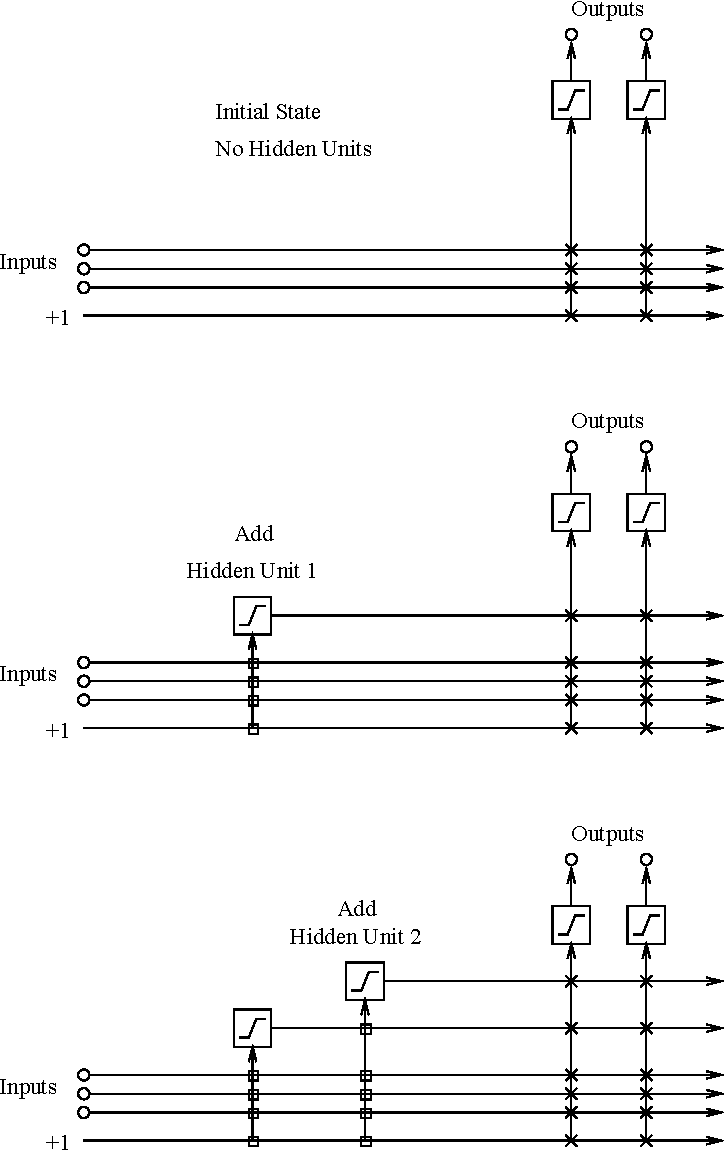
\includegraphics{Figs/PDF/fahlmancascade}
	% 	\caption[Cascade correlation]{\textbf{Cascade Correlation.} Connections marked with a $\square$ are frozen, while $\times$ connections are learned continuously. \copyright \citet{Fahlman1989}}
	% 	\label{fig:cascadecorrelation}
	% 	\mynote{TODO: replace this with our own figure, or remove?}
	% \end{figure}
	
	At the beginning of training only the input and output layers exist,
	% as shown in \cref{fig:cascadecorrelation} %
	and since this is a single-layer network with no hidden units, any of the simpler perceptron training rules can be used. After sufficient training, which is heuristically determined, the network is expanded by a single new hidden unit at a time.
	Each new (candidate) hidden unit that is added to the network is connected to all the network inputs, in addition to all of the outputs of the previous hidden units. The candidate unit is treated as a new hidden layer, and since all other connections are frozen, can be trained as if it was a single-layer --- \ie with the delta rule\index{delta rule}, or other similar single-layer training algorithm, rather than backpropagation\index{backpropagation}. The candidate unit's input weights are adjusted so as to maximize the covariance of the candidate unit's output with the error output of the network:
	% http://www.ra.cs.uni-tuebingen.de/SNNS/UserManual/node167.html#SECTION001081200000000000000
	\begin{equation}
	    C = \sum_o \left|\sum_p (y_{po} - \overline{y_o})(E_{po} - \overline{E_o})\right|,
	\end{equation}
	where $y_{po}$ is the output of the output unit o with input pattern p, $E_{po}$ is the error The trained unit's input weights are then frozen after training, and if an error threshold hasn't been met, a new layer is again added.
	
	Since each new neuron\index{neuron} produces a new layer, cascade correlation\index{cascade correlation} leads to very \glspl{dnn}\index{DNN} with low throughput, since each layer is only one neuron\index{neuron} wide, making them very inefficient computationally. Cascade correlation\index{cascade correlation} networks do not seem to generalize as well as standard neural networks\index{neural network}, likely due to their greedy training strategy, as compared to \glspl{dnn}\index{DNN} trained with backpropagation\index{backpropagation} where no weights are frozen during training.

	\subsubsection{Upstart Algorithm}
	The \emph{upstart algorithm}\index{upstart algorithm|textbf} is a method for building binary classification networks, and is guaranteed to find an architecture with perfect training classification. At a high level it sounds like the tiling algorithm\index{tiling algorithm}\cref{tilingalgo}, but instead of building up layers from the input, in the upstart algorithm\index{upstart algorithm} all the neurons in the network are connected directly to the inputs, and new `child' neurons are added to compensate for the misclassification errors of existing `parent' neurons.
	
	Initially the network consists of one neuron that is trained with the \emph{pocket algorithm}\index{pocket algorithm}~\citep{gallant1986optimal}. This `parent' neuron, now frozen, will misclassify some of the training samples, and to correct these two `child' neurons are added. Since the neurons in the upstart algorithm are binary threshold units, the `parent' neuron will either misclassify samples as negative or positive. The two `child' neurons are then trained (also by the pocket algorithm\index{pocket algorithm}) to provide enough of a negative/positive signal to cause the parent neuron to give correct classifications for one or more of the misclassified samples. The `child' neurons become `parents', and their offspring also learn to correct their mistakes. Empirical results showed that the upstart algorithm produces networks with fewer neurons than the tiling algorithm\index{tiling algorithm}.
	
%	\subsection{Hyper-Networks}
%	More recently \citet{hypernetworks} looked at trying to learn a compact representation of a network, much like weight sharing in an \gls{rnn} allows the concise summary of a potentially infinite depth \gls{rnn}.
	
	\section{Pruning Algorithms}
	Rather than the progressive construction of networks, an alternative approach to learning efficient networks is \emph{pruning}, the removal of unimportant network weights after training.

	Amongst the earliest work\footnote{Rumelhart is noted by \citet{hanson1989comparing} to have worked on a similar, albeit unpublished, method.} on pruning was by \citeauthor{sietsma1988neural}, who investigated the effect of pruning weights in very small perceptron networks. The pruning rules were summarized as ``If the output of a unit does not change for any input pattern that unit is not contributing to the solution. If the outputs of any two units are the same or opposite across all patterns the two units duplicate and one can be removed.''~\citep{sietsma1988neural}. Even in these small networks, the complexity of pruning emerges. The authors propose removing weights close to zero, or weights that similarly do not affect the output of the neuron, and removing complementary but opposite (\ie{}duplicate) weights. %It is claimed that aside from being faster, pruned networks are also less noise-sensitive.
	
	There have been many proposals of methods of pruning network connections since~\citep{hanson1989comparing, lecun1989optimal, mozer1989using, mozer1989skeletonization, gorodkin1993quantitative, setiono1997penalty,castellano1997iterative,han2015learning,han2015deep,han2016dsd,ullrich2017soft,} differing mostly on the method of evaluating the saliency of weights, \ie how important each weight is to maintaining generalization.  Here we will cover only a small selection of the most commonly cited methods.
	
	As demonstrated even in the early approach of \citeauthor{sietsma1988neural}, a naive saliency measure, such as weight magnitude, is overly simplistic in practice since it does not account for the larger distributed representation learned in a neural networks\index{neural network} and can lead to a large reduction in accuracy if used for pruning.

    In a typical pruning algorithm, after having trained the network, a saliency measure for each network weight is calculated. The weights are then sorted by saliency, and the lowest saliency parameters are deleted. After this pruning step, the network must again re-trained from scratch. This iterative re-training means that such pruning methods do not scale well to contemporary neural networks\index{neural network} where training times can be measured in weeks.

	The simplest saliency measure would be to simply measure the effect of removing a weight on the training error of the network. For each weight in the network, the training error can be evaluated, and the difference in error used as the saliency measure for that weight. In practice this straightforward method is infeasible however, since we must evaluate over the training set for each weight of the network. For a network with $n$ weights, and $p$ training samples, calculating the saliencies for the whole network in this manner is $\mathcal{O}(np)$~\citep{hanson1989comparing}.
	
	\subsection{Optimal Brain Damage}
    \citet{lecun1989optimal} proposed \gls{obd} to iteratively remove neurons\index{neuron} after training based on a saliency measure that judges the parameters that have the least effect on training error. The authors point out that simply using the magnitude of the weights themselves is equivalent in the limit to having trained with a form of non-proportional weight decay, instead the authors propose a more theoretically justified saliency measure --- they propose measuring the change in the objective function caused by deleting a parameter. Rather than performing the computationally intensive task of re-evaluating the objective for every possible parameter deletion, the second derivative of the objective with respect to the weights is instead used. The authors approximate the derivative of objective function with respect to the weights using the second-order Taylor series expansion, $f(a) = \sum_{n=0}^\infty \frac{f^{(n)}(a)}{n!} (x - a)^n$, of the error:
    % From optimal brain surgeon paper
    % https://papers.nips.cc/paper/647-second-order-derivatives-for-network-pruning-optimal-brain-surgeon.pdf
    % also look at:
    % http://cslt.riit.tsinghua.edu.cn/mediawiki/images/9/9e/131125-OBD-LC-01.pdf
    % http://web.engr.oregonstate.edu/~tgd/classes/534/slides/part10.pdf
    \begin{align}
       \delta E &= \sum_i \frac{\partial E}{\partial w_i} \delta w_i + \frac{1}{2} \sum_i \frac{\partial^2 E}{\partial w_i^2} \delta w_i^2 + \frac{1}{2} \sum_{i\neq j} \frac{\partial^2 E}{\partial w_i \partial w_j} \delta w_i \delta w_j +\mathcal{O}(\|\delta \mathbf{w}\|^3),
    \end{align}
	%
    where $E$ is the objective function, $w_i$ is the $i$th weight. We can write this more compactly in matrix notation,
    \begin{align}
       \delta E &= \left( \frac{\partial E}{\partial \mathbf{w}} \right)^T \delta \mathbf{w} +\frac{1}{2}\delta \mathbf{w}^T \mathbf{H}\, \delta \mathbf{w} +\mathcal{O}(\|\delta \mathbf{w}\|^3),
    \end{align}
	where $\mathbf{w}$ is the vector of network weights, and %$h_{ij}=\partial^2 E / \partial w_i \partial w_j$
	$\mathbf{H}$ is the Hessian\index{Hessian} matrix of second order derivatives. 

    This approximation is infeasible to calculate in practice, mostly due to the size of the Hessian\index{Hessian} matrix which is square in the number of weights. The authors use several assumptions to approximate this in a more computationally efficient manner. Most importantly they use the ``diagonal approximation'' of the Hessian\index{Hessian}, using only the diagonal terms, $h_{ii}=\partial^2 E / \partial w_i^2$. Further, the ``extremal approximation'' assumes that pruning is only done once the training has converged, and so it can be assumed that the first term is zero. Finally they assume that the function is approximately quadratic, and thus higher order terms (\ie $\mathcal{O}(\|\delta \mathbf{w}\|^3)$) can be ignored. In all, the final approximation of the objective function's change is simply:

    \begin{align}
       \delta E &\approx \frac{1}{2} \sum_i \frac{\partial^2 E}{\partial w_i^2} \delta w_i^2.
    \end{align}
	%
    To calculate the second derivative, chain rule is used, and the second derivatives are back-propagated through the network. This approximation is used directly as the saliency measure for each network weight $w_i$, and after having trained the network, the weights are sorted by saliency, and the lowest saliency parameters are deleted.
	
	\subsection{Gating}
    \citet{hanson1989comparing} proposed using a per-neuron\index{neuron} gating mechanism to measure saliency
    
	\mynote{TODO}
	\citet{ullrich2017soft,}
	%,Xing2009??
	\section{Compression \& Quantization}
	In order to use deep neural networks\index{neural network} on embedded devices, and in many applications, first a more compact representation and perhaps even faster inference is often required. 
	Although mostly a matter of engineering, compression of neural networks\index{neural network} also tells us something about the information theoretic capacity of the models we train, and therefore gives us hints about the internal representation learned in \glspl{dnn}\index{DNN}.

	There have been many papers on the topic~\citep{han2015learning,han2016dsd}, here we will only cover a few of the most cited papers.
	
	\subsection{Learning both Weights and Connections}
	\citet{han2015learning} looked at combining a naive weight magnitude-based pruning method with both quantization and Huffman coding. In all the method can take a trained network
	\mynote{TODO}

	\subsection{Deep-Sparse-Dense Training}
	\citet{han2016dsd}
	\mynote{TODO}
	\subsection{XOR-Net: Binary Convolutional Neural Networks}
	\citet{rastegari2016xnor} proposed two methods, one in which filter parameters were quantized to binary values, from the typical 16-bit floating point representation. Surprisingly even when the method was applied to models trained on \gls{ilsvrc}, such as \gls{alexnet}, the accuracy was little effected.
	\mynote{TODO}
	
\section{Structural Priors}
	This section has shown that the concept we have denoted `structural priors' is not new, and has varied interpretations. Here we will attempt to summarize the concepts covered by this large body of work in a compact nomenclature. While, like with any compact nomenclature, there is a danger of overly simplifying the details, it can also help in seeing the big picture.
	\mynote{TODO: change this section}
    
	In practice when fitting a curve, we have little idea of what order polynomial would best fit the data. Necessarily, we must use a relatively higher order curve to fit the data. Similarly, with a neural network\index{neural network} we rarely have knowledge of the underlying structure of the solution (but when we do, we should use it to parametrize our models appropriately~\citep{jain2016structural}). Instead we must use networks with more parameters than necessary to ensure that there is enough capacity to learn the underlying, but likely sparse solution. The problem with this approach is that over-parametrization of a model generally leads to poor generalization due to overfitting. To prevent this, there are two general types of methods in which we can relate our prior knowledge that the model is over-parametrized to the optimization:
	\begin{description}
	\item[Weak Structural Prior: Regularization]
	Knowing only that our model is over-parametrized is a relatively weak prior, however we can encode this into the fit by using a regularization penalty. This restricts the model to effectively use only a small number of the parameters by adding a penalty, for example on the L2 norm of the model weights. For polynomial regression, this is called \emph{ridge regression}, while for neural networks it is called \emph{weight decay}~\citep{hinton1987learning}. In neural networks early stopping\index{early stopping} during training is another method for doing this.
	
	\item[Strong Structural Prior: Restricted Connectivity]
	With more prior information on the task, \ie when fitting a polynomial, we may ascertain that a certain order polynomial is more appropriate from the convexity of the polynomial, and restrict learning to that order. For example, given samples from a polynomial appear to be convex, we can surmise that the polynomial is likely to be of an even or \engordnumber{2}-order, and restrict our fit to be of that order. 

	In neural networks, as we have seen in \cref{cnns}, a similar effect can be achieved by \emph{removing parameters} that we know are not needed (\ie  in \glspl{cnn}, using filters with local connectivity), or \emph{sharing parameters} we know are redundant (\ie in \glspl{cnn}, using the same filters for all pixels)
    \end{description}
    
	Although neural networks\index{neural network} are usually posed as general learning machines, time and again it has been demonstrated that neural networks\index{neural network} only truly stand out as a learning method when we use strong structural priors, encoding our prior knowledge of the task in the architecture itself. As observed by \citet{denker1987large} this may be considered closer to modifying the problem to be solved itself, rather than changing the learning method. For example, by asking a \gls{cnn} to learn to classify a dataset, we are asking the network to ``classify these images'', whereas by asking a fully-connected network to classify the same dataset, we are asking the network ``classify this data''. The first task is inherently easier.

    Structural priors may be considered one of the greatest contributions to the success of deep learning, but arguably can also be considered the cause of its greatest failure. Structural priors allow deep models to more easily learn specific tasks, \ie image classification or speech recognition. At the same time, by specializing our networks, we are moving further away from the goal of general artificial intelligence\index{general AI}, \ie learning models that can do both tasks.
    
\section{Other Notable Works}
\subsection{Pruning}
\citep{mozer1989using, mozer1989skeletonization, castellano1997iterative,gorodkin1993quantitative,han2016dsd,han2015learning,setiono1997penalty,}

\subsection{Network Size and Generalization}
\citep{denker1987large, giles1987learning, hinton1987learning, lecun1989generalization, ahmad1989scaling,hanson1989comparing,}

\subsection{Structural Priors}
\citep{Fuk80,lecun1989backpropagation,}

\subsection{Compression}
\citep{han2015deep,Kim2016,ullrich2017soft,}

\subsection{TODO}
\citep{mackay1992practical,schwartz1990exhaustive,}

\mynote{Use these references!}
    % \section{Quotes}
    
	% \begin{chapquote}{David Rumelhart, \textit{in personal communication with \citet{hanson1989comparing}, 1987}}
	% ``\ldots the simplest most robust network which accounts for a data set will, on average, lead to the best generalization to the population from which the training set has been drawn''
	% \end{chapquote}
	
	
%	\begin{chapquote}{John Denker \etal, \textit{Large Automatic Learning, Complex Systems, 1987}}
%		``A general tabula rasa network is a fine subject for the abstract, formal studies, but one should not try to use it to solve practical problems. \ldots One should pre-program the network with all available information about the structure of the problem, especially information about the symmetry and topology of the data.''
%	\end{chapquote}
	
	
	% \begin{chapquote}{Mozer \etal, \textit{Using Relevance to Reduce Network Size Automatically, 1989}}
	% ``One thing that connectionist networks have in common with brains is that if you open them up and peer inside, all you can see is a big pile of goo.''
	% \end{chapquote}
	
	
	% \begin{chapquote}{David MacKay, \textit{A Practical Bayesian Framework for Backprop Networks, 1991}}
	% 	``There are many knobs on the black box of `backprop' (learning by backpropagation\index{backpropagation} of
	% 	errors). Generally these knobs are set by rules of thumb, trial and error, and the use of reserved test data to assess generalization ability (or more sophisticated cross-validation).''
	% \end{chapquote}
	
    
	% \begin{chapquote}{Kunihiko Fukushima, \textit{Neocognitron, 
	% 			%A Self-organizing Neural Network Model
	% 			%for a Mechanism of Pattern Recognition
	% 			%Unaffected by Shift in Position , 
	% 			Biol.\ Cybernetics, 1980}}
	% 	`` One of the largest and long-standing difficulties in designing a pattern-recognizing machine has been the problem how to cope with the shift in position and the distortion in shape of the input patterns. The Neocognitron proposed in this paper gives a drastic solution to this difficulty.
	% 	''
	% \end{chapquote}
	
%	\begin{chapquote}{Hubel \& Wiesel ,\textit{Receptive Fields of Single Neurones in the Cat's Striate Cortex, 1959}}
%	``The phenomena of summation and antagonism within receptive fields seem
%to provide a basis for the specificity of stimuli, in shape, size and orientation.
%Units activated by slits and boundaries may converge upon units of higher
%order which require still more complex stimuli for their activation. Most units
%presented in this paper have had receptive fields with clearly separable
%excitatory and inhibitory areas. However, a number of units recorded in the
%striate cortex could not be understood solely in these terms. These units with
%more complex properties are now under study.''
%	\end{chapquote}

	% \begin{chapquote}{Yann LeCun, \textit{Backpropagation Applied to Handwritten Zip Code Recognition, 1989}}
	% 	``Classical work in visual pattern recognition has demonstrated the advantage of extracting local features and combining them to form higher order features. Such knowledge can be easily built into the network by forcing the hidden units to combine only local sources of information. Distinctive features of an object can appear at various location on the input image. Therefore it seems judicious to have a set of feature detectors that can detect a particular instance of a feature anywhere on the input place. Since the precise location of a feature is not relevant to the classification, we can afford to lose some position information in the process. Nevertheless, approximate position information must be preserved, to allow the next levels to detect higher order, more complex features.''
	% \end{chapquote}
	
	
% 	\mynote{Fit this into our talk of learning basis functions/filters!}
% 	\begin{chapquote}{Chris Bishop, \textit{Neural Networks for Pattern Recognition, Page 98, 1996}}
% 	    ``We have already seen that a network with a single-layer of weights has very
% limited capabilities. To improve the performance of the perceptron, Rosenblatt
% used a layer of fixed processing elements to transform the raw input data, as
% shown in Figure 3.10. These processing elements can be regarded as the basis
% functions of a generalized linear discriminant.''
% 	\end{chapquote}
\end{document}
